\documentclass[11pt,a4paper,twoside]{book}
\usepackage[T1]{fontenc}
\usepackage[utf8]{inputenc}
\usepackage{mathpazo}
\usepackage[scaled=0.90]{helvet}
\usepackage{courier}
\usepackage[a4paper,inner=3.0cm,outer=2.4cm,top=2.6cm,bottom=2.8cm]{geometry}
\usepackage{xcolor}
\usepackage{mathtools}
\usepackage{colortbl}
\usepackage{tikz}
\usetikzlibrary{calc,positioning,arrows.meta,decorations.pathmorphing}
\usepackage{booktabs}
\usepackage{array}
\usepackage{longtable}
\usepackage{enumitem}
\usepackage[german=quotes]{csquotes}
\usepackage{fancyhdr}
\usepackage{titlesec}
\usepackage{amsmath,amssymb}
\usepackage{tcolorbox}
\tcbuselibrary{skins,breakable}
\usepackage[hidelinks]{hyperref}

\definecolor{tief}{HTML}{1F3A5F}
\definecolor{mittel}{HTML}{2E5F8A}
\definecolor{akzent}{HTML}{A34A28}
\definecolor{sand}{HTML}{F4F1EA}
\definecolor{grau}{HTML}{5A5A5A}
\definecolor{gruen}{HTML}{2F6B4F}
\definecolor{purpur}{HTML}{5B3A72}

\newcolumntype{P}[1]{>{\raggedright\arraybackslash}p{#1}}

\newcommand{\kursiv}[1]{{\itshape\color{grau}#1}}
\newcommand{\code}[1]{{\ttfamily\small #1}}
\newcommand{\Person}[1]{\textbf{#1}}
\newcommand{\Begriff}[1]{\textbf{#1}}
\newcommand{\zit}[1]{\textsuperscript{[#1]}}
\newcommand{\Oh}{\mathcal{O}}
\newcommand{\boxtitel}[1]{{\bfseries\color{tief}#1}\par\vspace{6pt}}
\newcommand{\boxtitelr}[1]{{\bfseries\color{akzent}#1}\par\vspace{6pt}}
\newcommand{\boxtitelg}[1]{{\bfseries\color{gruen}#1}\par\vspace{6pt}}
\newcommand{\boxtitelp}[1]{{\bfseries\color{purpur}#1}\par\vspace{6pt}}
\newcommand{\boxtitelm}[1]{{\bfseries\color{mittel}#1}\par\vspace{6pt}}
\newcommand{\loesung}{\par\vspace{8pt}{\bfseries\color{mittel}Lösung}\par\vspace{4pt}}
\newcommand{\schritt}[1]{\par\vspace{5pt}{\bfseries\color{grau}#1}\par\vspace{2pt}}

% Graphentheoretische Notation
\newcommand{\Gr}{G}
\newcommand{\Kn}[1]{K_{#1}}
\newcommand{\Kmn}[2]{K_{#1,#2}}
\newcommand{\Grad}{\deg}
\newcommand{\Nb}{N}
\newcommand{\chrom}{\chi}
\newcommand{\Ecken}{V}
\newcommand{\Kanten}{E}

\newtcolorbox{grundbox}[1][tief]{
  breakable, enhanced, colback=sand, colframe=sand,
  boxrule=0pt, leftrule=3pt, borderline west={3pt}{0pt}{#1},
  left=12pt, right=10pt, top=10pt, bottom=10pt,
  sharp corners, before skip=12pt, after skip=12pt}

\newenvironment{merksatz}{\begin{grundbox}[tief]}{\end{grundbox}}
\newenvironment{warnung}{\begin{grundbox}[akzent]}{\end{grundbox}}
\newenvironment{definition}{\begin{grundbox}[mittel]}{\end{grundbox}}
\newenvironment{geschichte}{\begin{grundbox}[gruen]}{\end{grundbox}}
\newenvironment{forschung}{\begin{grundbox}[purpur]}{\end{grundbox}}
\newenvironment{aufgabe}{\begin{grundbox}[grau]}{\end{grundbox}}
\newenvironment{technik}{\begin{grundbox}[mittel]}{\end{grundbox}}

\titleformat{\chapter}[display]
  {\normalfont\huge\bfseries\color{tief}}{\Large\color{grau}Kapitel \thechapter}{8pt}{\Huge}
\titleformat{\part}[display]
  {\normalfont\huge\bfseries\color{tief}\filcenter}{\Large\color{grau}Teil \thepart}{10pt}{\Huge}
\titlespacing*{\chapter}{0pt}{10pt}{28pt}

\pagestyle{fancy}
\fancyhf{}
\fancyhead[LE,LO]{\small\itshape\color{grau}\leftmark}
\fancyfoot[LE,LO]{\small\color{grau}\thepage}
\renewcommand{\headrulewidth}{0.4pt}
\renewcommand{\footrulewidth}{0pt}
\renewcommand{\chaptermark}[1]{\markboth{#1}{}}
\setlength{\parindent}{0pt}
\setlength{\parskip}{6pt}
\renewcommand{\arraystretch}{1.3}

\renewcommand{\contentsname}{Inhaltsverzeichnis}
\renewcommand{\chaptername}{Kapitel}
\renewcommand{\partname}{Teil}
\renewcommand{\appendixname}{Anhang}
\renewcommand{\tablename}{Tabelle}
\renewcommand{\figurename}{Abbildung}

\hyphenation{Ver-all-ge-mei-ne-rung ver-all-ge-mei-nern Über-an-pas-sung Kreuz-va-li-die-rung
Trai-nings-da-ten Test-da-ten Hy-po-the-sen-klas-se Ver-lust-funk-ti-on Klas-si-fi-ka-tor
Klas-si-fi-ka-ti-on Re-gu-la-ri-sie-rung Ent-schei-dungs-baum Ent-schei-dungs-bäu-me
Stütz-vek-tor Stütz-vek-tor-ma-schi-ne Kern-me-tho-de Haupt-kom-po-nen-ten
Rück-pro-pa-ga-ti-on Gra-di-en-ten-ab-stieg Neu-ro-nal neu-ro-na-le Clus-ter-bil-dung
Di-men-si-ons-re-duk-ti-on Sep-sis-Früh-war-nung Lak-tat Über-pa-ra-me-tri-sie-rung
Neu-stadt Kli-ni-kum Emp-find-lich-keit Trenn-schär-fe}

\tikzset{
  knoten/.style={circle, fill=tief, inner sep=0pt, minimum size=5.5pt},
  knotenb/.style={circle, draw=tief, fill=white, line width=0.9pt, inner sep=1pt, minimum size=15pt, font=\scriptsize},
  knotenr/.style={circle, draw=akzent, fill=akzent!12, line width=0.9pt, inner sep=1pt, minimum size=15pt, font=\scriptsize},
  knoteng/.style={circle, draw=gruen, fill=gruen!12, line width=0.9pt, inner sep=1pt, minimum size=15pt, font=\scriptsize},
  kante/.style={draw=grau, line width=0.9pt},
  kanted/.style={draw=akzent, line width=1.5pt},
}

\newcommand{\MW}{\overline{x}}
\newcommand{\dd}{\mathrm{d}}
\newcommand{\R}{\mathbb{R}}
\newcommand{\Z}{\mathbb{Z}}
\newcommand{\Ent}{H}
\newcommand{\vek}[1]{\boldsymbol{#1}}
\newcommand{\lb}{\operatorname{ld}}



\newcommand{\Risk}{\mathcal{R}}
\newcommand{\Hyp}{\mathcal{H}}
\newcommand{\E}{\mathbb{E}}

\begin{document}
\frontmatter
\begin{titlepage}
\centering
\vspace*{1.6cm}
{\footnotesize\scshape\color{grau} Mathematik von Grund auf --- Band 22}\\[1.9cm]
{\Huge\bfseries\color{tief} Was sich}\\[6pt]
{\Huge\bfseries\color{tief} verallgemeinern lässt}\\[16pt]
{\Large\color{akzent} Maschinelles Lernen}\\[1.3cm]

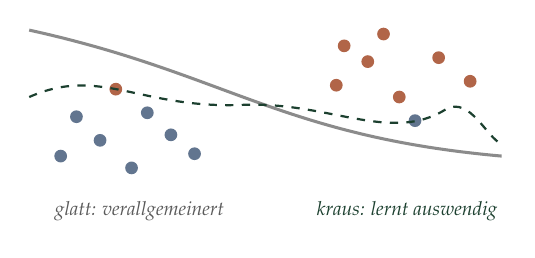
\begin{tikzpicture}[scale=1.0]
\foreach \x/\y in {-2.6/0.35,-2.1/0.55,-1.7/0.2,-1.2/0.62,-0.9/0.38,-2.4/0.85,-1.5/0.9}
  \fill[tief!70] (\x,\y) circle (2.3pt);
\foreach \x/\y in {0.9/1.25,1.3/1.55,1.7/1.1,2.2/1.6,1.5/1.9,2.6/1.3,1.0/1.75}
  \fill[akzent!85] (\x,\y) circle (2.3pt);
\fill[akzent!85] (-1.9,1.2) circle (2.3pt);
\fill[tief!70] (1.9,0.8) circle (2.3pt);
\draw[grau!70, line width=1.1pt] (-3.0,1.95) .. controls (-0.5,1.4) and (0.2,0.6) .. (3.0,0.35);
\draw[gruen!60!black, line width=0.8pt, dashed] (-3.0,1.1) .. controls (-2.1,1.5) and (-1.6,0.95) .. (-0.3,1.0)
   .. controls (0.8,1.05) and (1.6,0.5) .. (2.3,0.95) .. controls (2.6,1.1) and (2.8,0.6) .. (3.0,0.5);
\node[font=\scriptsize\itshape, color=grau] at (-1.6,-0.35) {glatt: verallgemeinert};
\node[font=\scriptsize\itshape, color=gruen!60!black] at (1.8,-0.35) {kraus: lernt auswendig};
\end{tikzpicture}

\vspace{1.3cm}
{\large\color{grau} Von der Bayes-Regel bis zum tiefen Netz}\\[6pt]
{\color{grau} Jeder Schritt erklärt. Mit vollständig durchgerechneten Übungsaufgaben.}\\[1.9cm]
{\small\color{grau} Stand der Forschung: August 2026}
\end{titlepage}
\thispagestyle{empty}
\vspace*{\fill}
\begin{flushleft}
{\small\color{grau}
\textbf{\color{tief}Mathematik von Grund auf} --- Band 22\\[2pt]
\textit{Was sich verallgemeinern lässt} $\cdot$ Maschinelles Lernen\\[14pt]

Herausgeber und Urheber: Jürgen Maier\\[2pt]
Entstanden 2026 in Zusammenarbeit mit Claude (Anthropic); Konzeption, Vorgaben, Prüfung und Herausgeberschaft: Jürgen Maier.\\[14pt]

\textbf{Lizenz}\\[2pt]
Dieses Werk ist lizenziert unter einer Creative-Commons-Lizenz \textbf{Namensnennung -- Weitergabe unter gleichen Bedingungen 4.0 International (CC BY-SA 4.0)}. Sie dürfen das Werk vervielfältigen, verbreiten, bearbeiten und auch kommerziell nutzen, sofern Sie den Urheber nennen und Bearbeitungen unter derselben Lizenz weitergeben.\\[2pt]
Lizenztext: \texttt{https://creativecommons.org/licenses/by-sa/4.0/legalcode.de}\\[14pt]

\textbf{Quellen und Fassungen}\\[2pt]
Quelltexte, Simulationen, Fehlermeldungen und aktuelle Fassungen aller Bände:\\
\texttt{https://github.com/juergenmaier2026/mathematik-von-grund-auf}\\[2pt]
Dauerhaft archiviert bei Zenodo: \texttt{https://doi.org/10.5281/zenodo.23698547}\\[14pt]

\textbf{Zitiervorschlag}\\[2pt]
Maier, J. (2026). \textit{Mathematik von Grund auf, Band 22: Was sich verallgemeinern lässt}. Fassung 1.0.1. \texttt{https://doi.org/10.5281/zenodo.23698547}\\[14pt]

Satz: \LaTeX{} mit Palatino. Fassung 1.0.1, Oktober 2026. 204 Seiten.
}
\end{flushleft}
\vspace*{1.5cm}

\tableofcontents
\mainmatter

\chapter*{Vorwort}
\addcontentsline{toc}{chapter}{Vorwort}

\begin{merksatz}
\boxtitel{Eine alte Frage mit neuem Werkzeug}
Aus hundert Beobachtungen soll eine Regel gewonnen werden, die auch für die hunderterste stimmt.

\begin{center}
\begin{minipage}{0.9\textwidth}
\textbf{Das ist die Frage dieses Bandes. Sie ist so alt wie die Wissenschaft --- und sie hat keine allgemeine Antwort.}
\end{minipage}
\end{center}

\begin{center}
\begin{minipage}{0.88\textwidth}
\kursiv{David Hume bemerkte 1739, dass kein Schluss von Beobachtetem auf Unbeobachtetes logisch zwingend ist. \textbf{Das maschinelle Lernen hat dieses Problem nicht gelöst, sondern präzisiert}: Es gibt an, unter welchen Annahmen der Schluss gelingt, wie viele Beobachtungen er braucht und wie groß der Fehler höchstens ist. Das ist weniger, als der Name verspricht, und mehr, als Hume für möglich hielt.}
\end{minipage}
\end{center}
\end{merksatz}

\begin{merksatz}
\boxtitel{Wo der Band steht}
\begin{center}
{\small
\renewcommand{\arraystretch}{1.5}
\begin{tabular}{@{}P{2.2cm}P{6.4cm}@{}}
\toprule
\textbf{Band 17} & Statistik fragt: Was sagen diese Daten über die Welt? Man schätzt Parameter eines Modells, das man vorher festlegt.\\
\textbf{Band 19} & Optimierung fragt: Welche Wahl ist die beste? Die Zielfunktion ist gegeben.\\
\textbf{Band 20} & Informationstheorie fragt: Wie kurz lässt sich etwas beschreiben?\\
\textbf{Hier} & Lernen fragt: Welche Regel wird auf \kursiv{neuen} Daten am besten abschneiden --- ohne dass man das Modell vorher kennt?\\
\bottomrule
\end{tabular}}
\end{center}

\begin{center}
\begin{minipage}{0.9\textwidth}
\textbf{Dieser Band ist der erste der Reihe, der vier Vorgängerbände zugleich benutzt.}
\end{minipage}
\end{center}

\begin{center}
\begin{minipage}{0.88\textwidth}
\kursiv{Schätzen kommt aus Band 17, das Minimieren aus Band 19, die kürzeste Beschreibung aus Band 20, die Minimax-Formulierung robuster Verfahren aus Band 21. \textbf{Maschinelles Lernen ist kein neues Gebiet, sondern ein Treffpunkt} --- und die meisten seiner Sätze sind Sätze aus diesen Bänden, auf eine neue Frage angewandt.}
\end{minipage}
\end{center}
\end{merksatz}

\begin{merksatz}
\boxtitel{Drei Ergebnisse, die man nicht erwartet}
\begin{center}
{\small
\renewcommand{\arraystretch}{1.55}
\begin{tabular}{@{}P{1.0cm}P{7.4cm}@{}}
\toprule
$1$ & Es gibt kein Lernverfahren, das auf allen Aufgaben besser ist als ein anderes. Wer ohne Annahme lernen will, lernt nichts. \kursiv{(Kapitel 1)}\\
$2$ & Wie viele Beispiele man braucht, hängt nicht von der Zahl der möglichen Regeln ab, sondern von einer einzigen Zahl --- der VC-Dimension. Unendlich viele Regeln können mit endlich vielen Beispielen lernbar sein. \kursiv{(Kapitel 7)}\\
$3$ & Tiefe Netze mit mehr Parametern als Beispielen verallgemeinern gut --- entgegen allem, was die Theorie der ersten beiden Teile vorhersagt. Warum, ist nicht verstanden. \kursiv{(Kapitel 14)}\\
\bottomrule
\end{tabular}}
\end{center}

\begin{center}
\begin{minipage}{0.88\textwidth}
\kursiv{Das dritte Ergebnis ist die Lage, in der sich das Fach heute befindet. \textbf{Die erfolgreichsten Verfahren sind die am schlechtesten verstandenen}, und die Theorie, die dieser Band entwickelt, erklärt die ältere Hälfte des Fachs vollständig und die neuere kaum. Das ist keine Schwäche der Darstellung, sondern der Stand.}
\end{minipage}
\end{center}
\end{merksatz}

\begin{merksatz}
\boxtitel{Die sechs Teile}
\begin{center}
{\small
\renewcommand{\arraystretch}{1.5}
\begin{tabular}{@{}P{1.4cm}P{3.0cm}P{3.6cm}@{}}
\toprule
\textbf{Teil} & \textbf{Thema} & \textbf{Kapitel}\\
\midrule
I & Das Problem & $1$--$3$\\
II & Lineare Verfahren & $4$--$6$\\
III & Die Theorie & $7$--$8$\\
IV & Nichtlineare Verfahren & $9$--$11$\\
V & Ohne Etiketten, in der Tiefe & $12$--$14$\\
VI & Stand & $15$\\
\bottomrule
\end{tabular}}
\end{center}

\schritt{Der Leitfall}
Das Klinikum Neustadt will eine Sepsis früh erkennen --- aus Laborwerten und Vitalparametern, bevor die Diagnose klinisch offensichtlich wird.

\begin{center}
\begin{minipage}{0.88\textwidth}
\kursiv{Der Leitfall ist nicht erfunden. \textbf{Ein weit verbreitetes kommerzielles Sepsis-Warnsystem wurde 2021 an einer unabhängigen Klinik nachgeprüft} --- und erkannte zwei Drittel der Fälle nicht, bei einer Alarmflut, die das Personal zu ignorieren lernte. Der Band nimmt diese Geschichte als Maßstab: Jedes Verfahren wird daran gemessen, ob es dasselbe Schicksal erleiden würde.}
\end{minipage}
\end{center}
\end{merksatz}

\begin{warnung}
\boxtitelr{Drei Warnungen}
\begin{center}
{\small
\renewcommand{\arraystretch}{1.55}
\begin{tabular}{@{}P{2.2cm}P{6.4cm}@{}}
\toprule
\textbf{Erste} & Ein Verfahren lernt, was in den Daten steht --- nicht, was man gemeint hat. Wer die falschen Daten liefert, bekommt eine gut begründete falsche Antwort.\\
\textbf{Zweite} & Gute Ergebnisse auf den Trainingsdaten sagen nichts. Gute Ergebnisse auf Testdaten sagen etwas --- über Daten, die so aussehen wie die Testdaten.\\
\textbf{Dritte} & Vorhersage ist nicht Erklärung. Ein Verfahren, das richtig vorhersagt, muss nicht verstanden haben, warum.\\
\bottomrule
\end{tabular}}
\end{center}

\begin{center}
\begin{minipage}{0.88\textwidth}
\kursiv{Die zweite Warnung ist die wichtigste und die am häufigsten verletzte. \textbf{Das Sepsis-Warnsystem von 2021 war auf den Daten seiner Entwickler gut} --- nur sahen die Daten der prüfenden Klinik anders aus. Wer über ein Lernverfahren spricht, muss sagen, auf welchen Daten es geprüft wurde, und wie ähnlich diese denen sind, auf die es angewandt werden soll.}
\end{minipage}
\end{center}
\end{warnung}

\begin{merksatz}
\boxtitel{Was dieser Band voraussetzt}
\begin{center}
{\small
\renewcommand{\arraystretch}{1.48}
\begin{tabular}{@{}P{3.0cm}P{1.6cm}P{3.0cm}@{}}
\toprule
\textbf{Werkzeug} & \textbf{Band} & \textbf{gebraucht in}\\
\midrule
Wahrscheinlichkeit & $4$ & durchgehend\\
Matrizen, Eigenwerte & $2$ & Kapitel 4, 6, 13\\
Ableitungen, Gradient & $3$ & Kapitel 4, 11\\
Schätzen, Testen & $17$ & Kapitel 2, 3, 4\\
Konvexität, Dualität & $19$ & Kapitel 5, 6\\
Entropie & $20$ & Kapitel 9, 12\\
\bottomrule
\end{tabular}}
\end{center}

\begin{center}
\begin{minipage}{0.88\textwidth}
\kursiv{\textbf{Wer nur Band 0 und die Grundzüge von Band 4 kennt, kommt durch Teil~I}, und die weiteren Voraussetzungen werden jeweils dort genannt, wo sie gebraucht werden. Wo ein Satz aus einem Vorgängerband benutzt wird, steht die Fundstelle dabei.}
\end{minipage}
\end{center}
\end{merksatz}

\part{Das Problem}

\chapter{Was Lernen heißt}

\section{Der Leitfall}

\begin{merksatz}
\boxtitel{Sepsis-Frühwarnung aus einem einzigen Wert}
Auf der Intensivstation des Klinikums wird bei jedem Patienten das Laktat bestimmt. Etwa jeder zehnte entwickelt in den folgenden Stunden eine Sepsis.

\begin{center}
{\small
\renewcommand{\arraystretch}{1.5}
\begin{tabular}{@{}P{2.4cm}P{2.2cm}P{3.2cm}@{}}
\toprule
\textbf{Gruppe} & \textbf{Anteil} & \textbf{Laktat in mmol/l}\\
\midrule
ohne Sepsis & $90\,\%$ & um $1{,}2$, Streuung $0{,}5$\\
mit Sepsis & $10\,\%$ & um $3{,}0$, Streuung $1{,}0$\\
\bottomrule
\end{tabular}}
\end{center}

\textbf{Die Frage:} Ab welchem Laktatwert soll gewarnt werden?

\begin{center}
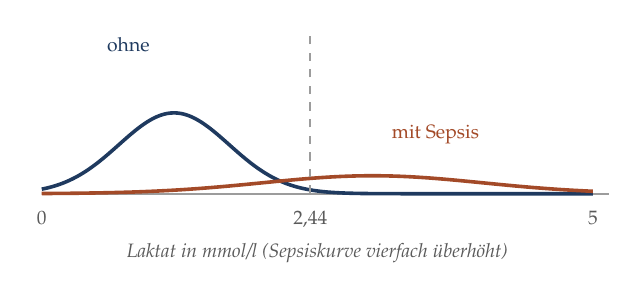
\begin{tikzpicture}[scale=1.0]
\draw[grau!60, line width=0.7pt] (0,0) -- (7.2,0);
\draw[tief, line width=1.3pt, smooth, samples=80, domain=0:7]
  plot ({\x}, {2.6*0.9*exp(-((\x/1.4-1.2)^2)/(2*0.25))/(0.5*2.5066)*0.55});
\draw[akzent, line width=1.3pt, smooth, samples=80, domain=0:7]
  plot ({\x}, {2.6*0.1*exp(-((\x/1.4-3.0)^2)/(2*1.0))/(1.0*2.5066)*0.55*4});
\draw[grau!60, line width=0.8pt, dashed] (3.41,0) -- (3.41,2.0);
\node[font=\scriptsize, color=tief] at (1.1,1.9) {ohne};
\node[font=\scriptsize, color=akzent] at (5.0,0.75) {mit Sepsis};
\node[font=\scriptsize, color=grau, anchor=north] at (3.41,-0.1) {$2{,}44$};
\node[font=\scriptsize, color=grau, anchor=north] at (0,-0.1) {$0$};
\node[font=\scriptsize, color=grau, anchor=north] at (7.0,-0.1) {$5$};
\node[font=\scriptsize\itshape, color=grau] at (3.5,-0.75) {Laktat in mmol/l (Sepsiskurve vierfach überhöht)};
\end{tikzpicture}
\end{center}

\begin{center}
\begin{minipage}{0.88\textwidth}
\kursiv{Die beiden Verteilungen überlappen. \textbf{Es gibt keine Schwelle, die alle richtig einordnet} --- jede Wahl erkauft weniger Fehlalarme mit mehr übersehenen Fällen oder umgekehrt. Die Frage ist also nicht, wie man Fehler vermeidet, sondern welche man in Kauf nimmt.}
\end{minipage}
\end{center}
\end{merksatz}

\section{Die Bestandteile}

\begin{definition}
\boxtitelm{Definition 1.1 --- die Lernaufgabe}
\begin{center}
{\small
\renewcommand{\arraystretch}{1.55}
\begin{tabular}{@{}P{2.6cm}P{6.0cm}@{}}
\toprule
\textbf{Merkmale} & $x \in \mathcal X$ --- was man beobachtet, hier der Laktatwert.\\
\textbf{Zielgröße} & $y \in \mathcal Y$ --- was man vorhersagen will, hier Sepsis ja oder nein.\\
\textbf{Verteilung} & $P$ auf $\mathcal X \times \mathcal Y$ --- \textcolor{akzent}{unbekannt}.\\
\textbf{Regel} & $h: \mathcal X \to \mathcal Y$ --- auch \Begriff{Hypothese} oder \Begriff{Klassifikator}.\\
\textbf{Verlust} & $L(h(x),y)$ --- was ein Fehler kostet.\\
\textbf{Daten} & $(x_1,y_1),\ldots,(x_n,y_n)$ unabhängig aus $P$ gezogen.\\
\bottomrule
\end{tabular}}
\end{center}
\end{definition}

\begin{merksatz}
\boxtitel{Was an dieser Definition wichtig ist}
\begin{center}
\begin{minipage}{0.9\textwidth}
\textbf{Die Verteilung $P$ ist unbekannt.} Man sieht nur die $n$ Beispiele.
\end{minipage}
\end{center}

\begin{center}
\begin{minipage}{0.88\textwidth}
\kursiv{Das unterscheidet das Lernen von der Statistik aus Band 17. Dort nahm man an, $P$ gehöre zu einer bestimmten Familie --- etwa den Normalverteilungen --- und schätzte deren Parameter. \textbf{Hier nimmt man über $P$ möglichst wenig an}, und gerade deshalb ist die Frage schwer. Im Leitfall kennen wir $P$ nur, weil wir es vorgegeben haben; das Klinikum kennt es nicht.}
\end{minipage}
\end{center}

\schritt{Die letzte Zeile ist die stärkste Annahme}
\begin{center}
\begin{minipage}{0.88\textwidth}
\kursiv{\enquote{Unabhängig aus $P$ gezogen} heißt: Die Daten, aus denen man lernt, und die, auf die man das Gelernte anwendet, stammen aus \kursiv{derselben} Verteilung. \textbf{Das ist genau die Annahme, die beim Sepsis-System von 2021 verletzt war} --- und sie steht in fast jedem Satz dieses Bandes als stillschweigende Voraussetzung.}
\end{minipage}
\end{center}
\end{merksatz}

\begin{definition}
\boxtitelm{Definition 1.2 --- das Risiko}
Das \Begriff{Risiko} einer Regel ist ihr erwarteter Verlust:
\[ \Risk(h) = \E\bigl[L(h(X),Y)\bigr] . \]
Beim \Begriff{Null-Eins-Verlust} --- ein Fehler kostet eins, ein Treffer null --- ist das
\[ \Risk(h) = \Pr\bigl[h(X) \ne Y\bigr] , \]
die Wahrscheinlichkeit einer Fehleinordnung.
\end{definition}

\begin{merksatz}
\boxtitel{Das Ziel}
\begin{center}
\begin{minipage}{0.9\textwidth}
\textbf{Gesucht ist eine Regel mit kleinem Risiko --- auf Daten, die man noch nicht gesehen hat.}
\end{minipage}
\end{center}

\begin{center}
\begin{minipage}{0.88\textwidth}
\kursiv{Das ist der Kern des Titels. \textbf{Eine Regel, die die gesehenen Daten gut erklärt, ist leicht zu finden} --- man lernt sie einfach auswendig. Eine Regel, die auch auf ungesehenen Daten stimmt, ist das eigentliche Ziel, und die Differenz zwischen beiden ist der Gegenstand der Kapitel~2, 3, 7 und 8.}
\end{minipage}
\end{center}
\end{merksatz}

\section{Die bestmögliche Regel}

\begin{merksatz}
\boxtitel{Wenn man $P$ kennte}
Sei $\eta(x) = \Pr[Y=1 \mid X=x]$ die Wahrscheinlichkeit einer Sepsis beim Laktatwert $x$.

\begin{definition}
\boxtitelm{Definition 1.3 --- Bayes-Regel}
\[ h^{*}(x) = \begin{cases} 1 & \text{falls } \eta(x) \ge \tfrac12\\ 0 & \text{sonst} \end{cases} \]
\end{definition}

\schritt{Satz 1.4 --- sie ist die beste}
Für jede Regel $h$ gilt beim Null-Eins-Verlust
\[ \Risk(h^{*}) \ \le\ \Risk(h) . \]

\schritt{Beweis}
Man betrachtet einen festen Wert $x$. Die Wahrscheinlichkeit eines Fehlers bei gegebenem $x$ ist
\[ \Pr\bigl[h(x) \ne Y \mid X=x\bigr] = \begin{cases} \eta(x) & \text{falls } h(x)=0 \quad\text{(Sepsis übersehen)}\\ 1-\eta(x) & \text{falls } h(x)=1 \quad\text{(Fehlalarm)} \end{cases} \]

\kursiv{Das Kleinere der beiden ist} $\min\{\eta(x),\,1-\eta(x)\}$ --- und genau dieses wählt $h^{*}$: Ist $\eta(x) \ge \tfrac12$, so ist $1-\eta(x)$ das Kleinere, und $h^{*}$ sagt $1$.

\kursiv{Also gilt für jedes $x$:}
\[ \Pr\bigl[h^{*}(x) \ne Y \mid X=x\bigr] \ \le\ \Pr\bigl[h(x) \ne Y \mid X=x\bigr] \]

\kursiv{Mittelung über $x$} erhält die Ungleichung, denn ein Mittelwert kleinerer Zahlen ist kleiner. $\blacksquare$

\begin{center}
\begin{minipage}{0.9\textwidth}
\textbf{Man entscheidet sich an jeder Stelle für das Wahrscheinlichere --- und das ist global optimal.}
\end{minipage}
\end{center}
\end{merksatz}

\begin{merksatz}
\boxtitel{Der Leitfall gerechnet}
\schritt{Die Wahrscheinlichkeit einer Sepsis nach dem Messwert}
Nach dem Satz von Bayes (Band 4):
\[ \eta(x) = \frac{0{,}1\cdot f_1(x)}{0{,}1\cdot f_1(x) + 0{,}9\cdot f_0(x)} \]
mit den Dichten $f_0$ und $f_1$ der beiden Gruppen.

\begin{center}
{\small
\renewcommand{\arraystretch}{1.48}
\begin{tabular}{@{}P{2.2cm}P{2.2cm}P{3.2cm}@{}}
\toprule
\textbf{Laktat} & $\eta(x)$ & \\
\midrule
$1{,}0$ & $0{,}008$ & \\
$1{,}5$ & $0{,}021$ & \\
$2{,}0$ & $0{,}108$ & \\
$2{,}5$ & $0{,}590$ & \textcolor{akzent}{über der Hälfte}\\
$3{,}0$ & $0{,}973$ & \\
\bottomrule
\end{tabular}}
\end{center}

\schritt{Die Schwelle}
Die Bayes-Regel warnt, wo $\eta(x) = \tfrac12$ überschritten wird:
\[ x^{*} = 2{,}44 \ \text{mmol/l} \]

\schritt{Das Bayes-Risiko}
\[ \Risk^{*} = \Risk(h^{*}) = 3{,}47\,\% \]

\begin{center}
{\small
\renewcommand{\arraystretch}{1.5}
\begin{tabular}{@{}P{2.4cm}P{1.8cm}P{2.0cm}P{2.0cm}@{}}
\toprule
\textbf{Schwelle} & \textbf{Fehler} & \textbf{Empf.} & \textbf{Spezif.}\\
\midrule
$1{,}50$ & $25{,}4\,\%$ & $93{,}3\,\%$ & $72{,}6\,\%$\\
$2{,}00$ & $6{,}5\,\%$ & $84{,}1\,\%$ & $94{,}5\,\%$\\
$\mathbf{2{,}44}$ & $\mathbf{3{,}5\,\%}$ & $71{,}4\,\%$ & $99{,}3\,\%$\\
$3{,}00$ & $5{,}0\,\%$ & $50{,}0\,\%$ & $100\,\%$\\
\midrule
nie warnen & $10{,}0\,\%$ & $0\,\%$ & $100\,\%$\\
\bottomrule
\end{tabular}}
\end{center}

\begin{center}
\begin{minipage}{0.9\textwidth}
\textbf{Die beste mögliche Regel übersieht fast drei von zehn Sepsisfällen.}
\end{minipage}
\end{center}

\begin{center}
\begin{minipage}{0.88\textwidth}
\kursiv{Und sie ist nur um den Faktor drei besser als die Regel \enquote{nie warnen}, die ohne jede Messung auskommt. \textbf{Das Bayes-Risiko ist eine untere Schranke für jedes Verfahren} --- kein noch so kluges Lernverfahren kommt darunter, solange es nur das Laktat kennt. Wer bessere Vorhersagen will, braucht mehr Merkmale, nicht ein besseres Verfahren.}
\end{minipage}
\end{center}
\end{merksatz}

\section{Wenn Fehler verschieden kosten}

\begin{merksatz}
\boxtitel{Eine übersehene Sepsis ist schlimmer als ein Fehlalarm}
Kostet ein übersehener Fall $c_{\text{FN}}$ und ein Fehlalarm $c_{\text{FP}}$, so lautet die Bayes-Regel
\[ h^{*}(x) = 1 \quad\Longleftrightarrow\quad \eta(x) \ \ge\ \frac{c_{\text{FP}}}{c_{\text{FP}}+c_{\text{FN}}} . \]

\schritt{Warum}
Dieselbe Rechnung wie in Satz 1.4, nur mit Gewichten: Warnen kostet im Mittel $c_{\text{FP}}(1-\eta)$, nicht warnen $c_{\text{FN}}\,\eta$. Man warnt, wenn das Erste kleiner ist:
\[ c_{\text{FP}}(1-\eta) \le c_{\text{FN}}\,\eta \quad\Longleftrightarrow\quad \eta \ge \frac{c_{\text{FP}}}{c_{\text{FP}}+c_{\text{FN}}} \]

\schritt{Im Leitfall mit $c_{\text{FN}} : c_{\text{FP}} = 10 : 1$}
\[ \eta(x) \ \ge\ \frac{1}{11} = 0{,}091 \quad\Longrightarrow\quad x^{*} = 1{,}95 \ \text{mmol/l} \]

\begin{center}
{\small
\renewcommand{\arraystretch}{1.5}
\begin{tabular}{@{}P{2.6cm}P{1.8cm}P{1.8cm}P{2.0cm}@{}}
\toprule
& \textbf{Schwelle} & \textbf{Fehler} & \textbf{Kosten}\\
\midrule
kleinster Fehler & $2{,}44$ & $3{,}5\,\%$ & $0{,}292$\\
kleinste Kosten & $1{,}95$ & $7{,}4\,\%$ & $\mathbf{0{,}207}$\\
\bottomrule
\end{tabular}}
\end{center}

\begin{center}
\begin{minipage}{0.9\textwidth}
\textbf{Die Regel mit den geringsten Kosten macht doppelt so viele Fehler wie die mit den wenigsten Fehlern --- und ist dennoch die bessere.}
\end{minipage}
\end{center}

\begin{center}
\begin{minipage}{0.88\textwidth}
\kursiv{Die Empfindlichkeit steigt dabei von $71$ auf $85$ Prozent. \textbf{Die Wahl der Verlustfunktion ist keine technische Einzelheit, sondern eine medizinische Entscheidung} --- und sie wird in der Entwicklung solcher Systeme häufig nicht getroffen, sondern stillschweigend durch den Null-Eins-Verlust ersetzt. Das ist die erste Warnung des Vorworts in ihrer einfachsten Gestalt.}
\end{minipage}
\end{center}
\end{merksatz}

\section{Kein Lernen ohne Annahme}

\begin{merksatz}
\boxtitel{Satz 1.5 --- kein Verfahren ist überall besser}
Mittelt man über \kursiv{alle} möglichen Zusammenhänge zwischen $x$ und $y$, so haben alle Lernverfahren auf ungesehenen Daten dasselbe mittlere Risiko.

\schritt{Der Gedanke}
Sei $\mathcal X$ endlich und seien die Trainingsdaten gegeben. Auf einem Punkt $x$, der in den Daten nicht vorkommt, kann die Zielgröße jeden Wert haben.

\begin{center}
\begin{minipage}{0.9\textwidth}
\textbf{Ohne Annahme ist jede Vorhersage für $x$ genauso gut wie jede andere} --- im Mittel über alle denkbaren Welten liegt sie in der Hälfte der Fälle richtig.
\end{minipage}
\end{center}

\schritt{Ein kleines Beispiel}
Vier Laktatstufen, drei gesehen, eine nicht:
\begin{center}
{\small
\renewcommand{\arraystretch}{1.5}
\begin{tabular}{@{}P{2.2cm}P{1.4cm}P{1.4cm}P{1.4cm}P{1.4cm}@{}}
\toprule
\textbf{Stufe} & niedrig & mittel & erhöht & \textbf{hoch}\\
\midrule
gesehen & $0$ & $0$ & $1$ & \textcolor{akzent}{?}\\
\bottomrule
\end{tabular}}
\end{center}

\kursiv{Welt A:} \enquote{hoch} bedeutet Sepsis --- dann liegt eine Regel richtig, die \enquote{mehr Laktat, mehr Gefahr} unterstellt.\\
\kursiv{Welt B:} \enquote{hoch} bedeutet keine Sepsis --- dann liegt eine Regel richtig, die das Gegenteil annimmt.

\begin{center}
\begin{minipage}{0.88\textwidth}
\kursiv{Ohne Vorwissen sind beide Welten gleich möglich. \textbf{Das Vorwissen \enquote{mehr Laktat, mehr Gefahr} ist eine Annahme}, und erst sie macht die Vorhersage möglich. Jedes Lernverfahren trägt solche Annahmen in sich; man nennt sie seine \Begriff{induktive Neigung}. Sie ist kein Fehler, sondern die Voraussetzung dafür, überhaupt etwas zu lernen.}
\end{minipage}
\end{center}
\end{merksatz}

\begin{warnung}
\boxtitelr{Was der Satz nicht besagt}
\begin{center}
{\small
\renewcommand{\arraystretch}{1.52}
\begin{tabular}{@{}P{2.4cm}P{6.2cm}@{}}
\toprule
\textbf{Nicht:} & \enquote{Alle Verfahren sind gleich gut.} Auf den Aufgaben, die tatsächlich vorkommen, unterscheiden sie sich erheblich.\\
\textbf{Nicht:} & \enquote{Lernen ist unmöglich.} Es ist unmöglich \kursiv{ohne Annahme}.\\
\textbf{Sondern:} & Ein Verfahren ist gut, wenn seine Annahmen zur Aufgabe passen.\\
\bottomrule
\end{tabular}}
\end{center}

\begin{center}
\begin{minipage}{0.88\textwidth}
\kursiv{Das ist Humes Problem in mathematischer Gestalt --- und seine Lösung ist dieselbe wie im Alltag: \textbf{Man setzt voraus, dass die Welt nicht beliebig ist}, sondern Regelmäßigkeiten hat, die sich fortsetzen. Ob diese Voraussetzung im Einzelfall stimmt, lässt sich aus den Daten allein nicht entscheiden.}
\end{minipage}
\end{center}
\end{warnung}

\section{Der Bruchfall}

\begin{warnung}
\boxtitelr{Was der Leitfall verschweigt}
\begin{center}
{\small
\renewcommand{\arraystretch}{1.52}
\begin{tabular}{@{}P{2.4cm}P{6.2cm}@{}}
\toprule
\textbf{Die Verteilung} & Die Normalverteilungen waren vorgegeben. Tatsächliche Laktatwerte sind schief verteilt und nie negativ.\\
\textbf{Die Prävalenz} & Zehn Prozent gelten für diese Station. Auf einer Normalstation sind es vielleicht zwei.\\
\textbf{Die Zielgröße} & Was ist eine Sepsis? Die Definition hat sich 2016 geändert --- und damit, welche Fälle als $y=1$ zählen.\\
\bottomrule
\end{tabular}}
\end{center}

\schritt{Zur ersten Zeile}
Das Modell hat eine zweite Schwelle bei $x = -1{,}24$: Links davon würde die Bayes-Regel wieder warnen, weil die breitere Sepsisverteilung dort überwiegt.

\begin{center}
\begin{minipage}{0.88\textwidth}
\kursiv{Negative Laktatwerte gibt es nicht, und die Schwelle ist bedeutungslos. \textbf{Sie zeigt aber, dass ein Modell Aussagen über Bereiche macht, in denen es nie geprüft wurde} --- und dass diese Aussagen falsch sein können, ohne dass es auffällt, solange niemand dorthin schaut.}
\end{minipage}
\end{center}

\schritt{Zur zweiten Zeile}
Bei zwei Prozent Prävalenz statt zehn verschiebt sich die Bayes-Schwelle nach rechts, und die Fehlalarme nehmen relativ zu.

\begin{center}
\begin{minipage}{0.88\textwidth}
\kursiv{\textbf{Ein auf der Intensivstation gelerntes Verfahren ist auf der Normalstation ein anderes Verfahren}, auch wenn sich keine Zeile Programmcode ändert. Das ist das Problem des positiven Vorhersagewerts aus Band 17, Kapitel~5 --- hier als Problem der Übertragbarkeit.}
\end{minipage}
\end{center}

\schritt{Zur dritten Zeile}
\begin{center}
\begin{minipage}{0.88\textwidth}
\kursiv{Mit der Definition von 2016 änderte sich, welche Patienten als septisch gelten. Ein Verfahren, das auf Daten nach der alten Definition gelernt hat, sagt die alte Größe vorher. \textbf{Das Verfahren kann nicht klüger sein als die Etiketten, mit denen es gelernt hat} --- und Etiketten in der Medizin sind oft umstrittener, als ihre Darstellung in einer Tabelle vermuten lässt.}
\end{minipage}
\end{center}
\end{warnung}

\section{Übungsaufgaben}

\begin{aufgabe}
\boxtitel{Aufgabe 1.1 --- Die Bayes-Regel an Tabellenwerten}
Bei $1000$ Patienten wurde eine Laktatstufe erhoben:
\begin{center}
{\small
\renewcommand{\arraystretch}{1.5}
\begin{tabular}{@{}P{2.2cm}P{2.0cm}P{2.0cm}P{1.6cm}@{}}
\toprule
\textbf{Stufe} & \textbf{Sepsis} & \textbf{keine} & \textbf{Summe}\\
\midrule
niedrig & $5$ & $495$ & $500$\\
mittel & $15$ & $285$ & $300$\\
erhöht & $40$ & $110$ & $150$\\
hoch & $40$ & $10$ & $50$\\
\midrule
\textbf{Summe} & $100$ & $900$ & $1000$\\
\bottomrule
\end{tabular}}
\end{center}
Bestimmen Sie die Bayes-Regel und ihr Risiko.

\loesung
\schritt{Schritt 1 --- $\eta$ je Stufe}
\begin{center}
{\small
\renewcommand{\arraystretch}{1.48}
\begin{tabular}{@{}P{2.2cm}P{2.4cm}P{2.0cm}P{1.6cm}@{}}
\toprule
\textbf{Stufe} & \textbf{Rechnung} & $\eta$ & \textbf{Regel}\\
\midrule
niedrig & $5/500$ & $0{,}010$ & $0$\\
mittel & $15/300$ & $0{,}050$ & $0$\\
erhöht & $40/150$ & $0{,}267$ & $0$\\
hoch & $40/50$ & $0{,}800$ & $\mathbf{1}$\\
\bottomrule
\end{tabular}}
\end{center}

\begin{center}
\begin{minipage}{0.9\textwidth}
\textbf{Die Bayes-Regel warnt nur bei \enquote{hoch}.}
\end{minipage}
\end{center}

\schritt{Schritt 2 --- Die Fehler}
\begin{center}
{\small
\renewcommand{\arraystretch}{1.48}
\begin{tabular}{@{}P{2.2cm}P{2.4cm}P{2.4cm}@{}}
\toprule
\textbf{Stufe} & \textbf{Regel sagt} & \textbf{falsch}\\
\midrule
niedrig & keine & $5$\\
mittel & keine & $15$\\
erhöht & keine & $40$\\
hoch & Sepsis & $10$\\
\midrule
\textbf{Summe} & & $\mathbf{70}$\\
\bottomrule
\end{tabular}}
\end{center}

\[ \Risk(h^{*}) = \frac{70}{1000} = 7{,}0\,\% \]

\schritt{Schritt 3 --- Die Einordnung}
\begin{center}
{\small
\renewcommand{\arraystretch}{1.5}
\begin{tabular}{@{}P{2.6cm}P{1.6cm}P{2.0cm}P{1.6cm}@{}}
\toprule
\textbf{Regel} & \textbf{Fehler} & \textbf{übersehen} & \textbf{Fehlal.}\\
\midrule
nie warnen & $100$ & $100$ & $0$\\
Bayes (nur hoch) & $70$ & $60$ & $10$\\
ab erhöht & $135$ & $20$ & $120$\\
\bottomrule
\end{tabular}}
\end{center}

\kursiv{Zur dritten Zeile:} Übersehen werden $5+15 = 20$, Fehlalarme $110+10 = 120$.

\begin{center}
\begin{minipage}{0.9\textwidth}
\textbf{Die Bayes-Regel übersieht sechzig von hundert Fällen.} Ab \enquote{erhöht} zu warnen, halbiert die Übersehenen auf zwanzig --- verdoppelt aber die Gesamtfehlerzahl.
\end{minipage}
\end{center}

\schritt{Schritt 4 --- Mit Kosten $10:1$}
Die Schwelle liegt bei $\eta \ge \tfrac1{11} = 0{,}091$ --- nun wird ab \enquote{erhöht} gewarnt.
\begin{center}
\renewcommand{\arraystretch}{1.48}
\begin{tabular}{@{}P{2.6cm}P{3.0cm}P{1.8cm}@{}}
\toprule
\textbf{Regel} & \textbf{Kosten} & \\
\midrule
nur hoch & $10\cdot60 + 1\cdot10$ & $610$\\
ab erhöht & $10\cdot20 + 1\cdot120$ & $\mathbf{320}$\\
\bottomrule
\end{tabular}
\end{center}

\begin{center}
\begin{minipage}{0.88\textwidth}
\kursiv{Die Kosten halbieren sich, obwohl die Fehlerzahl sich fast verdoppelt. \textbf{Welche Regel die beste ist, entscheidet nicht die Mathematik, sondern die Bewertung der Fehler} --- und diese Bewertung gehört in die Hände derer, die die Folgen kennen.}
\end{minipage}
\end{center}
\end{aufgabe}

\begin{aufgabe}
\boxtitel{Aufgabe 1.2 --- Was die Prävalenz bewirkt}
Dieselben Laktatstufen werden auf einer Normalstation erhoben, wo nur zwei Prozent eine Sepsis entwickeln. Die Verteilung der Stufen \kursiv{innerhalb} jeder Gruppe bleibe gleich. Wie lautet nun die Bayes-Regel?

\loesung
\schritt{Schritt 1 --- Die bedingten Anteile aus Aufgabe 1.1}
\begin{center}
{\small
\renewcommand{\arraystretch}{1.48}
\begin{tabular}{@{}P{2.2cm}P{2.6cm}P{2.6cm}@{}}
\toprule
\textbf{Stufe} & $\Pr[\text{Stufe}\mid\text{Sepsis}]$ & $\Pr[\text{Stufe}\mid\text{keine}]$\\
\midrule
niedrig & $0{,}05$ & $0{,}550$\\
mittel & $0{,}15$ & $0{,}317$\\
erhöht & $0{,}40$ & $0{,}122$\\
hoch & $0{,}40$ & $0{,}011$\\
\bottomrule
\end{tabular}}
\end{center}

\kursiv{Zur ersten Zeile:} $5/100 = 0{,}05$ und $495/900 = 0{,}550$.

\schritt{Schritt 2 --- $\eta$ bei zwei Prozent}
\[ \eta = \frac{0{,}02\cdot p_1}{0{,}02\cdot p_1 + 0{,}98\cdot p_0} \]

\begin{center}
{\small
\renewcommand{\arraystretch}{1.48}
\begin{tabular}{@{}P{2.2cm}P{3.2cm}P{1.8cm}P{1.4cm}@{}}
\toprule
\textbf{Stufe} & \textbf{Rechnung} & $\eta$ & \textbf{Regel}\\
\midrule
niedrig & $\frac{0{,}001}{0{,}001+0{,}539}$ & $0{,}002$ & $0$\\
mittel & $\frac{0{,}003}{0{,}003+0{,}311}$ & $0{,}010$ & $0$\\
erhöht & $\frac{0{,}008}{0{,}008+0{,}120}$ & $0{,}063$ & $0$\\
hoch & $\frac{0{,}008}{0{,}008+0{,}011}$ & $\mathbf{0{,}424}$ & $\mathbf{0}$\\
\bottomrule
\end{tabular}}
\end{center}

\kursiv{Zur letzten Zeile:} $0{,}02\cdot0{,}40 = 0{,}008$ und $0{,}98\cdot0{,}01111 = 0{,}01089$; $\frac{0{,}008}{0{,}01889} = 0{,}424$.

\begin{center}
\begin{minipage}{0.9\textwidth}
\textbf{Die Bayes-Regel warnt nun gar nicht mehr.} Selbst bei hohem Laktat ist eine Sepsis weniger wahrscheinlich als keine.
\end{minipage}
\end{center}

\schritt{Schritt 3 --- Was das bedeutet}
\begin{center}
\begin{minipage}{0.88\textwidth}
\kursiv{Beim Null-Eins-Verlust ist \enquote{nie warnen} auf der Normalstation die beste Regel --- mit einem Risiko von zwei Prozent. \textbf{Das ist mathematisch korrekt und medizinisch unannehmbar}, und es zeigt, warum der Null-Eins-Verlust bei seltenen Ereignissen fast immer die falsche Wahl ist. Mit Kosten $10:1$ läge die Schwelle bei $0{,}091$, und \enquote{hoch} würde weiterhin warnen.}
\end{minipage}
\end{center}

\schritt{Schritt 4 --- Die allgemeine Lehre}
\begin{center}
\begin{minipage}{0.88\textwidth}
\kursiv{Die Messwerte innerhalb der Gruppen haben sich nicht geändert, die Regel schon vollständig. \textbf{Ein Verfahren, das auf einer Station mit anderer Prävalenz gelernt hat, trifft auf der neuen systematisch falsche Entscheidungen} --- und zwar in eine vorhersagbare Richtung. Das lässt sich korrigieren, wenn man die neue Prävalenz kennt; es bleibt unbemerkt, wenn man es nicht tut.}
\end{minipage}
\end{center}
\end{aufgabe}

\begin{aufgabe}
\boxtitel{Aufgabe 1.3 --- Auswendiglernen}
Ein Verfahren speichert alle $1000$ Patienten aus Aufgabe 1.1 samt Laborwert auf drei Nachkommastellen und sagt für jeden gespeicherten Wert das gespeicherte Ergebnis vorher. Für neue Werte sagt es \enquote{keine Sepsis}. Wie groß ist sein Fehler auf den Trainingsdaten, wie groß auf neuen Patienten?

\loesung
\schritt{Schritt 1 --- Auf den Trainingsdaten}
Jeder gespeicherte Patient wird richtig wiedergegeben --- sofern kein Wert zweimal mit verschiedenem Ergebnis vorkommt.

\[ \text{Trainingsfehler} \approx 0 \]

\schritt{Schritt 2 --- Auf neuen Patienten}
Ein neuer Laborwert stimmt auf drei Nachkommastellen fast nie mit einem gespeicherten überein. Das Verfahren sagt also fast immer \enquote{keine Sepsis}.

\[ \text{Testfehler} \approx 10\,\% \]

\begin{center}
\begin{minipage}{0.9\textwidth}
\textbf{Null Fehler auf den gesehenen Daten, zehn Prozent auf den ungesehenen --- genauso schlecht wie \enquote{nie warnen}.}
\end{minipage}
\end{center}

\schritt{Schritt 3 --- Der Vergleich}
\begin{center}
{\small
\renewcommand{\arraystretch}{1.5}
\begin{tabular}{@{}P{2.8cm}P{2.2cm}P{2.2cm}@{}}
\toprule
\textbf{Verfahren} & \textbf{Training} & \textbf{neu}\\
\midrule
Auswendiglernen & $\approx 0\,\%$ & $\approx 10\,\%$\\
Bayes-Regel (Stufen) & $7\,\%$ & $\approx 7\,\%$\\
\bottomrule
\end{tabular}}
\end{center}

\begin{center}
\begin{minipage}{0.88\textwidth}
\kursiv{Das ist das Grundproblem des Faches in seiner reinsten Form. \textbf{Das Verfahren mit dem kleinsten Trainingsfehler hat den größten Testfehler.} Es hat die Daten gelernt und nicht den Zusammenhang --- und genau das meint der Titel dieses Bandes: Man sucht nicht, was die gesehenen Daten erklärt, sondern was sich verallgemeinern lässt.}
\end{minipage}
\end{center}

\schritt{Schritt 4 --- Warum die Stufenregel verallgemeinert}
\begin{center}
\begin{minipage}{0.88\textwidth}
\kursiv{Sie fasst viele Patienten zu vier Gruppen zusammen und schätzt je Gruppe nur eine Zahl. Jede dieser Zahlen beruht auf mindestens fünfzig Beobachtungen. \textbf{Sie hat also wenig Freiheit} --- und wer wenig Freiheit hat, kann sich den Daten nicht zu sehr anpassen. Kapitel~2 macht aus diesem Gedanken eine Rechnung, Kapitel~7 einen Satz.}
\end{minipage}
\end{center}
\end{aufgabe}

\begin{geschichte}
\boxtitelg{Eine lernende Maschine und ein Name}
\Person{Alan Turing} schlug 1950 in seinem Aufsatz über das Denken von Maschinen vor, man solle nicht versuchen, einen erwachsenen Verstand nachzubauen, sondern den eines Kindes --- und ihn dann unterrichten.

\begin{center}
\begin{minipage}{0.9\textwidth}
\kursiv{Er nannte das eine \enquote{lernende Maschine} und sagte voraus, dass sie ihren Lehrer an manchen Stellen überraschen werde. \textbf{Die Vorhersage war richtig, und die Überraschungen sind bis heute nicht immer angenehm}: Lernende Maschinen finden in den Daten Muster, die ihre Entwickler nicht bemerkt hatten, und nicht alle davon sind die gewünschten.}
\end{minipage}
\end{center}

\schritt{Samuel}
\Person{Arthur Samuel} (1901--1990) schrieb ab 1952 bei IBM ein Dameprogramm, das durch Spiele gegen sich selbst besser wurde.

\begin{center}
\begin{minipage}{0.9\textwidth}
\kursiv{1959 veröffentlichte er einen Aufsatz, in dem der Ausdruck \enquote{maschinelles Lernen} erstmals erscheint. Er beschrieb es als Fähigkeit, zu lernen, ohne ausdrücklich programmiert zu sein. \textbf{Das Programm schlug 1962 einen starken Amateurspieler} --- ein Ereignis, das die Öffentlichkeit weit mehr beeindruckte als die Fachwelt.}
\end{minipage}
\end{center}

\schritt{Die Bayes-Regel ist älter}
Der Gedanke, an jeder Stelle für das Wahrscheinlichere zu entscheiden, stammt aus der statistischen Entscheidungstheorie.

\begin{center}
\begin{minipage}{0.9\textwidth}
\kursiv{\Person{Ronald Fisher} gab 1936 die lineare Diskriminanzanalyse an --- am Beispiel dreier Schwertlilienarten, deren Blütenmaße er vermessen ließ. Der Datensatz ist bis heute der meistbenutzte Übungsdatensatz des Faches. \textbf{Fisher war zugleich ein führender Eugeniker}, und die Zeitschrift, in der der Aufsatz erschien, trug diesen Begriff im Titel --- ein Umstand, der bei der Verwendung des Datensatzes lange übergangen wurde.}
\end{minipage}
\end{center}
\end{geschichte}

\begin{forschung}
\boxtitelp{Lernen in der Medizin heute}
\begin{center}
{\small
\renewcommand{\arraystretch}{1.45}
\begin{tabular}{@{}P{2.8cm}P{5.4cm}@{}}
\toprule
\textbf{Bildgebung} & Die erfolgreichste Anwendung --- Netzhautbilder, Hautläsionen, Röntgenbilder.\\
\textbf{Frühwarnung} & Sepsis, Verschlechterung, Wiederaufnahme --- gemischte Erfahrungen.\\
\textbf{Zulassung} & Lernende Medizinprodukte als eigene Regulierungsklasse.\\
\bottomrule
\end{tabular}}
\end{center}

\schritt{Zur ersten Zeile}
\begin{center}
\begin{minipage}{0.88\textwidth}
\kursiv{Bei Bildern erreichen Verfahren seit etwa 2017 in eng umrissenen Aufgaben die Treffsicherheit von Fachleuten. \textbf{Der Grund ist, dass die Zielgröße dort klar ist} --- eine Läsion ist bösartig oder nicht, und die Histologie entscheidet --- und dass die Bilder aus verschiedenen Kliniken einander ähnlicher sind als Laborverläufe.}
\end{minipage}
\end{center}

\schritt{Zur zweiten Zeile}
\begin{center}
\begin{minipage}{0.88\textwidth}
\kursiv{Frühwarnsysteme leiden unter allen drei Problemen des Bruchfalls: unklare Zielgröße, wechselnde Prävalenz, andere Datenlage an anderem Ort. \textbf{Die Nachprüfung von 2021 ergab eine Trennschärfe von $0{,}63$ statt der angegebenen $0{,}76$ bis $0{,}83$} --- und zwei Drittel der Sepsisfälle wurden nicht erkannt. Kapitel~3 behandelt, wie man eine solche Lücke vorher bemerkt.}
\end{minipage}
\end{center}
\end{forschung}

\begin{merksatz}
\boxtitel{Was Sie jetzt können}
\begin{center}
\renewcommand{\arraystretch}{1.5}
\begin{tabular}{@{}P{3.0cm}P{5.6cm}@{}}
\toprule
\textbf{Definition 1.1} & Merkmale, Ziel, unbekannte Verteilung\\
\textbf{Definition 1.2} & Risiko $=$ erwarteter Verlust\\
\textbf{Satz 1.4} & Bayes-Regel: überall das Wahrscheinlichere\\
\textbf{Kosten} & Schwelle $c_{\text{FP}}/(c_{\text{FP}}+c_{\text{FN}})$\\
\textbf{Satz 1.5} & kein Lernen ohne Annahme\\
\bottomrule
\end{tabular}
\end{center}

\begin{center}
\begin{minipage}{0.88\textwidth}
\kursiv{Die Bayes-Regel setzt voraus, dass man die Verteilung kennt. Das nächste Kapitel fragt, was geschieht, wenn man sie aus Daten schätzen muss --- und warum dabei zu viel Freiheit genauso schadet wie zu wenig.}
\end{minipage}
\end{center}
\end{merksatz}

\chapter{Zu wenig und zu viel}

\section{Der Leitfall}

\begin{merksatz}
\boxtitel{Wie schnell sinkt das Laktat?}
Nach Beginn der Sepsistherapie wird das Laktat alle $80$ Minuten gemessen, zehnmal über zwölf Stunden. Gesucht ist eine Kurve, die den Verlauf beschreibt --- um vorherzusagen, wo der Wert zwischen den Messungen liegt.

\begin{center}
{\small
\renewcommand{\arraystretch}{1.36}
\begin{tabular}{@{}P{1.5cm}P{1.4cm}P{0.6cm}P{1.5cm}P{1.4cm}@{}}
\toprule
\textbf{Stunde} & \textbf{Laktat} & & \textbf{Stunde} & \textbf{Laktat}\\
\midrule
$0{,}0$ & $3{,}76$ & & $6{,}7$ & $1{,}60$\\
$1{,}3$ & $2{,}75$ & & $8{,}0$ & $1{,}24$\\
$2{,}7$ & $2{,}47$ & & $9{,}3$ & $1{,}06$\\
$4{,}0$ & $2{,}23$ & & $10{,}7$ & $1{,}43$\\
$5{,}3$ & $2{,}13$ & & $12{,}0$ & $1{,}64$\\
\bottomrule
\end{tabular}}
\end{center}

\schritt{Was man nicht weiß --- aber hier ausnahmsweise weiß}
Die Werte wurden erzeugt aus
\[ L(t) = 1 + 3\,e^{-t/4} \]
plus einem Messfehler mit Streuung $\sigma = 0{,}3$.

\begin{center}
\begin{minipage}{0.88\textwidth}
\kursiv{Das Klinikum kennt die wahre Kurve nicht. \textbf{Wir kennen sie, damit wir prüfen können, wer richtig liegt} --- ein Vorteil, den man bei echten Daten nie hat, und der Grund, warum Lehrbücher des Faches so oft mit erzeugten Daten arbeiten.}
\end{minipage}
\end{center}
\end{merksatz}

\begin{merksatz}
\boxtitel{Drei Versuche}
Man passt Polynome verschiedenen Grades nach der Methode der kleinsten Quadrate an (Band 17, Kapitel~7).

\begin{center}
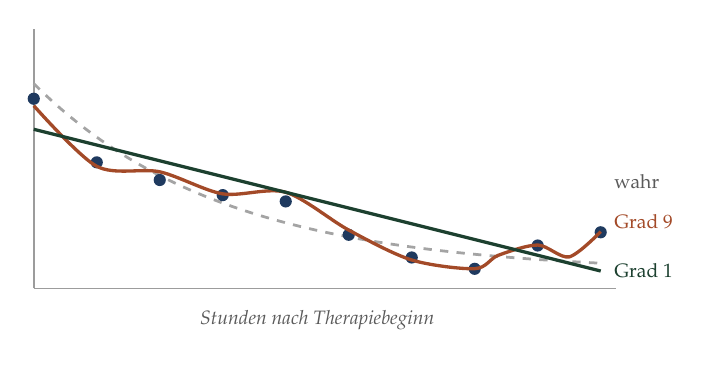
\begin{tikzpicture}[scale=1.0]
\draw[grau!60, line width=0.6pt] (0,0) -- (7.4,0);
\draw[grau!60, line width=0.6pt] (0,0) -- (0,3.3);
\draw[grau!55, line width=1.0pt, dashed, smooth, samples=60, domain=0:7.2]
  plot ({\x}, {0.8*(1+3*exp(-\x/2.4))-0.6});
\foreach \t/\y in {0.0/3.76,0.8/2.75,1.6/2.47,2.4/2.23,3.2/2.13,4.0/1.60,4.8/1.24,5.6/1.06,6.4/1.43,7.2/1.64}
  \fill[tief] (\t,{0.8*\y-0.6}) circle (2.2pt);
\draw[akzent, line width=1.2pt, smooth] plot coordinates {(0,2.32) (0.8,1.55) (1.6,1.48) (2.4,1.20) (3.2,1.22) (4.0,0.74) (4.8,0.36) (5.6,0.25) (5.9,0.42) (6.4,0.55) (6.8,0.4) (7.2,0.72)};
\draw[gruen!60!black, line width=1.2pt] (0,2.02) -- (7.2,0.22);
\node[font=\scriptsize, color=gruen!60!black, anchor=west] at (7.25,0.22) {Grad 1};
\node[font=\scriptsize, color=akzent, anchor=west] at (7.25,0.85) {Grad 9};
\node[font=\scriptsize, color=grau, anchor=west] at (7.25,1.35) {wahr};
\node[font=\scriptsize\itshape, color=grau] at (3.6,-0.4) {Stunden nach Therapiebeginn};
\end{tikzpicture}
\end{center}

\begin{center}
{\small
\renewcommand{\arraystretch}{1.5}
\begin{tabular}{@{}P{1.6cm}P{2.6cm}P{2.6cm}@{}}
\toprule
\textbf{Grad} & \textbf{Trainingsfehler} & \textbf{bei $t=11$}\\
\midrule
$1$ & $0{,}144$ & $1{,}15$\\
$3$ & $0{,}034$ & $1{,}40$\\
$9$ & $\mathbf{0{,}000}$ & $\mathbf{1{,}83}$\\
\midrule
wahr & --- & $1{,}19$\\
\bottomrule
\end{tabular}}
\end{center}

\begin{center}
\begin{minipage}{0.9\textwidth}
\textbf{Das Polynom neunten Grades läuft durch jeden Messpunkt --- und liegt bei $t=11$ am weitesten daneben.}
\end{minipage}
\end{center}

\begin{center}
\begin{minipage}{0.88\textwidth}
\kursiv{Zehn Punkte legen ein Polynom neunten Grades eindeutig fest; der Trainingsfehler ist also zwangsläufig null. \textbf{Die Kurve folgt dem Messrauschen} --- dem Ausreißer bei $10{,}7$ Stunden ebenso wie dem echten Verlauf --- und schwingt zwischen den Punkten aus. Das ist Aufgabe 1.3 in stetiger Form: Sie hat die Daten gelernt, nicht den Zusammenhang.}
\end{minipage}
\end{center}
\end{merksatz}

\section{Die Zerlegung}

\begin{merksatz}
\boxtitel{Worin ein Vorhersagefehler besteht}
Man denke sich viele Kliniken, die jede ihre eigenen zehn Messungen machen und jede ihr eigenes Polynom anpassen. An einer festen Stelle $x$ gibt jede eine andere Vorhersage $\hat h(x)$ ab.

\schritt{Drei Größen}
\begin{center}
{\small
\renewcommand{\arraystretch}{1.55}
\begin{tabular}{@{}P{2.4cm}P{6.2cm}@{}}
\toprule
\textbf{Rauschen} & $\sigma^{2}$ --- der Messfehler, den kein Verfahren beseitigt.\\
\textbf{Verzerrung} & $\bigl(\E[\hat h(x)] - f(x)\bigr)^{2}$ --- wie weit die \kursiv{mittlere} Vorhersage vom wahren Wert abliegt.\\
\textbf{Varianz} & $\E\bigl[(\hat h(x) - \E[\hat h(x)])^{2}\bigr]$ --- wie stark die Vorhersagen der Kliniken untereinander schwanken.\\
\bottomrule
\end{tabular}}
\end{center}
\end{merksatz}

\begin{merksatz}
\boxtitel{Satz 2.1 --- Verzerrung und Varianz}
Sei $y = f(x) + \varepsilon$ mit $\E[\varepsilon] = 0$ und $\operatorname{Var}[\varepsilon] = \sigma^{2}$, und sei $\varepsilon$ unabhängig von den Trainingsdaten. Dann gilt
\[ \E\bigl[(y - \hat h(x))^{2}\bigr] = \sigma^{2} + \bigl(\E[\hat h(x)] - f(x)\bigr)^{2} + \operatorname{Var}\bigl[\hat h(x)\bigr] . \]

\schritt{Beweis}
Schreibe $\bar h = \E[\hat h(x)]$ und zerlege
\[ y - \hat h = \underbrace{(y-f)}_{\varepsilon} + \underbrace{(f-\bar h)}_{\text{fest}} + \underbrace{(\bar h-\hat h)}_{\text{Schwankung}} . \]

\kursiv{Quadrieren} liefert drei Quadrate und drei gemischte Glieder. Die gemischten Glieder verschwinden im Erwartungswert:

\begin{center}
{\small
\renewcommand{\arraystretch}{1.5}
\begin{tabular}{@{}P{3.0cm}P{5.6cm}@{}}
\toprule
$2\,\varepsilon\,(f-\bar h)$ & $\E[\varepsilon] = 0$, der andere Faktor ist fest.\\
$2\,\varepsilon\,(\bar h-\hat h)$ & $\varepsilon$ unabhängig von den Daten, $\E[\varepsilon]=0$.\\
$2\,(f-\bar h)(\bar h-\hat h)$ & $\E[\bar h-\hat h] = \bar h - \bar h = 0$.\\
\bottomrule
\end{tabular}}
\end{center}

Es bleiben die drei Quadrate:
\[ \E[\varepsilon^{2}] + (f-\bar h)^{2} + \E[(\bar h-\hat h)^{2}] = \sigma^{2} + \text{Verzerrung}^{2} + \text{Varianz} \]
$\blacksquare$

\begin{center}
\begin{minipage}{0.9\textwidth}
\textbf{Der Fehler auf neuen Daten besteht aus drei Teilen --- und nur zwei davon hängen vom Verfahren ab.}
\end{minipage}
\end{center}
\end{merksatz}

\begin{merksatz}
\boxtitel{Der Leitfall zerlegt}
Viertausend simulierte Kliniken, je zehn Messungen, Fehler gemittelt über den ganzen Zeitraum:

\begin{center}
{\small
\renewcommand{\arraystretch}{1.44}
\begin{tabular}{@{}P{1.2cm}P{1.8cm}P{1.8cm}P{1.8cm}P{1.8cm}@{}}
\toprule
\textbf{Grad} & \textbf{Training} & \textbf{Verzerr.$^{2}$} & \textbf{Varianz} & \textbf{Test}\\
\midrule
$0$ & $0{,}886$ & $0{,}606$ & $0{,}009$ & $0{,}705$\\
$1$ & $0{,}184$ & $0{,}081$ & $0{,}017$ & $0{,}187$\\
$\mathbf{2}$ & $0{,}070$ & $0{,}005$ & $0{,}023$ & $\mathbf{0{,}119}$\\
$3$ & $0{,}054$ & $0{,}000$ & $0{,}031$ & $0{,}121$\\
$5$ & $0{,}035$ & $0{,}000$ & $0{,}047$ & $0{,}137$\\
$7$ & $0{,}019$ & $0{,}000$ & $0{,}080$ & $0{,}170$\\
$9$ & $0{,}000$ & $0{,}000$ & $0{,}595$ & $0{,}685$\\
\bottomrule
\end{tabular}}
\end{center}
\kursiv{Die Spalte \enquote{Test} ist $\sigma^{2} + \text{Verzerrung}^{2} + \text{Varianz}$ mit $\sigma^{2} = 0{,}09$.}

\begin{center}
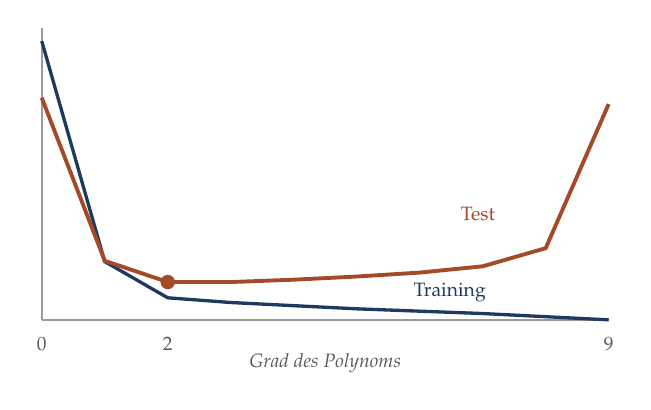
\begin{tikzpicture}[scale=1.0]
\draw[grau!60, line width=0.6pt] (0,0) -- (7.2,0);
\draw[grau!60, line width=0.6pt] (0,0) -- (0,3.7);
\draw[tief, line width=1.2pt] plot coordinates {(0,3.54) (0.8,0.74) (1.6,0.28) (2.4,0.22) (3.2,0.18) (4.0,0.14) (4.8,0.11) (5.6,0.08) (6.4,0.04) (7.2,0.0)};
\draw[akzent, line width=1.4pt] plot coordinates {(0,2.82) (0.8,0.75) (1.6,0.48) (2.4,0.48) (3.2,0.51) (4.0,0.55) (4.8,0.60) (5.6,0.68) (6.4,0.91) (7.2,2.74)};
\fill[akzent] (1.6,0.48) circle (2.6pt);
\node[font=\scriptsize, color=tief, anchor=west] at (4.6,0.35) {Training};
\node[font=\scriptsize, color=akzent, anchor=west] at (5.2,1.35) {Test};
\node[font=\scriptsize, color=grau, anchor=north] at (0,-0.1) {$0$};
\node[font=\scriptsize, color=grau, anchor=north] at (1.6,-0.1) {$2$};
\node[font=\scriptsize, color=grau, anchor=north] at (7.2,-0.1) {$9$};
\node[font=\scriptsize\itshape, color=grau] at (3.6,-0.55) {Grad des Polynoms};
\end{tikzpicture}
\end{center}

\begin{center}
\begin{minipage}{0.9\textwidth}
\textbf{Der Trainingsfehler fällt stetig. Der Testfehler fällt, erreicht bei Grad 2 sein Minimum und steigt wieder.}
\end{minipage}
\end{center}

\schritt{Was man ablesen kann}
\begin{center}
{\small
\renewcommand{\arraystretch}{1.5}
\begin{tabular}{@{}P{2.6cm}P{6.0cm}@{}}
\toprule
\textbf{Grad 0 und 1} & \Begriff{Unteranpassung}: Das Modell ist zu starr, um den Verlauf abzubilden. Die Verzerrung überwiegt.\\
\textbf{Grad 2 und 3} & Beide Anteile klein --- der beste Kompromiss.\\
\textbf{Grad 7 bis 9} & \Begriff{Überanpassung}: Das Modell folgt dem Rauschen. Die Varianz überwiegt.\\
\bottomrule
\end{tabular}}
\end{center}

\begin{center}
\begin{minipage}{0.88\textwidth}
\kursiv{\textbf{Grad 9 ist fast so schlecht wie Grad 0} --- $0{,}685$ gegen $0{,}705$. Wer alles lernt, ist kaum besser dran als wer nichts lernt, und aus genau demselben Grund wie in Aufgabe 1.3. Bemerkenswert ist auch, dass die wahre Kurve gar kein Polynom ist; kein Grad erreicht die Verzerrung null exakt, aber ab Grad 3 ist sie vernachlässigbar.}
\end{minipage}
\end{center}
\end{merksatz}

\section{Wie optimistisch der Trainingsfehler ist}

\begin{merksatz}
\boxtitel{Satz 2.2 --- der Optimismus}
Werden $p$ Parameter nach kleinsten Quadraten an $n$ Messpunkte angepasst und an \kursiv{denselben} Punkten mit neuen Messungen geprüft, so gilt
\[ \E[\text{Testfehler}] - \E[\text{Trainingsfehler}] = \frac{2\,\sigma^{2}\,p}{n} . \]

\schritt{Beweis}
Die Anpassung ist eine lineare Abbildung der Messwerte: $\hat{\vek y} = H\vek y$ mit der Projektionsmatrix $H$ auf den Raum der Polynome vom Grad $p-1$ (Band 2, Kapitel~9).

\kursiv{Erstens:} Der Unterschied zwischen einer neuen Messung $y_i'$ und der alten $y_i$ ist nur das Rauschen. Also
\[ \E\bigl[(y_i'-\hat y_i)^{2}\bigr] - \E\bigl[(y_i-\hat y_i)^{2}\bigr] = 2\operatorname{Cov}(\hat y_i,\,y_i) , \]
denn $y_i'$ ist von $\hat y_i$ unabhängig, $y_i$ aber nicht.

\kursiv{Zweitens:} Da $\hat{\vek y} = H\vek y$ und die Messfehler unabhängig mit Varianz $\sigma^{2}$ sind,
\[ \operatorname{Cov}(\hat y_i,\, y_i) = H_{ii}\,\sigma^{2} . \]

\kursiv{Drittens:} Die Spur einer Projektion ist die Dimension ihres Bildes:
\[ \sum_i H_{ii} = \operatorname{Spur} H = p . \]

\kursiv{Summieren und durch $n$ teilen:}
\[ \frac1n\sum_i 2\,H_{ii}\,\sigma^{2} = \frac{2\,\sigma^{2}\,p}{n} \]
$\blacksquare$

\schritt{Die Probe durch Simulation}
\begin{center}
{\small
\renewcommand{\arraystretch}{1.46}
\begin{tabular}{@{}P{1.2cm}P{1.2cm}P{2.4cm}P{2.4cm}@{}}
\toprule
$n$ & $p$ & \textbf{gemessen} & $2\sigma^{2}p/n$\\
\midrule
$10$ & $2$ & $0{,}0366$ & $0{,}0360$\\
$10$ & $3$ & $0{,}0542$ & $0{,}0540$\\
$10$ & $6$ & $0{,}1072$ & $0{,}1080$\\
$10$ & $10$ & $0{,}1807$ & $0{,}1800$\\
$30$ & $6$ & $0{,}0363$ & $0{,}0360$\\
\bottomrule
\end{tabular}}
\end{center}

\begin{center}
\begin{minipage}{0.9\textwidth}
\textbf{Der Trainingsfehler ist um einen Betrag zu optimistisch, der mit der Zahl der Parameter wächst und mit der Zahl der Beobachtungen fällt.}
\end{minipage}
\end{center}

\begin{center}
\begin{minipage}{0.88\textwidth}
\kursiv{Das ist die Grundlage aller Korrekturen, die man dem Trainingsfehler hinzufügt, um den Testfehler zu schätzen --- das Akaike-Kriterium aus Band 17 ist genau diese Rechnung in anderer Einheit. \textbf{Man \enquote{bezahlt} jeden Parameter mit $2\sigma^{2}/n$.} Kapitel~3 benutzt das, und Kapitel~7 verallgemeinert es auf Verfahren, bei denen man die Parameter nicht zählen kann.}
\end{minipage}
\end{center}

\schritt{Ein Vorbehalt}
\begin{center}
\begin{minipage}{0.88\textwidth}
\kursiv{Der Satz gilt an den Messpunkten selbst. \textbf{Zwischen den Messpunkten kann es erheblich schlimmer sein}: Beim Polynom neunten Grades beträgt der Optimismus an den Punkten $0{,}18$, über den ganzen Zeitraum aber $0{,}685$ --- die Kurve schwingt zwischen den Punkten aus, wo sie nie geprüft wurde. Das ist die zweite Warnung des Vorworts in quantitativer Gestalt.}
\end{minipage}
\end{center}
\end{merksatz}

\section{Mehr Daten}

\begin{merksatz}
\boxtitel{Was mit wachsendem $n$ geschieht}
\begin{center}
{\small
\renewcommand{\arraystretch}{1.46}
\begin{tabular}{@{}P{1.4cm}P{1.6cm}P{1.6cm}P{0.4cm}P{1.6cm}P{1.6cm}@{}}
\toprule
& \multicolumn{2}{c}{\textbf{Grad 2}} & & \multicolumn{2}{c}{\textbf{Grad 9}}\\
$n$ & Verzerr.$^{2}$ & Test & & Varianz & Test\\
\midrule
$10$ & $0{,}005$ & $0{,}118$ & & $0{,}589$ & $0{,}679$\\
$20$ & $0{,}005$ & $0{,}108$ & & $0{,}042$ & $0{,}132$\\
$50$ & $0{,}005$ & $0{,}100$ & & $0{,}017$ & $0{,}107$\\
$100$ & $0{,}004$ & $0{,}097$ & & $0{,}009$ & $0{,}099$\\
\bottomrule
\end{tabular}}
\end{center}

\begin{center}
\begin{minipage}{0.9\textwidth}
\textbf{Mehr Daten senken die Varianz, nicht die Verzerrung.}
\end{minipage}
\end{center}

\begin{center}
\begin{minipage}{0.88\textwidth}
\kursiv{Beim Polynom zweiten Grades bleibt eine Verzerrung von $0{,}004$ bestehen, gleich wie viele Messungen man hat --- die wahre Kurve ist eben keine Parabel. Beim Polynom neunten Grades verschwindet die Varianz, und bei hundert Messungen sind beide fast gleichauf. \textbf{Die richtige Komplexität hängt also von der Datenmenge ab}: Wer wenige Daten hat, muss sich bescheiden; wer viele hat, darf mehr wagen.}
\end{minipage}
\end{center}
\end{merksatz}

\section{Der Bruchfall}

\begin{warnung}
\boxtitelr{Was die Zerlegung voraussetzt}
\begin{center}
{\small
\renewcommand{\arraystretch}{1.52}
\begin{tabular}{@{}P{2.4cm}P{6.2cm}@{}}
\toprule
\textbf{Quadratischer Verlust} & Für den Null-Eins-Verlust aus Kapitel~1 gibt es keine so saubere Zerlegung.\\
\textbf{Festes Rauschen} & $\sigma^{2}$ ist überall gleich. Bei hohem Laktat ist die Messung oft ungenauer.\\
\textbf{Innerhalb des Bereichs} & Geprüft wird zwischen $0$ und $12$ Stunden. Außerhalb gilt nichts.\\
\bottomrule
\end{tabular}}
\end{center}

\schritt{Zur dritten Zeile}
Man frage das Polynom neunten Grades nach dem Wert bei $t = 14$ Stunden.

\begin{center}
\begin{minipage}{0.88\textwidth}
\kursiv{Es liefert eine Zahl, und die Zahl ist absurd --- bei der obigen Messreihe fällt die Kurve jenseits von zwölf Stunden steil ab oder steigt steil an, je nach Vorzeichen des höchsten Koeffizienten. \textbf{Auch das Polynom zweiten Grades wird außerhalb des Bereichs falsch}: Eine Parabel steigt irgendwann wieder, das Laktat nicht. Kein Satz dieses Kapitels sagt etwas über Vorhersagen außerhalb des Bereichs, in dem gemessen wurde.}
\end{minipage}
\end{center}

\schritt{Und ein Wort zum Leitfall}
\begin{center}
\begin{minipage}{0.88\textwidth}
\kursiv{Die zehn Messungen stammen von \kursiv{einem} Patienten. Wer aus ihnen eine Kurve für \kursiv{alle} Patienten ableitet, begeht einen Fehler, den keine Zerlegung erfasst: \textbf{Die Streuung zwischen Patienten ist eine andere Größe als die zwischen Messungen}, und sie ist meist die größere. Band 17, Kapitel~12 behandelt die Modelle, die beides trennen.}
\end{minipage}
\end{center}
\end{warnung}

\section{Übungsaufgaben}

\begin{aufgabe}
\boxtitel{Aufgabe 2.1 --- Die Zerlegung für den Mittelwert}
Man schätzt einen Laktatwert $\mu$ durch den Mittelwert $\bar y$ von $n$ Messungen mit Streuung $\sigma$. Zerlegen Sie den Fehler.

\loesung
\schritt{Schritt 1 --- Die Verzerrung}
\[ \E[\bar y] = \frac1n\sum_{i=1}^{n}\E[y_i] = \frac1n\cdot n\,\mu = \mu \]
\[ \text{Verzerrung} = \E[\bar y] - \mu = 0 \]

\schritt{Schritt 2 --- Die Varianz}
Bei unabhängigen Messungen addieren sich die Varianzen (Band 4, Kapitel~8):
\[ \operatorname{Var}[\bar y] = \frac{1}{n^{2}}\sum_{i=1}^{n}\operatorname{Var}[y_i] = \frac{1}{n^{2}}\cdot n\,\sigma^{2} = \frac{\sigma^{2}}{n} \]

\schritt{Schritt 3 --- Der Gesamtfehler für eine neue Messung}
\[ \E[(y-\bar y)^{2}] = \sigma^{2} + 0 + \frac{\sigma^{2}}{n} = \sigma^{2}\left(1+\frac1n\right) \]

\schritt{Schritt 4 --- Die Probe am Leitfall}
Grad 0 ist genau der Mittelwert. Mit $\sigma^{2} = 0{,}09$ und $n = 10$:
\[ \operatorname{Var} = \frac{0{,}09}{10} = 0{,}009 \]
Die Simulation ergab $0{,}009$. \checkmark

\begin{center}
\begin{minipage}{0.88\textwidth}
\kursiv{\textbf{Der Mittelwert ist unverzerrt --- und trotzdem das schlechteste Verfahren der Tabelle}, weil er den Verlauf gar nicht abbildet. Unverzerrtheit ist eine Eigenschaft bezüglich der Größe, die man schätzt; hier schätzt er eine Konstante, während die Wirklichkeit eine Kurve ist. Die Verzerrung von $0{,}606$ ist keine Verzerrung des Schätzers, sondern des Modells.}
\end{minipage}
\end{center}
\end{aufgabe}

\begin{aufgabe}
\boxtitel{Aufgabe 2.2 --- Absichtlich verzerren}
Ein Laktatwert $\mu = 1{,}2$ wird aus einer einzigen Messung mit Streuung $\sigma = 1$ geschätzt. Man verwendet statt $y$ den geschrumpften Schätzer $c\,y$ mit $0 < c \le 1$. Welches $c$ ist das beste?

\loesung
\schritt{Schritt 1 --- Verzerrung und Varianz}
\[ \E[c\,y] = c\,\mu \quad\Longrightarrow\quad \text{Verzerrung} = (c-1)\,\mu \]
\[ \operatorname{Var}[c\,y] = c^{2}\sigma^{2} \]

\schritt{Schritt 2 --- Der mittlere quadratische Fehler}
\[ M(c) = (c-1)^{2}\mu^{2} + c^{2}\sigma^{2} \]

\schritt{Schritt 3 --- Das Minimum}
\[ M'(c) = 2(c-1)\mu^{2} + 2c\,\sigma^{2} = 0 \]
\[ c\,(\mu^{2}+\sigma^{2}) = \mu^{2} \quad\Longrightarrow\quad c^{*} = \frac{\mu^{2}}{\mu^{2}+\sigma^{2}} \]

\kursiv{Im Beispiel:} $c^{*} = \frac{1{,}44}{1{,}44+1} = \frac{1{,}44}{2{,}44} = 0{,}590$.

\schritt{Schritt 4 --- Die Zahlen}
\begin{center}
{\small
\renewcommand{\arraystretch}{1.48}
\begin{tabular}{@{}P{1.6cm}P{2.0cm}P{1.8cm}P{1.8cm}@{}}
\toprule
$c$ & \textbf{Verzerr.$^{2}$} & \textbf{Varianz} & \textbf{Fehler}\\
\midrule
$1{,}000$ & $0{,}000$ & $1{,}000$ & $1{,}000$\\
$0{,}800$ & $0{,}058$ & $0{,}640$ & $0{,}698$\\
$\mathbf{0{,}590}$ & $0{,}242$ & $0{,}348$ & $\mathbf{0{,}590}$\\
$0{,}400$ & $0{,}518$ & $0{,}160$ & $0{,}678$\\
\bottomrule
\end{tabular}}
\end{center}

\begin{center}
\begin{minipage}{0.9\textwidth}
\textbf{Ein absichtlich verzerrter Schätzer hat einen um vierzig Prozent kleineren Fehler als der unverzerrte.}
\end{minipage}
\end{center}

\schritt{Schritt 5 --- Der Haken}
\begin{center}
\begin{minipage}{0.88\textwidth}
\kursiv{Das beste $c$ hängt von $\mu$ ab --- also von genau der Größe, die man schätzen will. \textbf{Man kann es nicht direkt benutzen.} Aber man sieht, in welche Richtung es geht: Bei großem Rauschen im Verhältnis zum Signal soll man stärker schrumpfen. Kapitel~4 macht daraus ein Verfahren, das mit einer aus den Daten geschätzten Stärke arbeitet --- die Regularisierung.}
\end{minipage}
\end{center}

\schritt{Schritt 6 --- Die Einordnung}
\begin{center}
\begin{minipage}{0.88\textwidth}
\kursiv{In Band 17 galt Unverzerrtheit als Tugend eines Schätzers. \textbf{Hier zeigt sich, dass sie zu teuer sein kann}: Wer um jeden Preis unverzerrt schätzt, zahlt mit Varianz. Das Lernen gibt diese Tugend bewusst auf --- und das ist einer der wenigen Punkte, an denen es der klassischen Statistik tatsächlich widerspricht.}
\end{minipage}
\end{center}
\end{aufgabe}

\begin{aufgabe}
\boxtitel{Aufgabe 2.3 --- Wie viele Messungen reichen?}
Nach Satz 2.2: Wie viele Messungen braucht man, damit der Optimismus eines Polynoms vierten Grades höchstens $0{,}02$ beträgt? ($\sigma = 0{,}3$.)

\loesung
\schritt{Schritt 1 --- Die Parameterzahl}
Ein Polynom vierten Grades hat $p = 5$ Koeffizienten.

\schritt{Schritt 2 --- Die Bedingung}
\[ \frac{2\,\sigma^{2}\,p}{n} \ \le\ 0{,}02 \]
\[ \frac{2\cdot0{,}09\cdot5}{n} = \frac{0{,}9}{n} \ \le\ 0{,}02 \]
\[ n \ \ge\ \frac{0{,}9}{0{,}02} = 45 \]

\begin{center}
\begin{minipage}{0.9\textwidth}
\textbf{Fünfundvierzig Messungen --- also neun je Parameter.}
\end{minipage}
\end{center}

\schritt{Schritt 3 --- Die Faustregel}
\[ \frac{n}{p} \ \ge\ \frac{2\,\sigma^{2}}{\text{zulässiger Optimismus}} \]

\begin{center}
{\small
\renewcommand{\arraystretch}{1.48}
\begin{tabular}{@{}P{3.0cm}P{2.4cm}@{}}
\toprule
\textbf{zulässig} & $n/p$\\
\midrule
$0{,}05$ & $3{,}6$\\
$0{,}02$ & $9$\\
$0{,}01$ & $18$\\
\bottomrule
\end{tabular}}
\end{center}

\begin{center}
\begin{minipage}{0.88\textwidth}
\kursiv{In der klinischen Forschung gilt die Faustregel \enquote{zehn Ereignisse je Merkmal} für Vorhersagemodelle. \textbf{Hier sieht man, woher sie kommt} --- und dass sie nicht absolut ist, sondern vom Verhältnis von Rauschen zu zulässigem Fehler abhängt. Bei verrauschten Daten reichen zehn nicht; bei sehr genauen genügen weniger.}
\end{minipage}
\end{center}

\schritt{Schritt 4 --- Warum \enquote{Ereignisse} und nicht \enquote{Patienten}}
\begin{center}
\begin{minipage}{0.88\textwidth}
\kursiv{Bei einer seltenen Zielgröße --- zehn Prozent Sepsis --- trägt nur die kleinere Gruppe Information über den Unterschied. Tausend Patienten mit hundert Sepsisfällen sind für ein Modell mit zwanzig Merkmalen knapp: fünf Ereignisse je Merkmal. \textbf{Die wirksame Stichprobengröße ist die der seltenen Klasse}, und das wird in Studien regelmäßig übersehen.}
\end{minipage}
\end{center}
\end{aufgabe}

\begin{geschichte}
\boxtitelg{Ein Paradoxon, das niemand glauben wollte}
\Person{Charles Stein} (1920--2016) zeigte 1956, dass der Mittelwert nicht der beste Schätzer ist --- sobald man mindestens drei Größen gleichzeitig schätzt.

\begin{center}
\begin{minipage}{0.9\textwidth}
\kursiv{Schätzt man drei oder mehr unabhängige Mittelwerte, so gibt es einen Schätzer, der \kursiv{für jede} Wahl der wahren Werte einen kleineren Gesamtfehler hat als die einzelnen Mittelwerte: Man schrumpft alle zum gemeinsamen Durchschnitt hin. \textbf{Das gilt selbst dann, wenn die Größen nichts miteinander zu tun haben} --- etwa der Weizenpreis, die Zahl der Sepsisfälle und die Durchschnittsgröße von Schülern.}
\end{minipage}
\end{center}

\schritt{Die Aufnahme}
\begin{center}
\begin{minipage}{0.9\textwidth}
\kursiv{Das Ergebnis wurde zunächst für einen Fehler gehalten. \Person{Willard James} und Stein gaben 1961 den expliziten Schätzer an, der heute ihren Namen trägt. \textbf{Aufgabe 2.2 ist der eindimensionale Schatten davon} --- nur dass dort das Schrumpfen ein unbekanntes $\mu$ braucht, während James und Stein es aus den Daten selbst bestimmen, was erst ab drei Dimensionen gelingt.}
\end{minipage}
\end{center}

\schritt{Der Name}
Die Begriffe \enquote{Verzerrung} und \enquote{Varianz} sind alt; ihre Gegenüberstellung als Zielkonflikt des Lernens stammt von \Person{Stuart Geman}, \Person{Elie Bienenstock} und \Person{René Doursat} aus dem Jahr 1992.

\begin{center}
\begin{minipage}{0.9\textwidth}
\kursiv{Ihr Aufsatz handelte von neuronalen Netzen und war als Warnung gemeint: Große Netze hätten zu viel Varianz, um aus begrenzten Daten zu lernen. \textbf{Dreißig Jahre später ist das Bild verwickelter} --- Kapitel~14 zeigt, dass sehr große Netze die Kurve dieses Kapitels auf eine Weise verlassen, die niemand vorhergesagt hatte.}
\end{minipage}
\end{center}
\end{geschichte}

\begin{forschung}
\boxtitelp{Verzerrung und Varianz heute}
\begin{center}
{\small
\renewcommand{\arraystretch}{1.45}
\begin{tabular}{@{}P{2.8cm}P{5.4cm}@{}}
\toprule
\textbf{Doppelter Abstieg} & Jenseits der Interpolationsschwelle fällt der Testfehler wieder.\\
\textbf{Klinische Modelle} & Mindestgrößen für Vorhersagemodelle, die über die Zehnerregel hinausgehen.\\
\textbf{Ungleiche Streuung} & Modelle, die die Unsicherheit mitlernen.\\
\bottomrule
\end{tabular}}
\end{center}

\schritt{Zur ersten Zeile}
\begin{center}
\begin{minipage}{0.88\textwidth}
\kursiv{Die Tabelle dieses Kapitels endet bei Grad 9 --- genau dort, wo das Polynom die Daten interpoliert. \textbf{Was geschieht bei Grad 20 oder 100?} Die klassische Antwort lautet: noch schlimmer. Seit 2019 weiß man, dass unter bestimmten Umständen das Gegenteil eintritt: Der Testfehler erreicht an der Interpolationsschwelle ein Maximum und fällt danach wieder. Kapitel~14 behandelt das ausführlich.}
\end{minipage}
\end{center}

\schritt{Zur zweiten Zeile}
\begin{center}
\begin{minipage}{0.88\textwidth}
\kursiv{\Person{Richard Riley} und Mitarbeiter gaben ab 2019 Formeln für die Mindestgröße klinischer Vorhersagestudien an, die den Optimismus aus Satz 2.2 ausdrücklich begrenzen. \textbf{Sie ergeben oft deutlich mehr als zehn Ereignisse je Merkmal} --- und viele veröffentlichte Modelle erfüllen sie nicht.}
\end{minipage}
\end{center}
\end{forschung}

\begin{merksatz}
\boxtitel{Was Sie jetzt können}
\begin{center}
\renewcommand{\arraystretch}{1.5}
\begin{tabular}{@{}P{3.0cm}P{5.6cm}@{}}
\toprule
\textbf{Satz 2.1} & Fehler $=$ Rauschen $+$ Verzerrung$^{2}$ $+$ Varianz\\
\textbf{Unteranpassung} & zu starr, Verzerrung überwiegt\\
\textbf{Überanpassung} & zu frei, Varianz überwiegt\\
\textbf{Satz 2.2} & Optimismus $2\sigma^{2}p/n$\\
\textbf{Mehr Daten} & senken die Varianz, nicht die Verzerrung\\
\bottomrule
\end{tabular}
\end{center}

\begin{center}
\begin{minipage}{0.88\textwidth}
\kursiv{Im Leitfall kannten wir die wahre Kurve und konnten den Testfehler ausrechnen. Das nächste Kapitel fragt, wie man ihn schätzt, wenn man sie nicht kennt --- und wie man dabei betrügt, ohne es zu merken.}
\end{minipage}
\end{center}
\end{merksatz}

\chapter{Wie man prüft --- und wie man sich betrügt}

\section{Der Leitfall}

\begin{merksatz}
\boxtitel{Ein Modell mit vielen Merkmalen}
Das Klinikum hat inzwischen mehr als Laktat. Für $50$ Patienten der Intensivstation liegen $5000$ Laborwerte, Genexpressionsdaten und Vitalparameter vor; $25$ entwickelten eine Sepsis, $25$ nicht.

\begin{center}
\begin{minipage}{0.9\textwidth}
\textbf{Die Frage:} Wie gut wird ein daraus gelerntes Modell bei den nächsten Patienten sein?
\end{minipage}
\end{center}

\begin{center}
\begin{minipage}{0.88\textwidth}
\kursiv{In Kapitel~2 konnten wir den Testfehler ausrechnen, weil wir die wahre Kurve kannten. \textbf{Jetzt kennen wir sie nicht}, und der Trainingsfehler ist nach Satz 2.2 zu optimistisch --- bei $5000$ Merkmalen und $50$ Patienten sogar grotesk. Wir brauchen Daten, die das Modell nicht gesehen hat.}
\end{minipage}
\end{center}
\end{merksatz}

\section{Zurückhalten}

\begin{merksatz}
\boxtitel{Die drei Teile}
\begin{center}
{\small
\renewcommand{\arraystretch}{1.55}
\begin{tabular}{@{}P{2.4cm}P{6.2cm}@{}}
\toprule
\textbf{Training} & Daraus lernt das Verfahren.\\
\textbf{Validierung} & Damit wählt man zwischen Verfahren oder Einstellungen --- etwa dem Grad des Polynoms.\\
\textbf{Test} & Wird genau einmal benutzt, ganz am Ende, um den Fehler des gewählten Verfahrens zu schätzen.\\
\bottomrule
\end{tabular}}
\end{center}

\begin{center}
\begin{minipage}{0.9\textwidth}
\textbf{Wer die Testdaten zum Auswählen benutzt, hat keine Testdaten mehr.}
\end{minipage}
\end{center}

\begin{center}
\begin{minipage}{0.88\textwidth}
\kursiv{Das ist die wichtigste Regel dieses Kapitels. \textbf{Jede Entscheidung, die man aufgrund der Testdaten trifft, macht sie zu Trainingsdaten} --- und ihr Fehler wird so optimistisch wie der Trainingsfehler. Wer zwanzig Modelle auf denselben Testdaten vergleicht und das beste berichtet, berichtet den Fehler des besten von zwanzig Glücksfällen.}
\end{minipage}
\end{center}

\schritt{Das Problem bei kleinen Daten}
\begin{center}
\begin{minipage}{0.88\textwidth}
\kursiv{Bei $50$ Patienten bleiben nach der Aufteilung vielleicht $30$ zum Lernen und je $10$ für Validierung und Test. \textbf{Zehn Testpatienten geben einen Fehler auf zehn Prozentpunkte genau} --- kaum besser als eine Münze. Man braucht ein Verfahren, das die Daten mehrfach verwendet, ohne zu betrügen.}
\end{minipage}
\end{center}
\end{merksatz}

\begin{definition}
\boxtitelm{Definition 3.1 --- $k$-fache Kreuzvalidierung}
\begin{center}
{\small
\renewcommand{\arraystretch}{1.5}
\begin{tabular}{@{}P{1.0cm}P{7.4cm}@{}}
\toprule
$1$ & Teile die Daten zufällig in $k$ gleich große Teile.\\
$2$ & Für jeden Teil $j$: Lerne auf den übrigen $k-1$ Teilen, prüfe auf Teil $j$.\\
$3$ & Mittle die $k$ Prüffehler.\\
\bottomrule
\end{tabular}}
\end{center}
\end{definition}

\begin{merksatz}
\boxtitel{Was dabei geschieht}
\begin{center}
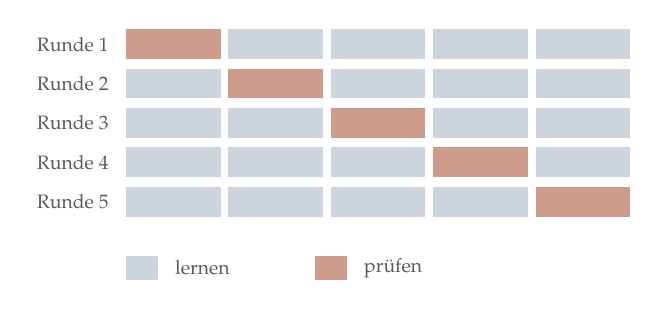
\begin{tikzpicture}[scale=1.0]
\foreach \r in {0,...,4} {
  \foreach \c in {0,...,4} {
    \ifnum\r=\c
      \fill[akzent!55] (\c*1.3,-\r*0.5) rectangle ++(1.2,0.38);
    \else
      \fill[tief!22] (\c*1.3,-\r*0.5) rectangle ++(1.2,0.38);
    \fi
  }
  \node[font=\scriptsize, color=grau, anchor=east] at (-0.1,{-\r*0.5+0.19}) {Runde \the\numexpr\r+1\relax};
}
\fill[tief!22] (0,-2.8) rectangle ++(0.4,0.3); \node[font=\scriptsize, color=grau, anchor=west] at (0.5,-2.65) {lernen};
\fill[akzent!55] (2.4,-2.8) rectangle ++(0.4,0.3); \node[font=\scriptsize, color=grau, anchor=west] at (2.9,-2.65) {prüfen};
\end{tikzpicture}
\end{center}

\begin{center}
\begin{minipage}{0.9\textwidth}
\textbf{Jeder Patient wird genau einmal geprüft --- und zwar von einem Modell, das ihn nicht gesehen hat.}
\end{minipage}
\end{center}

\schritt{Die Wahl von $k$}
\begin{center}
{\small
\renewcommand{\arraystretch}{1.5}
\begin{tabular}{@{}P{2.0cm}P{6.6cm}@{}}
\toprule
$k$ \textbf{klein} & Man lernt auf weniger Daten; der geschätzte Fehler ist etwas zu pessimistisch.\\
$k = n$ & \Begriff{Weglassen einzelner Fälle}: fast alle Daten zum Lernen, aber $n$ Modelle zu rechnen.\\
\textbf{üblich} & $k = 5$ oder $k = 10$ --- ein bewährter Kompromiss.\\
\bottomrule
\end{tabular}}
\end{center}

\schritt{Satz 3.2 --- die Abkürzung bei kleinsten Quadraten}
Beim Weglassen einzelner Fälle muss man das Modell nicht $n$-mal neu anpassen. Mit dem Residuum $e_i = y_i - \hat y_i$ des vollen Modells und dem Diagonalelement $H_{ii}$ der Projektion aus Satz 2.2 gilt
\[ y_i - \hat y_{(-i)} = \frac{e_i}{1-H_{ii}} . \]

\begin{center}
\begin{minipage}{0.88\textwidth}
\kursiv{Der Beweis braucht eine Formel für die Inverse einer Matrix nach einer Änderung vom Rang eins; wir verzichten auf ihn --- die erste Auslassung dieses Bandes. \textbf{Aufgabe 3.2 prüft den Satz am einfachsten Fall nach}, dem Mittelwert, wo er sich in drei Zeilen herleiten lässt. Man liest an ihm ab, warum Punkte mit großem $H_{ii}$ --- \enquote{Hebelpunkte} am Rand des Messbereichs --- beim Weglassen besonders stark ausschlagen.}
\end{minipage}
\end{center}
\end{merksatz}

\section{Das Leck}

\begin{warnung}
\boxtitelr{Ein Versuch mit reinem Zufall}
Man nehme den Leitfall --- aber mit Daten, die \kursiv{keinerlei} Information enthalten: $5000$ Zufallszahlen je Patient, unabhängig davon, ob er eine Sepsis hat.

\begin{center}
\begin{minipage}{0.9\textwidth}
\textbf{Der wahre Fehler jedes Verfahrens beträgt fünfzig Prozent.} Mehr als Raten ist nicht möglich.
\end{minipage}
\end{center}

\schritt{Das Vorgehen, falsch}
\begin{center}
{\small
\renewcommand{\arraystretch}{1.5}
\begin{tabular}{@{}P{1.0cm}P{7.4cm}@{}}
\toprule
$1$ & Wähle aus den $5000$ Merkmalen die $100$, die mit der Sepsis am stärksten zusammenhängen --- auf \textcolor{akzent}{allen} $50$ Patienten.\\
$2$ & Führe mit diesen $100$ Merkmalen eine fünffache Kreuzvalidierung durch.\\
\bottomrule
\end{tabular}}
\end{center}

\schritt{Das Vorgehen, richtig}
\begin{center}
{\small
\renewcommand{\arraystretch}{1.5}
\begin{tabular}{@{}P{1.0cm}P{7.4cm}@{}}
\toprule
$1$ & Führe eine fünffache Kreuzvalidierung durch.\\
$2$ & Wähle in \textcolor{gruen}{jeder Runde} die $100$ Merkmale nur auf den Lerndaten dieser Runde.\\
\bottomrule
\end{tabular}}
\end{center}

\schritt{Das Ergebnis, fünfzigmal wiederholt}
\begin{center}
{\small
\renewcommand{\arraystretch}{1.5}
\begin{tabular}{@{}P{3.0cm}P{2.6cm}P{2.4cm}@{}}
\toprule
\textbf{Vorgehen} & \textbf{geschätzter Fehler} & \textbf{wahr}\\
\midrule
falsch & $\mathbf{1{,}5\,\%}$ & $50\,\%$\\
richtig & $53{,}5\,\%$ & $50\,\%$\\
\bottomrule
\end{tabular}}
\end{center}

\begin{center}
\begin{minipage}{0.9\textwidth}
\textbf{Aus reinem Rauschen wird ein Modell mit $98{,}5$ Prozent Treffsicherheit.}
\end{minipage}
\end{center}
\end{warnung}

\begin{merksatz}
\boxtitel{Woher das kommt}
Bei $5000$ Zufallsmerkmalen und $50$ Patienten hängt das zufällig stärkste Merkmal deutlich mit der Zielgröße zusammen.

\schritt{Die höchste Zufallskorrelation}
Näherungsweise gilt für $m$ unabhängige Merkmale und $n$ Beobachtungen
\[ \max_j\,|r_j| \ \approx\ \sqrt{\frac{2\ln m}{n}} . \]

\begin{center}
{\small
\renewcommand{\arraystretch}{1.46}
\begin{tabular}{@{}P{2.0cm}P{2.4cm}@{}}
\toprule
$m$ & $\max|r|$\\
\midrule
$10$ & $0{,}30$\\
$100$ & $0{,}43$\\
$1000$ & $0{,}53$\\
$5000$ & $0{,}58$\\
\bottomrule
\end{tabular}}
\end{center}
\kursiv{Für $n=50$. Die Simulation ergibt bei $m = 5000$ im Mittel $0{,}52$ --- die Näherung liegt etwas zu hoch, die Größenordnung stimmt.}

\begin{center}
\begin{minipage}{0.88\textwidth}
\kursiv{Eine Korrelation von $0{,}5$ gilt in der Medizin als stark. \textbf{Hier ist sie reiner Zufall}, und die Auswahl der hundert besten Merkmale hat genau diese Zufälle eingesammelt --- auch die Zufälle in den Patienten, die später als \enquote{Prüfdaten} dienen. Die Kreuzvalidierung prüft danach nur noch, ob die Zufälle in sich stimmig sind. Sie sind es.}
\end{minipage}
\end{center}

\schritt{Die Regel}
\begin{center}
\begin{minipage}{0.9\textwidth}
\textbf{Alles, was aus den Daten gelernt wird --- auch Auswahl, Normierung, Auffüllen fehlender Werte ---, gehört \kursiv{in} die Kreuzvalidierung, nicht davor.}
\end{minipage}
\end{center}

\begin{center}
\begin{minipage}{0.88\textwidth}
\kursiv{\textbf{Dieser Fehler ist in veröffentlichten Arbeiten erschreckend häufig.} Eine Übersicht aus dem Jahr 2002 fand ihn in einer Reihe viel zitierter Studien zur Krebsdiagnose aus Genexpressionsdaten; die berichteten Fehlerraten nahe null waren durch das Leck erklärbar. Eine spätere Durchsicht über viele Fachgebiete hinweg fand Lecks in Hunderten von Arbeiten.}
\end{minipage}
\end{center}
\end{merksatz}

\section{Mehr als eine Fehlerrate}

\begin{merksatz}
\boxtitel{Die Trennschärfe}
Viele Verfahren liefern keine Ja-Nein-Antwort, sondern eine Zahl --- eine geschätzte Wahrscheinlichkeit. Erst eine Schwelle macht daraus eine Entscheidung, und Kapitel~1 zeigte, dass die Wahl der Schwelle eine eigene Frage ist.

\begin{definition}
\boxtitelm{Definition 3.3 --- Fläche unter der Kurve}
Die \Begriff{Trennschärfe} (englisch AUC) ist die Wahrscheinlichkeit, dass ein zufällig gewählter Sepsispatient eine höhere Zahl erhält als ein zufällig gewählter ohne Sepsis.
\end{definition}

\begin{center}
{\small
\renewcommand{\arraystretch}{1.5}
\begin{tabular}{@{}P{2.0cm}P{6.6cm}@{}}
\toprule
$0{,}5$ & Nicht besser als Raten.\\
$0{,}7$ & Brauchbar für grobe Einordnung.\\
$0{,}8$ & Gut.\\
$0{,}9$ & Sehr gut --- in der Medizin selten.\\
\bottomrule
\end{tabular}}
\end{center}

\begin{center}
\begin{minipage}{0.88\textwidth}
\kursiv{Der Name kommt daher, dass die Größe gleich der Fläche unter der Kurve ist, die Empfindlichkeit gegen Falsch-positiv-Rate für alle Schwellen aufträgt (Band 17, Kapitel~5). \textbf{Die obige Deutung als Paarvergleich ist anschaulicher} und für die Rechnung von Hand bequemer, wie Aufgabe 3.1 zeigt.}
\end{minipage}
\end{center}
\end{merksatz}

\begin{warnung}
\boxtitelr{Was die Trennschärfe nicht misst}
\begin{center}
{\small
\renewcommand{\arraystretch}{1.5}
\begin{tabular}{@{}P{2.8cm}P{5.8cm}@{}}
\toprule
\textbf{Kalibrierung} & Ob eine vorhergesagte Wahrscheinlichkeit von $30$ Prozent tatsächlich in $30$ Prozent der Fälle eintritt.\\
\textbf{Nutzen} & Ob die Warnung früh genug kommt, um etwas zu ändern.\\
\textbf{Übertrag\-barkeit} & Ob sie in einer anderen Klinik gleich hoch ist.\\
\bottomrule
\end{tabular}}
\end{center}

\begin{center}
\begin{minipage}{0.88\textwidth}
\kursiv{Die Trennschärfe hängt nicht von der Prävalenz ab --- sie vergleicht nur Paare. \textbf{Das ist zugleich ihr Vorzug und ihre Gefahr}: Wechselt ein Modell von der Intensiv- auf die Normalstation, kann die Trennschärfe gleich bleiben, während alle Wahrscheinlichkeiten um den Faktor fünf zu hoch liegen. Aufgabe 1.2 hat diesen Fall bereits gezeigt; eine Trennschärfe allein hätte ihn nicht bemerkt.}
\end{minipage}
\end{center}
\end{warnung}

\section{Die äußere Prüfung}

\begin{merksatz}
\boxtitel{Der Fall von 2021}
Ein kommerzielles Sepsis-Warnsystem, in Hunderten amerikanischer Krankenhäuser im Einsatz, wurde an einer Universitätsklinik unabhängig nachgeprüft --- an rund $38\,000$ stationären Aufenthalten.

\begin{center}
{\small
\renewcommand{\arraystretch}{1.5}
\begin{tabular}{@{}P{3.2cm}P{2.6cm}P{2.2cm}@{}}
\toprule
& \textbf{Hersteller} & \textbf{Nachprüfung}\\
\midrule
Trennschärfe & $0{,}76$--$0{,}83$ & $\mathbf{0{,}63}$\\
erkannte Sepsisfälle & --- & $33\,\%$\\
Warnung bei allen Aufenthalten & --- & $18\,\%$\\
\bottomrule
\end{tabular}}
\end{center}

\begin{center}
\begin{minipage}{0.9\textwidth}
\textbf{Das System warnte bei fast jedem fünften Patienten --- und übersah zwei von drei Sepsisfällen.}
\end{minipage}
\end{center}

\schritt{Warum die innere Prüfung das nicht zeigen konnte}
\begin{center}
{\small
\renewcommand{\arraystretch}{1.5}
\begin{tabular}{@{}P{2.4cm}P{6.2cm}@{}}
\toprule
\textbf{Andere Kranke} & Andere Klinik, andere Patientenmischung, andere Prävalenz.\\
\textbf{Andere Praxis} & Andere Zeitpunkte der Laborabnahme, andere Dokumentation.\\
\textbf{Andere Etiketten} & Was als Sepsis gezählt wurde, war nicht einheitlich definiert.\\
\bottomrule
\end{tabular}}
\end{center}

\begin{center}
\begin{minipage}{0.88\textwidth}
\kursiv{Keine Kreuzvalidierung kann das aufdecken, denn sie teilt dieselben Daten nur anders auf. \textbf{Sie beantwortet die Frage \enquote{wie gut auf Patienten wie diesen?} --- nicht \enquote{wie gut auf meinen Patienten?}} Dafür braucht man eine \Begriff{äußere Prüfung}: an Daten einer anderen Klinik, aus einer anderen Zeit, erhoben von anderen Leuten.}
\end{minipage}
\end{center}
\end{merksatz}

\section{Der Bruchfall}

\begin{warnung}
\boxtitelr{Das Leck in der Zeit}
Ein besonders heimtückischer Fall: Ein Merkmal steht in den Daten, das zum Zeitpunkt der Vorhersage noch gar nicht bekannt war.

\schritt{Ein Beispiel}
\begin{center}
{\small
\renewcommand{\arraystretch}{1.5}
\begin{tabular}{@{}P{3.0cm}P{5.6cm}@{}}
\toprule
\textbf{Merkmal} & \enquote{Blutkultur angeordnet}\\
\textbf{Zusammenhang} & sehr stark mit späterer Sepsisdiagnose\\
\textbf{Grund} & Der Arzt hatte die Sepsis bereits vermutet.\\
\bottomrule
\end{tabular}}
\end{center}

\begin{center}
\begin{minipage}{0.9\textwidth}
\textbf{Das Modell sagt voraus, was der Arzt schon wusste --- und rühmt sich dafür.}
\end{minipage}
\end{center}

\begin{center}
\begin{minipage}{0.88\textwidth}
\kursiv{Solche Merkmale ergeben hervorragende Trennschärfen und keinerlei Nutzen, denn die Warnung kommt nach dem Verdacht, den sie vorwegnehmen sollte. \textbf{Dieser Fehler ist in mehreren veröffentlichten Frühwarnmodellen nachgewiesen worden.} Die Abhilfe ist streng, aber einfach: Für jedes Merkmal muss feststehen, wann es im Behandlungsverlauf verfügbar wurde, und nur was vor dem Vorhersagezeitpunkt vorlag, darf verwendet werden.}
\end{minipage}
\end{center}

\schritt{Und das Leck über Patienten}
\begin{center}
\begin{minipage}{0.88\textwidth}
\kursiv{Hat ein Patient mehrere Aufenthalte, und landet einer im Training und einer im Test, so erkennt das Modell ihn wieder --- an Alter, Vorerkrankungen, Medikation. \textbf{Aufgeteilt werden muss nach Patienten, nicht nach Aufenthalten.} Bei Bilddaten gilt dasselbe für mehrere Aufnahmen derselben Person; das Versäumnis hat bei einigen frühen Arbeiten zur Hautkrebserkennung zu deutlich überhöhten Werten geführt.}
\end{minipage}
\end{center}
\end{warnung}

\section{Übungsaufgaben}

\begin{aufgabe}
\boxtitel{Aufgabe 3.1 --- Trennschärfe von Hand}
Ein Modell gibt zehn Patienten folgende Werte:
\begin{center}
{\small
\renewcommand{\arraystretch}{1.5}
\begin{tabular}{@{}P{2.4cm}P{5.6cm}@{}}
\toprule
\textbf{Sepsis} & $0{,}9$ \quad $0{,}7$ \quad $0{,}6$ \quad $0{,}3$\\
\textbf{keine} & $0{,}8$ \quad $0{,}5$ \quad $0{,}4$ \quad $0{,}2$ \quad $0{,}15$ \quad $0{,}1$\\
\bottomrule
\end{tabular}}
\end{center}

\loesung
\schritt{Schritt 1 --- Die Zahl der Paare}
\[ 4\cdot6 = 24 \]

\schritt{Schritt 2 --- Jeden Sepsispatienten mit allen anderen vergleichen}
\begin{center}
{\small
\renewcommand{\arraystretch}{1.48}
\begin{tabular}{@{}P{1.8cm}P{4.2cm}P{1.6cm}@{}}
\toprule
\textbf{Sepsis} & \textbf{höher als} & \textbf{Anzahl}\\
\midrule
$0{,}9$ & alle sechs & $6$\\
$0{,}7$ & alle außer $0{,}8$ & $5$\\
$0{,}6$ & alle außer $0{,}8$ & $5$\\
$0{,}3$ & $0{,}2$; $0{,}15$; $0{,}1$ & $3$\\
\midrule
\textbf{Summe} & & $\mathbf{19}$\\
\bottomrule
\end{tabular}}
\end{center}

\schritt{Schritt 3 --- Die Trennschärfe}
\[ \text{AUC} = \frac{19}{24} = 0{,}792 \]

\begin{center}
\begin{minipage}{0.9\textwidth}
\textbf{In knapp vier von fünf Paaren ordnet das Modell richtig.}
\end{minipage}
\end{center}

\schritt{Schritt 4 --- Eine Schwelle wählen}
\begin{center}
{\small
\renewcommand{\arraystretch}{1.46}
\begin{tabular}{@{}P{1.8cm}P{2.2cm}P{2.2cm}P{1.6cm}@{}}
\toprule
\textbf{Schwelle} & \textbf{Empfindl.} & \textbf{Fehlalarme} & \textbf{Fehler}\\
\midrule
$0{,}85$ & $1/4$ & $0/6$ & $3$\\
$0{,}55$ & $3/4$ & $1/6$ & $2$\\
$0{,}25$ & $4/4$ & $3/6$ & $3$\\
\bottomrule
\end{tabular}}
\end{center}

\begin{center}
\begin{minipage}{0.88\textwidth}
\kursiv{Dieselbe Trennschärfe von $0{,}792$ steht hinter allen drei Zeilen. \textbf{Die Trennschärfe beschreibt das Modell, nicht die Entscheidung} --- welche Zeile man wählt, hängt wieder von den Kosten ab. Bei Kosten $10:1$ ist die unterste die beste: $10\cdot0 + 3 = 3$ gegen $10\cdot1 + 1 = 11$ für die mittlere.}
\end{minipage}
\end{center}

\schritt{Schritt 5 --- Der Zusammenhang mit einem bekannten Test}
\begin{center}
\begin{minipage}{0.88\textwidth}
\kursiv{Die Zahl $19$ ist die Teststatistik des Mann-Whitney-Tests aus Band 17, Kapitel~9. \textbf{Trennschärfe und Rangtest sind dieselbe Größe}, einmal als Maß, einmal als Prüfgröße --- und daraus folgt auch, wie man ein Vertrauensintervall für die Trennschärfe gewinnt.}
\end{minipage}
\end{center}
\end{aufgabe}

\begin{aufgabe}
\boxtitel{Aufgabe 3.2 --- Weglassen beim Mittelwert}
Man sagt jeden Laktatwert durch den Mittelwert der übrigen vorher. Zeigen Sie, dass der Fehler beim Weglassen gleich $\frac{n}{n-1}(y_i-\bar y)$ ist, und prüfen Sie Satz 3.2.

\loesung
\schritt{Schritt 1 --- Der Mittelwert ohne $y_i$}
\[ \bar y_{(-i)} = \frac{n\,\bar y - y_i}{n-1} \]

\schritt{Schritt 2 --- Der Fehler}
\[ y_i - \bar y_{(-i)} = y_i - \frac{n\,\bar y - y_i}{n-1} = \frac{(n-1)\,y_i - n\,\bar y + y_i}{n-1} = \frac{n\,y_i - n\,\bar y}{n-1} \]
\[ = \frac{n}{n-1}\,(y_i-\bar y) \]

\schritt{Schritt 3 --- Satz 3.2 prüfen}
Beim Mittelwert ist $H$ die Matrix, deren Einträge alle $\tfrac1n$ sind --- jede Vorhersage ist der Durchschnitt aller Werte. Also $H_{ii} = \tfrac1n$:
\[ \frac{e_i}{1-H_{ii}} = \frac{y_i-\bar y}{1-\frac1n} = \frac{y_i-\bar y}{\frac{n-1}{n}} = \frac{n}{n-1}\,(y_i-\bar y) \quad \checkmark \]

\schritt{Schritt 4 --- Zahlen}
Laktatwerte $1{,}0$; $1{,}4$; $1{,}2$; $2{,}4$; $\bar y = 1{,}5$; $n = 4$.

\begin{center}
{\small
\renewcommand{\arraystretch}{1.48}
\begin{tabular}{@{}P{1.4cm}P{1.8cm}P{2.2cm}P{2.2cm}@{}}
\toprule
$y_i$ & $e_i$ & $\frac43\,e_i$ & \textbf{direkt}\\
\midrule
$1{,}0$ & $-0{,}5$ & $-0{,}667$ & $1{,}0-1{,}667$\\
$1{,}4$ & $-0{,}1$ & $-0{,}133$ & $1{,}4-1{,}533$\\
$1{,}2$ & $-0{,}3$ & $-0{,}400$ & $1{,}2-1{,}600$\\
$2{,}4$ & $+0{,}9$ & $+1{,}200$ & $2{,}4-1{,}200$\\
\bottomrule
\end{tabular}}
\end{center}

\kursiv{Probe letzte Zeile:} Mittelwert der übrigen $\frac{1{,}0+1{,}4+1{,}2}{3} = 1{,}2$; $2{,}4-1{,}2 = 1{,}2$. \checkmark

\schritt{Schritt 5 --- Der Vergleich}
\begin{center}
{\small
\renewcommand{\arraystretch}{1.5}
\begin{tabular}{@{}P{3.0cm}P{2.4cm}@{}}
\toprule
& \textbf{mittl.\ Quadrat}\\
\midrule
Trainingsfehler & $0{,}290$\\
Weglassen & $0{,}516$\\
\bottomrule
\end{tabular}}
\end{center}

\kursiv{Zur ersten Zeile:} $\frac14(0{,}25+0{,}01+0{,}09+0{,}81) = \frac{1{,}16}{4} = 0{,}290$.\\
\kursiv{Zur zweiten:} $\left(\frac43\right)^{2}\cdot0{,}290 = \frac{16}{9}\cdot0{,}290 = 0{,}516$.

\begin{center}
\begin{minipage}{0.88\textwidth}
\kursiv{\textbf{Beim Weglassen wird jeder Fehler um den Faktor $\frac{n}{n-1}$ größer} --- bei nur vier Werten um ein Drittel, im Quadrat um drei Viertel. Der Trainingsfehler unterschätzt hier um fast die Hälfte. Bei großem $n$ schrumpft der Unterschied; bei kleinem ist er die Regel.}
\end{minipage}
\end{center}
\end{aufgabe}

\begin{aufgabe}
\boxtitel{Aufgabe 3.3 --- Wie viele Modelle darf man vergleichen?}
Man vergleicht $20$ Modelle auf denselben $200$ Testpatienten. Alle sind in Wahrheit gleich gut, mit einer Trefferquote von $80$ Prozent. Welche Trefferquote hat das \enquote{beste}?

\loesung
\schritt{Schritt 1 --- Die Streuung eines einzelnen Testergebnisses}
Die gemessene Quote ist ein Anteil aus $200$ Versuchen:
\[ \sigma = \sqrt{\frac{0{,}8\cdot0{,}2}{200}} = \sqrt{0{,}0008} = 0{,}0283 \]

\schritt{Schritt 2 --- Das Beste von zwanzig}
Das Maximum von $20$ unabhängigen normalverteilten Größen liegt im Mittel etwa $1{,}87$ Standardabweichungen über dem Erwartungswert.

\kursiv{Der Wert $1{,}87$ ist der Erwartungswert des Maximums von $20$ Standardnormalverteilten; er lässt sich tabellieren oder simulieren.}

\schritt{Schritt 3 --- Die Rechnung}
\[ 0{,}80 + 1{,}87\cdot0{,}0283 = 0{,}80 + 0{,}053 = 0{,}853 \]

\begin{center}
\begin{minipage}{0.9\textwidth}
\textbf{Das \enquote{beste} Modell erscheint mit $85{,}3$ Prozent --- obwohl alle $80$ Prozent haben.}
\end{minipage}
\end{center}

\schritt{Schritt 4 --- Die Folgen}
\begin{center}
{\small
\renewcommand{\arraystretch}{1.5}
\begin{tabular}{@{}P{2.8cm}P{2.2cm}P{2.6cm}@{}}
\toprule
\textbf{verglichen} & \textbf{Faktor} & \textbf{scheinbar}\\
\midrule
$1$ & $0$ & $80{,}0\,\%$\\
$5$ & $1{,}16$ & $83{,}3\,\%$\\
$20$ & $1{,}87$ & $85{,}3\,\%$\\
$100$ & $2{,}51$ & $87{,}1\,\%$\\
\bottomrule
\end{tabular}}
\end{center}

\begin{center}
\begin{minipage}{0.88\textwidth}
\kursiv{Das ist das Problem des multiplen Testens aus Band 17, Kapitel~13, in anderer Gestalt. \textbf{Wer auf dem Testdatensatz auswählt, muss danach einen neuen Testdatensatz haben} --- oder den Fehler um die Auswahl bereinigen. Öffentliche Wettbewerbe mit festem Testdatensatz leiden genau darunter: Nach tausenden Einreichungen ist der Sieger vor allem der, der am besten zum Testdatensatz passt.}
\end{minipage}
\end{center}
\end{aufgabe}

\begin{geschichte}
\boxtitelg{Eine Idee, die man für Schummelei hielt}
\Person{Mervyn Stone} veröffentlichte 1974 eine systematische Darstellung der Kreuzvalidierung --- einer Idee, die in der Psychologie seit den 1930er Jahren gebräuchlich war.

\begin{center}
\begin{minipage}{0.9\textwidth}
\kursiv{Psychologen hatten bemerkt, dass Testbatterien, die an einer Stichprobe zusammengestellt wurden, an der nächsten schlechter abschnitten, und prüften sie deshalb an einer zweiten. \textbf{Die mathematische Statistik betrachtete das lange mit Misstrauen}: Es schien ein Eingeständnis, dass man den eigenen Modellen nicht traute. Stone zeigte, dass genau dieses Misstrauen begründet war.}
\end{minipage}
\end{center}

\schritt{Das Leck in der Genomforschung}
\Person{Christophe Ambroise} und \Person{Geoffrey McLachlan} zeigten 2002, dass mehrere viel beachtete Arbeiten zur Tumorklassifikation aus Genexpressionsdaten genau den Fehler aus Abschnitt 3.3 begangen hatten.

\begin{center}
\begin{minipage}{0.9\textwidth}
\kursiv{Wiederholt man die Auswertung richtig, so steigen die berichteten Fehlerraten nahe null auf deutlich höhere Werte. \textbf{Einige der betroffenen Arbeiten gehörten zu den meistzitierten ihres Gebiets.} Das Muster wiederholt sich seitdem in jedem neuen Feld, in dem viele Merkmale auf wenige Fälle treffen.}
\end{minipage}
\end{center}

\schritt{Und die Replikationskrise}
\begin{center}
\begin{minipage}{0.9\textwidth}
\kursiv{\Person{Sayash Kapoor} und \Person{Arvind Narayanan} trugen 2023 Belege für Datenlecks aus siebzehn Fachgebieten zusammen, die zusammen Hunderte von Arbeiten betrafen. \textbf{Sie nannten es eine Replikationskrise des maschinellen Lernens} --- dieselbe Diagnose, die Band 17 für die klassische Statistik stellte, mit einer neuen Ursache.}
\end{minipage}
\end{center}
\end{geschichte}

\begin{forschung}
\boxtitelp{Prüfen heute}
\begin{center}
{\small
\renewcommand{\arraystretch}{1.45}
\begin{tabular}{@{}P{2.8cm}P{5.4cm}@{}}
\toprule
\textbf{Berichtsstandards} & Leitlinien, was eine Veröffentlichung eines Vorhersagemodells enthalten muss.\\
\textbf{Verteilungs\-verschiebung} & Verfahren, die bemerken, wenn neue Daten anders aussehen als alte.\\
\textbf{Nachbeob\-achtung} & Modelle im Einsatz laufend prüfen, nicht nur einmal vorher.\\
\bottomrule
\end{tabular}}
\end{center}

\schritt{Zur ersten Zeile}
\begin{center}
\begin{minipage}{0.88\textwidth}
\kursiv{Die TRIPOD-Leitlinie von 2015 und ihre Erweiterung für lernende Verfahren von 2024 verlangen unter anderem die Angabe, wie Merkmale ausgewählt wurden, ob eine äußere Prüfung stattfand und wie die Kalibrierung aussieht. \textbf{Die Mehrzahl der veröffentlichten klinischen Vorhersagemodelle erfüllte die Anforderungen bei Überprüfungen nicht} --- und die meisten wurden nie außerhalb ihrer Entstehungsklinik geprüft.}
\end{minipage}
\end{center}

\schritt{Zur dritten Zeile}
\begin{center}
\begin{minipage}{0.88\textwidth}
\kursiv{Ein Modell, das bei Einführung gut war, kann durch veränderte Praxis schlechter werden --- und sogar durch seinen eigenen Erfolg: \textbf{Wenn die Warnung zu früherer Behandlung führt, verschwinden die schweren Verläufe, an denen das Modell gelernt hat.} Das Modell sagt dann Ereignisse vorher, die es selbst verhindert, und erscheint zunehmend fehlerhaft. Die Überwachung solcher Rückkopplungen ist ein offenes Problem.}
\end{minipage}
\end{center}
\end{forschung}

\begin{merksatz}
\boxtitel{Was Sie jetzt können}
\begin{center}
\renewcommand{\arraystretch}{1.5}
\begin{tabular}{@{}P{3.0cm}P{5.6cm}@{}}
\toprule
\textbf{Die Regel} & Testdaten nur einmal benutzen\\
\textbf{Definition 3.1} & $k$-fache Kreuzvalidierung\\
\textbf{Das Leck} & alles Gelernte gehört hinein, nicht davor\\
\textbf{Definition 3.3} & Trennschärfe $=$ Paarvergleich\\
\textbf{Die äußere Prüfung} & andere Klinik, andere Zeit\\
\bottomrule
\end{tabular}
\end{center}

\begin{center}
\begin{minipage}{0.88\textwidth}
\kursiv{Damit endet Teil~I. Er hat das Problem abgesteckt: was Lernen heißt, warum zu viel Freiheit schadet, wie man prüft. Teil~II beginnt mit den einfachsten Verfahren, die es gibt --- und findet dort bereits die Mittel, die Freiheit gezielt zu begrenzen.}
\end{minipage}
\end{center}
\end{merksatz}

\part{Lineare Verfahren}

\chapter{Die Freiheit begrenzen}

\section{Der Leitfall}

\begin{merksatz}
\boxtitel{Zwanzig Laborwerte, vierzig Patienten}
Das Klinikum will das Laktat in sechs Stunden vorhersagen --- aus zwanzig Laborwerten, die bei Aufnahme bestimmt werden. Es liegen Daten von vierzig Patienten vor.

\begin{center}
{\small
\renewcommand{\arraystretch}{1.5}
\begin{tabular}{@{}P{2.8cm}P{5.8cm}@{}}
\toprule
\textbf{Patienten} & $n = 40$\\
\textbf{Merkmale} & $p = 20$, untereinander stark verbunden (Korrelation $0{,}7$)\\
\textbf{Wirklich wichtig} & drei davon --- aber das weiß niemand\\
\textbf{Rauschen} & $\sigma^{2} = 1$\\
\bottomrule
\end{tabular}}
\end{center}

\begin{center}
\begin{minipage}{0.88\textwidth}
\kursiv{Die Verbundenheit ist realistisch: Kreatinin und Harnstoff steigen gemeinsam, Leberwerte ebenso, Entzündungswerte auch. \textbf{Das Verhältnis $p/n = 1/2$ ist ebenfalls realistisch} --- und nach Satz 2.2 ist der Optimismus dann bereits $2\sigma^{2}\cdot21/40 \approx 1$, also so groß wie das Rauschen selbst.}
\end{minipage}
\end{center}
\end{merksatz}

\section{Kleinste Quadrate und ihr Problem}

\begin{merksatz}
\boxtitel{Die gewöhnliche Lösung}
Mit der Merkmalsmatrix $X$ ($n$ Zeilen, $p$ Spalten) und dem Zielvektor $\vek y$ sucht man
\[ \hat{\vek\beta} = \operatorname*{arg\,min}_{\vek\beta}\ \|\vek y - X\vek\beta\|^{2} . \]

\kursiv{Nach Band 17, Kapitel~7} lautet die Lösung
\[ \hat{\vek\beta} = (X^{\!\top}X)^{-1}X^{\!\top}\vek y . \]

\schritt{Wo sie versagt}
\begin{center}
{\small
\renewcommand{\arraystretch}{1.5}
\begin{tabular}{@{}P{2.6cm}P{6.0cm}@{}}
\toprule
\textbf{$p > n$} & $X^{\!\top}X$ ist nicht invertierbar. Es gibt unendlich viele Lösungen mit Trainingsfehler null.\\
\textbf{Verbundene Merkmale} & $X^{\!\top}X$ ist fast nicht invertierbar. Die Lösung existiert, schwankt aber gewaltig.\\
\bottomrule
\end{tabular}}
\end{center}

\schritt{Wie stark die Verbundenheit schadet}
Bei zwei Merkmalen mit Korrelation $\rho$ wächst die Varianz jedes Koeffizienten um den Faktor
\[ \frac{1}{1-\rho^{2}} . \]

\begin{center}
{\small
\renewcommand{\arraystretch}{1.46}
\begin{tabular}{@{}P{2.0cm}P{2.6cm}@{}}
\toprule
$\rho$ & \textbf{Faktor}\\
\midrule
$0$ & $1$\\
$0{,}5$ & $1{,}3$\\
$0{,}9$ & $5{,}3$\\
$0{,}99$ & $50$\\
$0{,}999$ & $500$\\
\bottomrule
\end{tabular}}
\end{center}

\begin{center}
\begin{minipage}{0.88\textwidth}
\kursiv{Man kennt das aus Band 17 als Kollinearität. \textbf{Das Verfahren kann nicht entscheiden, welchem der beiden fast gleichen Merkmale es die Wirkung zuschreiben soll} --- und schwankt von Stichprobe zu Stichprobe zwischen großen positiven und großen negativen Werten, die sich gegenseitig fast aufheben. Die Vorhersage bleibt dabei oft vernünftig, die Koeffizienten nicht.}
\end{minipage}
\end{center}
\end{merksatz}

\section{Die Kammregression}

\begin{definition}
\boxtitelm{Definition 4.1 --- Kammregression}
\[ \hat{\vek\beta}_{\lambda} = \operatorname*{arg\,min}_{\vek\beta}\ \|\vek y - X\vek\beta\|^{2} + \lambda\,\|\vek\beta\|^{2} \]
mit einer Strafstärke $\lambda > 0$.
\end{definition}

\begin{merksatz}
\boxtitel{Die Lösung}
\schritt{Satz 4.2}
\[ \hat{\vek\beta}_{\lambda} = (X^{\!\top}X + \lambda I)^{-1}X^{\!\top}\vek y \]
--- und die Matrix $X^{\!\top}X+\lambda I$ ist für jedes $\lambda > 0$ invertierbar.

\schritt{Beweis}
\kursiv{Die Lösung:} Ableiten nach $\vek\beta$ und null setzen:
\[ -2X^{\!\top}(\vek y - X\vek\beta) + 2\lambda\vek\beta = \vek 0 \quad\Longrightarrow\quad (X^{\!\top}X+\lambda I)\,\vek\beta = X^{\!\top}\vek y \]

\kursiv{Die Invertierbarkeit:} Für jeden Vektor $\vek v \ne \vek 0$ gilt
\[ \vek v^{\!\top}(X^{\!\top}X+\lambda I)\,\vek v = \|X\vek v\|^{2} + \lambda\,\|\vek v\|^{2} \ >\ 0 . \]
Eine Matrix mit dieser Eigenschaft hat nur positive Eigenwerte und ist daher invertierbar (Band 2, Kapitel~10). $\blacksquare$

\begin{center}
\begin{minipage}{0.9\textwidth}
\textbf{Die Strafe macht aus einem schlecht gestellten Problem ein gut gestelltes.}
\end{minipage}
\end{center}
\end{merksatz}

\begin{merksatz}
\boxtitel{Was die Strafe tut}
Man zerlege $X$ nach Singulärwerten: $X = UDV^{\!\top}$ mit den Singulärwerten $d_1 \ge d_2 \ge \cdots$ (Band 2, Kapitel~11).

\schritt{Die Vorhersage in dieser Zerlegung}
\kursiv{Kleinste Quadrate:}
\[ X\hat{\vek\beta} = \sum_j \vek u_j\,\bigl(\vek u_j^{\!\top}\vek y\bigr) \]

\kursiv{Kammregression:}
\[ X\hat{\vek\beta}_{\lambda} = \sum_j \vek u_j\,\frac{d_j^{2}}{d_j^{2}+\lambda}\,\bigl(\vek u_j^{\!\top}\vek y\bigr) \]

\begin{center}
\begin{minipage}{0.9\textwidth}
\textbf{Jede Richtung wird mit dem Faktor $\frac{d_j^{2}}{d_j^{2}+\lambda}$ geschrumpft --- die schwachen Richtungen am stärksten.}
\end{minipage}
\end{center}

\begin{center}
{\small
\renewcommand{\arraystretch}{1.48}
\begin{tabular}{@{}P{2.6cm}P{2.2cm}P{3.0cm}@{}}
\toprule
\textbf{Richtung} & $d_j^{2}$ & \textbf{Faktor bei $\lambda = 1$}\\
\midrule
stark & $100$ & $0{,}99$\\
mittel & $5$ & $0{,}83$\\
schwach & $0{,}1$ & $0{,}09$\\
\bottomrule
\end{tabular}}
\end{center}

\schritt{Die Verbindung zu Kapitel 2}
\begin{center}
\begin{minipage}{0.88\textwidth}
\kursiv{In Aufgabe 2.2 war der beste Schrumpffaktor $\frac{\mu^{2}}{\mu^{2}+\sigma^{2}}$ --- Signal durch Signal plus Rauschen. \textbf{Hier steht dieselbe Gestalt}: $d_j^{2}$ misst, wie viel Information die Daten in Richtung $j$ enthalten, und $\lambda$ spielt die Rolle des Rauschens. Richtungen, in denen die Daten wenig streuen, sind unzuverlässig geschätzt und werden deshalb gedämpft. Das ist genau, was verbundene Merkmale erzeugen: eine Richtung mit fast keiner Streuung.}
\end{minipage}
\end{center}
\end{merksatz}

\section{Das Lasso}

\begin{definition}
\boxtitelm{Definition 4.3 --- Lasso}
\[ \hat{\vek\beta}_{\lambda} = \operatorname*{arg\,min}_{\vek\beta}\ \tfrac12\|\vek y - X\vek\beta\|^{2} + \lambda\,\|\vek\beta\|_{1}, \qquad \|\vek\beta\|_{1} = \sum_j |\beta_j| \]
\end{definition}

\begin{merksatz}
\boxtitel{Der Unterschied: Beträge statt Quadrate}
\schritt{Satz 4.4 --- die Lösung bei unabhängigen Merkmalen}
Sind die Spalten von $X$ orthonormal und ist $b_j$ der Koeffizient nach kleinsten Quadraten, so gilt
\[ \hat\beta_j = \operatorname{sign}(b_j)\,\bigl(|b_j| - \lambda\bigr)_{+} , \]
wobei $(z)_{+} = \max\{z,0\}$.

\schritt{Beweis}
Bei orthonormalen Spalten zerfällt das Problem in $p$ unabhängige eindimensionale:
\[ \min_{\beta}\ \tfrac12(b-\beta)^{2} + \lambda\,|\beta| . \]

\kursiv{Fall $\beta > 0$:} Ableitung $-(b-\beta)+\lambda = 0$, also $\beta = b-\lambda$ --- zulässig nur, wenn $b > \lambda$.

\kursiv{Fall $\beta < 0$:} Ebenso $\beta = b+\lambda$ --- zulässig nur, wenn $b < -\lambda$.

\kursiv{Sonst:} Für $|b| \le \lambda$ ist $\beta = 0$ das Minimum, denn jede Abweichung von null kostet $\lambda|\beta|$ und bringt höchstens $|b|\,|\beta|$. $\blacksquare$

\begin{center}
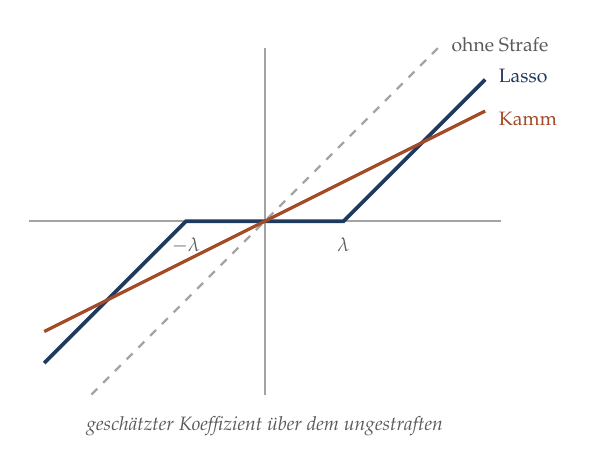
\begin{tikzpicture}[scale=1.0]
\draw[grau!55, line width=0.6pt] (-3,0) -- (3,0);
\draw[grau!55, line width=0.6pt] (0,-2.2) -- (0,2.2);
\draw[grau!55, line width=0.8pt, dashed] (-2.2,-2.2) -- (2.2,2.2);
\draw[tief, line width=1.4pt] (-2.8,-1.8) -- (-1,0) -- (1,0) -- (2.8,1.8);
\draw[akzent, line width=1.2pt] (-2.8,-1.4) -- (2.8,1.4);
\node[font=\scriptsize, color=grau, anchor=north] at (1,-0.08) {$\lambda$};
\node[font=\scriptsize, color=grau, anchor=north] at (-1,-0.08) {$-\lambda$};
\node[font=\scriptsize, color=tief, anchor=west] at (2.85,1.85) {Lasso};
\node[font=\scriptsize, color=akzent, anchor=west] at (2.85,1.3) {Kamm};
\node[font=\scriptsize, color=grau, anchor=west] at (2.25,2.25) {ohne Strafe};
\node[font=\scriptsize\itshape, color=grau] at (0,-2.6) {geschätzter Koeffizient über dem ungestraften};
\end{tikzpicture}
\end{center}

\begin{center}
{\small
\renewcommand{\arraystretch}{1.5}
\begin{tabular}{@{}P{2.2cm}P{6.4cm}@{}}
\toprule
\textbf{Kamm} & teilt jeden Koeffizienten durch $1+\lambda$. Nichts wird null.\\
\textbf{Lasso} & zieht von jedem $\lambda$ ab. Was kleiner ist als $\lambda$, wird \textcolor{akzent}{genau null}.\\
\bottomrule
\end{tabular}}
\end{center}

\begin{center}
\begin{minipage}{0.9\textwidth}
\textbf{Das Lasso wählt Merkmale aus --- es setzt die unwichtigen auf null.}
\end{minipage}
\end{center}

\schritt{Warum Beträge das bewirken}
\begin{center}
\begin{minipage}{0.88\textwidth}
\kursiv{Die Betragsfunktion hat bei null einen Knick. \textbf{Eine Strafe mit Knick hält den Koeffizienten bei null fest}, solange der Nutzen einer Abweichung kleiner ist als die Steigung des Knicks. Das Quadrat hat bei null die Steigung null und kann deshalb nie etwas festhalten --- es drückt nur. Geometrisch: Die Menge $\|\vek\beta\|_{1} \le t$ ist eine Raute mit Ecken auf den Achsen, und dort berührt man sie am häufigsten.}
\end{minipage}
\end{center}
\end{merksatz}

\section{Der Leitfall gerechnet}

\begin{merksatz}
\boxtitel{Dreihundert Wiederholungen}
Die Strafstärke wurde jeweils durch fünffache Kreuzvalidierung gewählt; geprüft wurde an $2000$ neuen Patienten.

\begin{center}
{\small
\renewcommand{\arraystretch}{1.5}
\begin{tabular}{@{}P{3.2cm}P{2.4cm}P{2.4cm}@{}}
\toprule
\textbf{Verfahren} & \textbf{Testfehler} & \textbf{über Rauschen}\\
\midrule
kleinste Quadrate & $2{,}19$ & $1{,}19$\\
Kammregression & $1{,}35$ & $0{,}35$\\
Lasso & $\mathbf{1{,}31}$ & $\mathbf{0{,}31}$\\
\midrule
bestmöglich & $1{,}00$ & $0$\\
\bottomrule
\end{tabular}}
\end{center}

\begin{center}
\begin{minipage}{0.9\textwidth}
\textbf{Beide Strafverfahren verringern den vermeidbaren Fehler auf weniger als ein Drittel.}
\end{minipage}
\end{center}

\begin{center}
\begin{minipage}{0.88\textwidth}
\kursiv{Der Überschuss der kleinsten Quadrate von $1{,}19$ liegt nahe an dem, was Satz 2.2 vorhersagt. \textbf{Das Lasso ist hier geringfügig besser als der Kamm}, weil in Wahrheit nur drei Merkmale wirken --- seine Neigung zu dünn besetzten Lösungen passt zur Aufgabe. Wären alle zwanzig Merkmale ein wenig wichtig, läge der Kamm vorn. Das ist Satz 1.5 in praktischer Gestalt.}
\end{minipage}
\end{center}
\end{merksatz}

\section{Der Bruchfall}

\begin{warnung}
\boxtitelr{Was das Lasso auswählt}
Im Leitfall wählte das Lasso im Mittel $5{,}7$ Merkmale --- davon $1{,}8$ der drei wahren.

\begin{center}
{\small
\renewcommand{\arraystretch}{1.5}
\begin{tabular}{@{}P{3.2cm}P{3.2cm}@{}}
\toprule
\textbf{Merkmal} & \textbf{gewählt in}\\
\midrule
wahres Merkmal 1 & $89\,\%$\\
wahres Merkmal 2 & $42\,\%$\\
wahres Merkmal 3 & $55\,\%$\\
jedes falsche & $22\,\%$\\
\bottomrule
\end{tabular}}
\end{center}

\begin{center}
\begin{minipage}{0.9\textwidth}
\textbf{Ein wahres Merkmal wird in mehr als der Hälfte der Fälle übersehen --- und jedes falsche in jedem fünften Fall aufgenommen.}
\end{minipage}
\end{center}

\schritt{Der Grund}
\begin{center}
\begin{minipage}{0.88\textwidth}
\kursiv{Bei verbundenen Merkmalen kann ein falsches ein wahres vertreten --- es trägt dieselbe Information, weil beide gemeinsam schwanken. \textbf{Das Lasso wählt dann eines davon, mehr oder weniger zufällig}, und in der nächsten Stichprobe ein anderes. Die Vorhersage bleibt gut, die Auswahl nicht.}
\end{minipage}
\end{center}

\schritt{Die Folgerung}
\begin{center}
\begin{minipage}{0.88\textwidth}
\kursiv{\textbf{Die vom Lasso gewählten Merkmale sind keine Ursachen und oft nicht einmal die wichtigsten.} Wer aus der Auswahl schließt, welche Laborwerte die Sepsis \enquote{erklären}, verwechselt Vorhersage mit Erklärung --- die dritte Warnung des Vorworts. Gegen die Instabilität hilft, die Auswahl an vielen Teilstichproben zu wiederholen und nur zu berichten, was fast immer gewählt wird; gegen die Verwechslung hilft nichts als Vorsicht.}
\end{minipage}
\end{center}
\end{warnung}

\begin{warnung}
\boxtitelr{Und ein technischer Vorbehalt}
Beide Strafen hängen von der Einheit der Merkmale ab.

\begin{center}
\begin{minipage}{0.88\textwidth}
\kursiv{Misst man das Kreatinin in $\mu$mol/l statt in mg/dl, so wird sein Koeffizient $88$-mal kleiner --- und damit viel weniger bestraft. \textbf{Man muss die Merkmale vorher auf gleiche Streuung bringen}, sonst entscheidet die Wahl der Einheit, was ausgewählt wird. Und nach Kapitel~3 gehört diese Normierung \kursiv{in} die Kreuzvalidierung, nicht davor.}
\end{minipage}
\end{center}
\end{warnung}

\section{Übungsaufgaben}

\begin{aufgabe}
\boxtitel{Aufgabe 4.1 --- Kammregression mit einem Merkmal}
Ein Merkmal, drei Patienten, ohne Achsenabschnitt: $x = (1,2,3)$, $y = (2,3,5)$. Berechnen Sie den Koeffizienten für $\lambda = 0$, $1$, $7$ und $\infty$.

\loesung
\schritt{Schritt 1 --- Die Formel in einer Dimension}
Satz 4.2 wird zu
\[ \hat\beta_{\lambda} = \frac{\sum x_i y_i}{\sum x_i^{2} + \lambda} . \]

\schritt{Schritt 2 --- Die Summen}
\[ \sum x_i y_i = 1\cdot2 + 2\cdot3 + 3\cdot5 = 2+6+15 = 23 \]
\[ \sum x_i^{2} = 1+4+9 = 14 \]

\schritt{Schritt 3 --- Die Werte}
\begin{center}
{\small
\renewcommand{\arraystretch}{1.48}
\begin{tabular}{@{}P{1.6cm}P{2.4cm}P{2.0cm}P{2.0cm}@{}}
\toprule
$\lambda$ & \textbf{Rechnung} & $\hat\beta$ & \textbf{Faktor}\\
\midrule
$0$ & $23/14$ & $1{,}643$ & $1{,}00$\\
$1$ & $23/15$ & $1{,}533$ & $0{,}93$\\
$7$ & $23/21$ & $1{,}095$ & $0{,}67$\\
$\infty$ & --- & $0$ & $0$\\
\bottomrule
\end{tabular}}
\end{center}

\kursiv{Zur letzten Spalte:} $\frac{14}{14+\lambda}$, also $\frac{d^{2}}{d^{2}+\lambda}$ mit $d^{2} = 14$.

\schritt{Schritt 4 --- Die Probe}
Bei $\lambda = 7$: $1{,}643\cdot\frac{14}{21} = 1{,}643\cdot0{,}667 = 1{,}095$ \checkmark

\begin{center}
\begin{minipage}{0.88\textwidth}
\kursiv{\textbf{Die Strafe wirkt umso schwächer, je mehr Information die Daten haben.} Bei hundert Patienten mit ähnlichen Werten wäre $\sum x_i^{2}$ etwa $470$, und $\lambda = 7$ schrumpfte nur um anderthalb Prozent. Man muss $\lambda$ also mit $n$ zusammen sehen --- was die Kreuzvalidierung von selbst erledigt.}
\end{minipage}
\end{center}
\end{aufgabe}

\begin{aufgabe}
\boxtitel{Aufgabe 4.2 --- Das Lasso von Hand}
Bei orthonormalen Merkmalen liefern kleinste Quadrate die Koeffizienten
\[ \vek b = (0{,}90;\ -0{,}40;\ 0{,}15;\ 0{,}05;\ -0{,}60) . \]
Berechnen Sie Lasso und Kammregression für $\lambda = 0{,}2$ und $\lambda = 0{,}5$.

\loesung
\schritt{Schritt 1 --- Das Lasso nach Satz 4.4}
\begin{center}
{\small
\renewcommand{\arraystretch}{1.48}
\begin{tabular}{@{}P{1.6cm}P{2.2cm}P{2.2cm}@{}}
\toprule
$b_j$ & $\lambda = 0{,}2$ & $\lambda = 0{,}5$\\
\midrule
$0{,}90$ & $0{,}70$ & $0{,}40$\\
$-0{,}40$ & $-0{,}20$ & $\mathbf{0}$\\
$0{,}15$ & $\mathbf{0}$ & $\mathbf{0}$\\
$0{,}05$ & $\mathbf{0}$ & $\mathbf{0}$\\
$-0{,}60$ & $-0{,}40$ & $-0{,}10$\\
\midrule
\textbf{ungleich null} & $3$ & $2$\\
\bottomrule
\end{tabular}}
\end{center}

\kursiv{Beispiel zweite Zeile, $\lambda = 0{,}5$:} $|{-0{,}40}| - 0{,}5 = -0{,}10 < 0$, also null.

\schritt{Schritt 2 --- Die Kammregression}
Bei orthonormalen Merkmalen und der Strafe $\frac{\lambda}{2}\|\vek\beta\|^{2}$ passend zu Definition 4.3 gilt $\hat\beta_j = \frac{b_j}{1+\lambda}$.

\begin{center}
{\small
\renewcommand{\arraystretch}{1.48}
\begin{tabular}{@{}P{1.6cm}P{2.2cm}P{2.2cm}@{}}
\toprule
$b_j$ & $\lambda = 0{,}2$ & $\lambda = 0{,}5$\\
\midrule
$0{,}90$ & $0{,}750$ & $0{,}600$\\
$-0{,}40$ & $-0{,}333$ & $-0{,}267$\\
$0{,}15$ & $0{,}125$ & $0{,}100$\\
$0{,}05$ & $0{,}042$ & $0{,}033$\\
$-0{,}60$ & $-0{,}500$ & $-0{,}400$\\
\bottomrule
\end{tabular}}
\end{center}

\schritt{Schritt 3 --- Der Vergleich}
\begin{center}
\begin{minipage}{0.9\textwidth}
\textbf{Der Kamm schrumpft alle im selben Verhältnis. Das Lasso zieht von allen dasselbe ab --- und die kleinen verschwinden.}
\end{minipage}
\end{center}

\begin{center}
\begin{minipage}{0.88\textwidth}
\kursiv{Das hat eine unerwünschte Nebenwirkung: \textbf{Das Lasso verkleinert auch die großen Koeffizienten um volle $\lambda$} --- der wichtigste wird bei $\lambda = 0{,}5$ von $0{,}90$ auf $0{,}40$ gedrückt, mehr als halbiert. Deshalb passt man in der Praxis oft das Modell nach der Auswahl noch einmal ohne Strafe an, nur mit den gewählten Merkmalen. Das hebt die Verzerrung auf, bringt aber die Varianz teilweise zurück.}
\end{minipage}
\end{center}
\end{aufgabe}

\begin{aufgabe}
\boxtitel{Aufgabe 4.3 --- Zwei fast gleiche Merkmale}
Kreatinin und Harnstoff haben bei den Patienten eine Korrelation von $\rho = 0{,}95$. Beide sind auf Streuung eins gebracht. Die Varianz eines Koeffizienten wäre bei unverbundenen Merkmalen $0{,}05$. Wie groß ist sie hier, und was bewirkt der Kamm?

\loesung
\schritt{Schritt 1 --- Der Varianzfaktor}
\[ \frac{1}{1-\rho^{2}} = \frac{1}{1-0{,}9025} = \frac{1}{0{,}0975} = 10{,}26 \]

\schritt{Schritt 2 --- Die Varianz}
\[ 0{,}05\cdot10{,}26 = 0{,}513 \]
\[ \text{Streuung} = \sqrt{0{,}513} = 0{,}716 \]

\begin{center}
\begin{minipage}{0.9\textwidth}
\textbf{Ein Koeffizient von etwa $0{,}5$ schwankt um $\pm0{,}72$} --- sein Vorzeichen ist praktisch nicht bestimmbar.
\end{minipage}
\end{center}

\schritt{Schritt 3 --- Die beiden Richtungen}
Die Matrix $X^{\!\top}X/n$ der beiden Merkmale ist
\[ \begin{pmatrix} 1 & 0{,}95\\ 0{,}95 & 1\end{pmatrix} \]
mit den Eigenwerten $1+\rho = 1{,}95$ (Summe beider) und $1-\rho = 0{,}05$ (Differenz beider).

\begin{center}
{\small
\renewcommand{\arraystretch}{1.5}
\begin{tabular}{@{}P{2.6cm}P{1.8cm}P{3.2cm}@{}}
\toprule
\textbf{Richtung} & \textbf{Eigenwert} & \textbf{Kammfaktor, $\lambda/n = 0{,}1$}\\
\midrule
Summe & $1{,}95$ & $1{,}95/2{,}05 = 0{,}95$\\
Differenz & $0{,}05$ & $0{,}05/0{,}15 = 0{,}33$\\
\bottomrule
\end{tabular}}
\end{center}

\begin{center}
\begin{minipage}{0.88\textwidth}
\kursiv{\textbf{Der Kamm lässt die gemeinsame Wirkung fast unberührt und dämpft den Unterschied auf ein Drittel.} Das ist genau richtig: Wie stark \enquote{die Nierenwerte} insgesamt wirken, lässt sich gut schätzen; welcher der beiden es ist, kaum. Der Kamm verteilt die Wirkung dann ungefähr gleich auf beide, statt zufällig einem den Löwenanteil zu geben.}
\end{minipage}
\end{center}

\schritt{Schritt 4 --- Und das Lasso?}
\begin{center}
\begin{minipage}{0.88\textwidth}
\kursiv{Es wählt eines der beiden und setzt das andere auf null --- welches, hängt vom Zufall der Stichprobe ab. \textbf{Für die Vorhersage macht das wenig, für die Deutung viel.} Wer beides will, benutzt eine Mischung beider Strafen, das sogenannte elastische Netz, das verbundene Merkmale gemeinsam aufnimmt oder gemeinsam verwirft.}
\end{minipage}
\end{center}
\end{aufgabe}

\begin{geschichte}
\boxtitelg{Tichonow, Hoerl und Tibshirani}
\Person{Andrei Tichonow} (1906--1993) führte die Idee 1943 in der Sowjetunion ein, um schlecht gestellte Probleme der Geophysik zu lösen.

\begin{center}
\begin{minipage}{0.9\textwidth}
\kursiv{Wer aus Messungen an der Erdoberfläche auf Gesteinsschichten schließen will, hat mehr Unbekannte als Messungen. Tichonow fügte eine Strafe für \enquote{unruhige} Lösungen hinzu. \textbf{In der Numerik heißt das Verfahren bis heute Tichonow-Regularisierung} --- es ist dasselbe wie die Kammregression, dreißig Jahre früher und in anderer Sprache.}
\end{minipage}
\end{center}

\schritt{Der Name}
\Person{Arthur Hoerl} und \Person{Robert Kennard} veröffentlichten 1970 die Kammregression für die Statistik.

\begin{center}
\begin{minipage}{0.9\textwidth}
\kursiv{Der Name stammt aus Hoerls früherer Arbeit über Wirkungsflächen in der Chemie, wo er von \enquote{Kammanalyse} sprach --- der Suche nach Graten in einer Fläche. \textbf{Der Zusammenhang mit der heutigen Bedeutung ist eher lose}, der Name hat sich trotzdem gehalten.}
\end{minipage}
\end{center}

\schritt{Das Lasso}
\Person{Robert Tibshirani} veröffentlichte das Lasso 1996.

\begin{center}
\begin{minipage}{0.9\textwidth}
\kursiv{Der Name ist eine Abkürzung, soll aber zugleich an das Lasso des Viehhirten erinnern, das Merkmale einfängt. \textbf{Die Idee war nicht ganz neu} --- Geophysiker hatten die Betragsstrafe schon in den 1970er Jahren verwendet ---, aber Tibshirani gab die statistische Begründung. Der Aufsatz gehört zu den meistzitierten der Statistik überhaupt.}
\end{minipage}
\end{center}
\end{geschichte}

\begin{forschung}
\boxtitelp{Strafen heute}
\begin{center}
{\small
\renewcommand{\arraystretch}{1.45}
\begin{tabular}{@{}P{2.8cm}P{5.4cm}@{}}
\toprule
\textbf{Nach der Auswahl schließen} & Gültige Vertrauensintervalle für Koeffizienten, die das Lasso ausgewählt hat.\\
\textbf{Stabilitäts\-auswahl} & Nur berichten, was über viele Teilstichproben stabil gewählt wird.\\
\textbf{Komprimiertes Messen} & Aus wenigen Messungen ein dünn besetztes Signal rekonstruieren.\\
\bottomrule
\end{tabular}}
\end{center}

\schritt{Zur ersten Zeile}
\begin{center}
\begin{minipage}{0.88\textwidth}
\kursiv{Wählt man Merkmale anhand der Daten aus und rechnet dann mit denselben Daten ein Vertrauensintervall, so ist dieses zu schmal --- dasselbe Leck wie in Kapitel~3. \textbf{Seit etwa 2014 gibt es Verfahren, die das korrigieren}, indem sie die Auswahl in die Rechnung einbeziehen. Die Intervalle werden dabei deutlich breiter, was der ehrlichere Befund ist.}
\end{minipage}
\end{center}

\schritt{Zur dritten Zeile}
\begin{center}
\begin{minipage}{0.88\textwidth}
\kursiv{Die Mathematik des Lassos erlaubt es, ein Bild aus weit weniger Messungen zu rekonstruieren, als es Bildpunkte hat --- sofern es in einer geeigneten Darstellung dünn besetzt ist. \textbf{Magnetresonanztomographen nutzen das seit einigen Jahren}, um Aufnahmezeiten erheblich zu verkürzen. Das ist eine der wenigen Stellen, an denen ein Satz der Lerntheorie unmittelbar in einem Gerät steckt, das Patienten begegnet.}
\end{minipage}
\end{center}
\end{forschung}

\begin{merksatz}
\boxtitel{Was Sie jetzt können}
\begin{center}
\renewcommand{\arraystretch}{1.5}
\begin{tabular}{@{}P{3.0cm}P{5.6cm}@{}}
\toprule
\textbf{Kollinearität} & Varianzfaktor $1/(1-\rho^{2})$\\
\textbf{Satz 4.2} & Kamm: $(X^{\!\top}X+\lambda I)^{-1}X^{\!\top}\vek y$\\
\textbf{Schrumpfen} & Faktor $d_j^{2}/(d_j^{2}+\lambda)$\\
\textbf{Satz 4.4} & Lasso: $\operatorname{sign}(b)(|b|-\lambda)_{+}$\\
\textbf{Der Bruchfall} & ausgewählt heißt nicht ursächlich\\
\bottomrule
\end{tabular}
\end{center}

\begin{center}
\begin{minipage}{0.88\textwidth}
\kursiv{Dieses Kapitel sagte einen Zahlenwert vorher. Das nächste sagt eine Wahrscheinlichkeit vorher --- Sepsis ja oder nein --- und findet, dass dieselben Strafen dort genauso wirken, das Minimieren aber schwieriger wird.}
\end{minipage}
\end{center}
\end{merksatz}

\chapter{Eine Wahrscheinlichkeit vorhersagen}

\section{Der Leitfall}

\begin{merksatz}
\boxtitel{Zwei Merkmale}
Zum Laktat kommt nun die Herzfrequenz. Bei $400$ Patienten der Intensivstation liegen beide Werte vor; $10$ Prozent entwickeln eine Sepsis.

\begin{center}
{\small
\renewcommand{\arraystretch}{1.5}
\begin{tabular}{@{}P{2.4cm}P{2.8cm}P{2.8cm}@{}}
\toprule
& \textbf{ohne Sepsis} & \textbf{mit Sepsis}\\
\midrule
Laktat & um $1{,}2$ mmol/l & um $3{,}0$ mmol/l\\
Herzfrequenz & um $88$/min & um $112$/min\\
\bottomrule
\end{tabular}}
\end{center}

\textbf{Gesucht:} nicht nur ein Ja oder Nein, sondern eine Wahrscheinlichkeit.

\begin{center}
\begin{minipage}{0.88\textwidth}
\kursiv{Eine Wahrscheinlichkeit ist mehr wert als eine Entscheidung. \textbf{Man kann sie nachträglich mit jeder Kostenrechnung aus Kapitel~1 verbinden} --- die Schwelle wird erst gewählt, wenn feststeht, was ein Fehler kostet. Ein Verfahren, das nur Ja oder Nein ausgibt, hat diese Entscheidung bereits getroffen, ohne sie offenzulegen.}
\end{minipage}
\end{center}
\end{merksatz}

\section{Das Modell}

\begin{merksatz}
\boxtitel{Warum nicht einfach eine Gerade?}
Eine lineare Funktion $\beta_0 + \vek\beta^{\!\top}\vek x$ nimmt jeden Wert an --- auch negative und solche über eins. Eine Wahrscheinlichkeit darf das nicht.

\schritt{Der Ausweg: Chancen statt Wahrscheinlichkeiten}
\begin{center}
{\small
\renewcommand{\arraystretch}{1.5}
\begin{tabular}{@{}P{3.0cm}P{2.4cm}P{2.4cm}@{}}
\toprule
\textbf{Größe} & \textbf{Formel} & \textbf{Bereich}\\
\midrule
Wahrscheinlichkeit & $p$ & $0$ bis $1$\\
Chance & $\dfrac{p}{1-p}$ & $0$ bis $\infty$\\
Logarithmus der Chance & $\ln\dfrac{p}{1-p}$ & $-\infty$ bis $\infty$\\
\bottomrule
\end{tabular}}
\end{center}

\begin{center}
\begin{minipage}{0.9\textwidth}
\textbf{Der Logarithmus der Chance nimmt jeden Wert an --- und darf daher linear sein.}
\end{minipage}
\end{center}
\end{merksatz}

\begin{definition}
\boxtitelm{Definition 5.1 --- logistische Regression}
\[ \ln\frac{p(\vek x)}{1-p(\vek x)} = \beta_0 + \vek\beta^{\!\top}\vek x \]
oder gleichwertig
\[ p(\vek x) = \sigma\bigl(\beta_0 + \vek\beta^{\!\top}\vek x\bigr), \qquad \sigma(z) = \frac{1}{1+e^{-z}} . \]
\end{definition}

\begin{merksatz}
\boxtitel{Die Funktion $\sigma$}
\begin{center}
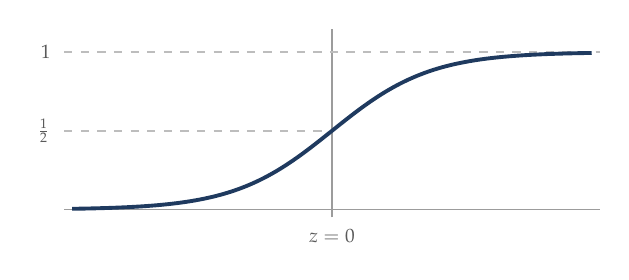
\begin{tikzpicture}[scale=1.0]
\draw[grau!60, line width=0.6pt] (-3.4,0) -- (3.4,0);
\draw[grau!60, line width=0.6pt] (0,-0.1) -- (0,2.3);
\draw[grau!40, line width=0.6pt, dashed] (-3.4,2) -- (3.4,2);
\draw[grau!40, line width=0.6pt, dashed] (-3.4,1) -- (0,1);
\draw[tief, line width=1.4pt, smooth, samples=60, domain=-3.3:3.3] plot ({\x}, {2/(1+exp(-1.6*\x))});
\node[font=\scriptsize, color=grau, anchor=east] at (-3.45,2) {$1$};
\node[font=\scriptsize, color=grau, anchor=east] at (-3.45,1) {$\tfrac12$};
\node[font=\scriptsize, color=grau, anchor=north] at (0,-0.12) {$z = 0$};
\end{tikzpicture}
\end{center}

\begin{center}
{\small
\renewcommand{\arraystretch}{1.5}
\begin{tabular}{@{}P{3.2cm}P{5.4cm}@{}}
\toprule
$\sigma(0) = \tfrac12$ & Bei $z = 0$ ist alles offen.\\
$\sigma(-z) = 1-\sigma(z)$ & Symmetrisch um $\tfrac12$.\\
$\sigma'(z) = \sigma(z)\,(1-\sigma(z))$ & Am steilsten in der Mitte.\\
\bottomrule
\end{tabular}}
\end{center}

\kursiv{Zur dritten Zeile:} $\sigma'(z) = \frac{e^{-z}}{(1+e^{-z})^{2}} = \frac{1}{1+e^{-z}}\cdot\frac{e^{-z}}{1+e^{-z}} = \sigma(z)\,(1-\sigma(z))$.

\schritt{Die Deutung der Koeffizienten}
Steigt $x_j$ um eine Einheit, so steigt der Logarithmus der Chance um $\beta_j$ --- die Chance selbst wird mit $e^{\beta_j}$ multipliziert.

\begin{center}
\begin{minipage}{0.9\textwidth}
\textbf{$e^{\beta_j}$ ist das Chancenverhältnis je Einheit von $x_j$} --- die Größe, die in klinischen Studien als \enquote{Odds Ratio} berichtet wird.
\end{minipage}
\end{center}
\end{merksatz}

\section{Was man minimiert}

\begin{merksatz}
\boxtitel{Der Verlust}
Für einen Patienten mit vorhergesagter Wahrscheinlichkeit $p$ und tatsächlichem Ausgang $y \in \{0,1\}$:
\[ \ell(p,y) = -y\,\ln p - (1-y)\,\ln(1-p) \]

\begin{center}
{\small
\renewcommand{\arraystretch}{1.5}
\begin{tabular}{@{}P{2.4cm}P{2.4cm}P{3.0cm}@{}}
\toprule
\textbf{Ausgang} & \textbf{Vorhersage} & \textbf{Verlust}\\
\midrule
Sepsis & $p = 0{,}9$ & $-\ln0{,}9 = 0{,}105$\\
Sepsis & $p = 0{,}5$ & $-\ln0{,}5 = 0{,}693$\\
Sepsis & $p = 0{,}01$ & $-\ln0{,}01 = 4{,}605$\\
\bottomrule
\end{tabular}}
\end{center}

\begin{center}
\begin{minipage}{0.9\textwidth}
\textbf{Wer sich sicher irrt, wird schwer bestraft.}
\end{minipage}
\end{center}

\schritt{Woher der Verlust kommt}
\begin{center}
{\small
\renewcommand{\arraystretch}{1.5}
\begin{tabular}{@{}P{2.4cm}P{6.2cm}@{}}
\toprule
\textbf{Band 17} & Er ist der negative Logarithmus der Likelihood --- Minimieren heißt Maximum-Likelihood-Schätzen.\\
\textbf{Band 20} & Er ist die Kreuzentropie zwischen beobachteter und vorhergesagter Verteilung --- Minimieren heißt, die Kullback-Leibler-Divergenz zu verkleinern.\\
\bottomrule
\end{tabular}}
\end{center}

\begin{center}
\begin{minipage}{0.88\textwidth}
\kursiv{\textbf{Zwei Vorgängerbände, dieselbe Größe.} Der mittlere Verlust ist die Zahl der Bits (mal $\ln 2$), die man bräuchte, um die tatsächlichen Ausgänge zu übermitteln, wenn man das Modell als Codebuch benutzt. Ein gutes Modell ist eines, das die Wirklichkeit kurz beschreibt --- Band 20, Kapitel~8.}
\end{minipage}
\end{center}
\end{merksatz}

\begin{merksatz}
\boxtitel{Satz 5.2 --- Gradient und Konvexität}
Mit $p_i = \sigma(\vek\beta^{\!\top}\vek x_i)$ --- den Achsenabschnitt als Merkmal $x_{i0} = 1$ eingerechnet --- gilt für den Gesamtverlust $J(\vek\beta) = \sum_i \ell(p_i,y_i)$:
\[ \nabla J(\vek\beta) = \sum_i (p_i - y_i)\,\vek x_i , \qquad \nabla^{2}J(\vek\beta) = \sum_i p_i(1-p_i)\,\vek x_i\vek x_i^{\!\top} . \]
Insbesondere ist $J$ konvex.

\schritt{Beweis}
\kursiv{Die Ableitung nach $z$:} Mit $\sigma' = \sigma(1-\sigma)$ ist
\[ \frac{\dd}{\dd z}\bigl[-y\ln\sigma(z)\bigr] = -y\,(1-\sigma), \qquad \frac{\dd}{\dd z}\bigl[-(1-y)\ln(1-\sigma(z))\bigr] = (1-y)\,\sigma . \]
Summe: $-y + y\sigma + \sigma - y\sigma = \sigma - y$.

\kursiv{Nach der Kettenregel} mit $z = \vek\beta^{\!\top}\vek x$ kommt der Faktor $\vek x$ hinzu. Das ist der Gradient.

\kursiv{Nochmals ableiten:} $\frac{\dd}{\dd z}(\sigma - y) = \sigma(1-\sigma)$, mal $\vek x\vek x^{\!\top}$.

\kursiv{Konvexität:} Für jeden Vektor $\vek v$ ist
\[ \vek v^{\!\top}\nabla^{2}J\,\vek v = \sum_i p_i(1-p_i)\,(\vek x_i^{\!\top}\vek v)^{2} \ \ge\ 0 , \]
denn alle Summanden sind nichtnegativ. Nach Band 19, Kapitel~7 ist $J$ konvex. $\blacksquare$

\begin{center}
\begin{minipage}{0.9\textwidth}
\textbf{Der Gradient ist die Summe der Vorhersagefehler, gewichtet mit den Merkmalen} --- dieselbe Gestalt wie bei kleinsten Quadraten.
\end{minipage}
\end{center}

\begin{center}
\begin{minipage}{0.88\textwidth}
\kursiv{\textbf{Konvexität bedeutet: Jedes lokale Minimum ist ein globales} (Band 19, Satz 7.3). Man kann nicht in einer Mulde steckenbleiben. Das ist keine Selbstverständlichkeit --- bei den Netzen aus Kapitel~11 geht genau diese Eigenschaft verloren.}
\end{minipage}
\end{center}
\end{merksatz}

\section{Wie man minimiert}

\begin{merksatz}
\boxtitel{Keine geschlossene Lösung}
Anders als bei kleinsten Quadraten lässt sich $\nabla J = \vek 0$ nicht nach $\vek\beta$ auflösen --- $\vek\beta$ steckt in den $p_i$ im Exponenten.

\schritt{Gradientenabstieg}
\[ \vek\beta \ \leftarrow\ \vek\beta - \eta\,\nabla J(\vek\beta) \]
mit einer Schrittweite $\eta > 0$ (Band 19, Kapitel~8).

\schritt{Newton-Verfahren}
\[ \vek\beta \ \leftarrow\ \vek\beta - \bigl(\nabla^{2}J\bigr)^{-1}\nabla J \]

\begin{center}
{\small
\renewcommand{\arraystretch}{1.5}
\begin{tabular}{@{}P{2.4cm}P{3.0cm}P{3.0cm}@{}}
\toprule
& \textbf{Gradient} & \textbf{Newton}\\
\midrule
je Schritt & billig & teuer: Matrix lösen\\
Schritte & viele & wenige\\
bei großem $p$ & geeignet & ungeeignet\\
\bottomrule
\end{tabular}}
\end{center}

\begin{center}
\begin{minipage}{0.88\textwidth}
\kursiv{Das Newton-Verfahren für die logistische Regression hat einen eigenen Namen --- \enquote{iterativ neu gewichtete kleinste Quadrate} ---, weil jeder Schritt eine gewichtete Regression mit den Gewichten $p_i(1-p_i)$ ist. \textbf{Statistikprogramme benutzen es seit Jahrzehnten}; bei Millionen von Merkmalen greift man zum Gradienten.}
\end{minipage}
\end{center}
\end{merksatz}

\section{Der Leitfall gerechnet}

\begin{merksatz}
\boxtitel{Das angepasste Modell}
\[ \ln\frac{p}{1-p} = -20{,}1 + 3{,}33\cdot\text{Laktat} + 0{,}120\cdot\text{Herzfrequenz} \]

\begin{center}
{\small
\renewcommand{\arraystretch}{1.5}
\begin{tabular}{@{}P{3.2cm}P{2.4cm}P{2.4cm}@{}}
\toprule
\textbf{Merkmal} & \textbf{Koeffizient} & \textbf{Chancenverh.}\\
\midrule
Laktat, je mmol/l & $3{,}33$ & $28$\\
Herzfrequenz, je $10$/min & $1{,}20$ & $3{,}3$\\
\bottomrule
\end{tabular}}
\end{center}

\schritt{Geprüft an $20\,000$ neuen Patienten}
\begin{center}
{\small
\renewcommand{\arraystretch}{1.5}
\begin{tabular}{@{}P{3.2cm}P{2.4cm}@{}}
\toprule
\textbf{Merkmale} & \textbf{Trennschärfe}\\
\midrule
nur Herzfrequenz & $0{,}892$\\
nur Laktat & $0{,}944$\\
beide & $\mathbf{0{,}979}$\\
\bottomrule
\end{tabular}}
\end{center}

\begin{center}
\begin{minipage}{0.9\textwidth}
\textbf{Mit zwei Merkmalen sinkt die Fehlerrate auf $2{,}4$ Prozent --- unter das Bayes-Risiko von $3{,}5$ Prozent aus Kapitel~1.}
\end{minipage}
\end{center}

\begin{center}
\begin{minipage}{0.88\textwidth}
\kursiv{Das ist kein Widerspruch: Das Bayes-Risiko galt für \kursiv{nur} das Laktat. \textbf{Mit einem zweiten Merkmal gibt es eine neue, niedrigere Grenze} --- genau die Aussage aus Kapitel~1, dass mehr Merkmale helfen, ein besseres Verfahren nicht. Die Zahlen sind allerdings mit Vorsicht zu lesen; der Bruchfall sagt, warum.}
\end{minipage}
\end{center}
\end{merksatz}

\section{Das Perzeptron}

\begin{merksatz}
\boxtitel{Der Vorläufer}
Man lässt die Wahrscheinlichkeit weg und will nur richtig einordnen. Etiketten $t_i \in \{-1,+1\}$.

\schritt{Das Verfahren von Rosenblatt}
\begin{center}
{\small
\renewcommand{\arraystretch}{1.5}
\begin{tabular}{@{}P{1.0cm}P{7.4cm}@{}}
\toprule
$1$ & Beginne mit $\vek w = \vek 0$.\\
$2$ & Nimm den nächsten Punkt. Ist $t_i\,\vek w^{\!\top}\vek x_i \le 0$ --- falsch eingeordnet ---, setze $\vek w \leftarrow \vek w + t_i\,\vek x_i$.\\
$3$ & Wiederhole, bis alle richtig liegen.\\
\bottomrule
\end{tabular}}
\end{center}

\begin{center}
\begin{minipage}{0.88\textwidth}
\kursiv{Die Korrektur schiebt $\vek w$ in Richtung des falsch eingeordneten Punktes --- oder davon weg, je nach Etikett. \textbf{Es ist ein Gradientenabstieg}, auf einen Verlust angewandt, der nur bei Fehlern etwas kostet.}
\end{minipage}
\end{center}
\end{merksatz}

\begin{merksatz}
\boxtitel{Satz 5.3 --- Novikoff, 1962}
Es gebe einen Einheitsvektor $\vek w^{*}$ und ein $\gamma > 0$ mit $t_i\,\vek w^{*\top}\vek x_i \ge \gamma$ für alle $i$ --- die Daten sind mit Abstand $\gamma$ trennbar. Ferner sei $\|\vek x_i\| \le R$. Dann macht das Perzeptron höchstens
\[ \left(\frac{R}{\gamma}\right)^{2} \]
Korrekturen.

\schritt{Beweis}
Sei $\vek w_k$ der Vektor nach $k$ Korrekturen.

\kursiv{Erstens --- $\vek w_k$ wächst in Richtung $\vek w^{*}$:} Jede Korrektur fügt $t_i\vek x_i$ hinzu, und $t_i\,\vek w^{*\top}\vek x_i \ge \gamma$. Also
\[ \vek w_k^{\!\top}\vek w^{*} \ \ge\ k\,\gamma . \]

\kursiv{Zweitens --- $\vek w_k$ wächst insgesamt langsam:}
\[ \|\vek w_{k}\|^{2} = \|\vek w_{k-1}\|^{2} + 2\,t_i\,\vek w_{k-1}^{\!\top}\vek x_i + \|\vek x_i\|^{2} \ \le\ \|\vek w_{k-1}\|^{2} + R^{2} , \]
denn korrigiert wird nur, wenn $t_i\,\vek w_{k-1}^{\!\top}\vek x_i \le 0$. Also $\|\vek w_k\|^{2} \le k\,R^{2}$.

\kursiv{Drittens --- zusammen:} Nach der Ungleichung von Cauchy-Schwarz mit $\|\vek w^{*}\| = 1$:
\[ k\,\gamma \ \le\ \vek w_k^{\!\top}\vek w^{*} \ \le\ \|\vek w_k\| \ \le\ \sqrt k\,R \]
\[ \Longrightarrow\quad \sqrt k \ \le\ \frac{R}{\gamma} \quad\Longrightarrow\quad k \ \le\ \left(\frac{R}{\gamma}\right)^{2} \]
$\blacksquare$

\begin{center}
\begin{minipage}{0.9\textwidth}
\textbf{Die Zahl der Fehler hängt nicht von der Zahl der Punkte ab, nicht von der Dimension --- nur vom Verhältnis zwischen Größe der Daten und Breite der Lücke.}
\end{minipage}
\end{center}

\begin{center}
\begin{minipage}{0.88\textwidth}
\kursiv{\textbf{Das ist der erste Satz des Faches, der eine Aussage über Lernen ohne Bezug auf die Dimension macht.} Er kündigt an, was Kapitel~6 und 7 ausbauen: Nicht die Zahl der Parameter entscheidet, sondern eine geometrische Größe --- hier der Abstand $\gamma$, später der Rand der Stützvektormaschine.}
\end{minipage}
\end{center}
\end{merksatz}

\section{Der Bruchfall}

\begin{warnung}
\boxtitelr{Wenn die Daten zu gut sind}
Lassen sich die beiden Gruppen vollständig durch eine Gerade trennen, so hat die logistische Regression \textcolor{akzent}{kein Minimum}.

\schritt{Warum}
\begin{center}
\begin{minipage}{0.88\textwidth}
\kursiv{Liegt jeder Sepsispatient auf der einen Seite, so kann man $\vek\beta$ beliebig vergrößern: Alle $p_i$ rücken näher an null oder eins, und der Verlust sinkt immer weiter gegen null, ohne ihn je zu erreichen. \textbf{Das Verfahren läuft ins Unendliche}, die Koeffizienten werden riesig, und die Programme melden entweder einen Fehler oder liefern unsinnige Zahlen ohne Warnung.}
\end{minipage}
\end{center}

\schritt{Wann das vorkommt}
\begin{center}
{\small
\renewcommand{\arraystretch}{1.5}
\begin{tabular}{@{}P{2.4cm}P{6.2cm}@{}}
\toprule
\textbf{Wenig Fälle} & Bei seltenen Ausgängen und kleinen Stichproben häufig.\\
\textbf{Viele Merkmale} & Bei $p \ge n$ fast immer --- es gibt dann stets eine trennende Ebene.\\
\textbf{Ein Leck} & Ein Merkmal aus der Zukunft (Kapitel~3) trennt oft perfekt.\\
\bottomrule
\end{tabular}}
\end{center}

\schritt{Die Abhilfe}
\begin{center}
\begin{minipage}{0.88\textwidth}
\kursiv{Eine Strafe aus Kapitel~4 --- $\lambda\|\vek\beta\|^{2}$ --- verhindert das Davonlaufen, weil große Koeffizienten nun etwas kosten. \textbf{Die Strafe ist hier nicht Verfeinerung, sondern Voraussetzung dafür, dass es überhaupt eine Lösung gibt.} Eine perfekte Trennung in den Trainingsdaten ist zudem ein Alarmzeichen: Entweder ist das Problem trivial, oder es gibt ein Leck.}
\end{minipage}
\end{center}
\end{warnung}

\begin{warnung}
\boxtitelr{Warum der Leitfall zu gut ist}
\begin{center}
\begin{minipage}{0.88\textwidth}
\kursiv{Die Trennschärfe von $0{,}979$ stammt aus erzeugten Daten mit zwei sauber getrennten Normalverteilungen. \textbf{Echte Sepsismodelle erreichen $0{,}75$ bis $0{,}85$} --- intern. Die Nachprüfung von 2021 ergab $0{,}63$. Der Abstand zwischen Lehrbuchbeispiel und Klinik ist also erheblich, und er entsteht aus allem, was die Simulation weglässt: fehlende Werte, Messzeitpunkte, uneinheitliche Etiketten, andere Patienten.}
\end{minipage}
\end{center}
\end{warnung}

\section{Übungsaufgaben}

\begin{aufgabe}
\boxtitel{Aufgabe 5.1 --- Ein Modell lesen}
Ein Modell lautet
\[ \ln\frac{p}{1-p} = -6 + 1{,}5\cdot\text{Laktat} + 0{,}03\cdot\text{Herzfrequenz} . \]
Berechnen Sie die Sepsiswahrscheinlichkeit für vier Patienten und deuten Sie die Koeffizienten.

\loesung
\schritt{Schritt 1 --- Die Patienten}
\begin{center}
{\small
\renewcommand{\arraystretch}{1.48}
\begin{tabular}{@{}P{1.4cm}P{1.2cm}P{3.0cm}P{1.2cm}P{1.2cm}@{}}
\toprule
\textbf{Laktat} & \textbf{HF} & $z$ & $p$ & \\
\midrule
$1{,}2$ & $85$ & $-6+1{,}8+2{,}55 = -1{,}65$ & $0{,}161$ & \\
$2{,}0$ & $100$ & $-6+3{,}0+3{,}00 = 0$ & $0{,}500$ & \\
$3{,}0$ & $110$ & $-6+4{,}5+3{,}30 = 1{,}80$ & $0{,}858$ & \\
$4{,}0$ & $120$ & $-6+6{,}0+3{,}60 = 3{,}60$ & $0{,}973$ & \\
\bottomrule
\end{tabular}}
\end{center}

\kursiv{Beispiel dritte Zeile:} $p = \frac{1}{1+e^{-1{,}8}} = \frac{1}{1+0{,}165} = 0{,}858$.

\schritt{Schritt 2 --- Die Chancenverhältnisse}
\[ e^{1{,}5} = 4{,}48 \quad\text{je mmol/l Laktat} \]
\[ e^{0{,}03\cdot10} = e^{0{,}3} = 1{,}35 \quad\text{je $10$/min Herzfrequenz} \]

\schritt{Schritt 3 --- Eine häufige Fehldeutung}
\begin{center}
\begin{minipage}{0.9\textwidth}
\textbf{\enquote{Ein mmol/l mehr Laktat macht die Sepsis $4{,}5$-mal so wahrscheinlich} --- das ist falsch.}
\end{minipage}
\end{center}

\kursiv{Die Chance vervierfacht sich, nicht die Wahrscheinlichkeit.} Von Laktat $2{,}0$ auf $3{,}0$ bei gleicher Herzfrequenz $100$:
\[ z: 0 \to 1{,}5, \qquad p: 0{,}500 \to 0{,}818 \]
Die Wahrscheinlichkeit steigt um den Faktor $1{,}64$, die Chance von $1$ auf $4{,}48$.

\begin{center}
\begin{minipage}{0.88\textwidth}
\kursiv{Bei seltenen Ereignissen, wo $p$ klein ist, sind Chance und Wahrscheinlichkeit fast gleich --- dort stimmt die Fehldeutung näherungsweise. \textbf{Bei häufigen Ereignissen überschätzt sie den Effekt erheblich}, und in klinischen Veröffentlichungen geschieht das regelmäßig.}
\end{minipage}
\end{center}
\end{aufgabe}

\begin{aufgabe}
\boxtitel{Aufgabe 5.2 --- Gradientenabstieg von Hand}
Vier Patienten, ein Merkmal, kein Achsenabschnitt: $x = (-1, 0, 1, 2)$, $y = (0, 1, 0, 1)$. Führen Sie zwei Schritte mit $\eta = 0{,}5$ aus, beginnend bei $\beta = 0$.

\loesung
\schritt{Schritt 1 --- Bei $\beta = 0$}
Alle $p_i = \sigma(0) = 0{,}5$.

\[ \nabla J = \sum_i (p_i-y_i)\,x_i = (0{,}5)(-1) + (-0{,}5)(0) + (0{,}5)(1) + (-0{,}5)(2) \]
\[ = -0{,}5 + 0 + 0{,}5 - 1{,}0 = -1{,}0 \]

\[ J(0) = 4\cdot(-\ln0{,}5) = 4\cdot0{,}693 = 2{,}773 \]

\schritt{Schritt 2 --- Der erste Schritt}
\[ \beta = 0 - 0{,}5\cdot(-1{,}0) = 0{,}5 \]

\schritt{Schritt 3 --- Bei $\beta = 0{,}5$}
\begin{center}
{\small
\renewcommand{\arraystretch}{1.46}
\begin{tabular}{@{}P{1.0cm}P{1.0cm}P{1.8cm}P{2.0cm}P{2.0cm}@{}}
\toprule
$x$ & $y$ & $p = \sigma(0{,}5x)$ & $(p-y)\,x$ & $\ell$\\
\midrule
$-1$ & $0$ & $0{,}378$ & $-0{,}378$ & $0{,}474$\\
$0$ & $1$ & $0{,}500$ & $0$ & $0{,}693$\\
$1$ & $0$ & $0{,}622$ & $0{,}622$ & $0{,}974$\\
$2$ & $1$ & $0{,}731$ & $-0{,}538$ & $0{,}313$\\
\midrule
& & & $\mathbf{-0{,}293}$ & $\mathbf{2{,}455}$\\
\bottomrule
\end{tabular}}
\end{center}

\schritt{Schritt 4 --- Der zweite Schritt}
\[ \beta = 0{,}5 - 0{,}5\cdot(-0{,}293) = 0{,}5+0{,}147 = 0{,}647 \]

\schritt{Schritt 5 --- Der weitere Verlauf}
\begin{center}
{\small
\renewcommand{\arraystretch}{1.46}
\begin{tabular}{@{}P{1.6cm}P{1.8cm}P{1.8cm}P{2.0cm}@{}}
\toprule
\textbf{Schritt} & $\beta$ & $J$ & \textbf{Gradient}\\
\midrule
$0$ & $0{,}000$ & $2{,}773$ & $-1{,}000$\\
$1$ & $0{,}500$ & $2{,}455$ & $-0{,}293$\\
$2$ & $0{,}647$ & $2{,}425$ & $-0{,}118$\\
$3$ & $0{,}706$ & $2{,}420$ & $-0{,}053$\\
$5$ & $0{,}745$ & $2{,}418$ & $-0{,}012$\\
\midrule
Minimum & $0{,}756$ & $2{,}418$ & $0$\\
\bottomrule
\end{tabular}}
\end{center}

\begin{center}
\begin{minipage}{0.88\textwidth}
\kursiv{\textbf{Der Gradient halbiert sich etwa mit jedem Schritt} --- lineare Konvergenz im Sinne von Band 19, Kapitel~8. Die Daten sind nicht trennbar (der Patient bei $x = 0$ hat Sepsis, der bei $x = 1$ nicht), deshalb gibt es ein endliches Minimum. Mit $y = (0,0,1,1)$ wären sie trennbar, und $\beta$ würde ohne Ende wachsen.}
\end{minipage}
\end{center}
\end{aufgabe}

\begin{aufgabe}
\boxtitel{Aufgabe 5.3 --- Das Perzeptron von Hand}
Vier Patienten mit Laktatwerten $1{,}0$ ($-$), $3{,}0$ ($+$), $1{,}5$ ($-$), $2{,}5$ ($+$). Mit dem Achsenabschnitt wird $\vek x = (1, \text{Laktat})$. Führen Sie das Perzeptron aus und vergleichen Sie mit Satz 5.3.

\loesung
\schritt{Schritt 1 --- Der Verlauf}
\begin{center}
{\small
\renewcommand{\arraystretch}{1.46}
\begin{tabular}{@{}P{1.4cm}P{1.0cm}P{1.8cm}P{1.6cm}P{2.0cm}@{}}
\toprule
\textbf{Laktat} & $t$ & $\vek w^{\!\top}\vek x$ & \textbf{falsch?} & \textbf{neues} $\vek w$\\
\midrule
$1{,}0$ & $-1$ & $0$ & ja & $(-1;\ -1)$\\
$3{,}0$ & $+1$ & $-4$ & ja & $(0;\ 2)$\\
$1{,}5$ & $-1$ & $3$ & ja & $(-1;\ 0{,}5)$\\
$2{,}5$ & $+1$ & $0{,}25$ & nein & \\
\midrule
$1{,}0$ & $-1$ & $-0{,}5$ & nein & \\
$3{,}0$ & $+1$ & $0{,}5$ & nein & \\
$1{,}5$ & $-1$ & $-0{,}25$ & nein & \\
$2{,}5$ & $+1$ & $0{,}25$ & nein & \\
\bottomrule
\end{tabular}}
\end{center}

\kursiv{Zur ersten Korrektur:} $\vek w = \vek 0 + (-1)\cdot(1;\ 1{,}0) = (-1;\ -1)$.\\
\kursiv{Zur zweiten:} $\vek w = (-1;\ -1) + (+1)\cdot(1;\ 3{,}0) = (0;\ 2)$.\\
\kursiv{Zur dritten:} $\vek w = (0;\ 2) + (-1)\cdot(1;\ 1{,}5) = (-1;\ 0{,}5)$.

\begin{center}
\begin{minipage}{0.9\textwidth}
\textbf{Drei Korrekturen. Die Grenze liegt bei $-1 + 0{,}5\cdot\text{Laktat} = 0$, also Laktat $= 2{,}0$.}
\end{minipage}
\end{center}

\schritt{Schritt 2 --- Die Schranke}
\kursiv{$R$:} Der größte Punkt ist $(1;\ 3)$ mit Länge $\sqrt{10} = 3{,}162$.

\kursiv{$\gamma$:} Die beste Trennung liegt bei Laktat $2$, also $\vek w^{*} = \frac{(-2;\ 1)}{\sqrt5}$. Der kleinste Abstand betrifft die Punkte bei $1{,}5$ und $2{,}5$:
\[ \gamma = \frac{0{,}5}{\sqrt5} = \frac{0{,}5}{2{,}236} = 0{,}224 \]

\[ \left(\frac{R}{\gamma}\right)^{2} = \frac{10}{0{,}05} = 200 \]

\begin{center}
\begin{minipage}{0.9\textwidth}
\textbf{Die Schranke erlaubt zweihundert Korrekturen --- gebraucht wurden drei.}
\end{minipage}
\end{center}

\schritt{Schritt 3 --- Was das über den Satz sagt}
\begin{center}
\begin{minipage}{0.88\textwidth}
\kursiv{Die Schranke gilt für die \kursiv{ungünstigste} Reihenfolge der Punkte und ist entsprechend pessimistisch. \textbf{Worst-Case-Schranken sind in der Lerntheorie die Regel und meist weit von dem entfernt, was man beobachtet} --- ein Muster, das in Kapitel~7 und 8 wiederkehrt. Ihr Wert liegt nicht in der Zahl, sondern in der Form: Sie zeigt, wovon die Schwierigkeit abhängt.}
\end{minipage}
\end{center}

\schritt{Schritt 4 --- Und wenn der Achsenabschnitt fehlte?}
\begin{center}
\begin{minipage}{0.88\textwidth}
\kursiv{Ohne die $1$ in $\vek x$ müsste die Grenze durch den Nullpunkt gehen --- bei Laktat $0$. \textbf{Dann gäbe es keine Trennung}, weil alle Werte positiv sind, und das Perzeptron liefe ohne Ende. Der Achsenabschnitt ist also kein technisches Beiwerk, sondern die Möglichkeit, die Schwelle zu verschieben.}
\end{minipage}
\end{center}
\end{aufgabe}

\begin{geschichte}
\boxtitelg{Eine Maschine, ein Buch und ein Winter}
\Person{Frank Rosenblatt} (1928--1971), Psychologe an der Cornell University, stellte das Perzeptron 1958 vor --- als Modell des Lernens im Gehirn.

\begin{center}
\begin{minipage}{0.9\textwidth}
\kursiv{Er baute es als Maschine mit $400$ Lichtsensoren, deren Gewichte über Motoren an Potentiometern verstellt wurden. \textbf{Die \kursiv{New York Times} berichtete, die Marine erwarte eine Maschine, die gehen, sprechen, sehen, schreiben und sich ihrer selbst bewusst sein werde.} Rosenblatt selbst war vorsichtiger, aber nicht sehr.}
\end{minipage}
\end{center}

\schritt{Das Buch}
\Person{Marvin Minsky} und \Person{Seymour Papert} veröffentlichten 1969 das Buch \kursiv{Perceptrons}.

\begin{center}
\begin{minipage}{0.9\textwidth}
\kursiv{Sie zeigten genau, was ein einzelnes Perzeptron nicht kann --- etwa entscheiden, ob zwei Merkmale \kursiv{verschieden} sind, die sogenannte XOR-Aufgabe. \textbf{Das Buch wurde weithin als Nachweis gelesen, dass neuronale Netze überhaupt nichts taugen}, obwohl es sich auf eine Schicht beschränkte. Die Forschungsmittel versiegten für fast zwei Jahrzehnte.}
\end{minipage}
\end{center}

\schritt{Rosenblatts Ende}
\begin{center}
\begin{minipage}{0.9\textwidth}
\kursiv{Rosenblatt starb 1971 bei einem Bootsunfall an seinem dreiundvierzigsten Geburtstag. \textbf{Er erlebte weder die Rückkehr der Netze in den 1980er Jahren noch ihren Siegeszug nach 2012}; Kapitel~11 erzählt diese Fortsetzung.}
\end{minipage}
\end{center}

\schritt{Die logistische Funktion}
\begin{center}
\begin{minipage}{0.9\textwidth}
\kursiv{Sie stammt von \Person{Pierre-François Verhulst}, der sie 1838 für das Bevölkerungswachstum vorschlug --- dieselbe Kurve, die in Band 18, Kapitel~2 das logistische Wachstum beschreibt. \textbf{Die logistische Regression hat mit Logistik im Sinne von Transport nichts zu tun}; der Name kommt über Verhulsts Kurve vom griechischen Wort für Rechnen.}
\end{minipage}
\end{center}
\end{geschichte}

\begin{forschung}
\boxtitelp{Klassifikation heute}
\begin{center}
{\small
\renewcommand{\arraystretch}{1.45}
\begin{tabular}{@{}P{2.8cm}P{5.4cm}@{}}
\toprule
\textbf{Die Standardfrage} & Sind lernende Verfahren besser als logistische Regression?\\
\textbf{Kalibrierung} & Stimmen die Wahrscheinlichkeiten auch?\\
\textbf{Implizite Neigung} & Wohin läuft der Gradientenabstieg bei trennbaren Daten?\\
\bottomrule
\end{tabular}}
\end{center}

\schritt{Zur ersten Zeile}
\begin{center}
\begin{minipage}{0.88\textwidth}
\kursiv{Eine Übersicht aus dem Jahr 2019 verglich $71$ Studien, die klinische Vorhersagemodelle mit logistischer Regression gegen lernende Verfahren antreten ließen. \textbf{Bei fairer Durchführung fand sie keinen Vorteil der lernenden Verfahren.} Wo sie besser abschnitten, war die logistische Regression meist schlecht angepasst. Bei tabellarischen klinischen Daten mit wenigen Merkmalen ist das einfache Verfahren oft schwer zu schlagen.}
\end{minipage}
\end{center}

\schritt{Zur dritten Zeile}
\begin{center}
\begin{minipage}{0.88\textwidth}
\kursiv{Bei trennbaren Daten läuft $\|\vek\beta\|$ ins Unendliche --- aber seine \kursiv{Richtung} konvergiert. \textbf{Sie konvergiert gegen die Trennung mit dem größten Rand}, wie 2018 gezeigt wurde. Der Gradientenabstieg hat also eine eingebaute Vorliebe, ohne dass man eine Strafe hinzufügt. Das nächste Kapitel macht diese Trennung zum ausdrücklichen Ziel.}
\end{minipage}
\end{center}
\end{forschung}

\begin{merksatz}
\boxtitel{Was Sie jetzt können}
\begin{center}
\renewcommand{\arraystretch}{1.5}
\begin{tabular}{@{}P{3.0cm}P{5.6cm}@{}}
\toprule
\textbf{Definition 5.1} & Logarithmus der Chance ist linear\\
\textbf{Der Verlust} & Kreuzentropie $=$ negative Log-Likelihood\\
\textbf{Satz 5.2} & Gradient $\sum(p_i-y_i)\vek x_i$, konvex\\
\textbf{Satz 5.3} & Perzeptron: höchstens $(R/\gamma)^{2}$ Fehler\\
\textbf{Der Bruchfall} & trennbar heißt: kein Minimum\\
\bottomrule
\end{tabular}
\end{center}

\begin{center}
\begin{minipage}{0.88\textwidth}
\kursiv{Das Perzeptron findet \kursiv{irgendeine} Trennung. Das nächste Kapitel sucht die \kursiv{beste} --- die mit dem breitesten Abstand --- und findet dabei einen Weg, lineare Verfahren auf krumme Grenzen anzuwenden.}
\end{minipage}
\end{center}
\end{merksatz}

\chapter{Der breiteste Streifen}

\section{Der Leitfall}

\begin{merksatz}
\boxtitel{Fieber --- oder Untertemperatur}
Eine Sepsis kann mit Fieber einhergehen, aber auch mit einer Temperatur unter $36$ Grad. Die klassischen Sepsiskriterien tragen dem Rechnung: \enquote{Temperatur über $38$ \kursiv{oder} unter $36$ Grad}.

\begin{center}
{\small
\renewcommand{\arraystretch}{1.5}
\begin{tabular}{@{}P{3.0cm}P{2.6cm}P{2.6cm}@{}}
\toprule
\textbf{Gruppe} & \textbf{Temperatur} & \textbf{Herzfrequenz}\\
\midrule
ohne Sepsis ($80\,\%$) & um $37{,}0$ & um $88$/min\\
Sepsis mit Fieber & um $38{,}9$ & um $108$/min\\
Sepsis unterkühlt & um $35{,}6$ & um $108$/min\\
\bottomrule
\end{tabular}}
\end{center}

\begin{center}
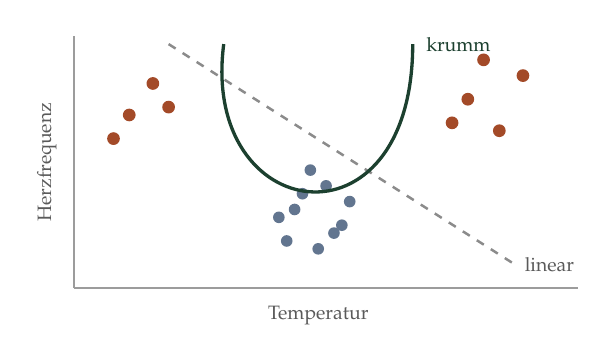
\begin{tikzpicture}[scale=1.0]
\draw[grau!60, line width=0.6pt] (0,0) -- (6.4,0);
\draw[grau!60, line width=0.6pt] (0,0) -- (0,3.2);
\foreach \x/\y in {2.6/0.9,2.9/1.2,3.3/0.7,3.0/1.5,2.7/0.6,3.5/1.1,3.2/1.3,2.8/1.0,3.4/0.8,3.1/0.5}
  \fill[tief!70] (\x,\y) circle (2.1pt);
\foreach \x/\y in {0.7/2.2,1.0/2.6,0.5/1.9,1.2/2.3}
  \fill[akzent] (\x,\y) circle (2.3pt);
\foreach \x/\y in {5.0/2.4,5.4/2.0,5.7/2.7,5.2/2.9,4.8/2.1}
  \fill[akzent] (\x,\y) circle (2.3pt);
\draw[grau!70, line width=0.9pt, dashed] (1.2,3.1) -- (5.6,0.3);
\draw[gruen!60!black, line width=1.2pt] (1.9,3.1) .. controls (1.6,0.8) and (4.3,0.4) .. (4.3,3.1);
\node[font=\scriptsize, color=grau, anchor=north] at (3.1,-0.1) {Temperatur};
\node[font=\scriptsize, color=grau, rotate=90, anchor=south] at (-0.1,1.6) {Herzfrequenz};
\node[font=\scriptsize, color=grau, anchor=west] at (5.6,0.3) {linear};
\node[font=\scriptsize, color=gruen!60!black, anchor=west] at (4.35,3.1) {krumm};
\end{tikzpicture}
\end{center}

\begin{center}
\begin{minipage}{0.9\textwidth}
\textbf{Keine Gerade trennt die Gruppen. Die Sepsisfälle liegen links \kursiv{und} rechts.}
\end{minipage}
\end{center}

\begin{center}
\begin{minipage}{0.88\textwidth}
\kursiv{Alle Verfahren der Kapitel~4 und 5 ziehen gerade Grenzen. \textbf{Hier versagen sie nicht aus Mangel an Daten, sondern aus Mangel an Form} --- die Verzerrung aus Kapitel~2, nicht die Varianz. Dieses Kapitel zeigt zuerst, welche Gerade die beste ist, und dann, wie man mit einem einzigen Kunstgriff krumme Grenzen bekommt, ohne das Verfahren zu ändern.}
\end{minipage}
\end{center}
\end{merksatz}

\section{Welche Gerade?}

\begin{merksatz}
\boxtitel{Viele trennen, eine ist die beste}
Sind die Daten trennbar, so gibt es unendlich viele trennende Geraden. Das Perzeptron findet irgendeine.

\begin{center}
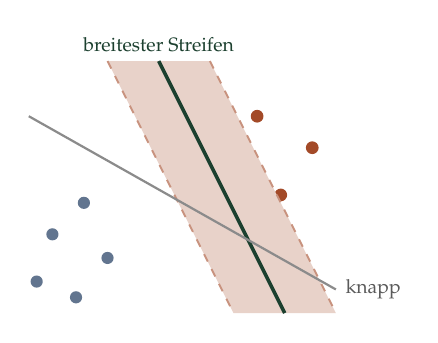
\begin{tikzpicture}[scale=1.0]
\foreach \x/\y in {0.4/0.5,0.9/0.3,0.6/1.1,1.3/0.8,1.0/1.5}
  \fill[tief!70] (\x,\y) circle (2.2pt);
\foreach \x/\y in {3.0/2.0,3.5/1.6,3.2/2.6,3.9/2.2,2.7/2.9}
  \fill[akzent] (\x,\y) circle (2.3pt);
\fill[akzent!25] (1.3,3.3) -- (2.6,3.3) -- (4.2,0.1) -- (2.9,0.1) -- cycle;
\draw[akzent!60, line width=0.7pt, dashed] (1.3,3.3) -- (2.9,0.1);
\draw[akzent!60, line width=0.7pt, dashed] (2.6,3.3) -- (4.2,0.1);
\draw[gruen!60!black, line width=1.3pt] (1.95,3.3) -- (3.55,0.1);
\draw[grau!70, line width=0.8pt] (0.3,2.6) -- (4.2,0.4);
\node[font=\scriptsize, color=gruen!60!black, anchor=south] at (1.95,3.3) {breitester Streifen};
\node[font=\scriptsize, color=grau, anchor=west] at (4.2,0.4) {knapp};
\end{tikzpicture}
\end{center}

\begin{center}
\begin{minipage}{0.9\textwidth}
\textbf{Man wähle die Gerade, die von beiden Gruppen am weitesten entfernt ist.}
\end{minipage}
\end{center}

\begin{center}
\begin{minipage}{0.88\textwidth}
\kursiv{Der Gedanke: Neue Patienten streuen etwas um die gesehenen. \textbf{Eine Grenze, die knapp an einem Trainingspunkt vorbeiführt, ordnet dessen Nachbarn womöglich falsch ein} --- eine Grenze mit breitem Abstand nicht. Satz 5.3 hatte bereits gezeigt, dass der Abstand $\gamma$ über die Schwierigkeit entscheidet; hier wird er zum Ziel.}
\end{minipage}
\end{center}
\end{merksatz}

\begin{definition}
\boxtitelm{Definition 6.1 --- der Rand}
Für eine Gerade $\vek w^{\!\top}\vek x + b = 0$ ist der Abstand eines Punktes $\vek x_i$ mit Etikett $t_i \in \{-1,+1\}$ von ihr
\[ \frac{t_i\,(\vek w^{\!\top}\vek x_i + b)}{\|\vek w\|} . \]
Der \Begriff{Rand} ist der kleinste dieser Abstände.
\end{definition}

\begin{merksatz}
\boxtitel{Das Optimierungsproblem}
Man darf $\vek w$ und $b$ gemeinsam mit einer Zahl multiplizieren, ohne die Gerade zu ändern. Also kann man festlegen, dass für die nächstgelegenen Punkte $t_i(\vek w^{\!\top}\vek x_i+b) = 1$ gilt. Dann ist der Rand $\frac{1}{\|\vek w\|}$, und ihn zu vergrößern heißt $\|\vek w\|$ zu verkleinern:

\[ \min_{\vek w,\,b}\ \tfrac12\|\vek w\|^{2} \qquad\text{unter}\qquad t_i\,(\vek w^{\!\top}\vek x_i + b) \ \ge\ 1 \quad\text{für alle } i \]

\begin{center}
\begin{minipage}{0.9\textwidth}
\textbf{Eine quadratische Zielfunktion unter linearen Nebenbedingungen} --- ein konvexes Problem im Sinne von Band 19, Kapitel~7.
\end{minipage}
\end{center}
\end{merksatz}

\section{Das duale Problem}

\begin{merksatz}
\boxtitel{Satz 6.2 --- die Stützvektoren}
Die Lösung hat die Gestalt
\[ \vek w = \sum_i \alpha_i\,t_i\,\vek x_i \qquad\text{mit}\qquad \alpha_i \ge 0, \quad \sum_i \alpha_i t_i = 0 , \]
und es ist $\alpha_i > 0$ nur für Punkte, die genau auf dem Rand liegen.

\schritt{Beweis}
\kursiv{Die Lagrange-Funktion} (Band 19, Kapitel~9) mit Multiplikatoren $\alpha_i \ge 0$:
\[ L = \tfrac12\|\vek w\|^{2} - \sum_i \alpha_i\bigl[t_i(\vek w^{\!\top}\vek x_i + b) - 1\bigr] \]

\kursiv{Ableiten nach $\vek w$ und null setzen:}
\[ \vek w - \sum_i \alpha_i t_i \vek x_i = \vek 0 \quad\Longrightarrow\quad \vek w = \sum_i \alpha_i t_i \vek x_i \]

\kursiv{Ableiten nach $b$:}
\[ -\sum_i \alpha_i t_i = 0 \]

\kursiv{Komplementärer Schlupf} (Band 19, Satz 9.4): Im Optimum gilt für jedes $i$
\[ \alpha_i\,\bigl[t_i(\vek w^{\!\top}\vek x_i+b) - 1\bigr] = 0 . \]
Liegt ein Punkt nicht auf dem Rand, so ist die Klammer positiv, also $\alpha_i = 0$. $\blacksquare$

\begin{center}
\begin{minipage}{0.9\textwidth}
\textbf{Die Lösung hängt nur von den Punkten auf dem Rand ab --- den \Begriff{Stützvektoren}. Alle anderen könnte man weglassen.}
\end{minipage}
\end{center}

\schritt{Das duale Problem ausgeschrieben}
Setzt man $\vek w$ in $L$ ein, so bleibt
\[ \max_{\vek\alpha}\ \sum_i \alpha_i - \tfrac12\sum_{i,j}\alpha_i\alpha_j\,t_i t_j\,\textcolor{akzent}{\vek x_i^{\!\top}\vek x_j} \]
unter $\alpha_i \ge 0$ und $\sum_i\alpha_i t_i = 0$.

\begin{center}
\begin{minipage}{0.88\textwidth}
\kursiv{\textbf{Man beachte die farbige Stelle: Die Daten kommen nur als Skalarprodukte vor.} Nie wird ein einzelnes $\vek x_i$ gebraucht, nur $\vek x_i^{\!\top}\vek x_j$ für Paare. Auch die Vorhersage für einen neuen Punkt, $\vek w^{\!\top}\vek x + b = \sum_i \alpha_i t_i\,\vek x_i^{\!\top}\vek x + b$, braucht nur Skalarprodukte. Auf dieser Beobachtung beruht der Rest des Kapitels.}
\end{minipage}
\end{center}
\end{merksatz}

\section{Wenn nichts trennt}

\begin{merksatz}
\boxtitel{Der weiche Rand}
Man erlaubt Verstöße, lässt sie aber bezahlen:
\[ \min_{\vek w,\,b}\ \tfrac12\|\vek w\|^{2} + C\sum_i \max\bigl\{0,\ 1 - t_i(\vek w^{\!\top}\vek x_i+b)\bigr\} \]

\schritt{Drei Verluste im Vergleich}
Mit $m = t\,(\vek w^{\!\top}\vek x+b)$ --- positiv heißt richtig, groß heißt sicher:

\begin{center}
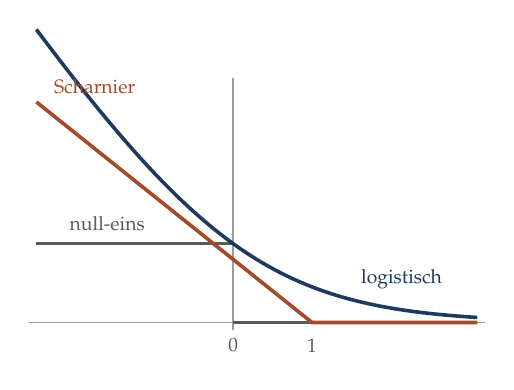
\begin{tikzpicture}[scale=1.0]
\draw[grau!60, line width=0.6pt] (-2.6,0) -- (3.2,0);
\draw[grau!60, line width=0.6pt] (0,-0.1) -- (0,3.1);
\draw[grau, line width=1.2pt] (-2.5,1) -- (0,1); \draw[grau, line width=1.2pt] (0,0) -- (3.1,0);
\draw[akzent, line width=1.3pt] (-2.5,3.5*0.8) -- (1,0) -- (3.1,0);
\draw[tief, line width=1.3pt, smooth, samples=60, domain=-2.5:3.1] plot ({\x}, {ln(1+exp(-\x))/ln(2)});
\node[font=\scriptsize, color=grau, anchor=north] at (1,-0.08) {$1$};
\node[font=\scriptsize, color=grau, anchor=north] at (0,-0.08) {$0$};
\node[font=\scriptsize, color=grau] at (-1.6,1.25) {null-eins};
\node[font=\scriptsize, color=akzent, anchor=west] at (-2.4,3.0) {Scharnier};
\node[font=\scriptsize, color=tief, anchor=west] at (1.5,0.55) {logistisch};
\end{tikzpicture}
\end{center}

\begin{center}
{\small
\renewcommand{\arraystretch}{1.5}
\begin{tabular}{@{}P{2.4cm}P{6.2cm}@{}}
\toprule
\textbf{Null-Eins} & Der eigentliche Fehler. Nicht konvex, nicht stetig --- praktisch nicht zu minimieren.\\
\textbf{Scharnier} & $\max\{0,\,1-m\}$. Konvex. Null, sobald der Punkt sicher richtig liegt.\\
\textbf{Logistisch} & $\ln(1+e^{-m})$. Konvex, glatt. Nie ganz null.\\
\bottomrule
\end{tabular}}
\end{center}

\begin{center}
\begin{minipage}{0.88\textwidth}
\kursiv{Beide konvexen Verluste liegen über dem Null-Eins-Verlust und sind \Begriff{Ersatzverluste} für ihn. \textbf{Das Scharnier kümmert sich nicht um Punkte, die sicher richtig liegen} --- daher die Stützvektoren. Die logistische Kurve kümmert sich um alle, ein wenig --- daher die Wahrscheinlichkeiten. Ansonsten sind sich die beiden Verfahren ähnlicher, als ihre Herkunft vermuten lässt.}
\end{minipage}
\end{center}

\schritt{Die Rolle von $C$}
\begin{center}
{\small
\renewcommand{\arraystretch}{1.5}
\begin{tabular}{@{}P{2.4cm}P{6.2cm}@{}}
\toprule
\textbf{$C$ groß} & Verstöße teuer: schmaler Rand, folgt den Daten --- Varianz.\\
\textbf{$C$ klein} & Verstöße billig: breiter Rand, glatte Grenze --- Verzerrung.\\
\bottomrule
\end{tabular}}
\end{center}

\kursiv{Man erkennt die Kammregression aus Kapitel~4: $\|\vek w\|^{2}$ ist die Strafe, $C$ entspricht $1/\lambda$.}
\end{merksatz}

\section{Der Kerntrick}

\begin{merksatz}
\boxtitel{Eine Abbildung in einen größeren Raum}
Man bilde jeden Punkt ab, etwa
\[ \varphi(x_1, x_2) = \bigl(x_1^{2},\ \sqrt2\,x_1x_2,\ x_2^{2}\bigr) . \]
In diesem neuen Raum sind Grenzen, die im alten Kreise oder Ellipsen waren, gerade Ebenen.

\schritt{Das Skalarprodukt im neuen Raum}
\begin{align*}
\varphi(\vek x)^{\!\top}\varphi(\vek z) &= x_1^{2}z_1^{2} + 2\,x_1x_2z_1z_2 + x_2^{2}z_2^{2}\\
&= (x_1z_1 + x_2z_2)^{2}\\
&= (\vek x^{\!\top}\vek z)^{2}
\end{align*}

\begin{center}
\begin{minipage}{0.9\textwidth}
\textbf{Man kann das Skalarprodukt im großen Raum ausrechnen, ohne je in ihn hineinzugehen.}
\end{minipage}
\end{center}
\end{merksatz}

\begin{definition}
\boxtitelm{Definition 6.3 --- Kern}
Eine Funktion $k(\vek x,\vek z)$ heißt \Begriff{Kern}, wenn es eine Abbildung $\varphi$ gibt mit
\[ k(\vek x,\vek z) = \varphi(\vek x)^{\!\top}\varphi(\vek z) . \]
\end{definition}

\begin{merksatz}
\boxtitel{Der Trick}
Im dualen Problem ersetzt man überall $\vek x_i^{\!\top}\vek x_j$ durch $k(\vek x_i,\vek x_j)$.

\begin{center}
\begin{minipage}{0.9\textwidth}
\textbf{Das Verfahren bleibt linear --- aber in einem Raum, den man nie hinschreibt. Im ursprünglichen Raum wird die Grenze krumm.}
\end{minipage}
\end{center}

\schritt{Gebräuchliche Kerne}
\begin{center}
{\small
\renewcommand{\arraystretch}{1.55}
\begin{tabular}{@{}P{2.4cm}P{3.2cm}P{3.0cm}@{}}
\toprule
\textbf{Name} & \textbf{Formel} & \textbf{Raum}\\
\midrule
linear & $\vek x^{\!\top}\vek z$ & der ursprüngliche\\
Polynom & $(1+\vek x^{\!\top}\vek z)^{d}$ & alle Produkte bis Grad $d$\\
Gauß & $e^{-\gamma\|\vek x-\vek z\|^{2}}$ & \textcolor{akzent}{unendlich-dimensional}\\
\bottomrule
\end{tabular}}
\end{center}

\begin{center}
\begin{minipage}{0.88\textwidth}
\kursiv{Der Gauß-Kern entspricht einem Raum mit unendlich vielen Dimensionen, und trotzdem kostet jede Auswertung nur einen Abstand und eine Exponentialfunktion. \textbf{Anschaulich misst er Ähnlichkeit}: Nahe Punkte haben einen Kern nahe eins, ferne nahe null. Die Vorhersage für einen neuen Patienten ist dann eine gewichtete Abstimmung der Stützvektoren, die ihm ähneln.}
\end{minipage}
\end{center}

\schritt{Satz 6.4 --- Mercer}
Eine symmetrische Funktion $k$ ist genau dann ein Kern, wenn für jede endliche Punktmenge die Matrix $\bigl(k(\vek x_i,\vek x_j)\bigr)_{i,j}$ positiv semidefinit ist.

\begin{center}
\begin{minipage}{0.88\textwidth}
\kursiv{Der Beweis braucht die Spektraltheorie kompakter Operatoren aus Band 13, Kapitel~13; wir verzichten auf ihn --- die zweite Auslassung dieses Bandes. \textbf{Der Satz ist die Garantie, dass man einen Kern benutzen darf, ohne $\varphi$ zu kennen}: Es genügt, die Matrix zu prüfen.}
\end{minipage}
\end{center}
\end{merksatz}

\section{Der Leitfall gerechnet}

\begin{merksatz}
\boxtitel{Dreihundert Patienten, geprüft an zwanzigtausend}
\begin{center}
{\small
\renewcommand{\arraystretch}{1.5}
\begin{tabular}{@{}P{3.6cm}P{2.0cm}P{2.2cm}@{}}
\toprule
\textbf{Verfahren} & \textbf{Fehler} & \textbf{Trennschärfe}\\
\midrule
nie warnen & $20{,}2\,\%$ & ---\\
linear, logistisch & $11{,}8\,\%$ & $0{,}874$\\
linear, Stützvektoren & $10{,}0\,\%$ & ---\\
Gauß-Kern & $\mathbf{3{,}0\,\%}$ & $0{,}975$\\
logistisch mit $(T-37)^{2}$ & $3{,}2\,\%$ & $\mathbf{0{,}994}$\\
\bottomrule
\end{tabular}}
\end{center}

\begin{center}
\begin{minipage}{0.9\textwidth}
\textbf{Der Gauß-Kern findet die krumme Grenze von selbst. Ein einziges gut gewähltes Merkmal leistet dasselbe.}
\end{minipage}
\end{center}

\schritt{Die Stützvektoren}
Von $300$ Patienten dienen $72$ als Stützvektoren --- knapp ein Viertel.

\schritt{Was die letzte Zeile lehrt}
\begin{center}
\begin{minipage}{0.88\textwidth}
\kursiv{Das Merkmal $(T-37)^{2}$ --- der quadrierte Abstand von der Normaltemperatur --- ist medizinisches Wissen in einer Zahl. \textbf{Es macht aus dem krummen Problem ein gerades}, und die einfache logistische Regression löst es danach mindestens so gut wie der Kern. Zudem bleibt sie deutbar: Man kann ablesen, wie stark die Abweichung von $37$ Grad wirkt. Der Kern kann das nicht.}
\end{minipage}
\end{center}

\begin{center}
\begin{minipage}{0.88\textwidth}
\kursiv{Das ist Satz 1.5 in einer neuen Gestalt: \textbf{Wer die richtige Annahme kennt, sollte sie hineinstecken, statt sie suchen zu lassen.} Der Kern ist das Mittel der Wahl, wenn man sie \kursiv{nicht} kennt --- und dann zahlt man dafür mit Daten, Rechenzeit und Deutbarkeit.}
\end{minipage}
\end{center}
\end{merksatz}

\section{Der Bruchfall}

\begin{warnung}
\boxtitelr{Was der Kern kostet}
\begin{center}
{\small
\renewcommand{\arraystretch}{1.52}
\begin{tabular}{@{}P{2.8cm}P{5.8cm}@{}}
\toprule
\textbf{Rechen\-aufwand} & Die Kernmatrix hat $n^{2}$ Einträge. Bei einer Million Patienten sind das $10^{12}$ --- nicht mehr zu speichern.\\
\textbf{Zwei Stellgrößen} & $C$ und die Kernbreite $\gamma$ müssen durch Kreuzvalidierung gewählt werden --- mit allen Gefahren aus Kapitel~3.\\
\textbf{Einheiten} & Der Gauß-Kern misst Abstände. Ohne Normierung dominiert die Herzfrequenz (Größenordnung $100$) die Temperatur (Größenordnung $1$).\\
\textbf{Keine Wahrscheinlichkeit} & Die Ausgabe ist ein Abstand zur Grenze, keine Wahrscheinlichkeit. Man muss sie nachträglich umrechnen.\\
\bottomrule
\end{tabular}}
\end{center}

\schritt{Zur dritten Zeile}
\begin{center}
\begin{minipage}{0.88\textwidth}
\kursiv{Ohne Normierung wäre ein Unterschied von zwei Schlägen pro Minute so groß wie einer von zwei Grad Temperatur --- medizinisch absurd. \textbf{Der Kern kennt keine Einheiten}; er sieht Zahlen. Die Normierung ist hier keine Formsache, sondern entscheidet, welches Merkmal überhaupt zählt.}
\end{minipage}
\end{center}

\schritt{Zur vierten Zeile}
\begin{center}
\begin{minipage}{0.88\textwidth}
\kursiv{Nach Kapitel~1 braucht man für eine kostenbewusste Entscheidung eine Wahrscheinlichkeit. \textbf{Die Stützvektormaschine liefert sie nicht} --- ihr Verlust kümmert sich nicht um Punkte jenseits des Randes und hat daher keine Grundlage, Sicherheit abzustufen. Man kann eine logistische Kurve nachträglich anpassen, aber das ist ein zweites Modell auf dem ersten, mit eigenem Fehler.}
\end{minipage}
\end{center}
\end{warnung}

\section{Übungsaufgaben}

\begin{aufgabe}
\boxtitel{Aufgabe 6.1 --- Der breiteste Streifen in einer Dimension}
Die Laktatwerte aus Aufgabe 5.3: $1{,}0$ und $1{,}5$ ohne, $2{,}5$ und $3{,}0$ mit Sepsis. Bestimmen Sie $w$, $b$, den Rand und die Multiplikatoren.

\loesung
\schritt{Schritt 1 --- Die Lage der Grenze}
Die engsten Punkte verschiedener Gruppen sind $1{,}5$ und $2{,}5$. Die Grenze liegt in der Mitte:
\[ x^{*} = \frac{1{,}5+2{,}5}{2} = 2{,}0 \]

\schritt{Schritt 2 --- $w$ und $b$}
Die Stützvektoren erfüllen die Nebenbedingung mit Gleichheit:
\[ w\cdot2{,}5 + b = +1, \qquad w\cdot1{,}5 + b = -1 \]
Subtrahieren: $w = 2$. Einsetzen: $b = 1 - 5 = -4$.

\kursiv{Probe:} $2\cdot2{,}0 - 4 = 0$ --- die Grenze liegt bei $2{,}0$. \checkmark

\schritt{Schritt 3 --- Der Rand}
\[ \frac{1}{|w|} = \frac12 = 0{,}5 \]
--- genau der halbe Abstand zwischen $1{,}5$ und $2{,}5$. \checkmark

\schritt{Schritt 4 --- Die übrigen Punkte}
\begin{center}
{\small
\renewcommand{\arraystretch}{1.46}
\begin{tabular}{@{}P{1.4cm}P{1.0cm}P{2.6cm}P{2.4cm}@{}}
\toprule
$x$ & $t$ & $t\,(wx+b)$ & \\
\midrule
$1{,}0$ & $-1$ & $-(2-4) = 2$ & jenseits\\
$1{,}5$ & $-1$ & $-(3-4) = 1$ & \textcolor{akzent}{auf dem Rand}\\
$2{,}5$ & $+1$ & $5-4 = 1$ & \textcolor{akzent}{auf dem Rand}\\
$3{,}0$ & $+1$ & $6-4 = 2$ & jenseits\\
\bottomrule
\end{tabular}}
\end{center}

\schritt{Schritt 5 --- Die Multiplikatoren}
Nur die Stützvektoren haben $\alpha > 0$. Aus $\sum\alpha_i t_i = 0$ folgt $\alpha_{1{,}5} = \alpha_{2{,}5} =: \alpha$. Aus $w = \sum\alpha_i t_i x_i$:
\[ 2 = \alpha\cdot(+1)\cdot2{,}5 + \alpha\cdot(-1)\cdot1{,}5 = \alpha\cdot1{,}0 \quad\Longrightarrow\quad \alpha = 2 \]

\schritt{Schritt 6 --- Eine Probe über eine Identität}
Im Optimum gilt $\|\vek w\|^{2} = \sum_i\alpha_i$.

\kursiv{Warum:} $\|\vek w\|^{2} = \vek w^{\!\top}\sum\alpha_i t_i\vek x_i = \sum\alpha_i\,t_i\vek w^{\!\top}\vek x_i$. Auf dem Rand ist $t_i\vek w^{\!\top}\vek x_i = 1 - t_i b$, also $\sum\alpha_i(1-t_ib) = \sum\alpha_i - b\sum\alpha_it_i = \sum\alpha_i$.

\[ \|w\|^{2} = 4, \qquad \sum\alpha_i = 2+2 = 4 \quad \checkmark \]

\begin{center}
\begin{minipage}{0.88\textwidth}
\kursiv{\textbf{Die Punkte bei $1{,}0$ und $3{,}0$ spielen keine Rolle.} Man könnte sie verschieben, solange sie jenseits des Randes bleiben, und die Lösung änderte sich nicht. Die logistische Regression dagegen würde jede Verschiebung spüren.}
\end{minipage}
\end{center}
\end{aufgabe}

\begin{aufgabe}
\boxtitel{Aufgabe 6.2 --- Den Kerntrick nachrechnen}
Prüfen Sie für $\vek x = (1,2)$ und $\vek z = (3,1)$, dass $(\vek x^{\!\top}\vek z)^{2} = \varphi(\vek x)^{\!\top}\varphi(\vek z)$ mit $\varphi$ aus Abschnitt 6.5.

\loesung
\schritt{Schritt 1 --- Der Kern}
\[ \vek x^{\!\top}\vek z = 1\cdot3 + 2\cdot1 = 5, \qquad (\vek x^{\!\top}\vek z)^{2} = 25 \]

\schritt{Schritt 2 --- Die Abbildung}
\[ \varphi(\vek x) = \bigl(1^{2},\ \sqrt2\cdot1\cdot2,\ 2^{2}\bigr) = (1;\ 2{,}828;\ 4) \]
\[ \varphi(\vek z) = \bigl(3^{2},\ \sqrt2\cdot3\cdot1,\ 1^{2}\bigr) = (9;\ 4{,}243;\ 1) \]

\schritt{Schritt 3 --- Das Skalarprodukt}
\[ 1\cdot9 + 2{,}828\cdot4{,}243 + 4\cdot1 = 9 + 12{,}00 + 4 = 25 \quad \checkmark \]

\kursiv{Exakt:} $\sqrt2\cdot2\cdot\sqrt2\cdot3 = 2\cdot6 = 12$.

\schritt{Schritt 4 --- Der Aufwand}
\begin{center}
{\small
\renewcommand{\arraystretch}{1.5}
\begin{tabular}{@{}P{3.4cm}P{2.2cm}P{2.2cm}@{}}
\toprule
\textbf{Grad, Dimension} & \textbf{über $\varphi$} & \textbf{über $k$}\\
\midrule
$2$, $2$ & $3$ Einträge & $2$ Produkte\\
$2$, $100$ & $5050$ & $100$\\
$5$, $100$ & $\approx 10^{8}$ & $100$\\
\bottomrule
\end{tabular}}
\end{center}

\begin{center}
\begin{minipage}{0.88\textwidth}
\kursiv{Bei Grad $5$ und $100$ Merkmalen hätte $\varphi$ fast hundert Millionen Einträge --- alle Produkte von bis zu fünf Merkmalen. \textbf{Der Kern braucht dafür $100$ Multiplikationen und eine Potenz.} Das ist der ganze Trick: Die Rechnung hängt von der Dimension der Daten ab, nicht von der des Raumes, in dem man trennt.}
\end{minipage}
\end{center}
\end{aufgabe}

\begin{aufgabe}
\boxtitel{Aufgabe 6.3 --- Das XOR-Problem}
Vier Punkte: $(1,1)$ und $(-1,-1)$ mit Etikett $+1$, $(1,-1)$ und $(-1,1)$ mit Etikett $-1$. Zeigen Sie, dass keine Gerade trennt, und finden Sie eine Trennung mit $\varphi$.

\loesung
\schritt{Schritt 1 --- Keine Gerade trennt}
Angenommen, $w_1x_1 + w_2x_2 + b$ hätte das richtige Vorzeichen an allen vier Punkten:
\begin{align*}
w_1 + w_2 + b &> 0 & -w_1 - w_2 + b &> 0\\
w_1 - w_2 + b &< 0 & -w_1 + w_2 + b &< 0
\end{align*}
Addiert man die beiden Ungleichungen der oberen Zeile, so folgt $2b > 0$. Addiert man die der unteren Zeile, so folgt $2b < 0$. \textbf{Widerspruch.}

\schritt{Schritt 2 --- In den neuen Raum}
\begin{center}
{\small
\renewcommand{\arraystretch}{1.48}
\begin{tabular}{@{}P{2.0cm}P{1.0cm}P{3.6cm}@{}}
\toprule
$\vek x$ & $t$ & $\varphi(\vek x) = (x_1^{2},\ \sqrt2x_1x_2,\ x_2^{2})$\\
\midrule
$(1,1)$ & $+1$ & $(1;\ +\sqrt2;\ 1)$\\
$(-1,-1)$ & $+1$ & $(1;\ +\sqrt2;\ 1)$\\
$(1,-1)$ & $-1$ & $(1;\ -\sqrt2;\ 1)$\\
$(-1,1)$ & $-1$ & $(1;\ -\sqrt2;\ 1)$\\
\bottomrule
\end{tabular}}
\end{center}

\schritt{Schritt 3 --- Die Trennung}
Die mittlere Koordinate allein trennt: positiv bei $+1$, negativ bei $-1$.
\[ \vek w = (0;\ 1;\ 0), \qquad b = 0 \]

\begin{center}
\begin{minipage}{0.9\textwidth}
\textbf{Im neuen Raum trennt eine Ebene. Im alten Raum ist die Grenze das Achsenkreuz $x_1x_2 = 0$.}
\end{minipage}
\end{center}

\schritt{Schritt 4 --- Die klinische Entsprechung}
\begin{center}
\begin{minipage}{0.88\textwidth}
\kursiv{Das XOR-Muster tritt auf, wenn zwei Merkmale nur \kursiv{gemeinsam} wirken --- etwa ein Medikament, das nur bei einer bestimmten Genvariante schadet. \textbf{Einzeln zeigt keines der beiden einen Zusammenhang}, und jedes Verfahren, das Merkmale einzeln prüft, übersieht die Wirkung vollständig. Das ist die Aufgabe, an der Minsky und Papert 1969 das einzelne Perzeptron scheitern ließen.}
\end{minipage}
\end{center}
\end{aufgabe}

\begin{geschichte}
\boxtitelg{Eine Idee aus Moskau, dreißig Jahre unterwegs}
\Person{Wladimir Wapnik} und \Person{Alexei Tscherwonenkis} entwickelten ab den 1960er Jahren in Moskau die Theorie, auf der dieses und das nächste Kapitel beruhen.

\begin{center}
\begin{minipage}{0.9\textwidth}
\kursiv{Die Methode des verallgemeinerten Porträts --- die Trennung mit breitestem Rand --- beschrieben sie 1963. \textbf{Im Westen wurde ihre Arbeit kaum wahrgenommen}, weil sie überwiegend auf Russisch erschien und die Sowjetunion den wissenschaftlichen Austausch beschränkte.}
\end{minipage}
\end{center}

\schritt{Die Auswanderung}
Wapnik ging 1990 in die Vereinigten Staaten, an die Bell Laboratories.

\begin{center}
\begin{minipage}{0.9\textwidth}
\kursiv{Dort verband er 1992 mit \Person{Bernhard Boser} und \Person{Isabelle Guyon} den breitesten Rand mit dem Kerntrick; 1995 kam mit \Person{Corinna Cortes} der weiche Rand hinzu. \textbf{Innerhalb weniger Jahre wurden Stützvektormaschinen zum Standardverfahren} und verdrängten die neuronalen Netze, die damals als schwer zu beherrschen galten.}
\end{minipage}
\end{center}

\schritt{Der Kerntrick ist älter}
\begin{center}
\begin{minipage}{0.9\textwidth}
\kursiv{\Person{Mark Aiserman} und Mitarbeiter hatten Kerne bereits 1964 benutzt, ebenfalls in Moskau, für eine Variante des Perzeptrons. \textbf{Die Idee lag also fast dreißig Jahre bereit}, bevor jemand sie mit der richtigen Zielfunktion verband.}
\end{minipage}
\end{center}

\schritt{Und die Umkehr}
\begin{center}
\begin{minipage}{0.9\textwidth}
\kursiv{Ab 2012 kehrten die Netze zurück und verdrängten ihrerseits die Stützvektormaschinen --- zumindest bei Bildern, Sprache und Text. \textbf{Bei tabellarischen Daten mit wenigen tausend Fällen sind Kernverfahren weiterhin konkurrenzfähig}, und ihre Theorie ist ungleich besser verstanden.}
\end{minipage}
\end{center}
\end{geschichte}

\begin{forschung}
\boxtitelp{Kerne heute}
\begin{center}
{\small
\renewcommand{\arraystretch}{1.45}
\begin{tabular}{@{}P{2.8cm}P{5.4cm}@{}}
\toprule
\textbf{Große Daten} & Näherungen, die die Kernmatrix nie vollständig bilden.\\
\textbf{Gaußprozesse} & Kerne mit Wahrscheinlichkeitsdeutung --- samt Unsicherheit.\\
\textbf{Netze als Kerne} & Sehr breite Netze verhalten sich wie Kernverfahren.\\
\bottomrule
\end{tabular}}
\end{center}

\schritt{Zur zweiten Zeile}
\begin{center}
\begin{minipage}{0.88\textwidth}
\kursiv{Ein Gaußprozess benutzt denselben Kern, deutet ihn aber als Kovarianz zwischen den Werten an verschiedenen Stellen. \textbf{Er liefert zu jeder Vorhersage eine Unsicherheit} --- und die wird groß, wo keine Daten liegen. Das ist genau, was der Bruchfall von Kapitel~2 vermisste: ein Verfahren, das weiß, wo es nichts weiß.}
\end{minipage}
\end{center}

\schritt{Zur dritten Zeile}
\begin{center}
\begin{minipage}{0.88\textwidth}
\kursiv{2018 wurde gezeigt, dass ein neuronales Netz im Grenzfall unendlicher Breite genau einem Kernverfahren entspricht --- mit einem Kern, den man aus dem Aufbau des Netzes ausrechnen kann. \textbf{Das ist eine der wenigen Brücken zwischen der Theorie dieses Teils und den tiefen Netzen} aus Kapitel~14. Sie trägt allerdings nicht weit: Die erfolgreichen Netze sind gerade nicht unendlich breit, und ihr Vorteil liegt vermutlich in dem, was dieser Grenzfall wegwirft.}
\end{minipage}
\end{center}
\end{forschung}

\begin{merksatz}
\boxtitel{Was Sie jetzt können}
\begin{center}
\renewcommand{\arraystretch}{1.5}
\begin{tabular}{@{}P{3.0cm}P{5.6cm}@{}}
\toprule
\textbf{Definition 6.1} & Rand $= 1/\|\vek w\|$\\
\textbf{Satz 6.2} & nur die Stützvektoren zählen\\
\textbf{Scharnierverlust} & konvexer Ersatz für Null-Eins\\
\textbf{Kerntrick} & Skalarprodukt ersetzen, Raum nie betreten\\
\textbf{Der Leitfall} & ein gutes Merkmal schlägt den Kern\\
\bottomrule
\end{tabular}
\end{center}

\begin{center}
\begin{minipage}{0.88\textwidth}
\kursiv{Damit endet Teil~II. Seine Verfahren funktionieren --- aber warum? Wie viele Daten braucht man, damit der Trainingsfehler etwas über den Testfehler sagt? Teil~III gibt die Antwort, und sie hängt an einer einzigen Zahl.}
\end{minipage}
\end{center}
\end{merksatz}

\part{Die Theorie}

\chapter{Wie viele Beispiele man braucht}

\section{Die Frage}

\begin{merksatz}
\boxtitel{Wann sagt der Trainingsfehler etwas?}
Kapitel~2 zeigte, dass der Trainingsfehler zu optimistisch ist, und gab für lineare Modelle mit $p$ Parametern die Korrektur $2\sigma^{2}p/n$ an. Kapitel~3 zeigte, wie man den Testfehler mit zurückgehaltenen Daten schätzt.

\begin{center}
\begin{minipage}{0.9\textwidth}
\textbf{Offen ist die grundsätzliche Frage: Unter welchen Bedingungen liegt der Trainingsfehler \kursiv{garantiert} nahe am Testfehler --- und wie viele Beispiele braucht man dafür?}
\end{minipage}
\end{center}

\begin{center}
\begin{minipage}{0.88\textwidth}
\kursiv{Die Antwort muss für \kursiv{jede} Verteilung gelten, denn wir kennen die Verteilung nicht. \textbf{Und sie muss für die gewählte Regel gelten}, obwohl diese gerade deshalb gewählt wurde, weil sie auf den Trainingsdaten gut aussah --- das ist die Schwierigkeit, an der Kapitel~3 den Betrug festmachte.}
\end{minipage}
\end{center}
\end{merksatz}

\begin{definition}
\boxtitelm{Definition 7.1 --- wahrscheinlich ungefähr richtig}
Eine Klasse $\Hyp$ von Regeln heißt \Begriff{lernbar}, wenn es zu jeder Genauigkeit $\varepsilon > 0$ und jeder Irrtumswahrscheinlichkeit $\delta > 0$ eine Stichprobengröße $n(\varepsilon,\delta)$ gibt, so dass für \kursiv{jede} Verteilung gilt:

\begin{center}
\begin{minipage}{0.88\textwidth}
Mit Wahrscheinlichkeit mindestens $1-\delta$ liegt das Risiko der gelernten Regel höchstens um $\varepsilon$ über dem der besten Regel in $\Hyp$.
\end{minipage}
\end{center}
\end{definition}

\begin{merksatz}
\boxtitel{Die beiden Toleranzen}
\begin{center}
{\small
\renewcommand{\arraystretch}{1.55}
\begin{tabular}{@{}P{2.8cm}P{5.8cm}@{}}
\toprule
\textbf{Ungefähr} & $\varepsilon$: Man verlangt nicht das beste Ergebnis, sondern eines, das nahe daran liegt.\\
\textbf{Wahrscheinlich} & $\delta$: Man verlangt es nicht sicher, denn eine unglückliche Stichprobe kann jeden täuschen.\\
\bottomrule
\end{tabular}}
\end{center}

\begin{center}
\begin{minipage}{0.88\textwidth}
\kursiv{Beide Toleranzen sind unvermeidlich. \textbf{Mit endlich vielen Beispielen ist keine exakte Aussage möglich}, und keine sichere --- es könnte ja zufällig nur gesunde Patienten mit hohem Laktat gezogen haben. Der Begriff heißt nach den englischen Anfangsbuchstaben PAC, \enquote{probably approximately correct}.}
\end{minipage}
\end{center}
\end{merksatz}

\section{Endlich viele Regeln}

\begin{merksatz}
\boxtitel{Der einfachste Fall}
Die Laktatschwelle werde nur in Schritten von $0{,}1$ zwischen $0$ und $10$ mmol/l gewählt --- das sind $|\Hyp| = 101$ Regeln.

\schritt{Satz 7.2 --- wenn eine Regel fehlerfrei ist}
Gibt es in $\Hyp$ eine Regel mit Risiko null, und wählt man eine Regel, die alle Trainingsdaten richtig einordnet, so hat sie mit Wahrscheinlichkeit mindestens $1-\delta$ ein Risiko von höchstens $\varepsilon$, sobald
\[ n \ \ge\ \frac{\ln|\Hyp| + \ln(1/\delta)}{\varepsilon} . \]

\schritt{Beweis}
Nenne eine Regel \kursiv{schlecht}, wenn ihr Risiko größer als $\varepsilon$ ist.

\kursiv{Eine einzelne schlechte Regel} ordnet jeden Patienten mit Wahrscheinlichkeit höchstens $1-\varepsilon$ richtig ein. Alle $n$ unabhängig gezogenen richtig einzuordnen, gelingt ihr mit Wahrscheinlichkeit höchstens
\[ (1-\varepsilon)^{n} \ \le\ e^{-\varepsilon n} , \]
denn $1-\varepsilon \le e^{-\varepsilon}$ (Band 3, die Tangente an die Exponentialfunktion).

\kursiv{Irgendeine schlechte Regel} täuscht mit Wahrscheinlichkeit höchstens der Summe über alle --- höchstens $|\Hyp|$ Stück:
\[ \Pr[\text{eine schlechte Regel ist fehlerfrei}] \ \le\ |\Hyp|\,e^{-\varepsilon n} . \]

\kursiv{Soll das höchstens $\delta$ sein}, so braucht man
\[ |\Hyp|\,e^{-\varepsilon n} \le \delta \quad\Longleftrightarrow\quad \varepsilon n \ge \ln|\Hyp| + \ln(1/\delta) . \]
$\blacksquare$

\begin{center}
\begin{minipage}{0.9\textwidth}
\textbf{Die Zahl der Regeln geht nur logarithmisch ein.} Verdoppelt man sie, braucht man nur $\ln2/\varepsilon$ Beispiele mehr.
\end{minipage}
\end{center}
\end{merksatz}

\begin{merksatz}
\boxtitel{Satz 7.3 --- wenn keine Regel fehlerfrei ist}
Im allgemeinen Fall liegt mit Wahrscheinlichkeit mindestens $1-\delta$ der Trainingsfehler \kursiv{jeder} Regel in $\Hyp$ höchstens $\varepsilon$ neben ihrem Risiko, sobald
\[ n \ \ge\ \frac{\ln|\Hyp| + \ln(2/\delta)}{2\,\varepsilon^{2}} . \]

\schritt{Der Hilfssatz}
Die \Begriff{Ungleichung von Hoeffding} besagt: Für den Anteil $\hat p$ von Erfolgen in $n$ unabhängigen Versuchen mit Erfolgswahrscheinlichkeit $p$ gilt
\[ \Pr\bigl[|\hat p - p| > \varepsilon\bigr] \ \le\ 2\,e^{-2n\varepsilon^{2}} . \]

\begin{center}
\begin{minipage}{0.88\textwidth}
\kursiv{Wir verwenden sie ohne Beweis --- die dritte Auslassung dieses Bandes; die Fundstelle ist Shalev-Shwartz und Ben-David\zit{24}, Anhang B. \textbf{Sie ist eine schärfere Fassung des Gesetzes der großen Zahlen}: Nicht nur geht die Abweichung gegen null, sondern die Wahrscheinlichkeit einer großen Abweichung fällt exponentiell.}
\end{minipage}
\end{center}

\schritt{Beweis von Satz 7.3}
Für eine feste Regel ist der Trainingsfehler ein Anteil wie $\hat p$. Nach Hoeffding weicht er mit Wahrscheinlichkeit höchstens $2e^{-2n\varepsilon^{2}}$ um mehr als $\varepsilon$ ab. Für alle Regeln zusammen höchstens das $|\Hyp|$-fache. Gleichsetzen mit $\delta$ und nach $n$ auflösen. $\blacksquare$

\schritt{Der Vergleich}
Für $|\Hyp| = 101$ und $\delta = 0{,}05$:
\begin{center}
{\small
\renewcommand{\arraystretch}{1.5}
\begin{tabular}{@{}P{1.6cm}P{2.8cm}P{2.8cm}@{}}
\toprule
$\varepsilon$ & \textbf{eine fehlerfrei} & \textbf{allgemein}\\
\midrule
$0{,}05$ & $153$ & $1661$\\
$0{,}01$ & $762$ & $41\,520$\\
\bottomrule
\end{tabular}}
\end{center}

\begin{center}
\begin{minipage}{0.9\textwidth}
\textbf{Im allgemeinen Fall geht die Genauigkeit quadratisch ein} --- zehnmal genauer kostet hundertmal mehr Daten.
\end{minipage}
\end{center}

\begin{center}
\begin{minipage}{0.88\textwidth}
\kursiv{Das ist dieselbe Wurzel aus $n$, die in Band 17 die Breite jedes Vertrauensintervalls bestimmt. \textbf{Der fehlerfreie Fall ist schneller, weil eine einzige Fehleinordnung eine schlechte Regel bereits verrät} --- im allgemeinen Fall muss man den Fehleranteil genau genug messen, und das kostet die übliche statistische Genauigkeit.}
\end{minipage}
\end{center}
\end{merksatz}

\section{Unendlich viele Regeln}

\begin{merksatz}
\boxtitel{Das Problem}
Lässt man jede Laktatschwelle zu, nicht nur Zehntelschritte, so ist $|\Hyp| = \infty$, und die Schranken aus Abschnitt 7.2 sagen nichts mehr.

\begin{center}
\begin{minipage}{0.9\textwidth}
\textbf{Und doch ist offensichtlich, dass sich eine Schwelle aus Daten lernen lässt.}
\end{minipage}
\end{center}

\schritt{Der Ausweg}
Auf $n$ gegebenen Patienten erzeugen alle unendlich vielen Schwellen nur endlich viele \kursiv{verschiedene Einteilungen} --- höchstens $n+1$, je nachdem, zwischen welchen beiden Messwerten die Schwelle liegt.

\begin{center}
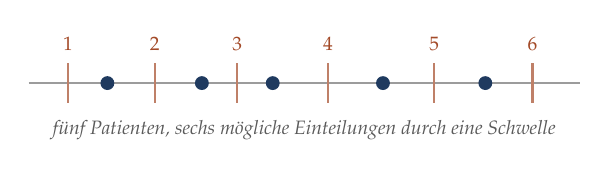
\begin{tikzpicture}[scale=1.0]
\draw[grau!60, line width=0.7pt] (0,0) -- (7,0);
\foreach \x in {1,2.2,3.1,4.5,5.8} \fill[tief] (\x,0) circle (2.5pt);
\foreach \x/\l in {0.5/1,1.6/2,2.65/3,3.8/4,5.15/5,6.4/6}
  { \draw[akzent!70, line width=0.8pt] (\x,-0.25) -- (\x,0.25); \node[font=\scriptsize, color=akzent] at (\x,0.5) {\l}; }
\node[font=\scriptsize\itshape, color=grau] at (3.5,-0.6) {fünf Patienten, sechs mögliche Einteilungen durch eine Schwelle};
\end{tikzpicture}
\end{center}

\begin{center}
\begin{minipage}{0.88\textwidth}
\kursiv{\textbf{Entscheidend ist nicht, wie viele Regeln es gibt, sondern wie viele verschiedene Dinge sie auf den Daten tun können.} Unendlich viele Schwellen verhalten sich auf fünf Patienten wie sechs Regeln.}
\end{minipage}
\end{center}
\end{merksatz}

\begin{definition}
\boxtitelm{Definition 7.4 --- zerschmettern, VC-Dimension}
Eine Klasse $\Hyp$ \Begriff{zerschmettert} eine Punktmenge, wenn sie jede der $2^{m}$ möglichen Einteilungen dieser $m$ Punkte in zwei Gruppen erzeugen kann.

Die \Begriff{VC-Dimension} von $\Hyp$ ist die größte Zahl $d$, für die es eine Menge von $d$ Punkten gibt, die $\Hyp$ zerschmettert.
\end{definition}

\begin{merksatz}
\boxtitel{Beispiele}
\begin{center}
{\small
\renewcommand{\arraystretch}{1.55}
\begin{tabular}{@{}P{3.4cm}P{1.4cm}P{3.4cm}@{}}
\toprule
\textbf{Klasse} & $d$ & \textbf{Begründung}\\
\midrule
Schwellen auf $\R$ & $1$ & zwei Punkte: \enquote{links ja, rechts nein} unmöglich\\
Intervalle auf $\R$ & $2$ & Aufgabe 7.2\\
Halbebenen im $\R^{2}$ & $3$ & Aufgabe 7.3\\
Halbräume im $\R^{p}$ & $p+1$ & allgemein\\
Stützvektoren mit Gauß-Kern & $\infty$ & jede Punktmenge trennbar\\
$\operatorname{sign}\sin(\omega x)$ & $\infty$ & \textcolor{akzent}{ein einziger Parameter!}\\
\bottomrule
\end{tabular}}
\end{center}

\begin{center}
\begin{minipage}{0.88\textwidth}
\kursiv{\textbf{Die letzte Zeile zerstört die Vorstellung, man könne Parameter einfach zählen.} Die Familie $\sin(\omega x)$ hat nur den Parameter $\omega$ --- und kann doch durch geeignet hohe Frequenz jede Einteilung beliebig vieler geschickt gelegter Punkte erzeugen. Die VC-Dimension misst nicht die Zahl der Stellschrauben, sondern die Ausdrucksfähigkeit.}
\end{minipage}
\end{center}

\begin{center}
\begin{minipage}{0.88\textwidth}
\kursiv{Die vorletzte Zeile ist ebenso wichtig: Der Gauß-Kern aus Kapitel~6 hat unendliche VC-Dimension. \textbf{Nach der Theorie dieses Kapitels dürfte er gar nicht lernen} --- und tut es doch. Kapitel~8 löst den Widerspruch über den Rand.}
\end{minipage}
\end{center}
\end{merksatz}

\section{Der Fundamentalsatz}

\begin{merksatz}
\boxtitel{Satz 7.5 --- Sauer, 1972}
Hat $\Hyp$ die VC-Dimension $d$, so erzeugt $\Hyp$ auf $n$ Punkten höchstens
\[ \sum_{i=0}^{d}\binom{n}{i} \ \le\ \left(\frac{e\,n}{d}\right)^{d} \]
verschiedene Einteilungen.

\begin{center}
{\small
\renewcommand{\arraystretch}{1.46}
\begin{tabular}{@{}P{1.4cm}P{2.2cm}P{3.0cm}@{}}
\toprule
$n$ & $2^{n}$ & \textbf{Schranke bei $d = 2$}\\
\midrule
$3$ & $8$ & $7$\\
$5$ & $32$ & $16$\\
$10$ & $1024$ & $56$\\
$20$ & $1\,048\,576$ & $211$\\
\bottomrule
\end{tabular}}
\end{center}

\begin{center}
\begin{minipage}{0.9\textwidth}
\textbf{Sobald $n$ die VC-Dimension übersteigt, springt das Wachstum von exponentiell auf polynomial.}
\end{minipage}
\end{center}

\begin{center}
\begin{minipage}{0.88\textwidth}
\kursiv{Der Beweis ist eine Induktion über $n$ und $d$ --- übersichtlich, aber länger als der Platz hier erlaubt; wir verzichten auf ihn, die vierte Auslassung. \textbf{Für Intervalle ($d = 2$) wird die Schranke genau erreicht}: $1 + n + \binom n2$ Einteilungen --- keine, ein Punkt, ein zusammenhängendes Stück.}
\end{minipage}
\end{center}
\end{merksatz}

\begin{merksatz}
\boxtitel{Satz 7.6 --- Vapnik und Tscherwonenkis, 1971}
Eine Klasse ist genau dann lernbar, wenn ihre VC-Dimension endlich ist. In diesem Fall gilt mit Wahrscheinlichkeit mindestens $1-\delta$ für jede Regel $h \in \Hyp$:
\[ \Risk(h) \ \le\ \hat\Risk(h) + \sqrt{\frac{8}{n}\left(d\,\ln\frac{2e\,n}{d} + \ln\frac4\delta\right)} . \]

\begin{center}
\begin{minipage}{0.9\textwidth}
\textbf{An die Stelle von $\ln|\Hyp|$ tritt im Wesentlichen $d\ln n$.} Endlich viele Einteilungen genügen --- unendlich viele Regeln schaden nicht.
\end{minipage}
\end{center}

\begin{center}
\begin{minipage}{0.88\textwidth}
\kursiv{Der Beweis führt über einen Kunstgriff, die \enquote{Symmetrisierung}: Man vergleicht zwei unabhängige Stichproben miteinander statt eine Stichprobe mit der unbekannten Verteilung. Dadurch hat man es nur mit endlich vielen Punkten zu tun, und Satz 7.5 greift. \textbf{Wir verzichten auf ihn} --- die fünfte Auslassung; die Fundstelle ist Shalev-Shwartz und Ben-David\zit{24}, Kapitel~28.}
\end{minipage}
\end{center}

\schritt{Die beiden Richtungen}
\begin{center}
{\small
\renewcommand{\arraystretch}{1.5}
\begin{tabular}{@{}P{2.6cm}P{6.0cm}@{}}
\toprule
\textbf{$d$ endlich} & Die Schranke geht mit wachsendem $n$ gegen null --- man lernt.\\
\textbf{$d$ unendlich} & Für jedes $n$ gibt es eine Verteilung, auf der jedes Verfahren versagt.\\
\bottomrule
\end{tabular}}
\end{center}

\begin{center}
\begin{minipage}{0.88\textwidth}
\kursiv{Die zweite Zeile ist Satz 1.5 in schärferer Form. \textbf{Bei unendlicher VC-Dimension kann man immer noch auswendig lernen} --- jede Einteilung der Trainingsdaten ist erreichbar ---, und damit ist nichts über ungesehene Daten gesagt.}
\end{minipage}
\end{center}
\end{merksatz}

\section{Der Bruchfall}

\begin{warnung}
\boxtitelr{Wie lose die Schranke ist}
Für die Laktatschwelle ($d = 1$, $\delta = 0{,}05$):

\begin{center}
{\small
\renewcommand{\arraystretch}{1.5}
\begin{tabular}{@{}P{1.8cm}P{2.4cm}P{2.8cm}@{}}
\toprule
$n$ & \textbf{Schranke} & \textbf{tatsächlich (95\,\%)}\\
\midrule
$100$ & $0{,}924$ & $0{,}041$\\
$1000$ & $0{,}322$ & $0{,}012$\\
$100\,000$ & $0{,}038$ & ---\\
\bottomrule
\end{tabular}}
\end{center}
\kursiv{Die rechte Spalte: Abstand zwischen Test- und Trainingsfehler der besten Schwelle, $500$ Stichproben aus der Verteilung von Kapitel~1, $95$-Prozent-Quantil.}

\begin{center}
\begin{minipage}{0.9\textwidth}
\textbf{Bei tausend Patienten garantiert die Schranke eine Genauigkeit von $32$ Prozentpunkten. Tatsächlich liegt sie bei gut einem.}
\end{minipage}
\end{center}

\schritt{Warum}
\begin{center}
{\small
\renewcommand{\arraystretch}{1.5}
\begin{tabular}{@{}P{2.6cm}P{6.0cm}@{}}
\toprule
\textbf{Jede Verteilung} & Die Schranke gilt auch für die bösartigste denkbare. Unsere ist freundlich.\\
\textbf{Jede Regel} & Sie gilt gleichzeitig für alle, nicht nur für die gewählte.\\
\textbf{Grobe Konstanten} & Die Faktoren $8$ und $4$ stammen aus Beweisschritten, die großzügig abschätzen.\\
\bottomrule
\end{tabular}}
\end{center}

\begin{center}
\begin{minipage}{0.88\textwidth}
\kursiv{\textbf{Die Schranke ist wertlos als Zahl und wertvoll als Form.} Sie sagt, dass die nötige Datenmenge linear mit $d$ und mit $1/\varepsilon^{2}$ wächst --- das stimmt. Sie sagt nicht, wie viele Daten man im Einzelfall braucht --- das kann nur die Kreuzvalidierung aus Kapitel~3.}
\end{minipage}
\end{center}

\schritt{Und für große Modelle}
\begin{center}
\begin{minipage}{0.88\textwidth}
\kursiv{Für Halbräume in zwanzig Dimensionen ($d = 21$) liefert die Schranke bei zehntausend Patienten $0{,}37$. \textbf{Für neuronale Netze mit Millionen Parametern ist sie bei jeder realistischen Datenmenge größer als eins} --- also nichtssagend, denn ein Fehler kann nicht größer als eins sein. Dass diese Netze dennoch verallgemeinern, ist mit diesem Kapitel nicht zu erklären.}
\end{minipage}
\end{center}
\end{warnung}

\section{Übungsaufgaben}

\begin{aufgabe}
\boxtitel{Aufgabe 7.1 --- Wie viele Patienten?}
Die Laktatschwelle wird in Zehntelschritten zwischen $0$ und $10$ gewählt. Wie viele Patienten braucht man für $\varepsilon = 0{,}05$ und $\delta = 0{,}05$?

\loesung
\schritt{Schritt 1 --- Die Zahl der Regeln}
\[ |\Hyp| = \frac{10-0}{0{,}1} + 1 = 101, \qquad \ln101 = 4{,}615 \]

\schritt{Schritt 2 --- Wenn eine Schwelle fehlerfrei wäre}
\[ n \ \ge\ \frac{4{,}615 + \ln20}{0{,}05} = \frac{4{,}615+2{,}996}{0{,}05} = \frac{7{,}611}{0{,}05} = 152{,}2 \]
\[ \Longrightarrow\ n = 153 \]

\schritt{Schritt 3 --- Im allgemeinen Fall}
\[ n \ \ge\ \frac{4{,}615 + \ln40}{2\cdot0{,}05^{2}} = \frac{4{,}615+3{,}689}{0{,}005} = \frac{8{,}304}{0{,}005} = 1660{,}8 \]
\[ \Longrightarrow\ n = 1661 \]

\schritt{Schritt 4 --- Welcher Fall liegt vor?}
\begin{center}
\begin{minipage}{0.88\textwidth}
\kursiv{Nach Kapitel~1 überlappen die Laktatverteilungen; die beste Schwelle hat ein Risiko von $3{,}5$ Prozent, nicht null. \textbf{Also gilt der allgemeine Fall}, und man braucht rund $1700$ Patienten --- zehnmal mehr als im fehlerfreien. Wer die falsche Formel nimmt, weil sie bequemer ist, unterschätzt den Bedarf um eine Größenordnung.}
\end{minipage}
\end{center}

\schritt{Schritt 5 --- Feinere Schritte}
Bei Hundertstelschritten ist $|\Hyp| = 1001$, $\ln1001 = 6{,}909$:
\[ n \ \ge\ \frac{6{,}909+3{,}689}{0{,}005} = 2120 \]

\begin{center}
\begin{minipage}{0.88\textwidth}
\kursiv{\textbf{Zehnmal mehr Regeln kosten nur ein Viertel mehr Daten} --- der Logarithmus aus Satz 7.2. Und bei beliebig feiner Schwelle hilft Satz 7.6, mit $d = 1$ statt $\ln|\Hyp| = \infty$.}
\end{minipage}
\end{center}
\end{aufgabe}

\begin{aufgabe}
\boxtitel{Aufgabe 7.2 --- Die VC-Dimension von Intervallen}
Regeln der Form \enquote{Warnung, wenn $a \le x \le b$}. Zeigen Sie $d = 2$.

\loesung
\schritt{Schritt 1 --- Zwei Punkte werden zerschmettert}
Punkte $x_1 < x_2$. Alle vier Einteilungen:

\begin{center}
{\small
\renewcommand{\arraystretch}{1.48}
\begin{tabular}{@{}P{1.4cm}P{1.4cm}P{3.6cm}@{}}
\toprule
$x_1$ & $x_2$ & \textbf{Intervall}\\
\midrule
nein & nein & weit weg, etwa $[x_2+1,\ x_2+2]$\\
ja & nein & $[x_1,\ x_1]$\\
nein & ja & $[x_2,\ x_2]$\\
ja & ja & $[x_1,\ x_2]$\\
\bottomrule
\end{tabular}}
\end{center}

Alle vier erreichbar. \checkmark

\schritt{Schritt 2 --- Drei Punkte werden nicht zerschmettert}
Punkte $x_1 < x_2 < x_3$. Die Einteilung \enquote{ja, nein, ja}:

\begin{center}
\begin{minipage}{0.9\textwidth}
\textbf{Ein Intervall, das $x_1$ und $x_3$ enthält, enthält alles dazwischen --- also auch $x_2$.}
\end{minipage}
\end{center}

Diese Einteilung ist unerreichbar, gleich wo die drei Punkte liegen. \checkmark

\schritt{Schritt 3 --- Die Zahl der Einteilungen}
Auf $n$ Punkten erzeugen Intervalle: keinen Punkt ($1$ Möglichkeit), ein zusammenhängendes Stück von Punkt $i$ bis Punkt $j$ ($\binom n2 + n$ Möglichkeiten).
\[ 1 + n + \binom n2 \]

\kursiv{Für $n = 10$:} $1+10+45 = 56$ --- genau die Schranke aus Satz 7.5. \checkmark

\schritt{Schritt 4 --- Die klinische Deutung}
\begin{center}
\begin{minipage}{0.88\textwidth}
\kursiv{Ein Intervall ist ein Normbereich: \enquote{auffällig, wenn außerhalb $[a,b]$}. \textbf{Ein Normbereich kann Hypo- und Hyperthermie gleichzeitig erfassen} --- was eine Schwelle nicht kann. Die zusätzliche Ausdrucksfähigkeit kostet einen Parameter mehr und nach Satz 7.6 etwa doppelt so viele Daten.}
\end{minipage}
\end{center}
\end{aufgabe}

\begin{aufgabe}
\boxtitel{Aufgabe 7.3 --- Halbebenen}
Zeigen Sie, dass Halbebenen im $\R^{2}$ drei Punkte zerschmettern, aber keine vier.

\loesung
\schritt{Schritt 1 --- Drei Punkte}
Man nehme drei Punkte, die nicht auf einer Geraden liegen --- ein Dreieck.

\begin{center}
{\small
\renewcommand{\arraystretch}{1.5}
\begin{tabular}{@{}P{3.4cm}P{5.0cm}@{}}
\toprule
\textbf{Einteilung} & \textbf{Gerade}\\
\midrule
alle ja oder alle nein & weit außerhalb\\
einer gegen zwei & schneidet die eine Ecke ab\\
\bottomrule
\end{tabular}}
\end{center}

Es gibt $2 + 3 + 3 = 8 = 2^{3}$ Einteilungen, und jede ist erreichbar. \checkmark

\begin{center}
\begin{minipage}{0.86\textwidth}
\kursiv{Liegen die drei Punkte auf einer Geraden, so gelingt es nicht: \enquote{außen ja, Mitte nein} ist unerreichbar. \textbf{Die Definition verlangt nur, dass es \kursiv{eine} zerschmetterte Menge gibt}, nicht dass jede es ist.}
\end{minipage}
\end{center}

\schritt{Schritt 2 --- Vier Punkte}
\kursiv{Fall A: Die vier bilden ein konvexes Viereck.} Dann ist die Einteilung \enquote{gegenüberliegende Ecken ja, die anderen nein} unerreichbar --- das XOR-Muster aus Aufgabe 6.3.

\kursiv{Fall B: Ein Punkt liegt im Dreieck der anderen drei.} Dann ist \enquote{der innere nein, die äußeren ja} unerreichbar: Eine Halbebene ist konvex, enthält sie die drei Ecken, so enthält sie das ganze Dreieck.

\kursiv{Fall C: Drei liegen auf einer Geraden.} Wie in Schritt 1 gelingt schon die Einteilung dieser drei nicht.

\begin{center}
\begin{minipage}{0.9\textwidth}
\textbf{In jedem Fall gibt es eine unerreichbare Einteilung. Also $d = 3$.}
\end{minipage}
\end{center}

\schritt{Schritt 3 --- Die Verallgemeinerung}
\begin{center}
\begin{minipage}{0.88\textwidth}
\kursiv{Im $\R^{p}$ zerschmettern Halbräume $p+1$ Punkte, aber keine $p+2$. \textbf{Das ist genau die Zahl der Parameter} --- $p$ Gewichte und ein Achsenabschnitt. Bei linearen Verfahren stimmt also die naive Faustregel \enquote{Parameter zählen}, und Satz 2.2 aus Kapitel~2 war ein Spezialfall davon. Erst bei nichtlinearen Familien --- Sinus, Kerne, Netze --- fallen beide auseinander.}
\end{minipage}
\end{center}
\end{aufgabe}

\begin{geschichte}
\boxtitelg{Zwei Theorien, die sich spät trafen}
\Person{Wladimir Wapnik} und \Person{Alexei Tscherwonenkis} veröffentlichten 1968 die Theorie der gleichmäßigen Konvergenz, auf der Satz 7.6 beruht.

\begin{center}
\begin{minipage}{0.9\textwidth}
\kursiv{Sie arbeiteten am Institut für Steuerungswissenschaften in Moskau und fragten, wann empirische Häufigkeiten gleichzeitig für eine ganze Klasse von Ereignissen gegen ihre Wahrscheinlichkeiten konvergieren. \textbf{Die Antwort --- endliche Dimension --- war ein Satz der Wahrscheinlichkeitstheorie}, und so wurde sie zunächst auch gelesen.}
\end{minipage}
\end{center}

\schritt{Valiant}
\Person{Leslie Valiant} führte 1984 an der Harvard University den PAC-Begriff ein --- aus der Sicht der theoretischen Informatik.

\begin{center}
\begin{minipage}{0.9\textwidth}
\kursiv{Er fragte nicht nur, wie viele Beispiele man braucht, sondern auch, wie viel \kursiv{Rechenzeit}. \textbf{Erst 1989 zeigten Blumer, Ehrenfeucht, Haussler und Warmuth, dass Valiants Begriff und Wapniks Dimension dasselbe beschreiben} --- zwei Theorien auf zwei Kontinenten, zwanzig Jahre auseinander. Valiant erhielt 2010 den Turing-Preis.}
\end{minipage}
\end{center}

\schritt{Sauer, Shelah, Perles}
\begin{center}
\begin{minipage}{0.9\textwidth}
\kursiv{Satz 7.5 wurde 1972 dreimal unabhängig bewiesen --- von \Person{Norbert Sauer} in der Kombinatorik, von \Person{Saharon Shelah} in der Modelltheorie und von \Person{Micha Perles}, der ihn mit Shelah zusammen veröffentlichte. \textbf{Keiner der drei dachte dabei an Lernen}; ein Kombinatoriker hatte eine Vermutung von Erd\H{o}s geprüft.}
\end{minipage}
\end{center}
\end{geschichte}

\begin{forschung}
\boxtitelp{Lerntheorie heute}
\begin{center}
{\small
\renewcommand{\arraystretch}{1.45}
\begin{tabular}{@{}P{2.8cm}P{5.4cm}@{}}
\toprule
\textbf{Rademacher-Kom\-plexität} & Ein datenabhängiges Maß statt der VC-Dimension --- oft viel schärfer.\\
\textbf{Stabilität} & Ein Verfahren verallgemeinert, wenn ein einzelner Datenpunkt wenig ändert.\\
\textbf{Komprimier\-barkeit} & Wer die Daten kurz beschreiben kann, hat gelernt.\\
\bottomrule
\end{tabular}}
\end{center}

\schritt{Zur dritten Zeile}
\begin{center}
\begin{minipage}{0.88\textwidth}
\kursiv{Kann man aus $k$ der $n$ Trainingspunkte die gelernte Regel wiederherstellen --- wie bei den Stützvektoren ---, so verallgemeinert sie ungefähr so, als hätte die Klasse die Dimension $k$. \textbf{Das ist das Prinzip der kürzesten Beschreibung aus Band 20, Kapitel~7} in der Sprache des Lernens: Eine kurze Beschreibung der Daten ist kein Auswendiglernen, sondern ein Muster. Kapitel~8 benutzt diesen Gedanken.}
\end{minipage}
\end{center}
\end{forschung}

\begin{merksatz}
\boxtitel{Was Sie jetzt können}
\begin{center}
\renewcommand{\arraystretch}{1.5}
\begin{tabular}{@{}P{3.0cm}P{5.6cm}@{}}
\toprule
\textbf{Definition 7.1} & wahrscheinlich ungefähr richtig\\
\textbf{Satz 7.2} & fehlerfrei: $n \sim \ln|\Hyp|/\varepsilon$\\
\textbf{Satz 7.3} & allgemein: $n \sim \ln|\Hyp|/\varepsilon^{2}$\\
\textbf{Definition 7.4} & VC-Dimension: was zerschmettert wird\\
\textbf{Satz 7.6} & lernbar $\iff$ $d$ endlich\\
\bottomrule
\end{tabular}
\end{center}

\begin{center}
\begin{minipage}{0.88\textwidth}
\kursiv{Zwei Rätsel bleiben offen: Warum lernt der Gauß-Kern trotz unendlicher Dimension, und warum ist die Schranke so lose? Das nächste Kapitel beantwortet das erste --- und zeigt, dass es einen Grund für das zweite gibt.}
\end{minipage}
\end{center}
\end{merksatz}

\chapter{Warum Einfaches verallgemeinert}

\section{Das offene Rätsel}

\begin{merksatz}
\boxtitel{Der Gauß-Kern lernt --- und sollte es nicht}
In Kapitel~6 lernte die Stützvektormaschine mit Gauß-Kern die Temperaturgrenze aus $300$ Patienten und erreichte auf neuen Daten $3$ Prozent Fehler. Nach Kapitel~7 hat diese Klasse unendliche VC-Dimension --- und Satz 7.6 sagt, dass solche Klassen nicht lernbar sind.

\begin{center}
\begin{minipage}{0.9\textwidth}
\textbf{Der Widerspruch löst sich auf, wenn man nicht die Klasse betrachtet, sondern die gelernte Regel.}
\end{minipage}
\end{center}

\begin{center}
\begin{minipage}{0.88\textwidth}
\kursiv{Die VC-Dimension fragt, was die Klasse \kursiv{im schlimmsten Fall} tun könnte. \textbf{Das Verfahren wählt aber nicht irgendeine Regel, sondern eine mit breitem Rand und wenigen Stützvektoren} --- und solche Regeln sind viel weniger ausdrucksfähig als die Klasse insgesamt. Dieses Kapitel zeigt drei Wege, das zu messen, und alle drei sind elementar beweisbar.}
\end{minipage}
\end{center}
\end{merksatz}

\begin{merksatz}
\boxtitel{Die Stützvektoren im Leitfall}
Dieselben $300$ Patienten, verschiedene Einstellungen:

\begin{center}
{\small
\renewcommand{\arraystretch}{1.46}
\begin{tabular}{@{}P{1.0cm}P{1.0cm}P{1.4cm}P{1.6cm}P{1.4cm}P{1.4cm}@{}}
\toprule
$C$ & $\gamma$ & \textbf{Stützv.} & \textbf{Training} & \textbf{Weglass.} & \textbf{Test}\\
\midrule
$0{,}1$ & $3$ & $45\,\%$ & $8{,}7\,\%$ & $10{,}0\,\%$ & $12{,}3\,\%$\\
$1$ & $3$ & $30\,\%$ & $1{,}0\,\%$ & $1{,}7\,\%$ & $2{,}9\,\%$\\
$3$ & $3$ & $24\,\%$ & $0{,}7\,\%$ & $2{,}0\,\%$ & $3{,}0\,\%$\\
$30$ & $3$ & $20\,\%$ & $0{,}0\,\%$ & $2{,}0\,\%$ & $3{,}7\,\%$\\
$3$ & $\mathbf{30}$ & $\mathbf{73\,\%}$ & $0{,}0\,\%$ & $6{,}7\,\%$ & $\mathbf{10{,}1\,\%}$\\
\bottomrule
\end{tabular}}
\end{center}

\begin{center}
\begin{minipage}{0.9\textwidth}
\textbf{Die letzte Zeile lernt auswendig --- und fast jeder Patient wird zum Stützvektor.}
\end{minipage}
\end{center}

\begin{center}
\begin{minipage}{0.88\textwidth}
\kursiv{Mit $\gamma = 30$ ist der Kern so schmal, dass jeder Patient nur sich selbst ähnelt. \textbf{Das Verfahren braucht dann fast alle Punkte, um die Grenze zu beschreiben} --- und der Testfehler verdreifacht sich. Die Zahl der Stützvektoren zeigt die Überanpassung an, bevor man sie auf Testdaten sieht. Das ist der erste der drei Wege.}
\end{minipage}
\end{center}
\end{merksatz}

\section{Erster Weg: Weglassen}

\begin{merksatz}
\boxtitel{Satz 8.1 --- die Schranke über Stützvektoren}
Beim Weglassen einzelner Fälle (Kapitel~3) kann eine Stützvektormaschine nur solche Punkte falsch einordnen, die in der Lösung Stützvektoren sind. Also gilt
\[ \text{Weglassfehler} \ \le\ \frac{\text{Zahl der Stützvektoren}}{n} . \]

\schritt{Beweis}
Sei $\vek x_i$ kein Stützvektor, also $\alpha_i = 0$.

\kursiv{Erstens:} Lässt man $\vek x_i$ weg, so ändert sich die Lösung nicht. Denn die alte Lösung erfüllt alle Bedingungen des neuen Problems --- es sind ja weniger ---, und die Optimalitätsbedingungen aus Satz 6.2 enthalten $\vek x_i$ nur mit dem Faktor $\alpha_i = 0$. Also sind sie auch für das kleinere Problem erfüllt.

\kursiv{Zweitens:} Die alte Lösung ordnet $\vek x_i$ richtig ein, denn $\alpha_i = 0$ bedeutet nach dem komplementären Schlupf $t_i(\vek w^{\!\top}\vek x_i + b) \ge 1 > 0$.

\kursiv{Also} wird $\vek x_i$ beim Weglassen richtig eingeordnet. Fehler können nur bei den Stützvektoren auftreten. $\blacksquare$

\begin{center}
\begin{minipage}{0.9\textwidth}
\textbf{Wenige Stützvektoren garantieren einen kleinen Weglassfehler --- unabhängig von der Dimension des Raumes, auch wenn sie unendlich ist.}
\end{minipage}
\end{center}

\schritt{Im Leitfall}
\begin{center}
{\small
\renewcommand{\arraystretch}{1.48}
\begin{tabular}{@{}P{2.4cm}P{2.4cm}P{2.4cm}@{}}
\toprule
\textbf{Einstellung} & \textbf{Schranke} & \textbf{Weglassfehler}\\
\midrule
$C = 3$, $\gamma = 3$ & $24\,\%$ & $2{,}0\,\%$\\
$C = 3$, $\gamma = 30$ & $73\,\%$ & $6{,}7\,\%$\\
\bottomrule
\end{tabular}}
\end{center}

\begin{center}
\begin{minipage}{0.88\textwidth}
\kursiv{Die Schranke ist lose --- die meisten Stützvektoren werden beim Weglassen doch richtig eingeordnet. \textbf{Aber sie ordnet die Modelle richtig}: Das Modell mit mehr Stützvektoren ist das schlechtere. Und anders als die VC-Schranke sagt sie etwas Sinnvolles über ein Verfahren mit unendlicher VC-Dimension.}
\end{minipage}
\end{center}
\end{merksatz}

\section{Zweiter Weg: Kompression}

\begin{merksatz}
\boxtitel{Satz 8.2 --- die Kompressionsschranke}
Ein Verfahren bestimme seine Regel aus nur $k$ der $n$ Trainingspunkte, und diese Regel ordne alle $n$ richtig ein. Dann gilt mit Wahrscheinlichkeit mindestens $1-\delta$:
\[ \Risk(h) \ \le\ \frac{k\ln n + \ln(1/\delta)}{n-k} . \]

\schritt{Beweis}
\kursiv{Für eine feste Auswahl} $I$ von $k$ Indizes ist die Regel $h_I$ durch die Punkte in $I$ festgelegt. Die übrigen $n-k$ Punkte sind von $h_I$ unabhängig, denn sie wurden unabhängig gezogen und gingen nicht ein.

Hat $h_I$ ein Risiko über $\varepsilon$, so ordnet sie alle $n-k$ übrigen mit Wahrscheinlichkeit höchstens
\[ (1-\varepsilon)^{n-k} \ \le\ e^{-\varepsilon(n-k)} \]
richtig ein --- genau wie in Satz 7.2.

\kursiv{Über alle Auswahlen:} Es gibt höchstens $n^{k}$ Möglichkeiten, $k$ Indizes der Reihe nach zu wählen. Also
\[ \Pr[\text{irgendein schlechtes } h_I \text{ ist fehlerfrei}] \ \le\ n^{k}\,e^{-\varepsilon(n-k)} . \]

\kursiv{Gleichsetzen mit $\delta$:}
\[ k\ln n - \varepsilon(n-k) = \ln\delta \quad\Longrightarrow\quad \varepsilon = \frac{k\ln n + \ln(1/\delta)}{n-k} \]
$\blacksquare$

\begin{center}
\begin{minipage}{0.9\textwidth}
\textbf{An die Stelle der VC-Dimension tritt die Zahl $k$ der Punkte, auf die sich die Regel stützt.}
\end{minipage}
\end{center}

\begin{center}
\begin{minipage}{0.88\textwidth}
\kursiv{\textbf{Das ist der Gedanke der kürzesten Beschreibung aus Band 20, Kapitel~7}, in reinster Form: Eine Regel, die sich mit $k$ Punkten beschreiben lässt, kostet $k\ln n$ Nats zur Übermittlung --- und genau dieser Betrag steht im Zähler. Wer die Daten kurz zusammenfassen kann, hat ein Muster gefunden, nicht Einzelheiten gespeichert.}
\end{minipage}
\end{center}
\end{merksatz}

\section{Dritter Weg: der Rand}

\begin{merksatz}
\boxtitel{Satz 8.3 --- die Dimension des breiten Randes}
Liegen alle Punkte in einer Kugel vom Radius $R$ um den Ursprung, und betrachtet man nur Trennungen durch den Ursprung, die jede Einteilung mit Rand mindestens $\gamma$ erreichen, so können höchstens
\[ d \ \le\ \left(\frac{R}{\gamma}\right)^{2} \]
Punkte zerschmettert werden --- \textcolor{akzent}{gleich in welcher Dimension}.

\schritt{Beweis --- über das Perzeptron aus Kapitel 5}
Angenommen, $d$ Punkte werden mit Rand $\gamma$ zerschmettert.

\kursiv{Man lasse das Perzeptron laufen}, lege ihm die Punkte der Reihe nach vor und wähle jedes Etikett \kursiv{gegen} seine Vorhersage: Sagt es $+1$, sei das Etikett $-1$, und umgekehrt.

\kursiv{Dann macht es bei jedem Punkt einen Fehler} --- also $d$ Fehler.

\kursiv{Die so gewählte Einteilung ist aber erreichbar}, und zwar mit Rand $\gamma$ --- das war die Annahme. Nach Satz 5.3 macht das Perzeptron darauf höchstens $(R/\gamma)^{2}$ Fehler.

\[ d \ \le\ \left(\frac{R}{\gamma}\right)^{2} \]
$\blacksquare$

\begin{center}
\begin{minipage}{0.9\textwidth}
\textbf{Ein Satz aus Kapitel~5 über Fehlerzahlen wird zu einem Satz über Ausdrucksfähigkeit.}
\end{minipage}
\end{center}

\schritt{Die Lösung des Rätsels}
Beim Gauß-Kern ist $\|\varphi(\vek x)\|^{2} = k(\vek x,\vek x) = e^{0} = 1$ für jeden Punkt. Also $R = 1$ --- und
\[ d \ \le\ \frac{1}{\gamma^{2}} . \]

\begin{center}
\begin{minipage}{0.88\textwidth}
\kursiv{\textbf{Der Raum ist unendlich-dimensional, aber alle Punkte liegen auf der Einheitskugel.} Wer dort mit breitem Rand trennt, hat nur endlich viele Freiheiten --- und zwar umso weniger, je breiter der Rand. Die Stützvektormaschine maximiert den Rand. Damit sucht sie ausdrücklich die Regel mit der kleinsten wirksamen Dimension, und das ist der Grund, warum sie verallgemeinert.}
\end{minipage}
\end{center}

\schritt{Der schmale Kern im Leitfall}
\begin{center}
\begin{minipage}{0.88\textwidth}
\kursiv{Bei $\gamma_{\text{Kern}} = 30$ sind alle Punkte fast orthogonal zueinander --- $k(\vek x_i,\vek x_j) \approx 0$ für verschiedene Patienten. \textbf{Der erreichbare Rand wird winzig}, $(1/\gamma_{\text{Rand}})^{2}$ riesig, und das Verfahren verhält sich, als hätte es unendlich viele Freiheiten. Zwei Namen für $\gamma$ sind unglücklich --- aber die Rechnung ist eindeutig.}
\end{minipage}
\end{center}
\end{merksatz}

\section{Die Wahl der Komplexität}

\begin{merksatz}
\boxtitel{Strukturelle Risikominimierung}
Man ordne die Regeln in eine Kette wachsender Klassen:
\[ \Hyp_1 \subset \Hyp_2 \subset \Hyp_3 \subset \cdots \]
--- etwa Polynome vom Grad $1$, $2$, $3$, oder Trennungen mit Rand mindestens $1$, $\tfrac12$, $\tfrac14$.

\schritt{Die Regel}
Wähle die Klasse und darin die Regel, für die
\[ \hat\Risk(h) + \text{Komplexitätsstrafe}(\Hyp_k,\,n) \]
am kleinsten ist.

\begin{center}
{\small
\renewcommand{\arraystretch}{1.5}
\begin{tabular}{@{}P{2.6cm}P{6.0cm}@{}}
\toprule
\textbf{Strafe} & \textbf{Herkunft}\\
\midrule
$2\sigma^{2}p/n$ & Satz 2.2, Akaike\\
$\sqrt{d\ln n/n}$ & Satz 7.6, Vapnik\\
$k\ln n/n$ & Satz 8.2, Kompression\\
$\lambda\|\vek w\|^{2}$ & Kapitel 4, Rand\\
\bottomrule
\end{tabular}}
\end{center}

\begin{center}
\begin{minipage}{0.9\textwidth}
\textbf{Alle Verfahren dieses Bandes sind Varianten desselben Gedankens: gute Anpassung, aber nicht um jeden Preis.}
\end{minipage}
\end{center}

\begin{center}
\begin{minipage}{0.88\textwidth}
\kursiv{Man erkennt Ockhams Rasiermesser: Unter gleich guten Erklärungen wähle die einfachste. \textbf{Die Lerntheorie gibt diesem Grundsatz eine Begründung}, die Ockham nicht hatte --- die einfachere Erklärung ist nicht schöner, sondern verallgemeinert besser, und man kann angeben, um wie viel.}
\end{minipage}
\end{center}
\end{merksatz}

\section{Der Bruchfall}

\begin{warnung}
\boxtitelr{Die Schranken sind lose --- alle}
\begin{center}
{\small
\renewcommand{\arraystretch}{1.5}
\begin{tabular}{@{}P{3.4cm}P{2.2cm}P{2.6cm}@{}}
\toprule
\textbf{Schranke} & \textbf{Wert} & \textbf{tatsächlich}\\
\midrule
Stützvektoren, $C = 3$ & $24\,\%$ & $3{,}0\,\%$\\
Kompression, $k = 72$ & $> 100\,\%$ & $3{,}0\,\%$\\
VC, $d = \infty$ & --- & $3{,}0\,\%$\\
\bottomrule
\end{tabular}}
\end{center}

\kursiv{Zur zweiten Zeile:} $\frac{72\cdot5{,}70 + 3{,}00}{228} = \frac{413{,}5}{228} = 1{,}81$ --- mehr als eins, also nichtssagend. Außerdem ordnet die Regel nicht alle Trainingspunkte richtig ein, so dass der Satz streng genommen gar nicht gilt.

\begin{center}
\begin{minipage}{0.9\textwidth}
\textbf{Keine Schranke dieses Kapitels sagt den Testfehler genau vorher. Alle ordnen die Modelle richtig.}
\end{minipage}
\end{center}

\begin{center}
\begin{minipage}{0.88\textwidth}
\kursiv{\textbf{Die Theorie erklärt, \kursiv{warum} man mit weniger Freiheit besser verallgemeinert --- nicht, \kursiv{wie gut}.} Für die Zahl braucht man zurückgehaltene Daten, und dafür braucht man die Kreuzvalidierung aus Kapitel~3, deren Weglassfehler im Leitfall bis auf einen Prozentpunkt am Testfehler lag.}
\end{minipage}
\end{center}

\schritt{Und das eigentliche Problem}
\begin{center}
\begin{minipage}{0.88\textwidth}
\kursiv{Alle drei Wege setzen voraus, dass Trainings- und Anwendungsdaten aus derselben Verteilung stammen. \textbf{Beim Sepsis-System von 2021 hätte keine Schranke dieses Kapitels geholfen} --- sie beschreiben die Verallgemeinerung auf \kursiv{neue Patienten derselben Art}, nicht auf eine andere Klinik. Eine Theorie der Übertragbarkeit zwischen Verteilungen gibt es, aber sie verlangt Annahmen über die Art der Verschiebung, die man in der Praxis selten prüfen kann.}
\end{minipage}
\end{center}
\end{warnung}

\section{Übungsaufgaben}

\begin{aufgabe}
\boxtitel{Aufgabe 8.1 --- Weglassen am kleinen Beispiel}
Die vier Laktatwerte aus Aufgabe 6.1: $1{,}0$ und $1{,}5$ ohne, $2{,}5$ und $3{,}0$ mit Sepsis. Berechnen Sie den Weglassfehler und vergleichen Sie mit Satz 8.1.

\loesung
\schritt{Schritt 1 --- Die Schranke}
Stützvektoren sind $1{,}5$ und $2{,}5$:
\[ \frac{2}{4} = 50\,\% \]

\schritt{Schritt 2 --- Die Nicht-Stützvektoren}
Lässt man $1{,}0$ oder $3{,}0$ weg, so bleibt die Grenze bei $2{,}0$, und der weggelassene Punkt liegt auf der richtigen Seite. \checkmark

\schritt{Schritt 3 --- $1{,}5$ weglassen}
Die engsten Punkte verschiedener Gruppen sind nun $1{,}0$ und $2{,}5$:
\[ x^{*} = \frac{1{,}0+2{,}5}{2} = 1{,}75 \]
Der weggelassene Punkt $1{,}5 < 1{,}75$ liegt auf der Seite \enquote{ohne}. \textbf{Richtig.}

\schritt{Schritt 4 --- $2{,}5$ weglassen}
Die engsten Punkte sind nun $1{,}5$ und $3{,}0$:
\[ x^{*} = \frac{1{,}5+3{,}0}{2} = 2{,}25 \]
$2{,}5 > 2{,}25$ --- Seite \enquote{mit}. \textbf{Richtig.}

\schritt{Schritt 5 --- Der Vergleich}
\begin{center}
{\small
\renewcommand{\arraystretch}{1.5}
\begin{tabular}{@{}P{3.0cm}P{2.4cm}@{}}
\toprule
\textbf{Schranke} & $50\,\%$\\
\textbf{Weglassfehler} & $\mathbf{0\,\%}$\\
\bottomrule
\end{tabular}}
\end{center}

\begin{center}
\begin{minipage}{0.88\textwidth}
\kursiv{\textbf{Die Schranke nimmt an, jeder Stützvektor könnte beim Weglassen falsch landen} --- tatsächlich rückt die Grenze nur ein Stück, und der Punkt bleibt auf der richtigen Seite. Das geschieht immer, wenn die Gruppen deutlich getrennt sind; erst bei Überlappung werden Stützvektoren beim Weglassen tatsächlich falsch.}
\end{minipage}
\end{center}
\end{aufgabe}

\begin{aufgabe}
\boxtitel{Aufgabe 8.2 --- Die Kompressionsschranke}
Eine Stützvektormaschine trennt alle Trainingsdaten fehlerfrei mit $k = 10$ Stützvektoren. Was garantiert Satz 8.2 bei $n = 300$ und $n = 3000$ ($\delta = 0{,}05$)?

\loesung
\schritt{Schritt 1 --- Die Werte}
\[ \ln300 = 5{,}704, \qquad \ln3000 = 8{,}006, \qquad \ln20 = 2{,}996 \]

\schritt{Schritt 2 --- $n = 300$}
\[ \varepsilon = \frac{10\cdot5{,}704 + 2{,}996}{290} = \frac{57{,}04+3{,}00}{290} = \frac{60{,}04}{290} = 0{,}207 \]

\schritt{Schritt 3 --- $n = 3000$}
\[ \varepsilon = \frac{10\cdot8{,}006 + 2{,}996}{2990} = \frac{83{,}06}{2990} = 0{,}028 \]

\schritt{Schritt 4 --- Die Abhängigkeit}
\begin{center}
{\small
\renewcommand{\arraystretch}{1.48}
\begin{tabular}{@{}P{1.6cm}P{1.6cm}P{2.4cm}@{}}
\toprule
$n$ & $k$ & \textbf{Schranke}\\
\midrule
$300$ & $10$ & $20{,}7\,\%$\\
$3000$ & $10$ & $2{,}8\,\%$\\
$3000$ & $72$ & $19{,}8\,\%$\\
$30\,000$ & $72$ & $2{,}5\,\%$\\
\bottomrule
\end{tabular}}
\end{center}

\begin{center}
\begin{minipage}{0.88\textwidth}
\kursiv{\textbf{Die Schranke hängt im Wesentlichen vom Verhältnis $k/n$ ab}, mal einem Logarithmus. Wer mit zehnmal mehr Stützvektoren auskommen muss, braucht zehnmal mehr Daten für dieselbe Garantie. Bemerkenswert ist, dass die Dimension des Raumes nirgends vorkommt --- nur, wie viele Punkte die Lösung tragen.}
\end{minipage}
\end{center}

\schritt{Schritt 5 --- Der Vergleich mit Satz 7.2}
\begin{center}
\begin{minipage}{0.88\textwidth}
\kursiv{In Satz 7.2 stand $\ln|\Hyp|$ im Zähler. \textbf{Hier steht $k\ln n$} --- der Logarithmus der Zahl der Möglichkeiten, $k$ Stützvektoren aus $n$ auszuwählen. Die Klasse der Regeln, die das Verfahren \kursiv{tatsächlich} hervorbringen kann, ist endlich, auch wenn die Klasse aller Regeln es nicht ist.}
\end{minipage}
\end{center}
\end{aufgabe}

\begin{aufgabe}
\boxtitel{Aufgabe 8.3 --- Rand und Dimension}
Beim Gauß-Kern ist $R = 1$. Welche wirksame Dimension ergibt Satz 8.3 für einen Rand von $0{,}5$, $0{,}2$ und $0{,}05$, und was folgt daraus nach Satz 7.6 für $n = 10\,000$?

\loesung
\schritt{Schritt 1 --- Die Dimensionen}
\begin{center}
{\small
\renewcommand{\arraystretch}{1.48}
\begin{tabular}{@{}P{2.0cm}P{2.6cm}P{2.0cm}@{}}
\toprule
\textbf{Rand} & $1/\gamma^{2}$ & $d$\\
\midrule
$0{,}5$ & $1/0{,}25$ & $4$\\
$0{,}2$ & $1/0{,}04$ & $25$\\
$0{,}05$ & $1/0{,}0025$ & $400$\\
\bottomrule
\end{tabular}}
\end{center}

\schritt{Schritt 2 --- Satz 7.6 bei $n = 10\,000$}
Der Wurzelausdruck $\sqrt{\frac{8}{n}\bigl(d\ln\frac{2en}{d} + \ln80\bigr)}$ mit $\ln80 = 4{,}382$:

\kursiv{Für $d = 4$:}
\[ \ln\frac{2e\cdot10^{4}}{4} = \ln13\,591 = 9{,}517 \]
\[ \sqrt{0{,}0008\cdot(4\cdot9{,}517 + 4{,}382)} = \sqrt{0{,}0008\cdot42{,}45} = \sqrt{0{,}0340} = 0{,}184 \]

\kursiv{Für $d = 25$:}
\[ \ln\frac{2e\cdot10^{4}}{25} = \ln2175 = 7{,}685 \]
\[ \sqrt{0{,}0008\cdot(192{,}1 + 4{,}38)} = \sqrt{0{,}157} = 0{,}396 \]

\kursiv{Für $d = 400$:} Der Ausdruck übersteigt eins.

\schritt{Schritt 3 --- Die Übersicht}
\begin{center}
{\small
\renewcommand{\arraystretch}{1.48}
\begin{tabular}{@{}P{2.0cm}P{1.6cm}P{2.6cm}@{}}
\toprule
\textbf{Rand} & $d$ & \textbf{Schranke}\\
\midrule
$0{,}5$ & $4$ & $18\,\%$\\
$0{,}2$ & $25$ & $40\,\%$\\
$0{,}05$ & $400$ & nichtssagend\\
\bottomrule
\end{tabular}}
\end{center}

\begin{center}
\begin{minipage}{0.88\textwidth}
\kursiv{\textbf{Der Rand ist die eigentliche Stellgröße der Komplexität} --- nicht die Dimension des Raumes, nicht die Zahl der Parameter. Viertelt man den Rand, so versechzehnfacht sich die wirksame Dimension. Die Schranken sind wie immer lose, aber die Richtung ist eindeutig: Ein breiter Rand ist ein einfaches Modell.}
\end{minipage}
\end{center}
\end{aufgabe}

\begin{geschichte}
\boxtitelg{Ein Mönch und ein Rasiermesser}
\Person{Wilhelm von Ockham} (um 1288--1347), englischer Franziskaner, wird der Grundsatz zugeschrieben, man solle Wesenheiten nicht ohne Notwendigkeit vermehren.

\begin{center}
\begin{minipage}{0.9\textwidth}
\kursiv{Der Satz in dieser Form steht in keiner seiner erhaltenen Schriften; er wurde ihm im 17.\ Jahrhundert zugeschrieben. \textbf{Ockham selbst benutzte ähnliche Gedanken gegen die Annahme allgemeiner Wesenheiten}, nicht als Regel für Naturgesetze. Seine Rolle als Schutzheiliger der einfachen Erklärung ist eine spätere Erfindung --- aber eine brauchbare.}
\end{minipage}
\end{center}

\schritt{Littlestone und Warmuth}
\Person{Nick Littlestone} und \Person{Manfred Warmuth} stellten die Kompressionsschranke 1986 in einem unveröffentlichten Bericht vor.

\begin{center}
\begin{minipage}{0.9\textwidth}
\kursiv{Sie vermuteten, dass jede Klasse endlicher VC-Dimension ein Kompressionsverfahren der Größe $d$ besitzt. \textbf{Die Vermutung war über dreißig Jahre offen.} 2016 zeigten \Person{Shay Moran} und \Person{Amir Yehudayoff}, dass immer eine Kompression existiert, deren Größe exponentiell in $d$ ist; ob sie auf $d$ selbst gebracht werden kann, ist bis heute ungeklärt.}
\end{minipage}
\end{center}

\schritt{Vapnik und der Rand}
\begin{center}
\begin{minipage}{0.9\textwidth}
\kursiv{Satz 8.3 steht im Wesentlichen bereits in Vapniks Arbeiten der 1970er Jahre. \textbf{Er war der Grund, warum Vapnik die Stützvektormaschine für theoretisch überlegen hielt} --- sie maximiert genau die Größe, von der die Schranke abhängt. Vapnik hat diese Auffassung auch vertreten, als die tiefen Netze ohne vergleichbare Begründung erfolgreicher wurden, und ist damit bis heute ein Kritiker des Faches geblieben, das er mitbegründete.}
\end{minipage}
\end{center}
\end{geschichte}

\begin{forschung}
\boxtitelp{Schranken heute}
\begin{center}
{\small
\renewcommand{\arraystretch}{1.45}
\begin{tabular}{@{}P{2.8cm}P{5.4cm}@{}}
\toprule
\textbf{PAC-Bayes} & Schranken für gewichtete Mischungen von Regeln --- die schärfsten bekannten.\\
\textbf{Nichtleere Schranken} & Erstmals 2017 für ein tiefes Netz: eine Garantie unter eins.\\
\textbf{Verteilungs\-verschiebung} & Schranken für Anwendung auf andere Daten.\\
\bottomrule
\end{tabular}}
\end{center}

\schritt{Zur zweiten Zeile}
\begin{center}
\begin{minipage}{0.88\textwidth}
\kursiv{\Person{Gintare Karolina Dziugaite} und \Person{Daniel Roy} berechneten 2017 für ein Netz auf einem Ziffernerkennungsdatensatz eine Schranke von etwa $17$ Prozent --- bei einem tatsächlichen Fehler von etwa $2$ Prozent. \textbf{Dass eine Schranke unter eins liegt, galt als Durchbruch.} Es zeigt zugleich, wie weit die Theorie hinter der Praxis zurückliegt: Die beste Garantie ist achtmal zu pessimistisch.}
\end{minipage}
\end{center}
\end{forschung}

\begin{merksatz}
\boxtitel{Was Sie jetzt können}
\begin{center}
\renewcommand{\arraystretch}{1.5}
\begin{tabular}{@{}P{3.0cm}P{5.6cm}@{}}
\toprule
\textbf{Satz 8.1} & Weglassfehler $\le$ Stützvektoren$/n$\\
\textbf{Satz 8.2} & Kompression: $(k\ln n + \ln\frac1\delta)/(n-k)$\\
\textbf{Satz 8.3} & Rand: $d \le (R/\gamma)^{2}$\\
\textbf{Das Rätsel} & Einheitskugel, breiter Rand, endliche Dimension\\
\textbf{Die Lehre} & Schranken ordnen, messen nicht\\
\bottomrule
\end{tabular}
\end{center}

\begin{center}
\begin{minipage}{0.88\textwidth}
\kursiv{Damit endet Teil~III. Er hat erklärt, warum die Verfahren aus Teil~II verallgemeinern. Teil~IV verlässt die linearen Verfahren --- und das erste nichtlineare, der Entscheidungsbaum, ist so einfach, dass jeder Arzt es seit jeher benutzt.}
\end{minipage}
\end{center}
\end{merksatz}

\part{Nichtlineare Verfahren}

\chapter{Bäume und Wälder}

\section{Der Leitfall}

\begin{merksatz}
\boxtitel{Wie Ärzte entscheiden}
Kein Arzt rechnet am Bett eine logistische Regression. Er fragt der Reihe nach: Ist das Laktat erhöht? Wenn ja --- wie schnell atmet der Patient? Wenn nein --- hat er Fieber oder ist er unterkühlt?

\begin{center}
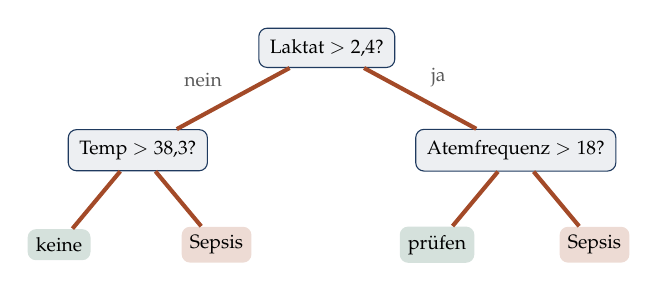
\begin{tikzpicture}[scale=1.0, every node/.style={font=\scriptsize}]
\node[draw=tief, rounded corners=3pt, fill=tief!8, inner sep=4pt] (w) at (0,2.4) {Laktat $> 2{,}4$?};
\node[draw=tief, rounded corners=3pt, fill=tief!8, inner sep=4pt] (a) at (-2.4,1.1) {Temp $> 38{,}3$?};
\node[draw=tief, rounded corners=3pt, fill=tief!8, inner sep=4pt] (b) at (2.4,1.1) {Atemfrequenz $> 18$?};
\node[fill=gruen!20, rounded corners=3pt, inner sep=3pt] (a1) at (-3.4,-0.1) {keine};
\node[fill=akzent!20, rounded corners=3pt, inner sep=3pt] (a2) at (-1.4,-0.1) {Sepsis};
\node[fill=gruen!20, rounded corners=3pt, inner sep=3pt] (b1) at (1.4,-0.1) {prüfen};
\node[fill=akzent!20, rounded corners=3pt, inner sep=3pt] (b2) at (3.4,-0.1) {Sepsis};
\draw[kanted] (w)--(a) node[midway,above left,color=grau] {nein};
\draw[kanted] (w)--(b) node[midway,above right,color=grau] {ja};
\draw[kanted] (a)--(a1); \draw[kanted] (a)--(a2);
\draw[kanted] (b)--(b1); \draw[kanted] (b)--(b2);
\end{tikzpicture}
\end{center}

\begin{center}
\begin{minipage}{0.9\textwidth}
\textbf{Ein Entscheidungsbaum --- die älteste Form klinischer Regeln, und zugleich ein Lernverfahren.}
\end{minipage}
\end{center}

\schritt{Die Daten}
$500$ Patienten, sieben Merkmale: Temperatur, Herzfrequenz, Laktat, Atemfrequenz, Alter --- und zwei reine Zufallszahlen, die mit nichts zusammenhängen.

\begin{center}
\begin{minipage}{0.88\textwidth}
\kursiv{Die Zufallszahlen sind absichtlich hinzugefügt. \textbf{In echten Daten weiß man nie, welche Merkmale nur Rauschen sind} --- und ein gutes Verfahren sollte sie ignorieren. Wir werden sehen, ob es das tut.}
\end{minipage}
\end{center}
\end{merksatz}

\section{Wie ein Baum wächst}

\begin{merksatz}
\boxtitel{Das Verfahren}
\begin{center}
{\small
\renewcommand{\arraystretch}{1.5}
\begin{tabular}{@{}P{1.0cm}P{7.4cm}@{}}
\toprule
$1$ & Suche unter allen Merkmalen und allen Schwellen die Frage, die die Patienten am besten in zwei \enquote{reine} Gruppen teilt.\\
$2$ & Wende dasselbe auf jede der beiden Gruppen an.\\
$3$ & Höre auf, wenn eine Gruppe rein ist oder zu klein wird.\\
\bottomrule
\end{tabular}}
\end{center}

\begin{center}
\begin{minipage}{0.88\textwidth}
\kursiv{Das Verfahren ist \Begriff{gierig}: Es wählt in jedem Schritt die beste Frage, ohne zu prüfen, ob eine schlechtere jetzt eine bessere später ermöglicht hätte. \textbf{Den global besten Baum zu finden, ist $\mathsf{NP}$-schwer} (Band 19, Kapitel~14) --- also begnügt man sich mit dem schrittweise besten.}
\end{minipage}
\end{center}
\end{merksatz}

\begin{definition}
\boxtitelm{Definition 9.1 --- Unreinheit}
Für eine Gruppe mit Sepsisanteil $p$:
\begin{center}
{\small
\renewcommand{\arraystretch}{1.55}
\begin{tabular}{@{}P{2.4cm}P{3.6cm}P{2.6cm}@{}}
\toprule
\textbf{Maß} & \textbf{Formel} & \textbf{Maximum bei}\\
\midrule
Entropie & $-p\log_2 p - (1-p)\log_2(1-p)$ & $p = \tfrac12$: $1$ bit\\
Gini & $2p\,(1-p)$ & $p = \tfrac12$: $\tfrac12$\\
\bottomrule
\end{tabular}}
\end{center}
Der \Begriff{Informationsgewinn} einer Frage ist die Unreinheit vorher minus der gewichtete Mittelwert der Unreinheiten danach.
\end{definition}

\begin{merksatz}
\boxtitel{Die Verbindung zu Band 20}
\begin{center}
\begin{minipage}{0.88\textwidth}
\kursiv{Die Entropie ist die aus Band 20, Kapitel~2; der Informationsgewinn ist die Transinformation zwischen Frage und Diagnose aus Kapitel~4 desselben Bandes. \textbf{Ein Entscheidungsbaum stellt diejenige Frage, deren Antwort am meisten über die Diagnose verrät} --- genau das tut ein guter Arzt, und genau das misst die Transinformation.}
\end{minipage}
\end{center}

\begin{center}
\begin{minipage}{0.88\textwidth}
\kursiv{Gini ist eine quadratische Näherung der Entropie und rechnet ohne Logarithmen. \textbf{In der Praxis wählen beide fast immer dieselbe Frage}, wie Aufgabe 9.1 zeigt.}
\end{minipage}
\end{center}
\end{merksatz}

\section{Der Leitfall gerechnet}

\begin{merksatz}
\boxtitel{Ein Baum der Tiefe drei}
Aus $500$ Patienten gelernt:
\begin{center}
{\small
\renewcommand{\arraystretch}{1.36}
\begin{tabular}{@{}P{8.4cm}@{}}
\toprule
\texttt{Laktat $\le$ 2,43}\\
\quad\texttt{Temp $\le$ 38,25}\ $\to$ \texttt{keine}\\
\quad\texttt{Temp $>$ 38,25}\\
\qquad\texttt{Laktat $\le$ 1,17}\ $\to$ \texttt{keine}\\
\qquad\texttt{Laktat $>$ 1,17}\ $\to$ \texttt{Sepsis}\\
\texttt{Laktat $>$ 2,43}\\
\quad\texttt{Atemfrequenz $>$ 17,8}\ $\to$ \texttt{Sepsis}\\
\quad\texttt{Atemfrequenz $\le$ 17,8}\\
\qquad\texttt{Temp $>$ 37,63}\ $\to$ \texttt{Sepsis}\\
\qquad\texttt{Temp $\le$ 37,63}\ $\to$ \texttt{keine}\\
\bottomrule
\end{tabular}}
\end{center}

\begin{center}
\begin{minipage}{0.9\textwidth}
\textbf{Die Wurzelfrage ist die Laktatschwelle von $2{,}43$ --- fast genau die Bayes-Schwelle aus Kapitel~1.}
\end{minipage}
\end{center}

\begin{center}
\begin{minipage}{0.88\textwidth}
\kursiv{Man kann den Baum lesen, prüfen und am Bett anwenden. \textbf{Er hat allerdings die Untertemperatur übersehen}: Im linken Ast fragt er nur nach Fieber. Bei Tiefe drei hat er nicht genug Fragen für beide Richtungen. Das zeigt die Grenze kleiner Bäume --- und den Grund, warum man sie größer werden lässt.}
\end{minipage}
\end{center}
\end{merksatz}

\begin{merksatz}
\boxtitel{Klein, groß, und viele}
Geprüft an $20\,000$ neuen Patienten:
\begin{center}
{\small
\renewcommand{\arraystretch}{1.48}
\begin{tabular}{@{}P{3.4cm}P{1.8cm}P{1.6cm}P{1.6cm}@{}}
\toprule
\textbf{Verfahren} & \textbf{Training} & \textbf{Test} & \textbf{Trennsch.}\\
\midrule
Baum, Tiefe 3 & $2{,}4\,\%$ & $3{,}5\,\%$ & $0{,}946$\\
Baum, voll ($13$ Blätter) & $0{,}0\,\%$ & $2{,}9\,\%$ & $0{,}952$\\
logistische Regression & $1{,}4\,\%$ & $2{,}8\,\%$ & $0{,}991$\\
\midrule
$200$ Bäume gemittelt & $0{,}0\,\%$ & $1{,}4\,\%$ & $0{,}998$\\
Zufallswald & $0{,}0\,\%$ & $\mathbf{1{,}2\,\%}$ & $\mathbf{0{,}999}$\\
Boosting & $0{,}0\,\%$ & $\mathbf{1{,}2\,\%}$ & $\mathbf{0{,}999}$\\
\bottomrule
\end{tabular}}
\end{center}

\begin{center}
\begin{minipage}{0.9\textwidth}
\textbf{Ein einzelner Baum ist so gut wie die logistische Regression. Zweihundert Bäume halbieren den Fehler.}
\end{minipage}
\end{center}

\begin{center}
\begin{minipage}{0.88\textwidth}
\kursiv{Die untere Hälfte der Tabelle ist das Thema dieses Kapitels. \textbf{Man verbessert ein Verfahren nicht, indem man es klüger macht, sondern indem man viele davon befragt} --- und zwar so, dass sie sich in ihren Fehlern möglichst unterscheiden.}
\end{minipage}
\end{center}
\end{merksatz}

\section{Warum ein Baum nicht reicht}

\begin{warnung}
\boxtitelr{Bäume sind instabil}
Man ziehe $200$-mal eine neue Stichprobe gleicher Größe (mit Zurücklegen) aus denselben $500$ Patienten und lerne jedes Mal einen Baum der Tiefe drei.

\begin{center}
{\small
\renewcommand{\arraystretch}{1.5}
\begin{tabular}{@{}P{3.4cm}P{5.2cm}@{}}
\toprule
\textbf{Wurzel} & $199$-mal Laktat, einmal Atemfrequenz\\
\textbf{Laktatschwelle} & zwischen $2{,}04$ und $2{,}67$ ($90\,\%$ der Fälle)\\
\textbf{rechter Ast, zweite Frage} & $142$-mal Atemfrequenz --- aber \textcolor{akzent}{$43$-mal eine Zufallszahl}\\
\bottomrule
\end{tabular}}
\end{center}

\begin{center}
\begin{minipage}{0.9\textwidth}
\textbf{In jedem fünften Baum steht an zweiter Stelle ein Merkmal, das mit nichts zusammenhängt.}
\end{minipage}
\end{center}

\begin{center}
\begin{minipage}{0.88\textwidth}
\kursiv{Die Wurzel ist stabil, weil das Laktat stark wirkt. \textbf{Weiter unten werden die Gruppen klein}, und in kleinen Gruppen kann eine Zufallszahl zufällig gut trennen --- genau das Problem aus Kapitel~3, Abschnitt über die höchste Zufallskorrelation. Und weil jede Frage die folgenden bestimmt, pflanzt sich ein zufälliger Fehler nach unten fort. Bäume haben kleine Verzerrung und große Varianz.}
\end{minipage}
\end{center}

\schritt{Die Folge für klinische Regeln}
\begin{center}
\begin{minipage}{0.88\textwidth}
\kursiv{\textbf{Ein aus Daten gelernter Entscheidungsbaum ist eine von vielen möglichen}, und wer ihn als Leitlinie veröffentlicht, veröffentlicht auch seine Zufälle. Die Wurzel verdient Vertrauen, die Blätter nur, wenn sie über viele Stichproben stabil sind.}
\end{minipage}
\end{center}
\end{warnung}

\section{Viele Bäume}

\begin{merksatz}
\boxtitel{Satz 9.2 --- die Varianz eines Mittelwerts}
Seien $Z_1,\ldots,Z_B$ Vorhersagen mit gleicher Varianz $\sigma^{2}$ und paarweiser Korrelation $\rho$. Dann gilt
\[ \operatorname{Var}\left[\frac1B\sum_{b=1}^{B}Z_b\right] = \rho\,\sigma^{2} + \frac{1-\rho}{B}\,\sigma^{2} . \]

\schritt{Beweis}
\[ \operatorname{Var}\left[\sum_b Z_b\right] = \sum_b\operatorname{Var}[Z_b] + \sum_{b\ne c}\operatorname{Cov}[Z_b,Z_c] = B\,\sigma^{2} + B(B-1)\,\rho\,\sigma^{2} \]
Division durch $B^{2}$:
\[ \frac{\sigma^{2}}{B} + \frac{(B-1)\rho\sigma^{2}}{B} = \rho\sigma^{2} + \frac{(1-\rho)\sigma^{2}}{B} \]
$\blacksquare$

\begin{center}
{\small
\renewcommand{\arraystretch}{1.5}
\begin{tabular}{@{}P{2.4cm}P{6.2cm}@{}}
\toprule
\textbf{Unabhängig, $\rho = 0$} & Varianz $\sigma^{2}/B$ --- beliebig klein.\\
\textbf{Gleich, $\rho = 1$} & Varianz $\sigma^{2}$ --- Mitteln nützt nichts.\\
\textbf{Dazwischen} & Mitteln drückt die Varianz auf $\rho\sigma^{2}$, nicht weiter.\\
\bottomrule
\end{tabular}}
\end{center}

\begin{center}
\begin{minipage}{0.9\textwidth}
\textbf{Mitteln hilft nur so weit, wie die Bäume sich unterscheiden.}
\end{minipage}
\end{center}
\end{merksatz}

\begin{merksatz}
\boxtitel{Zwei Wege zu unterschiedlichen Bäumen}
\begin{center}
{\small
\renewcommand{\arraystretch}{1.55}
\begin{tabular}{@{}P{2.4cm}P{6.2cm}@{}}
\toprule
\textbf{Bagging} & Jeder Baum lernt auf einer anderen Stichprobe mit Zurücklegen. Die Bäume unterscheiden sich, weil ihre Daten sich unterscheiden.\\
\textbf{Zufallswald} & Zusätzlich darf jeder Baum bei jeder Frage nur eine zufällige Auswahl der Merkmale betrachten. Die Bäume unterscheiden sich noch mehr.\\
\bottomrule
\end{tabular}}
\end{center}

\begin{center}
\begin{minipage}{0.88\textwidth}
\kursiv{Beim Bagging fragen fast alle Bäume zuerst nach dem Laktat --- sie sind sich ähnlich, $\rho$ bleibt groß. \textbf{Der Zufallswald verbietet einem Teil der Bäume das Laktat an der Wurzel}, und sie müssen mit Temperatur oder Atemfrequenz beginnen. Jeder einzelne wird dadurch schlechter, aber $\rho$ sinkt --- und nach Satz 9.2 kann das den Mittelwert verbessern.}
\end{minipage}
\end{center}

\begin{center}
\begin{minipage}{0.88\textwidth}
\kursiv{Das ist die Weisheit der vielen, mit einer Bedingung: \textbf{Sie gilt nur für eine Menge, die unabhängig urteilt.} Ein Gremium, in dem alle dieselben Unterlagen lesen und dieselbe Ausbildung hatten, ist nach Satz 9.2 kaum klüger als eines seiner Mitglieder.}
\end{minipage}
\end{center}
\end{merksatz}

\section{Aus Schwachen einen Starken machen}

\begin{merksatz}
\boxtitel{Die Idee des Boosting}
Man lernt die Bäume nicht unabhängig, sondern nacheinander --- und jeder neue achtet besonders auf die Patienten, bei denen die bisherigen falsch lagen.

\schritt{Das Verfahren AdaBoost}
Etiketten $t_i \in \{-1,+1\}$, Anfangsgewichte $D_1(i) = 1/n$.

\begin{center}
{\small
\renewcommand{\arraystretch}{1.5}
\begin{tabular}{@{}P{1.0cm}P{7.4cm}@{}}
\toprule
$1$ & Lerne eine einfache Regel $h_s$ auf den gewichteten Daten. Ihr gewichteter Fehler sei $\varepsilon_s < \tfrac12$.\\
$2$ & Gib ihr das Stimmgewicht $\alpha_s = \tfrac12\ln\frac{1-\varepsilon_s}{\varepsilon_s}$.\\
$3$ & Multipliziere die Gewichte falsch eingeordneter Patienten mit $e^{\alpha_s}$, richtig eingeordneter mit $e^{-\alpha_s}$, und normiere mit der Summe $Z_s$.\\
$4$ & Die Endregel ist $\operatorname{sign}\sum_s \alpha_s h_s(\vek x)$.\\
\bottomrule
\end{tabular}}
\end{center}
\end{merksatz}

\begin{merksatz}
\boxtitel{Satz 9.3 --- Freund und Schapire, 1995}
Der Trainingsfehler der Endregel nach $S$ Runden ist höchstens
\[ \prod_{s=1}^{S} Z_s = \prod_{s=1}^{S} 2\sqrt{\varepsilon_s(1-\varepsilon_s)} . \]

\schritt{Beweis}
Sei $F(\vek x) = \sum_s \alpha_s h_s(\vek x)$.

\kursiv{Erstens --- die Endgewichte:} Wendet man Schritt 3 $S$-mal an, so ist
\[ D_{S+1}(i) = \frac{e^{-t_i F(\vek x_i)}}{n\prod_s Z_s} , \]
denn jede Runde multipliziert mit $e^{-\alpha_s t_i h_s(\vek x_i)}$ und teilt durch $Z_s$. Da die $D_{S+1}(i)$ sich zu eins summieren:
\[ \frac1n\sum_i e^{-t_iF(\vek x_i)} = \prod_s Z_s . \]

\kursiv{Zweitens --- Fehler gegen Exponent:} Ist $\vek x_i$ falsch eingeordnet, so ist $t_iF(\vek x_i) \le 0$ und $e^{-t_iF} \ge 1$. Also
\[ \text{Trainingsfehler} = \frac1n\sum_i[t_iF(\vek x_i) \le 0] \ \le\ \frac1n\sum_i e^{-t_iF(\vek x_i)} = \prod_s Z_s . \]

\kursiv{Drittens --- $Z_s$ ausrechnen:} Falsche tragen zusammen das Gewicht $\varepsilon_s$, richtige $1-\varepsilon_s$:
\[ Z_s = \varepsilon_s e^{\alpha_s} + (1-\varepsilon_s)e^{-\alpha_s} = \varepsilon_s\sqrt{\tfrac{1-\varepsilon_s}{\varepsilon_s}} + (1-\varepsilon_s)\sqrt{\tfrac{\varepsilon_s}{1-\varepsilon_s}} = 2\sqrt{\varepsilon_s(1-\varepsilon_s)} \]
$\blacksquare$

\begin{center}
\begin{minipage}{0.9\textwidth}
\textbf{Ist jede Regel auch nur etwas besser als Raten, so fällt der Trainingsfehler exponentiell.}
\end{minipage}
\end{center}

\kursiv{Mit $\varepsilon_s = \tfrac12 - \gamma$:} $2\sqrt{(\tfrac12-\gamma)(\tfrac12+\gamma)} = \sqrt{1-4\gamma^{2}} \le e^{-2\gamma^{2}}$, also
\[ \text{Trainingsfehler} \ \le\ e^{-2\gamma^{2}S} . \]

\begin{center}
\begin{minipage}{0.88\textwidth}
\kursiv{\textbf{Aus schwachen Regeln wird eine beliebig starke} --- das war 1988 eine offene Frage von \Person{Michael Kearns} und \Person{Leslie Valiant}, und Boosting ist die Antwort. Dass der \kursiv{Testfehler} dabei nicht explodiert, obwohl der Trainingsfehler null wird, ist ein eigenes Rätsel; seine Lösung führt über den Rand aus Kapitel~8.}
\end{minipage}
\end{center}
\end{merksatz}

\section{Der Bruchfall}

\begin{warnung}
\boxtitelr{Was der Wald kostet}
\begin{center}
{\small
\renewcommand{\arraystretch}{1.52}
\begin{tabular}{@{}P{3.2cm}P{5.4cm}@{}}
\toprule
\textbf{Deutbarkeit} & Ein Baum lässt sich lesen. Zweihundert nicht.\\
\textbf{Außerhalb} & Bäume sagen jenseits der Trainingsdaten den Wert des äußersten Blattes vorher --- konstant, gleich wie weit man sich entfernt.\\
\textbf{Wahrschein\-lichkeiten} & Anteile von Bäumen sind keine gut kalibrierten Wahrscheinlichkeiten.\\
\textbf{Wichtigkeit} & Die übliche Rangliste der Merkmale bevorzugt solche mit vielen möglichen Schwellen.\\
\bottomrule
\end{tabular}}
\end{center}

\schritt{Zur zweiten Zeile}
\begin{center}
\begin{minipage}{0.88\textwidth}
\kursiv{Hat kein Trainingspatient ein Laktat über $8$, so behandelt der Wald einen Patienten mit $15$ genau wie einen mit $8$. \textbf{Das ist harmlos, wenn die Wirkung dort flach wird, und gefährlich, wenn sie weiter steigt.} Anders als das Polynom aus Kapitel~2 schwingt ein Baum außerhalb nicht aus --- aber er bleibt auch stehen, wo er weitergehen sollte.}
\end{minipage}
\end{center}

\schritt{Zur vierten Zeile}
\begin{center}
\begin{minipage}{0.88\textwidth}
\kursiv{Ein stetiger Laborwert bietet Hunderte von Schwellen, ein Ja-Nein-Merkmal nur eine. \textbf{Das stetige wird öfter gewählt und erscheint wichtiger} --- auch wenn es reines Rauschen ist. Man muss die Wichtigkeit durch zufälliges Vertauschen jedes Merkmals auf Testdaten messen, nicht aus dem Aufbau der Bäume ablesen.}
\end{minipage}
\end{center}
\end{warnung}

\section{Übungsaufgaben}

\begin{aufgabe}
\boxtitel{Aufgabe 9.1 --- Welche Frage zuerst?}
Von $100$ Patienten haben $20$ eine Sepsis. Zwei mögliche Fragen:
\begin{center}
{\small
\renewcommand{\arraystretch}{1.5}
\begin{tabular}{@{}P{2.6cm}P{2.6cm}P{2.6cm}@{}}
\toprule
\textbf{Frage} & \textbf{nein} & \textbf{ja}\\
\midrule
Laktat $> 2{,}4$ & $75$, davon $5$ Sepsis & $25$, davon $15$\\
Temperatur auffällig & $70$, davon $6$ & $30$, davon $14$\\
\bottomrule
\end{tabular}}
\end{center}
Berechnen Sie Informationsgewinn und Gini-Abnahme.

\loesung
\schritt{Schritt 1 --- Vorher}
\[ H(0{,}2) = -0{,}2\log_2 0{,}2 - 0{,}8\log_2 0{,}8 = 0{,}4644 + 0{,}2575 = 0{,}7219 \ \text{bit} \]
\[ G(0{,}2) = 2\cdot0{,}2\cdot0{,}8 = 0{,}32 \]

\schritt{Schritt 2 --- Laktat}
\begin{center}
{\small
\renewcommand{\arraystretch}{1.48}
\begin{tabular}{@{}P{1.6cm}P{1.4cm}P{1.6cm}P{1.8cm}P{1.6cm}@{}}
\toprule
\textbf{Gruppe} & \textbf{Anteil} & $p$ & $H$ & $G$\\
\midrule
nein & $0{,}75$ & $0{,}067$ & $0{,}3534$ & $0{,}1244$\\
ja & $0{,}25$ & $0{,}600$ & $0{,}9710$ & $0{,}4800$\\
\bottomrule
\end{tabular}}
\end{center}
\[ \text{nachher: } H = 0{,}75\cdot0{,}3534 + 0{,}25\cdot0{,}9710 = 0{,}2650+0{,}2428 = 0{,}5078 \]
\[ \text{Gewinn} = 0{,}7219 - 0{,}5078 = \mathbf{0{,}2142} \ \text{bit} \]
\[ G: \ 0{,}32 - (0{,}75\cdot0{,}1244 + 0{,}25\cdot0{,}48) = 0{,}32 - 0{,}2133 = \mathbf{0{,}1067} \]

\schritt{Schritt 3 --- Temperatur}
\begin{center}
{\small
\renewcommand{\arraystretch}{1.48}
\begin{tabular}{@{}P{1.6cm}P{1.4cm}P{1.6cm}P{1.8cm}P{1.6cm}@{}}
\toprule
\textbf{Gruppe} & \textbf{Anteil} & $p$ & $H$ & $G$\\
\midrule
nein & $0{,}70$ & $0{,}086$ & $0{,}4220$ & $0{,}1567$\\
ja & $0{,}30$ & $0{,}467$ & $0{,}9968$ & $0{,}4978$\\
\bottomrule
\end{tabular}}
\end{center}
\[ \text{Gewinn} = 0{,}7219 - (0{,}2954 + 0{,}2990) = \mathbf{0{,}1275} \ \text{bit} \]
\[ G: \ 0{,}32 - (0{,}1097 + 0{,}1493) = \mathbf{0{,}0610} \]

\schritt{Schritt 4 --- Die Entscheidung}
\begin{center}
{\small
\renewcommand{\arraystretch}{1.5}
\begin{tabular}{@{}P{2.8cm}P{2.2cm}P{2.2cm}@{}}
\toprule
& \textbf{Entropie} & \textbf{Gini}\\
\midrule
Laktat & $\mathbf{0{,}214}$ & $\mathbf{0{,}107}$\\
Temperatur & $0{,}128$ & $0{,}061$\\
\bottomrule
\end{tabular}}
\end{center}

\begin{center}
\begin{minipage}{0.88\textwidth}
\kursiv{\textbf{Beide Maße wählen das Laktat.} Die Antwort auf die Laktatfrage verrät $0{,}21$ bit über die Diagnose --- knapp ein Drittel der gesamten Unsicherheit von $0{,}72$ bit. Die Temperaturfrage verrät weniger, weil ihre \enquote{Ja}-Gruppe mit $47$ Prozent Sepsis kaum reiner ist als ein Münzwurf.}
\end{minipage}
\end{center}
\end{aufgabe}

\begin{aufgabe}
\boxtitel{Aufgabe 9.2 --- Wie viele Bäume?}
Einzelne Bäume haben an einem Punkt die Vorhersagevarianz $\sigma^{2} = 0{,}04$ und untereinander die Korrelation $\rho$. Berechnen Sie die Varianz des Mittels.

\loesung
\schritt{Schritt 1 --- Die Formel aus Satz 9.2}
\[ V(B,\rho) = \rho\cdot0{,}04 + \frac{(1-\rho)\cdot0{,}04}{B} \]

\schritt{Schritt 2 --- Die Werte}
\begin{center}
{\small
\renewcommand{\arraystretch}{1.48}
\begin{tabular}{@{}P{1.4cm}P{1.8cm}P{1.8cm}P{1.8cm}@{}}
\toprule
$B$ & $\rho = 0{,}8$ & $\rho = 0{,}5$ & $\rho = 0{,}2$\\
\midrule
$1$ & $0{,}0400$ & $0{,}0400$ & $0{,}0400$\\
$10$ & $0{,}0328$ & $0{,}0220$ & $0{,}0112$\\
$100$ & $0{,}0321$ & $0{,}0202$ & $0{,}0083$\\
$\infty$ & $0{,}0320$ & $0{,}0200$ & $0{,}0080$\\
\bottomrule
\end{tabular}}
\end{center}

\kursiv{Beispiel $B = 10$, $\rho = 0{,}5$:} $0{,}5\cdot0{,}04 + \frac{0{,}5\cdot0{,}04}{10} = 0{,}020 + 0{,}002 = 0{,}022$.

\schritt{Schritt 3 --- Zwei Lehren}
\begin{center}
{\small
\renewcommand{\arraystretch}{1.5}
\begin{tabular}{@{}P{2.4cm}P{6.2cm}@{}}
\toprule
\textbf{Die Zahl} & Ab etwa $B = 10$ bringen weitere Bäume kaum etwas.\\
\textbf{Die Korrelation} & Von $\rho = 0{,}8$ auf $0{,}2$ zu kommen, viertelt die Varianz --- mehr als jede Zahl von Bäumen.\\
\bottomrule
\end{tabular}}
\end{center}

\begin{center}
\begin{minipage}{0.88\textwidth}
\kursiv{\textbf{Darum lohnt der zusätzliche Zufall im Zufallswald}: Er verschlechtert jeden einzelnen Baum etwas, senkt aber die Korrelation deutlich. Und darum schadet eine große Zahl von Bäumen nie --- sie hilft nur ab einem gewissen Punkt nicht mehr. Überanpassung durch zu viele Bäume gibt es beim Mitteln nicht.}
\end{minipage}
\end{center}
\end{aufgabe}

\begin{aufgabe}
\boxtitel{Aufgabe 9.3 --- Eine Runde Boosting}
Zehn Patienten mit gleichem Gewicht $0{,}1$. Eine einfache Regel ordnet drei davon falsch ein. Führen Sie eine Runde AdaBoost aus.

\loesung
\schritt{Schritt 1 --- Fehler und Stimmgewicht}
\[ \varepsilon = 3\cdot0{,}1 = 0{,}3 \]
\[ \alpha = \tfrac12\ln\frac{0{,}7}{0{,}3} = \tfrac12\ln2{,}333 = \tfrac12\cdot0{,}8473 = 0{,}4236 \]

\schritt{Schritt 2 --- Die neuen Gewichte vor Normierung}
\[ e^{\alpha} = 1{,}5275, \qquad e^{-\alpha} = 0{,}6547 \]
\begin{center}
{\small
\renewcommand{\arraystretch}{1.48}
\begin{tabular}{@{}P{2.2cm}P{1.4cm}P{2.4cm}P{2.0cm}@{}}
\toprule
\textbf{Gruppe} & \textbf{Anzahl} & \textbf{neu je Patient} & \textbf{zusammen}\\
\midrule
falsch & $3$ & $0{,}15275$ & $0{,}45825$\\
richtig & $7$ & $0{,}06547$ & $0{,}45829$\\
\midrule
$Z$ & & & $0{,}9165$\\
\bottomrule
\end{tabular}}
\end{center}

\kursiv{Probe:} $2\sqrt{0{,}3\cdot0{,}7} = 2\sqrt{0{,}21} = 2\cdot0{,}4583 = 0{,}9165$ \checkmark

\schritt{Schritt 3 --- Nach Normierung}
\begin{center}
{\small
\renewcommand{\arraystretch}{1.48}
\begin{tabular}{@{}P{2.2cm}P{2.4cm}P{2.4cm}@{}}
\toprule
\textbf{Gruppe} & \textbf{je Patient} & \textbf{zusammen}\\
\midrule
falsch & $0{,}1667$ & $\mathbf{0{,}500}$\\
richtig & $0{,}0714$ & $\mathbf{0{,}500}$\\
\bottomrule
\end{tabular}}
\end{center}

\begin{center}
\begin{minipage}{0.9\textwidth}
\textbf{Nach der Neugewichtung tragen die falsch Eingeordneten genau die Hälfte des Gewichts.}
\end{minipage}
\end{center}

\schritt{Schritt 4 --- Warum das kein Zufall ist}
\kursiv{Falsche:} $\frac{\varepsilon\,e^{\alpha}}{Z} = \frac{\varepsilon\sqrt{(1-\varepsilon)/\varepsilon}}{2\sqrt{\varepsilon(1-\varepsilon)}} = \frac{\sqrt{\varepsilon(1-\varepsilon)}}{2\sqrt{\varepsilon(1-\varepsilon)}} = \frac12$

\begin{center}
\begin{minipage}{0.88\textwidth}
\kursiv{\textbf{Die alte Regel ist auf den neuen Gewichten genau so gut wie Raten.} Die nächste Regel muss also etwas anderes finden als die vorige --- das Verfahren zwingt jede Runde, eine neue Sicht auf die Daten zu gewinnen. Es ist das Gegenstück zum Zufallswald: Dort entsteht die Verschiedenheit durch Zufall, hier durch Absicht.}
\end{minipage}
\end{center}

\schritt{Schritt 5 --- Wie schnell der Trainingsfehler fällt}
Wenn jede Runde $\varepsilon = 0{,}3$ erreicht:
\begin{center}
{\small
\renewcommand{\arraystretch}{1.46}
\begin{tabular}{@{}P{1.6cm}P{2.4cm}P{2.4cm}@{}}
\toprule
\textbf{Runden} & $0{,}9165^{S}$ & $e^{-0{,}08S}$\\
\midrule
$10$ & $0{,}418$ & $0{,}449$\\
$20$ & $0{,}175$ & $0{,}202$\\
$50$ & $0{,}013$ & $0{,}018$\\
\bottomrule
\end{tabular}}
\end{center}

\kursiv{Zur rechten Spalte:} $\gamma = 0{,}5-0{,}3 = 0{,}2$, $2\gamma^{2} = 0{,}08$.
\end{aufgabe}

\begin{geschichte}
\boxtitelg{Zwei Lager, ein Verfahren}
\Person{Leo Breiman} (1928--2005) veröffentlichte 1984 mit \Person{Jerome Friedman}, \Person{Richard Olshen} und \Person{Charles Stone} das Buch über Klassifikations- und Regressionsbäume.

\begin{center}
\begin{minipage}{0.9\textwidth}
\kursiv{Etwa gleichzeitig entwickelte \Person{Ross Quinlan} in Australien die Entscheidungsbaumverfahren ID3 und C4.5 aus der Sicht der künstlichen Intelligenz. \textbf{Die beiden Gruppen arbeiteten lange nebeneinander, ohne einander zu zitieren} --- Statistiker und Informatiker hatten verschiedene Zeitschriften, Tagungen und Begriffe. Quinlan benutzte die Entropie, Breiman das Gini-Maß.}
\end{minipage}
\end{center}

\schritt{Bagging und Zufallswälder}
Breiman schlug 1996 das Bagging vor und 2001 den Zufallswald.

\begin{center}
\begin{minipage}{0.9\textwidth}
\kursiv{Im selben Jahr veröffentlichte er einen Aufsatz über die \enquote{zwei Kulturen} der Statistik: die eine, die Daten durch ein angenommenes Modell erklärt, und die andere, die nur Vorhersagegüte misst. \textbf{Er warf der Statistik vor, sich zu sehr an die erste zu klammern.} Der Aufsatz löste heftigen Widerspruch aus und gilt heute als Wendepunkt.}
\end{minipage}
\end{center}

\schritt{Boosting}
\begin{center}
\begin{minipage}{0.9\textwidth}
\kursiv{\Person{Robert Schapire} bewies 1990, dass schwache Lernbarkeit starke nach sich zieht; mit \Person{Yoav Freund} gab er 1995 AdaBoost an. \textbf{Beide erhielten 2003 den Gödel-Preis} --- einen Preis für theoretische Informatik, für ein Verfahren, das zugleich zu den praktisch erfolgreichsten gehört.}
\end{minipage}
\end{center}
\end{geschichte}

\begin{forschung}
\boxtitelp{Wälder heute}
\begin{center}
{\small
\renewcommand{\arraystretch}{1.45}
\begin{tabular}{@{}P{2.8cm}P{5.4cm}@{}}
\toprule
\textbf{Tabellarische Daten} & Gradient-Boosting schlägt tiefe Netze bei Tabellen --- bis heute meist.\\
\textbf{Ursachen schätzen} & Wälder, die Behandlungseffekte je Patient schätzen.\\
\textbf{Erklären} & Shapley-Werte aus Band 21 für die Beiträge einzelner Merkmale.\\
\bottomrule
\end{tabular}}
\end{center}

\schritt{Zur dritten Zeile}
\begin{center}
\begin{minipage}{0.88\textwidth}
\kursiv{Um zu erklären, warum der Wald bei einem bestimmten Patienten warnt, behandelt man die Merkmale als Spieler eines kooperativen Spiels und verteilt die Vorhersage nach dem Shapley-Wert aus Band 21, Kapitel~14. \textbf{Die dort beschriebenen Vorbehalte gelten hier genauso}: Verbundene Merkmale teilen sich die Anerkennung auf eine Weise, die von der gewählten Behandlung fehlender Merkmale abhängt, und die Erklärung beschreibt das Modell, nicht die Krankheit.}
\end{minipage}
\end{center}
\end{forschung}

\begin{merksatz}
\boxtitel{Was Sie jetzt können}
\begin{center}
\renewcommand{\arraystretch}{1.5}
\begin{tabular}{@{}P{3.0cm}P{5.6cm}@{}}
\toprule
\textbf{Definition 9.1} & Entropie, Gini, Informationsgewinn\\
\textbf{Instabilität} & kleine Verzerrung, große Varianz\\
\textbf{Satz 9.2} & Mittel: $\rho\sigma^{2} + (1-\rho)\sigma^{2}/B$\\
\textbf{Satz 9.3} & Boosting: Fehler $\le \prod 2\sqrt{\varepsilon_s(1-\varepsilon_s)}$\\
\textbf{Der Bruchfall} & deutbar nur einzeln\\
\bottomrule
\end{tabular}
\end{center}

\begin{center}
\begin{minipage}{0.88\textwidth}
\kursiv{Bäume fragen nach Schwellen. Das nächste Kapitel fragt nach Nachbarn --- und stößt auf ein Problem, das in hohen Dimensionen alle Verfahren trifft.}
\end{minipage}
\end{center}
\end{merksatz}

\chapter{Ähnliche Fälle und der Fluch der Dimension}

\section{Der Leitfall}

\begin{merksatz}
\boxtitel{\enquote{Ich hatte mal einen Patienten wie diesen}}
Die erfahrene Oberärztin sieht den neuen Patienten an und erinnert sich an frühere mit ähnlichem Laktat und ähnlicher Herzfrequenz. Die meisten davon hatten eine Sepsis.

\begin{center}
\begin{minipage}{0.9\textwidth}
\textbf{Das ist ein Lernverfahren --- das einfachste, das es gibt, und eines der ältesten.}
\end{minipage}
\end{center}

\begin{center}
\begin{minipage}{0.88\textwidth}
\kursiv{Es braucht kein Modell, keine Parameter, keine Annahme über die Form der Grenze. \textbf{Es speichert alle Fälle und fragt im Bedarfsfall die ähnlichsten.} Man nennt das die Methode der nächsten Nachbarn --- und dieses Kapitel zeigt, dass sie in wenigen Dimensionen erstaunlich gut und in vielen erstaunlich schlecht ist.}
\end{minipage}
\end{center}
\end{merksatz}

\begin{definition}
\boxtitelm{Definition 10.1 --- $k$ nächste Nachbarn}
Für einen neuen Punkt $\vek x$:
\begin{center}
{\small
\renewcommand{\arraystretch}{1.5}
\begin{tabular}{@{}P{1.0cm}P{7.4cm}@{}}
\toprule
$1$ & Berechne den Abstand zu allen $n$ Trainingspunkten.\\
$2$ & Wähle die $k$ nächsten.\\
$3$ & Sage vorher, was die Mehrheit von ihnen hat --- oder den Anteil als Wahrscheinlichkeit.\\
\bottomrule
\end{tabular}}
\end{center}
\end{definition}

\begin{merksatz}
\boxtitel{Die Wahl von $k$}
$500$ Patienten mit Laktat und Herzfrequenz, beide auf gleiche Streuung gebracht:

\begin{center}
{\small
\renewcommand{\arraystretch}{1.46}
\begin{tabular}{@{}P{1.6cm}P{2.2cm}P{2.2cm}P{2.2cm}@{}}
\toprule
$k$ & \textbf{Training} & \textbf{Test} & \\
\midrule
$1$ & $0{,}0\,\%$ & $7{,}3\,\%$ & auswendig\\
$5$ & $3{,}2\,\%$ & $5{,}6\,\%$ & \\
$15$ & $3{,}8\,\%$ & $\mathbf{4{,}7\,\%}$ & \\
$51$ & $4{,}6\,\%$ & $4{,}9\,\%$ & \\
$151$ & $7{,}8\,\%$ & $7{,}5\,\%$ & \\
$401$ & $23{,}8\,\%$ & $20{,}4\,\%$ & alles gleich\\
\bottomrule
\end{tabular}}
\end{center}

\begin{center}
\begin{minipage}{0.9\textwidth}
\textbf{Die Kurve aus Kapitel~2 in neuer Gestalt: $k$ klein heißt Varianz, $k$ groß heißt Verzerrung.}
\end{minipage}
\end{center}

\begin{center}
\begin{minipage}{0.88\textwidth}
\kursiv{Bei $k = 1$ entscheidet ein einziger früherer Patient --- und wenn er ein Ausnahmefall war, überträgt sich die Ausnahme. Bei $k = 401$ fragt man fast alle, und da achtzig Prozent keine Sepsis hatten, sagt man fast immer \enquote{keine}. \textbf{Die Zahl $k$ ist die Stellgröße der Komplexität}, und man wählt sie durch Kreuzvalidierung wie den Grad des Polynoms.}
\end{minipage}
\end{center}
\end{merksatz}

\section{Wie gut kann das sein?}

\begin{merksatz}
\boxtitel{Satz 10.2 --- Cover und Hart, 1967}
Mit wachsender Datenmenge nähert sich der Fehler des Verfahrens mit einem einzigen Nachbarn einem Wert, der höchstens
\[ 2\,\Risk^{*}(1-\Risk^{*}) \ \le\ 2\,\Risk^{*} \]
beträgt --- dem Doppelten des Bayes-Risikos aus Kapitel~1.

\schritt{Der Gedanke}
Bei sehr vielen Daten liegt der nächste Nachbar beliebig nahe am neuen Punkt. Sein Etikett ist dann eine unabhängige Ziehung aus derselben Verteilung $\eta(\vek x)$.

\begin{center}
\begin{minipage}{0.86\textwidth}
\kursiv{Dass man bei hinreichend glattem $\eta$ so argumentieren darf, verlangt eine Grenzwertbetrachtung, die wir übergehen --- die sechste Auslassung dieses Bandes. \textbf{Der Rest des Beweises ist elementar.}}
\end{minipage}
\end{center}

\schritt{Beweis unter dieser Annahme}
\kursiv{An einer Stelle $\vek x$} haben neuer Punkt und Nachbar unabhängig mit Wahrscheinlichkeit $\eta$ Sepsis. Ein Fehler entsteht, wenn sie sich unterscheiden:
\[ \Pr[\text{Fehler} \mid \vek x] = \eta(1-\eta) + (1-\eta)\eta = 2\,\eta(1-\eta) . \]

\kursiv{Mit $m = \min\{\eta, 1-\eta\}$} ist $\eta(1-\eta) = m(1-m)$, und nach Satz 1.4 ist $\Risk^{*} = \E[m]$.

\kursiv{Mittelung über $\vek x$:}
\[ \Pr[\text{Fehler}] = 2\,\E[m(1-m)] = 2\bigl(\E[m] - \E[m^{2}]\bigr) \]

\kursiv{Da} $\E[m^{2}] \ge (\E[m])^{2}$ --- die Varianz ist nichtnegativ ---:
\[ \Pr[\text{Fehler}] \ \le\ 2\bigl(\Risk^{*} - (\Risk^{*})^{2}\bigr) = 2\,\Risk^{*}(1-\Risk^{*}) \]
$\blacksquare$

\begin{center}
\begin{minipage}{0.9\textwidth}
\textbf{Die Hälfte der verfügbaren Information steckt im nächsten Nachbarn.}
\end{minipage}
\end{center}

\begin{center}
\begin{minipage}{0.88\textwidth}
\kursiv{So haben Cover und Hart es selbst formuliert. \textbf{Ein Verfahren ohne jede Theorie, ohne Modell und ohne Parameter kommt bis auf den Faktor zwei an das Beste heran, was überhaupt möglich ist} --- vorausgesetzt, man hat genug Daten. Mit wachsendem $k$ und $k/n \to 0$ erreicht man sogar $\Risk^{*}$ selbst.}
\end{minipage}
\end{center}
\end{merksatz}

\section{Der Fluch der Dimension}

\begin{warnung}
\boxtitelr{Was mit Rauschmerkmalen geschieht}
Man füge den beiden sinnvollen Merkmalen $m$ weitere hinzu, die reines Rauschen sind. Immer $k = 15$, immer $500$ Patienten.

\begin{center}
{\small
\renewcommand{\arraystretch}{1.46}
\begin{tabular}{@{}P{2.8cm}P{2.4cm}@{}}
\toprule
\textbf{Rauschmerkmale} & \textbf{Testfehler}\\
\midrule
$0$ & $4{,}1\,\%$\\
$2$ & $5{,}8\,\%$\\
$5$ & $7{,}0\,\%$\\
$10$ & $9{,}5\,\%$\\
$20$ & $11{,}2\,\%$\\
$50$ & $14{,}9\,\%$\\
$100$ & $\mathbf{18{,}7\,\%}$\\
\midrule
nie warnen & $20{,}0\,\%$\\
\bottomrule
\end{tabular}}
\end{center}

\begin{center}
\begin{minipage}{0.9\textwidth}
\textbf{Mit hundert Rauschmerkmalen ist das Verfahren kaum besser als gar keines.}
\end{minipage}
\end{center}

\begin{center}
\begin{minipage}{0.88\textwidth}
\kursiv{\textbf{Das Verfahren kann nicht wissen, welche Merkmale zählen} --- es misst den Abstand über alle gleichermaßen. Hundert Rauschmerkmale tragen hundertmal so viel zum Abstand bei wie zwei sinnvolle, und die \enquote{nächsten} Nachbarn sind dann diejenigen, deren Rauschen zufällig ähnlich ist. Die logistische Regression aus Kapitel~5 würde den Rauschmerkmalen Koeffizienten nahe null geben und kaum leiden.}
\end{minipage}
\end{center}
\end{warnung}

\begin{merksatz}
\boxtitel{Drei Seiten desselben Problems}
\schritt{Erstens: Nachbarschaft wird groß}
Im Einheitswürfel mit $p$ Dimensionen will man einen Teilwürfel, der den Anteil $r$ der gleichverteilten Daten enthält. Seine Kantenlänge ist
\[ e = r^{1/p} . \]

\begin{center}
{\small
\renewcommand{\arraystretch}{1.46}
\begin{tabular}{@{}P{1.6cm}P{2.6cm}P{2.6cm}@{}}
\toprule
$p$ & $r = 1\,\%$ & $r = 10\,\%$\\
\midrule
$1$ & $0{,}01$ & $0{,}10$\\
$2$ & $0{,}10$ & $0{,}32$\\
$10$ & $0{,}63$ & $0{,}79$\\
$100$ & $0{,}95$ & $0{,}98$\\
\bottomrule
\end{tabular}}
\end{center}

\begin{center}
\begin{minipage}{0.88\textwidth}
\kursiv{\textbf{In zehn Dimensionen muss man zwei Drittel jeder Achse überspannen, um ein Prozent der Daten zu erfassen.} Die \enquote{Nachbarschaft} ist dann nicht mehr lokal --- sie umfasst Patienten mit ganz anderen Werten.}
\end{minipage}
\end{center}

\schritt{Zweitens: Abstände gleichen sich an}
$1000$ gleichverteilte Punkte, ein Suchpunkt:
\begin{center}
{\small
\renewcommand{\arraystretch}{1.46}
\begin{tabular}{@{}P{1.6cm}P{4.4cm}@{}}
\toprule
$p$ & $\dfrac{\text{größter} - \text{kleinster Abstand}}{\text{kleinster Abstand}}$\\
\midrule
$1$ & $1241$\\
$2$ & $45$\\
$10$ & $3{,}0$\\
$100$ & $0{,}46$\\
$1000$ & $0{,}13$\\
\bottomrule
\end{tabular}}
\end{center}

\begin{center}
\begin{minipage}{0.88\textwidth}
\kursiv{\textbf{In tausend Dimensionen ist der fernste Punkt nur dreizehn Prozent weiter weg als der nächste.} \enquote{Nächster Nachbar} bedeutet dann kaum noch etwas --- alle sind fast gleich weit entfernt.}
\end{minipage}
\end{center}

\schritt{Drittens: Alles liegt am Rand}
Der Anteil des Würfels, der näher als $0{,}05$ an einer Seite liegt:
\[ 1 - 0{,}9^{p} \]
\begin{center}
{\small
\renewcommand{\arraystretch}{1.46}
\begin{tabular}{@{}P{1.6cm}P{2.4cm}@{}}
\toprule
$p$ & \textbf{am Rand}\\
\midrule
$1$ & $10\,\%$\\
$10$ & $65\,\%$\\
$50$ & $99{,}5\,\%$\\
\bottomrule
\end{tabular}}
\end{center}

\begin{center}
\begin{minipage}{0.88\textwidth}
\kursiv{In fünfzig Dimensionen gibt es praktisch kein Inneres. \textbf{Jeder neue Punkt liegt am Rand der Daten --- also dort, wo nach Kapitel~2 jede Vorhersage unsicher wird.} Hohe Dimension heißt fast immer Extrapolation.}
\end{minipage}
\end{center}
\end{merksatz}

\begin{merksatz}
\boxtitel{Warum Lernen dennoch gelingt}
\begin{center}
{\small
\renewcommand{\arraystretch}{1.55}
\begin{tabular}{@{}P{2.6cm}P{6.0cm}@{}}
\toprule
\textbf{Wenige zählen} & Die meisten Merkmale sind unwichtig. Wer sie erkennt --- Lasso, Bäume ---, reduziert die wirksame Dimension.\\
\textbf{Daten sind nicht gleichverteilt} & Echte Daten liegen auf niedrigdimensionalen Flächen im hochdimensionalen Raum.\\
\textbf{Glattheit} & Ist der Zusammenhang glatt, genügen wenige Stützstellen.\\
\bottomrule
\end{tabular}}
\end{center}

\begin{center}
\begin{minipage}{0.88\textwidth}
\kursiv{Die zweite Zeile ist die wichtigste. Ein Röntgenbild hat eine Million Bildpunkte, aber die Menge möglicher Röntgenbilder von Brustkörben ist unvergleichlich kleiner als die Menge aller Bilder. \textbf{Die Daten füllen den Raum nicht} --- sie liegen auf einer dünnen Fläche darin, deren Dimension vielleicht einige Dutzend beträgt. Kapitel~13 behandelt, wie man diese Fläche findet.}
\end{minipage}
\end{center}
\end{merksatz}

\section{Der Bruchfall}

\begin{warnung}
\boxtitelr{Was \enquote{ähnlich} heißt}
\begin{center}
{\small
\renewcommand{\arraystretch}{1.52}
\begin{tabular}{@{}P{2.4cm}P{6.2cm}@{}}
\toprule
\textbf{Einheiten} & Ohne Normierung steigt der Fehler im Leitfall von $4{,}7$ auf $9{,}7$ Prozent --- die Herzfrequenz überdeckt das Laktat.\\
\textbf{Gewichtung} & Gleiche Streuung heißt nicht gleiche Wichtigkeit. Das Laktat verdient mehr Gewicht als das Alter.\\
\textbf{Art der Merkmale} & Wie weit ist \enquote{männlich} von \enquote{weiblich}? Wie weit Diagnose A von Diagnose B?\\
\bottomrule
\end{tabular}}
\end{center}

\begin{center}
\begin{minipage}{0.88\textwidth}
\kursiv{\textbf{Der Abstand ist das ganze Modell.} Beim Verfahren der nächsten Nachbarn steckt jede Annahme über die Aufgabe in der Wahl des Abstandsmaßes, und diese Wahl wird häufig nicht getroffen, sondern der euklidische Abstand stillschweigend übernommen.}
\end{minipage}
\end{center}

\schritt{Die Erfahrung der Oberärztin}
\begin{center}
\begin{minipage}{0.88\textwidth}
\kursiv{Die Oberärztin aus dem Leitfall wendet kein festes Abstandsmaß an. \textbf{Sie weiß, welche Merkmale bei welcher Frage zählen} --- beim Verdacht auf Sepsis das Laktat, bei Verdacht auf Lungenembolie andere Werte. Das ist eine gelernte, vom Zusammenhang abhängige Ähnlichkeit, und sie ist der Grund, warum menschliche Erfahrung trotz weniger Fälle so gut funktioniert. Verfahren, die solche Abstandsmaße lernen, sind ein eigenes Forschungsgebiet.}
\end{minipage}
\end{center}
\end{warnung}

\section{Übungsaufgaben}

\begin{aufgabe}
\boxtitel{Aufgabe 10.1 --- Nachbarn von Hand}
Sieben frühere Patienten (Laktat in mmol/l, Herzfrequenz in Zehnern pro Minute) und ein neuer, $Q = (2{,}2;\ 10{,}0)$:
\begin{center}
{\small
\renewcommand{\arraystretch}{1.44}
\begin{tabular}{@{}P{1.0cm}P{1.4cm}P{1.4cm}P{1.4cm}@{}}
\toprule
& \textbf{Laktat} & \textbf{HF} & \textbf{Sepsis}\\
\midrule
A & $1{,}0$ & $8{,}5$ & nein\\
B & $1{,}4$ & $9{,}0$ & nein\\
C & $2{,}8$ & $11{,}0$ & ja\\
D & $3{,}2$ & $10{,}5$ & ja\\
E & $2{,}0$ & $9{,}5$ & nein\\
F & $2{,}6$ & $9{,}8$ & ja\\
G & $1{,}8$ & $10{,}8$ & nein\\
\bottomrule
\end{tabular}}
\end{center}
Was sagt das Verfahren für $k = 1, 3, 5, 7$?

\loesung
\schritt{Schritt 1 --- Die Abstände}
\begin{center}
{\small
\renewcommand{\arraystretch}{1.46}
\begin{tabular}{@{}P{1.0cm}P{3.6cm}P{1.4cm}P{1.2cm}@{}}
\toprule
& \textbf{Rechnung} & \textbf{Abstand} & \textbf{Rang}\\
\midrule
F & $\sqrt{0{,}4^{2}+0{,}2^{2}} = \sqrt{0{,}20}$ & $0{,}447$ & $1$\\
E & $\sqrt{0{,}2^{2}+0{,}5^{2}} = \sqrt{0{,}29}$ & $0{,}539$ & $2$\\
G & $\sqrt{0{,}4^{2}+0{,}8^{2}} = \sqrt{0{,}80}$ & $0{,}894$ & $3$\\
D & $\sqrt{1{,}0^{2}+0{,}5^{2}} = \sqrt{1{,}25}$ & $1{,}118$ & $4$\\
C & $\sqrt{0{,}6^{2}+1{,}0^{2}} = \sqrt{1{,}36}$ & $1{,}166$ & $5$\\
B & $\sqrt{0{,}8^{2}+1{,}0^{2}} = \sqrt{1{,}64}$ & $1{,}281$ & $6$\\
A & $\sqrt{1{,}2^{2}+1{,}5^{2}} = \sqrt{3{,}69}$ & $1{,}921$ & $7$\\
\bottomrule
\end{tabular}}
\end{center}

\schritt{Schritt 2 --- Die Abstimmungen}
\begin{center}
{\small
\renewcommand{\arraystretch}{1.48}
\begin{tabular}{@{}P{1.2cm}P{2.6cm}P{1.4cm}P{1.4cm}P{1.6cm}@{}}
\toprule
$k$ & \textbf{Nachbarn} & \textbf{ja} & \textbf{nein} & \textbf{Urteil}\\
\midrule
$1$ & F & $1$ & $0$ & \textcolor{akzent}{Sepsis}\\
$3$ & F, E, G & $1$ & $2$ & \textcolor{gruen}{keine}\\
$5$ & $+$ D, C & $3$ & $2$ & \textcolor{akzent}{Sepsis}\\
$7$ & $+$ B, A & $3$ & $4$ & \textcolor{gruen}{keine}\\
\bottomrule
\end{tabular}}
\end{center}

\begin{center}
\begin{minipage}{0.9\textwidth}
\textbf{Das Urteil wechselt mit jedem $k$.}
\end{minipage}
\end{center}

\schritt{Schritt 3 --- Was das bedeutet}
\begin{center}
\begin{minipage}{0.88\textwidth}
\kursiv{Der neue Patient liegt genau im Grenzbereich --- die Anteile schwanken um die Hälfte: $1$, $\tfrac13$, $\tfrac35$, $\tfrac37$. \textbf{Das Verfahren sagt ehrlich, dass es unsicher ist}, wenn man es nach dem Anteil statt nach der Mehrheit fragt. Wer nur die Mehrheitsentscheidung weitergibt, versteckt diese Unsicherheit.}
\end{minipage}
\end{center}

\schritt{Schritt 4 --- Mit anderer Einheit}
\begin{center}
\begin{minipage}{0.88\textwidth}
\kursiv{Hätte man die Herzfrequenz in Schlägen statt in Zehnern angegeben, so wären die Unterschiede in der zweiten Spalte zehnmal größer, und das Laktat spielte praktisch keine Rolle mehr. Der nächste Nachbar wäre dann D oder F, je nach Herzfrequenz allein. \textbf{Die Wahl der Einheit ist hier eine Wahl des Modells.}}
\end{minipage}
\end{center}
\end{aufgabe}

\begin{aufgabe}
\boxtitel{Aufgabe 10.2 --- Die Schranke von Cover und Hart}
Berechnen Sie die asymptotische Fehlerschranke für einen Nachbarn bei verschiedenen Bayes-Risiken.

\loesung
\schritt{Schritt 1 --- Die Formel}
\[ 2\,\Risk^{*}(1-\Risk^{*}) \]

\schritt{Schritt 2 --- Die Werte}
\begin{center}
{\small
\renewcommand{\arraystretch}{1.48}
\begin{tabular}{@{}P{2.4cm}P{3.2cm}P{2.0cm}@{}}
\toprule
$\Risk^{*}$ & \textbf{Rechnung} & \textbf{Schranke}\\
\midrule
$1\,\%$ & $2\cdot0{,}01\cdot0{,}99$ & $1{,}98\,\%$\\
$3{,}47\,\%$ & $2\cdot0{,}0347\cdot0{,}9653$ & $6{,}70\,\%$\\
$10\,\%$ & $2\cdot0{,}1\cdot0{,}9$ & $18{,}0\,\%$\\
$30\,\%$ & $2\cdot0{,}3\cdot0{,}7$ & $42{,}0\,\%$\\
$50\,\%$ & $2\cdot0{,}5\cdot0{,}5$ & $50{,}0\,\%$\\
\bottomrule
\end{tabular}}
\end{center}

\kursiv{Die zweite Zeile ist das Laktat allein aus Kapitel~1.}

\schritt{Schritt 3 --- Die Lehre}
\begin{center}
{\small
\renewcommand{\arraystretch}{1.5}
\begin{tabular}{@{}P{2.4cm}P{6.2cm}@{}}
\toprule
\textbf{Leichte Aufgabe} & Die Schranke ist fast genau das Doppelte des Bestmöglichen.\\
\textbf{Unmögliche Aufgabe} & Bei $\Risk^{*} = \tfrac12$ kann niemand etwas --- und der Nachbar auch nicht.\\
\bottomrule
\end{tabular}}
\end{center}

\begin{center}
\begin{minipage}{0.88\textwidth}
\kursiv{\textbf{Der Faktor zwei ist der Preis dafür, nur einen einzigen Zeugen zu befragen.} Bei $k$ Nachbarn schrumpft er, und bei wachsendem $k$ mit $k/n \to 0$ verschwindet er ganz --- das zeigte \Person{Charles Stone} 1977. Man bezahlt dafür mit mehr Daten.}
\end{minipage}
\end{center}
\end{aufgabe}

\begin{aufgabe}
\boxtitel{Aufgabe 10.3 --- Wie viele Patienten in zehn Dimensionen?}
Bei $500$ gleichverteilten Patienten in zwei Dimensionen liegen die $15$ nächsten Nachbarn eines neuen Patienten in einem kleinen Quadrat. Wie viele Patienten braucht man in zehn Dimensionen, damit die $15$ Nachbarn in einem Würfel \kursiv{derselben Kantenlänge} liegen?

\loesung
\schritt{Schritt 1 --- Die Kantenlänge in zwei Dimensionen}
Die $15$ Nachbarn sind der Anteil $\frac{15}{500} = 0{,}03$ der Patienten. Ein Quadrat mit diesem Flächenanteil hat die Kante
\[ e = 0{,}03^{1/2} = 0{,}173 . \]

\schritt{Schritt 2 --- Dieselbe Kante in zehn Dimensionen}
Ein Würfel mit Kante $0{,}173$ umfasst dort den Anteil
\[ 0{,}173^{10} = 2{,}4\cdot10^{-8} . \]

\schritt{Schritt 3 --- Die nötige Datenmenge}
\[ n = \frac{15}{2{,}4\cdot10^{-8}} = 6{,}2\cdot10^{8} \]

\begin{center}
\begin{minipage}{0.9\textwidth}
\textbf{Sechshundert Millionen Patienten --- statt fünfhundert.}
\end{minipage}
\end{center}

\schritt{Schritt 4 --- Die allgemeine Regel}
\[ n_p = n_2\cdot\left(\frac{1}{e}\right)^{p-2} \]
\kursiv{Jede zusätzliche Dimension multipliziert den Bedarf mit $1/0{,}173 = 5{,}8$.}

\begin{center}
\begin{minipage}{0.88\textwidth}
\kursiv{\textbf{Das ist der Fluch der Dimension in einer Zahl.} Er trifft jedes Verfahren, das auf Nachbarschaft beruht, und damit mittelbar auch Bäume, Kerne und Netze. Dass sie trotzdem in hohen Dimensionen funktionieren, liegt nicht daran, dass sie den Fluch überwinden, sondern daran, dass echte Daten ihn nicht in voller Stärke auslösen --- weil sie, wie in Abschnitt 10.3 beschrieben, den Raum nicht füllen.}
\end{minipage}
\end{center}
\end{aufgabe}

\begin{geschichte}
\boxtitelg{Eine Luftwaffe, ein Bericht, ein Name}
\Person{Evelyn Fix} und \Person{Joseph Hodges} beschrieben das Verfahren der nächsten Nachbarn 1951 in einem Bericht für die Schule für Fliegermedizin der amerikanischen Luftwaffe.

\begin{center}
\begin{minipage}{0.9\textwidth}
\kursiv{Der Bericht blieb unveröffentlicht und wurde erst 1989 in einer Zeitschrift nachgedruckt. \textbf{Fix war eine der ersten Frauen, die in Berkeley in Statistik promoviert wurden}, und arbeitete ihr ganzes Berufsleben dort; ihr Beitrag zu einem der meistbenutzten Lernverfahren ist erst in den letzten Jahren angemessen gewürdigt worden.}
\end{minipage}
\end{center}

\schritt{Cover und Hart}
\Person{Thomas Cover} und \Person{Peter Hart} bewiesen 1967 den Satz dieses Kapitels.

\begin{center}
\begin{minipage}{0.9\textwidth}
\kursiv{Cover wurde später einer der führenden Informationstheoretiker --- sein Lehrbuch mit \Person{Joy Thomas} war eine der Hauptquellen von Band 20. \textbf{Hart entwickelte kurz darauf den A-Stern-Algorithmus für die kürzeste Wegsuche}, der heute in jedem Navigationsgerät steckt.}
\end{minipage}
\end{center}

\schritt{Bellman}
\Person{Richard Bellman} prägte 1957 den Ausdruck \enquote{Fluch der Dimension} --- in einem Buch über dynamische Programmierung.

\begin{center}
\begin{minipage}{0.9\textwidth}
\kursiv{Er meinte damit, dass eine Tabelle mit $10$ Stützstellen je Achse in $10$ Dimensionen $10^{10}$ Einträge hat. \textbf{Dass dasselbe Problem das Lernen beherrschen würde}, ahnte er, aber die Tragweite zeigte sich erst mit den hochdimensionalen Daten der Genomforschung und der Bildverarbeitung.}
\end{minipage}
\end{center}
\end{geschichte}

\begin{forschung}
\boxtitelp{Nachbarn heute}
\begin{center}
{\small
\renewcommand{\arraystretch}{1.45}
\begin{tabular}{@{}P{2.8cm}P{5.4cm}@{}}
\toprule
\textbf{Schnelle Suche} & Nächste Nachbarn unter Milliarden von Punkten in Millisekunden --- näherungsweise.\\
\textbf{Gelernte Abstände} & Netze, die Bilder oder Texte in Räume abbilden, in denen der euklidische Abstand Ähnlichkeit misst.\\
\textbf{Fallbasierte Medizin} & Ähnliche Patienten aus der Krankenakte finden.\\
\bottomrule
\end{tabular}}
\end{center}

\schritt{Zur zweiten Zeile}
\begin{center}
\begin{minipage}{0.88\textwidth}
\kursiv{Moderne Sprachmodelle arbeiten intern mit Vektoren von einigen tausend Dimensionen. \textbf{Das Suchen ähnlicher Texte ist dort ein Suchen nächster Nachbarn} --- und funktioniert trotz der Dimension, weil die Abbildung gelernt wurde, um genau diese Ähnlichkeit zu erhalten. Der Fluch ist nicht überwunden, sondern umgangen: Man lernt zuerst den Raum, in dem Nachbarschaft Sinn ergibt, und sucht dann darin.}
\end{minipage}
\end{center}
\end{forschung}

\begin{merksatz}
\boxtitel{Was Sie jetzt können}
\begin{center}
\renewcommand{\arraystretch}{1.5}
\begin{tabular}{@{}P{3.0cm}P{5.6cm}@{}}
\toprule
\textbf{Definition 10.1} & $k$ Nachbarn, Mehrheit oder Anteil\\
\textbf{Satz 10.2} & ein Nachbar: höchstens $2\Risk^{*}(1-\Risk^{*})$\\
\textbf{Kantenlänge} & $e = r^{1/p}$ --- Nachbarschaft wird global\\
\textbf{Rauschmerkmale} & zerstören jeden Abstand\\
\textbf{Die Rettung} & Daten füllen den Raum nicht\\
\bottomrule
\end{tabular}
\end{center}

\begin{center}
\begin{minipage}{0.88\textwidth}
\kursiv{Nachbarn brauchen ein gutes Abstandsmaß, Bäume gute Merkmale, Kerne einen guten Kern. Das nächste Kapitel behandelt ein Verfahren, das alle drei selbst lernt --- und dafür die Konvexität aufgibt.}
\end{minipage}
\end{center}
\end{merksatz}

\chapter{Neuronale Netze}

\section{Der Leitfall}

\begin{merksatz}
\boxtitel{Die Temperatur, noch einmal}
In Kapitel~6 löste man das Problem von Fieber und Untertemperatur auf zwei Wegen: mit einem Gauß-Kern, der die krumme Grenze selbst fand, oder mit dem Merkmal $(T-37)^{2}$, das ein Mensch hineingesteckt hatte.

\begin{center}
\begin{minipage}{0.9\textwidth}
\textbf{Gesucht ist ein Verfahren, das das Merkmal $(T-37)^{2}$ selbst erfindet.}
\end{minipage}
\end{center}

\begin{center}
\begin{minipage}{0.88\textwidth}
\kursiv{Der Kern erfindet keine Merkmale --- er arbeitet mit einem festen, unendlich großen Vorrat, den man durch die Wahl des Kerns festlegt. \textbf{Ein neuronales Netz lernt die Merkmale zusammen mit der Entscheidung.} Das ist sein ganzer Vorzug und zugleich die Ursache aller Schwierigkeiten, die dieses Kapitel behandelt.}
\end{minipage}
\end{center}
\end{merksatz}

\section{Aus logistischen Regressionen gebaut}

\begin{merksatz}
\boxtitel{Ein Neuron}
Ein \Begriff{Neuron} berechnet
\[ a = g\bigl(\vek w^{\!\top}\vek x + b\bigr) \]
mit einer \Begriff{Aktivierungsfunktion} $g$.

\begin{center}
{\small
\renewcommand{\arraystretch}{1.55}
\begin{tabular}{@{}P{2.4cm}P{3.0cm}P{3.2cm}@{}}
\toprule
\textbf{Name} & $g(z)$ & $g'(z)$\\
\midrule
logistisch & $\sigma(z) = \frac{1}{1+e^{-z}}$ & $\sigma(1-\sigma)$, höchstens $\tfrac14$\\
Gleichrichter & $\max\{0,z\}$ & $0$ oder $1$\\
\bottomrule
\end{tabular}}
\end{center}

\begin{center}
\begin{minipage}{0.88\textwidth}
\kursiv{Mit der logistischen Funktion ist ein einzelnes Neuron genau die logistische Regression aus Kapitel~5. \textbf{Der Gleichrichter}, englisch ReLU, ist einfacher und hat sich seit etwa 2010 durchgesetzt --- der Bruchfall erklärt, warum.}
\end{minipage}
\end{center}
\end{merksatz}

\begin{definition}
\boxtitelm{Definition 11.1 --- ein Netz mit einer verdeckten Schicht}
\[ \vek h = g\bigl(W_1\vek x + \vek b_1\bigr), \qquad p = \sigma\bigl(\vek w_2^{\!\top}\vek h + b_2\bigr) \]
Die $m$ Einträge von $\vek h$ heißen \Begriff{verdeckte Einheiten}.
\end{definition}

\begin{merksatz}
\boxtitel{Was das bedeutet}
\begin{center}
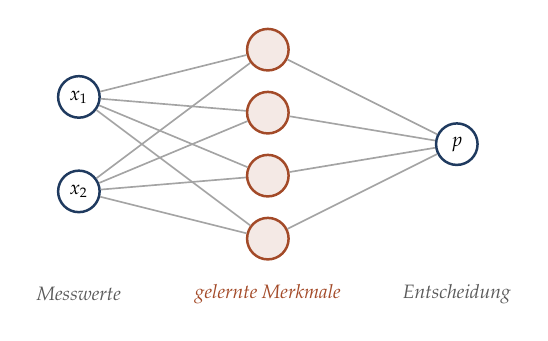
\begin{tikzpicture}[scale=1.0]
\foreach \i/\y in {1/1.8,2/0.6} \node[knotenb] (x\i) at (0,\y) {$x_\i$};
\foreach \j/\y in {1/2.4,2/1.6,3/0.8,4/0.0} \node[knotenr] (h\j) at (2.4,\y) {};
\node[knotenb] (p) at (4.8,1.2) {$p$};
\foreach \i in {1,2} \foreach \j in {1,2,3,4} \draw[grau!55, line width=0.6pt] (x\i)--(h\j);
\foreach \j in {1,2,3,4} \draw[grau!55, line width=0.6pt] (h\j)--(p);
\node[font=\scriptsize\itshape, color=grau] at (0,-0.7) {Messwerte};
\node[font=\scriptsize\itshape, color=akzent] at (2.4,-0.7) {gelernte Merkmale};
\node[font=\scriptsize\itshape, color=grau] at (4.8,-0.7) {Entscheidung};
\end{tikzpicture}
\end{center}

\begin{center}
{\small
\renewcommand{\arraystretch}{1.5}
\begin{tabular}{@{}P{2.6cm}P{6.0cm}@{}}
\toprule
\textbf{Die letzte Schicht} & ist eine logistische Regression --- auf den Merkmalen $\vek h$ statt auf $\vek x$.\\
\textbf{Die verdeckte Schicht} & erzeugt diese Merkmale, und zwar solche, mit denen die letzte Schicht gut arbeiten kann.\\
\textbf{Beide} & werden gemeinsam gelernt.\\
\bottomrule
\end{tabular}}
\end{center}

\begin{center}
\begin{minipage}{0.9\textwidth}
\textbf{Ein Netz ist eine logistische Regression, die ihre eigenen Merkmale erfindet.}
\end{minipage}
\end{center}
\end{merksatz}

\begin{merksatz}
\boxtitel{Wie zwei Gleichrichter eine Mulde bauen}
Mit $u = T - 37$:
\[ \max\{0,\ u - 1\} + \max\{0,\ -u - 1\} \]

\begin{center}
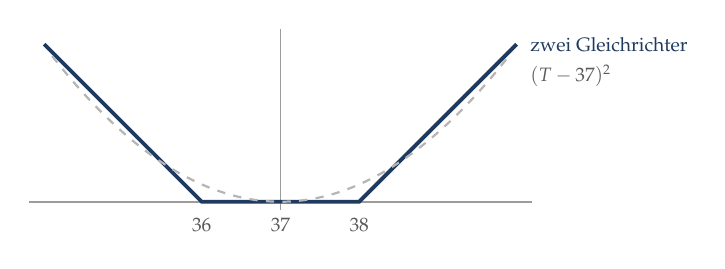
\begin{tikzpicture}[scale=1.0]
\draw[grau!60, line width=0.6pt] (-3.2,0) -- (3.2,0);
\draw[grau!60, line width=0.6pt] (0,-0.1) -- (0,2.2);
\draw[tief, line width=1.4pt] (-3,2) -- (-1,0) -- (1,0) -- (3,2);
\draw[grau!45, line width=0.8pt, dashed, smooth, samples=40, domain=-2.9:2.9] plot ({\x}, {0.22*\x*\x});
\node[font=\scriptsize, color=grau, anchor=north] at (-1,-0.08) {$36$};
\node[font=\scriptsize, color=grau, anchor=north] at (1,-0.08) {$38$};
\node[font=\scriptsize, color=grau, anchor=north] at (0,-0.08) {$37$};
\node[font=\scriptsize, color=tief, anchor=west] at (3.05,2) {zwei Gleichrichter};
\node[font=\scriptsize, color=grau, anchor=west] at (3.05,1.6) {$(T-37)^{2}$};
\end{tikzpicture}
\end{center}

\begin{center}
\begin{minipage}{0.88\textwidth}
\kursiv{\textbf{Das ist das klinische Kriterium \enquote{über $38$ oder unter $36$} als Funktion}, gebaut aus zwei Gleichrichtern --- einer für das Fieber, einer für die Untertemperatur. Ein Netz mit zwei verdeckten Einheiten kann dieses Merkmal lernen. Ob es das tut, ist eine andere Frage, und der Leitfall beantwortet sie.}
\end{minipage}
\end{center}
\end{merksatz}

\begin{merksatz}
\boxtitel{Satz 11.2 --- universelle Näherung}
Jede stetige Funktion auf einem beschränkten Bereich lässt sich durch ein Netz mit einer verdeckten Schicht beliebig genau nähern --- sofern man genug verdeckte Einheiten zulässt.

\begin{center}
\begin{minipage}{0.88\textwidth}
\kursiv{Der Beweis für die logistische Funktion stammt von \Person{George Cybenko} (1989) und benutzt den Satz von Hahn-Banach aus Band 13. Wir verzichten auf ihn --- die siebte Auslassung. \textbf{Für Gleichrichter ist der Gedanke anschaulich}: Aus zwei Gleichrichtern baut man eine Mulde, aus vier einen Buckel, aus vielen Buckeln jede Kurve --- wie ein Histogramm aus Säulen.}
\end{minipage}
\end{center}

\schritt{Was der Satz nicht sagt}
\begin{center}
{\small
\renewcommand{\arraystretch}{1.5}
\begin{tabular}{@{}P{2.4cm}P{6.2cm}@{}}
\toprule
\textbf{Wie viele} & Es können astronomisch viele Einheiten nötig sein.\\
\textbf{Wie finden} & Er sagt nicht, wie man die Gewichte findet.\\
\textbf{Wie verallgemeinern} & Er sagt nichts über ungesehene Daten.\\
\bottomrule
\end{tabular}}
\end{center}

\begin{center}
\begin{minipage}{0.88\textwidth}
\kursiv{\textbf{Der Satz ist eine Aussage über Darstellbarkeit, nicht über Lernbarkeit.} Auch Polynome können jede stetige Funktion nähern (Weierstraß, Band 3), und Kapitel~2 zeigte, wie das beim Lernen ausgeht. Die Bedeutung des Satzes wird oft überschätzt.}
\end{minipage}
\end{center}
\end{merksatz}

\section{Rückpropagation}

\begin{merksatz}
\boxtitel{Wie man die Gewichte findet}
Man minimiert die Kreuzentropie aus Kapitel~5 über alle Gewichte durch Gradientenabstieg. Gebraucht wird die Ableitung nach jedem Gewicht.

\schritt{Die Kettenregel, rückwärts angewandt}
Für das Netz aus Definition 11.1 mit einem Patienten:

\begin{center}
{\small
\renewcommand{\arraystretch}{1.6}
\begin{tabular}{@{}P{2.8cm}P{5.8cm}@{}}
\toprule
\textbf{Ausgang} & $\delta_2 = \dfrac{\partial\ell}{\partial z_2} = p - y$ \quad (Satz 5.2)\\
\textbf{letzte Gewichte} & $\dfrac{\partial\ell}{\partial\vek w_2} = \delta_2\,\vek h$\\
\textbf{zurück in die Schicht} & $\dfrac{\partial\ell}{\partial\vek h} = \delta_2\,\vek w_2$\\
\textbf{durch die Aktivierung} & $\vek\delta_1 = \dfrac{\partial\ell}{\partial\vek h}\odot g'(\vek z_1)$\\
\textbf{erste Gewichte} & $\dfrac{\partial\ell}{\partial W_1} = \vek\delta_1\,\vek x^{\!\top}$\\
\bottomrule
\end{tabular}}
\end{center}
\kursiv{$\odot$ bedeutet Multiplikation Eintrag für Eintrag.}

\begin{center}
\begin{minipage}{0.9\textwidth}
\textbf{Der Fehler am Ausgang wird Schicht für Schicht zurückgereicht --- gewichtet mit den Verbindungen, gedämpft durch die Ableitungen.}
\end{minipage}
\end{center}

\begin{center}
\begin{minipage}{0.88\textwidth}
\kursiv{Der Rechenaufwand ist bemerkenswert: \textbf{Alle Ableitungen zusammen kosten nur etwa doppelt so viel wie eine Vorhersage} --- unabhängig von der Zahl der Gewichte. Würde man jede Ableitung einzeln durch eine kleine Änderung annähern, bräuchte man eine Vorhersage je Gewicht, bei Millionen von Gewichten also Millionen. Ohne diese Einsparung gäbe es keine großen Netze.}
\end{minipage}
\end{center}
\end{merksatz}

\section{Kein Tal, sondern ein Gebirge}

\begin{warnung}
\boxtitelr{Die Konvexität ist verloren}
Die Kreuzentropie war in Kapitel~5 konvex --- ein einziges Tal. Im Netz ist sie es nicht mehr.

\schritt{Erster Grund: Vertauschungen}
Vertauscht man zwei verdeckte Einheiten samt ihren Gewichten, so rechnet das Netz dasselbe. Bei $m$ Einheiten gibt es $m!$ gleichwertige Lösungen.

\begin{center}
{\small
\renewcommand{\arraystretch}{1.46}
\begin{tabular}{@{}P{2.4cm}P{4.0cm}@{}}
\toprule
$m$ & \textbf{gleichwertige Minima}\\
\midrule
$4$ & $24$\\
$16$ & $2{,}1\cdot10^{13}$\\
\bottomrule
\end{tabular}}
\end{center}

\begin{center}
\begin{minipage}{0.88\textwidth}
\kursiv{Eine konvexe Funktion hat höchstens ein Tal. \textbf{Eine Funktion mit $10^{13}$ getrennten Tälern ist nicht konvex}, und zwischen ihnen liegen Pässe und Grate. Ob man in einem guten Tal landet, hängt vom Ausgangspunkt ab.}
\end{minipage}
\end{center}

\schritt{Zweiter Grund: schlechte Täler}
Neben den gleichwertigen gibt es auch schlechtere Minima. Im Leitfall mit zwei verdeckten Einheiten:

\begin{center}
{\small
\renewcommand{\arraystretch}{1.46}
\begin{tabular}{@{}P{2.8cm}P{3.0cm}@{}}
\toprule
\textbf{Zufallsstart} & \textbf{Testfehler}\\
\midrule
bester von fünf & $4{,}2\,\%$\\
schlechtester & $20{,}2\,\%$\\
\bottomrule
\end{tabular}}
\end{center}

\begin{center}
\begin{minipage}{0.88\textwidth}
\kursiv{Der schlechteste Start endet bei \enquote{nie warnen}. \textbf{Das Netz könnte die Mulde bauen, findet sie aber nicht}, weil der Gradientenabstieg in einem Tal stecken bleibt, in dem beide Einheiten dasselbe tun oder gar nichts. Die Darstellbarkeit aus Satz 11.2 hilft nicht, wenn der Weg dorthin versperrt ist.}
\end{minipage}
\end{center}
\end{warnung}

\section{Der Leitfall gerechnet}

\begin{merksatz}
\boxtitel{Netze verschiedener Breite}
$300$ Patienten, Gleichrichter, leichte Strafe auf die Gewichte, je fünf Zufallsstarts:

\begin{center}
{\small
\renewcommand{\arraystretch}{1.46}
\begin{tabular}{@{}P{1.6cm}P{1.8cm}P{2.8cm}P{1.8cm}@{}}
\toprule
\textbf{Einh.} & \textbf{Training} & \textbf{Test (Spannweite)} & \textbf{Trennsch.}\\
\midrule
$1$ & $12{,}1\,\%$ & $13{,}0$ ($8$--$20$) & $0{,}743$\\
$2$ & $13{,}0\,\%$ & $13{,}9$ ($4$--$20$) & $0{,}825$\\
$4$ & $3{,}6\,\%$ & $4{,}3$ ($3$--$8$) & $0{,}993$\\
$16$ & $2{,}4\,\%$ & $2{,}7$ ($2{,}6$--$2{,}9$) & $\mathbf{0{,}994}$\\
$64$ & $2{,}3\,\%$ & $2{,}6$ ($2{,}5$--$2{,}6$) & $\mathbf{0{,}994}$\\
\bottomrule
\end{tabular}}
\end{center}

\begin{center}
\begin{minipage}{0.9\textwidth}
\textbf{Ab sechzehn Einheiten erreicht das Netz die Trennschärfe des von Hand erfundenen Merkmals --- $0{,}994$.}
\end{minipage}
\end{center}

\schritt{Zwei Beobachtungen}
\begin{center}
{\small
\renewcommand{\arraystretch}{1.5}
\begin{tabular}{@{}P{2.6cm}P{6.0cm}@{}}
\toprule
\textbf{Mehr ist stabiler} & Bei zwei Einheiten streut das Ergebnis zwischen $4$ und $20$ Prozent, bei sechzehn kaum noch.\\
\textbf{Mehr schadet nicht} & Selbst ein Netz mit zwei Schichten zu je $256$ Einheiten --- $66\,817$ Gewichte für $300$ Patienten, ohne jede Strafe --- erreicht $2{,}7$ Prozent.\\
\bottomrule
\end{tabular}}
\end{center}

\begin{center}
\begin{minipage}{0.88\textwidth}
\kursiv{\textbf{Die zweite Zeile widerspricht allem, was Teil~I und III lehren.} Zweihundertmal mehr Gewichte als Patienten, und keine Überanpassung. Nach Satz 2.2 wäre der Optimismus riesig, nach Satz 7.6 die Schranke nichtssagend --- und doch verallgemeinert das Netz. Die erste Zeile gibt einen Hinweis: Breite Netze haben so viele gute Täler, dass der Gradientenabstieg fast immer eines findet. Kapitel~14 nimmt die Frage wieder auf.}
\end{minipage}
\end{center}
\end{merksatz}

\section{Der Bruchfall}

\begin{warnung}
\boxtitelr{Der verschwindende Gradient}
Bei der Rückpropagation wird der Fehler in jeder Schicht mit $g'(z)$ multipliziert. Für die logistische Funktion ist $g' \le \tfrac14$.

\begin{center}
{\small
\renewcommand{\arraystretch}{1.46}
\begin{tabular}{@{}P{2.0cm}P{3.0cm}@{}}
\toprule
\textbf{Schichten} & \textbf{höchstens $(\tfrac14)^{L}$}\\
\midrule
$2$ & $0{,}0625$\\
$5$ & $9{,}8\cdot10^{-4}$\\
$10$ & $9{,}5\cdot10^{-7}$\\
\bottomrule
\end{tabular}}
\end{center}

\begin{center}
\begin{minipage}{0.9\textwidth}
\textbf{In einem Netz mit zehn logistischen Schichten erreicht die erste Schicht höchstens ein Millionstel des Fehlersignals.}
\end{minipage}
\end{center}

\begin{center}
\begin{minipage}{0.88\textwidth}
\kursiv{Die vorderen Schichten lernen dann praktisch nichts. \textbf{Das war der Hauptgrund, warum tiefe Netze bis etwa 2010 nicht funktionierten.} Der Gleichrichter hat die Ableitung $1$ auf seiner aktiven Seite und reicht das Signal ungedämpft weiter; zusammen mit sorgfältiger Wahl der Anfangsgewichte machte er tiefe Netze erst trainierbar.}
\end{minipage}
\end{center}
\end{warnung}

\begin{warnung}
\boxtitelr{Was sonst noch schiefgeht}
\begin{center}
{\small
\renewcommand{\arraystretch}{1.52}
\begin{tabular}{@{}P{2.6cm}P{6.0cm}@{}}
\toprule
\textbf{Stellgrößen} & Zahl der Schichten und Einheiten, Schrittweite, Strafe, Abbruchzeit, Anfangswerte --- jede beeinflusst das Ergebnis.\\
\textbf{Zu sicher} & Große Netze geben oft Wahrscheinlichkeiten nahe null oder eins aus, die zu extrem sind.\\
\textbf{Außerhalb} & Gleichrichternetze setzen außerhalb der Daten linear fort --- ohne Grenze und ohne Warnung.\\
\bottomrule
\end{tabular}}
\end{center}

\begin{center}
\begin{minipage}{0.88\textwidth}
\kursiv{Die zweite Zeile ist für die Medizin die ernsteste. \textbf{Ein Netz, das \enquote{Sepsis mit $99$ Prozent} ausgibt, ist womöglich nur zu $80$ Prozent sicher} --- und nach Kapitel~1 hängt die richtige Entscheidung von der Wahrscheinlichkeit ab, nicht nur vom Urteil. Man muss die Kalibrierung nachträglich prüfen und korrigieren, was bei der logistischen Regression kaum nötig ist.}
\end{minipage}
\end{center}
\end{warnung}

\section{Übungsaufgaben}

\begin{aufgabe}
\boxtitel{Aufgabe 11.1 --- XOR mit zwei Gleichrichtern}
Zeigen Sie, dass das Netz
\[ h_1 = \max\{0,\ x_1+x_2\}, \qquad h_2 = \max\{0,\ x_1+x_2-1\}, \qquad f = h_1 - 2\,h_2 \]
das XOR-Problem auf $\{0,1\}^{2}$ löst.

\loesung
\schritt{Schritt 1 --- Alle vier Eingaben}
\begin{center}
{\small
\renewcommand{\arraystretch}{1.5}
\begin{tabular}{@{}P{1.4cm}P{1.6cm}P{1.2cm}P{1.2cm}P{2.0cm}P{1.2cm}@{}}
\toprule
$(x_1,x_2)$ & $x_1+x_2$ & $h_1$ & $h_2$ & $h_1-2h_2$ & \textbf{XOR}\\
\midrule
$(0,0)$ & $0$ & $0$ & $0$ & $0$ & $0$\\
$(1,0)$ & $1$ & $1$ & $0$ & $1$ & $1$\\
$(0,1)$ & $1$ & $1$ & $0$ & $1$ & $1$\\
$(1,1)$ & $2$ & $2$ & $1$ & $0$ & $0$\\
\bottomrule
\end{tabular}}
\end{center}

Alle vier stimmen. \checkmark

\schritt{Schritt 2 --- Was die Einheiten tun}
\begin{center}
{\small
\renewcommand{\arraystretch}{1.5}
\begin{tabular}{@{}P{1.6cm}P{6.8cm}@{}}
\toprule
$h_1$ & zählt, wie viele Merkmale zutreffen.\\
$h_2$ & meldet sich erst, wenn beide zutreffen.\\
$f$ & zieht den doppelten Beitrag von $h_2$ ab --- \enquote{eines, aber nicht beide}.\\
\bottomrule
\end{tabular}}
\end{center}

\schritt{Schritt 3 --- Die Einordnung}
\begin{center}
\begin{minipage}{0.88\textwidth}
\kursiv{Kapitel~6 löste XOR mit dem Merkmal $x_1x_2$, das ein Mensch wählte. \textbf{Hier entsteht dasselbe aus zwei Einheiten}, deren Gewichte man lernen kann: $h_2$ ist im Wesentlichen das Produkt $x_1x_2$ auf $\{0,1\}^{2}$. Minsky und Papert wussten 1969, dass eine verdeckte Schicht XOR löst; es fehlte ein Verfahren, die Gewichte zu finden --- die Rückpropagation.}
\end{minipage}
\end{center}
\end{aufgabe}

\begin{aufgabe}
\boxtitel{Aufgabe 11.2 --- Rückpropagation von Hand}
Ein Netz mit einem Eingang, einer logistischen verdeckten Einheit und logistischem Ausgang. Gewichte $w_1 = 0{,}5$, $b_1 = 0$, $w_2 = 1$, $b_2 = 0$. Ein Patient: $x = 1$, $y = 1$. Berechnen Sie alle Ableitungen und einen Schritt mit $\eta = 1$.

\loesung
\schritt{Schritt 1 --- Vorwärts}
\begin{align*}
z_1 &= 0{,}5\cdot1 + 0 = 0{,}5, & h &= \sigma(0{,}5) = 0{,}6225\\
z_2 &= 1\cdot0{,}6225 + 0 = 0{,}6225, & p &= \sigma(0{,}6225) = 0{,}6508\\
\ell &= -\ln0{,}6508 = 0{,}4296
\end{align*}

\schritt{Schritt 2 --- Rückwärts: Ausgang}
\[ \delta_2 = p - y = 0{,}6508 - 1 = -0{,}3492 \]
\[ \frac{\partial\ell}{\partial w_2} = \delta_2\,h = -0{,}3492\cdot0{,}6225 = -0{,}2174, \qquad \frac{\partial\ell}{\partial b_2} = -0{,}3492 \]

\schritt{Schritt 3 --- Rückwärts: verdeckte Einheit}
\[ \frac{\partial\ell}{\partial h} = \delta_2\,w_2 = -0{,}3492 \]
\[ \sigma'(z_1) = h\,(1-h) = 0{,}6225\cdot0{,}3775 = 0{,}2350 \]
\[ \delta_1 = -0{,}3492\cdot0{,}2350 = -0{,}0821 \]
\[ \frac{\partial\ell}{\partial w_1} = \delta_1\,x = -0{,}0821, \qquad \frac{\partial\ell}{\partial b_1} = -0{,}0821 \]

\schritt{Schritt 4 --- Die Probe durch Nachrechnen}
Man ändere $w_1$ um $\pm10^{-6}$ und bilde den Differenzenquotienten des Verlusts:
\[ \frac{\ell(0{,}500001) - \ell(0{,}499999)}{0{,}000002} = -0{,}0821 \quad \checkmark \]
Ebenso für $w_2$: $-0{,}2174$. \checkmark

\schritt{Schritt 5 --- Ein Schritt}
\begin{center}
{\small
\renewcommand{\arraystretch}{1.48}
\begin{tabular}{@{}P{1.6cm}P{1.6cm}P{2.2cm}P{1.8cm}@{}}
\toprule
\textbf{Gewicht} & \textbf{alt} & \textbf{Ableitung} & \textbf{neu}\\
\midrule
$w_1$ & $0{,}500$ & $-0{,}0821$ & $0{,}582$\\
$b_1$ & $0{,}000$ & $-0{,}0821$ & $0{,}082$\\
$w_2$ & $1{,}000$ & $-0{,}2174$ & $1{,}217$\\
$b_2$ & $0{,}000$ & $-0{,}3492$ & $0{,}349$\\
\bottomrule
\end{tabular}}
\end{center}

\[ \ell_{\text{neu}} = 0{,}2744 \quad\text{statt}\quad 0{,}4296 \]

\begin{center}
\begin{minipage}{0.88\textwidth}
\kursiv{\textbf{Die vordere Schicht bekommt ein Viertel des Signals der hinteren} --- $0{,}082$ gegen $0{,}349$ ---, und der Faktor ist genau $\sigma'(z_1)\cdot w_2 = 0{,}235$. Das ist der verschwindende Gradient aus dem Bruchfall, schon bei einer einzigen Schicht sichtbar.}
\end{minipage}
\end{center}
\end{aufgabe}

\begin{aufgabe}
\boxtitel{Aufgabe 11.3 --- Wie viele Gewichte?}
Zählen Sie die Gewichte eines Netzes mit zwei Eingängen, zwei verdeckten Schichten zu je $h$ Einheiten und einem Ausgang, und vergleichen Sie mit der Zahl der Patienten.

\loesung
\schritt{Schritt 1 --- Schicht für Schicht}
\begin{center}
{\small
\renewcommand{\arraystretch}{1.5}
\begin{tabular}{@{}P{3.0cm}P{2.4cm}P{2.4cm}@{}}
\toprule
\textbf{Verbindung} & \textbf{Gewichte} & \textbf{Achsenabschn.}\\
\midrule
Eingang $\to$ Schicht 1 & $2h$ & $h$\\
Schicht 1 $\to$ Schicht 2 & $h^{2}$ & $h$\\
Schicht 2 $\to$ Ausgang & $h$ & $1$\\
\bottomrule
\end{tabular}}
\end{center}

\[ \text{zusammen: } h^{2} + 5h + 1 \]

\schritt{Schritt 2 --- Die Zahlen}
\begin{center}
{\small
\renewcommand{\arraystretch}{1.48}
\begin{tabular}{@{}P{1.6cm}P{2.4cm}P{3.4cm}@{}}
\toprule
$h$ & \textbf{Gewichte} & \textbf{je Patient ($n = 300$)}\\
\midrule
$4$ & $37$ & $0{,}12$\\
$16$ & $337$ & $1{,}1$\\
$64$ & $4417$ & $15$\\
$256$ & $66\,817$ & $223$\\
\bottomrule
\end{tabular}}
\end{center}

\kursiv{Probe für $h = 64$:} $4096 + 320 + 1 = 4417$. \checkmark

\schritt{Schritt 3 --- Was die Faustregel sagt}
\begin{center}
\begin{minipage}{0.88\textwidth}
\kursiv{Nach Aufgabe 2.3 bräuchte man zehn Ereignisse je Parameter. Mit $60$ Sepsisfällen erlaubt das sechs Parameter --- \textbf{das kleinste Netz der Tabelle hat bereits sechsmal so viele}, das größte zehntausendmal. Und doch verallgemeinert das größte so gut wie das Netz mit sechzehn Einheiten.}
\end{minipage}
\end{center}

\begin{center}
\begin{minipage}{0.88\textwidth}
\kursiv{\textbf{Die Faustregel gilt für die logistische Regression, und dort gilt sie gut.} Für Netze gilt sie nicht, und zwar nicht, weil Netze besser wären, sondern weil ihre Parameter nicht unabhängig voneinander wirken und der Gradientenabstieg nicht jede Lösung gleich wahrscheinlich findet. Die Zahl der Gewichte ist bei Netzen kein brauchbares Maß der Komplexität --- und ein besseres gibt es noch nicht.}
\end{minipage}
\end{center}
\end{aufgabe}

\begin{geschichte}
\boxtitelg{Die Rückpropagation, mehrmals erfunden}
\begin{center}
{\small
\renewcommand{\arraystretch}{1.5}
\begin{tabular}{@{}P{1.4cm}P{2.8cm}P{4.2cm}@{}}
\toprule
\textbf{Jahr} & \textbf{Wer} & \textbf{Wo}\\
\midrule
$1970$ & \Person{Seppo Linnainmaa} & Rundungsfehler, finnische Magisterarbeit\\
$1974$ & \Person{Paul Werbos} & Dissertation, Harvard\\
$1986$ & \Person{Rumelhart}, \Person{Hinton}, \Person{Williams} & \kursiv{Nature}, drei Seiten\\
\bottomrule
\end{tabular}}
\end{center}

\begin{center}
\begin{minipage}{0.9\textwidth}
\kursiv{Linnainmaa entwickelte das rückwärts angewandte automatische Differenzieren für ganz andere Zwecke. Werbos wandte es 1974 auf Netze an; seine Arbeit fand kaum Beachtung. \textbf{Erst der Aufsatz von 1986 machte das Verfahren bekannt} --- nicht weil er neu war, sondern weil er zeigte, dass die verdeckten Einheiten sinnvolle Merkmale lernten.}
\end{minipage}
\end{center}

\schritt{Die zweite Rückkehr}
\begin{center}
\begin{minipage}{0.9\textwidth}
\kursiv{In den 1990er Jahren verloren die Netze wieder an Boden --- gegen Stützvektormaschinen, deren Theorie sauberer war. \Person{Geoffrey Hinton}, \Person{Yoshua Bengio} und \Person{Yann LeCun} arbeiteten weiter, oft gegen den Widerstand der Gutachter. \textbf{2012 gewann ein tiefes Netz aus Hintons Gruppe einen Bilderkennungswettbewerb mit großem Abstand} --- und innerhalb von zwei Jahren wechselte fast das ganze Fach. Die drei erhielten 2018 den Turing-Preis.}
\end{minipage}
\end{center}

\schritt{Und ein Nobelpreis}
\begin{center}
\begin{minipage}{0.9\textwidth}
\kursiv{2024 erhielten \Person{John Hopfield} und Hinton den Nobelpreis für Physik --- für Beiträge zu Netzen, die aus der statistischen Physik stammen. \textbf{Es war das erste Mal, dass der Physikpreis für eine Arbeit vergeben wurde, deren Hauptanwendung im maschinellen Lernen liegt}, und die Entscheidung wurde im Fach kontrovers aufgenommen.}
\end{minipage}
\end{center}
\end{geschichte}

\begin{forschung}
\boxtitelp{Netze heute}
\begin{center}
{\small
\renewcommand{\arraystretch}{1.45}
\begin{tabular}{@{}P{2.8cm}P{5.4cm}@{}}
\toprule
\textbf{Automatisches Differenzieren} & Rückpropagation für beliebige Programme --- die Grundlage aller heutigen Werkzeuge.\\
\textbf{Tabellen} & Bei tabellarischen klinischen Daten sind Netze den Wäldern meist unterlegen.\\
\textbf{Kalibrierung} & Verfahren, zu sichere Netze nachträglich abzuschwächen.\\
\bottomrule
\end{tabular}}
\end{center}

\schritt{Zur zweiten Zeile}
\begin{center}
\begin{minipage}{0.88\textwidth}
\kursiv{Mehrere große Vergleichsstudien seit 2021 fanden, dass Gradient-Boosting aus Kapitel~9 auf Tabellendaten mittlerer Größe tiefe Netze meist schlägt. \textbf{Netze glänzen bei Bildern, Tönen und Texten}, wo die Merkmale aus Rohdaten erst gebildet werden müssen. Bei Laborwerten, die schon sinnvolle Merkmale sind, bringt diese Fähigkeit wenig --- und Netze zahlen den Preis der Nichtkonvexität umsonst.}
\end{minipage}
\end{center}
\end{forschung}

\begin{merksatz}
\boxtitel{Was Sie jetzt können}
\begin{center}
\renewcommand{\arraystretch}{1.5}
\begin{tabular}{@{}P{3.0cm}P{5.6cm}@{}}
\toprule
\textbf{Definition 11.1} & logistische Regression, die Merkmale erfindet\\
\textbf{Satz 11.2} & alles darstellbar --- aber nicht alles findbar\\
\textbf{Rückpropagation} & Kettenregel rückwärts, doppelte Vorhersagekosten\\
\textbf{Nichtkonvexität} & $m!$ Täler, manche schlecht\\
\textbf{Der Bruchfall} & $(\tfrac14)^{L}$ --- darum Gleichrichter\\
\bottomrule
\end{tabular}
\end{center}

\begin{center}
\begin{minipage}{0.88\textwidth}
\kursiv{Damit endet Teil~IV. Alle bisherigen Verfahren brauchten Etiketten --- Sepsis ja oder nein. Teil~V fragt, was man lernen kann, wenn niemand sagt, was richtig ist.}
\end{minipage}
\end{center}
\end{merksatz}

\part{Ohne Etiketten, in der Tiefe}

\chapter{Gruppen finden}

\section{Der Leitfall}

\begin{merksatz}
\boxtitel{Gibt es verschiedene Arten von Sepsis?}
Alle bisherigen Kapitel hatten ein Etikett: Sepsis ja oder nein. Nun stellt das Klinikum eine andere Frage: \kursiv{Unter} den Sepsispatienten --- gibt es Untergruppen, die sich verschieden verhalten und vielleicht verschieden behandelt werden sollten?

\begin{center}
\begin{minipage}{0.9\textwidth}
\textbf{Niemand kennt die Antwort. Es gibt keine Etiketten, aus denen man lernen könnte.}
\end{minipage}
\end{center}

\begin{center}
\begin{minipage}{0.88\textwidth}
\kursiv{Die Frage ist nicht erfunden. \textbf{Eine große Studie beschrieb 2019 vier Sepsis-Phänotypen}, gewonnen aus Routinedaten von über $20\,000$ Patienten --- ohne Vorgabe, wie viele Gruppen es geben sollte oder woran sie zu erkennen wären. Die Gruppen unterschieden sich deutlich in der Sterblichkeit. Dieses Kapitel zeigt, wie solche Gruppen gefunden werden, und warum man ihnen mit Vorsicht begegnen sollte.}
\end{minipage}
\end{center}
\end{merksatz}

\begin{merksatz}
\boxtitel{Überwacht und unüberwacht}
\begin{center}
{\small
\renewcommand{\arraystretch}{1.55}
\begin{tabular}{@{}P{2.6cm}P{3.0cm}P{3.0cm}@{}}
\toprule
& \textbf{überwacht} & \textbf{unüberwacht}\\
\midrule
Daten & $(\vek x_i, y_i)$ & nur $\vek x_i$\\
Ziel & $y$ vorhersagen & Struktur finden\\
Prüfung & Testfehler & \textcolor{akzent}{?}\\
\bottomrule
\end{tabular}}
\end{center}

\begin{center}
\begin{minipage}{0.88\textwidth}
\kursiv{Das Fragezeichen ist der Kern der Schwierigkeit. \textbf{Beim überwachten Lernen weiß man hinterher, ob man richtig lag} --- man vergleicht mit dem Etikett. Beim unüberwachten gibt es nichts zu vergleichen. Jedes Verfahren findet \kursiv{irgendwelche} Gruppen, und ob sie etwas bedeuten, lässt sich aus den Daten allein nicht entscheiden.}
\end{minipage}
\end{center}
\end{merksatz}

\section{Das Verfahren der $k$ Mittelpunkte}

\begin{definition}
\boxtitelm{Definition 12.1 --- die Zielgröße}
Teile $n$ Punkte in $k$ Gruppen $C_1,\ldots,C_k$ mit Mittelpunkten $\vek\mu_1,\ldots,\vek\mu_k$ so ein, dass die Summe der quadrierten Abstände zum eigenen Mittelpunkt
\[ W = \sum_{j=1}^{k}\ \sum_{\vek x_i\in C_j} \|\vek x_i - \vek\mu_j\|^{2} \]
möglichst klein wird.
\end{definition}

\begin{merksatz}
\boxtitel{Das Verfahren von Lloyd}
\begin{center}
{\small
\renewcommand{\arraystretch}{1.5}
\begin{tabular}{@{}P{1.0cm}P{7.4cm}@{}}
\toprule
$0$ & Wähle $k$ Anfangsmittelpunkte.\\
$1$ & \textbf{Zuordnen:} Jeder Punkt kommt zum nächsten Mittelpunkt.\\
$2$ & \textbf{Verschieben:} Jeder Mittelpunkt wird der Durchschnitt seiner Gruppe.\\
$3$ & Wiederhole $1$ und $2$, bis sich nichts mehr ändert.\\
\bottomrule
\end{tabular}}
\end{center}

\schritt{Satz 12.2 --- das Verfahren endet}
Keiner der beiden Schritte vergrößert $W$, und das Verfahren hält nach endlich vielen Schritten an.

\schritt{Beweis}
\kursiv{Zuordnen:} Jeder Punkt wechselt nur, wenn er dadurch einem Mittelpunkt näher kommt. Sein Beitrag zu $W$ sinkt oder bleibt gleich.

\kursiv{Verschieben:} Für eine feste Gruppe ist der Durchschnitt derjenige Punkt, der die Summe der quadrierten Abstände minimiert. Denn
\[ \sum_{i}\|\vek x_i - \vek c\|^{2} = \sum_i\|\vek x_i - \bar{\vek x}\|^{2} + n_j\,\|\bar{\vek x} - \vek c\|^{2} , \]
und der zweite Summand ist nur für $\vek c = \bar{\vek x}$ null. Das ist dieselbe Zerlegung wie in Aufgabe 2.1.

\kursiv{Endlichkeit:} Es gibt nur endlich viele Einteilungen von $n$ Punkten in $k$ Gruppen. Da $W$ nie steigt und bei jeder echten Änderung sinkt, kann keine Einteilung zweimal vorkommen. $\blacksquare$

\begin{center}
\begin{minipage}{0.9\textwidth}
\textbf{Das Verfahren endet stets --- aber nicht notwendig im besten Zustand.}
\end{minipage}
\end{center}

\begin{center}
\begin{minipage}{0.88\textwidth}
\kursiv{Es findet ein lokales Minimum, das von den Anfangsmittelpunkten abhängt. \textbf{Das globale Minimum zu finden, ist $\mathsf{NP}$-schwer} --- schon in der Ebene. Man startet deshalb viele Male mit verschiedenen Anfängen und behält das beste Ergebnis.}
\end{minipage}
\end{center}
\end{merksatz}

\section{Mischungen und das EM-Verfahren}

\begin{merksatz}
\boxtitel{Der Leitfall aus Kapitel 1 --- ohne Etiketten}
Man nehme $2000$ Laktatwerte aus der Verteilung von Kapitel~1, aber ohne die Angabe, wer eine Sepsis hatte.

\begin{center}
\begin{minipage}{0.9\textwidth}
\textbf{Kann man aus den Werten allein wiederfinden, dass es zwei Gruppen gibt, wie groß sie sind und wo sie liegen?}
\end{minipage}
\end{center}

\schritt{Das Modell}
Man nimmt an, die Werte stammten aus einer \Begriff{Mischung} zweier Normalverteilungen:
\[ f(x) = \pi\cdot\mathcal N(x;\mu_1,\sigma_1^{2}) + (1-\pi)\cdot\mathcal N(x;\mu_2,\sigma_2^{2}) \]
mit fünf unbekannten Größen.
\end{merksatz}

\begin{merksatz}
\boxtitel{Das Verfahren}
Man wiederholt zwei Schritte:

\begin{center}
{\small
\renewcommand{\arraystretch}{1.55}
\begin{tabular}{@{}P{2.4cm}P{6.2cm}@{}}
\toprule
\textbf{E-Schritt} & Berechne für jeden Punkt, mit welcher Wahrscheinlichkeit er zu Gruppe 2 gehört --- nach dem Satz von Bayes mit den jetzigen Schätzungen.\\
\textbf{M-Schritt} & Schätze die fünf Größen neu, wobei jeder Punkt mit dieser Wahrscheinlichkeit gewichtet wird.\\
\bottomrule
\end{tabular}}
\end{center}

\begin{center}
\begin{minipage}{0.88\textwidth}
\kursiv{\textbf{Der E-Schritt ist genau die Rechnung aus Kapitel~1}: die Wahrscheinlichkeit $\eta(x)$ einer Sepsis beim Laktatwert $x$. Nur kennt man die Verteilungen nicht, sondern benutzt die jeweils letzte Schätzung. Das Verfahren heißt nach den Anfangsbuchstaben von \enquote{Erwartung} und \enquote{Maximierung}.}
\end{minipage}
\end{center}

\schritt{Satz 12.3 --- Dempster, Laird und Rubin, 1977}
Kein Schritt verringert die Likelihood der Daten (Band 17, Kapitel~4).

\begin{center}
\begin{minipage}{0.88\textwidth}
\kursiv{Der Beweis benutzt die Jensensche Ungleichung aus Band 20 und zeigt, dass jeder Schritt eine untere Schranke der Log-Likelihood maximiert, die an der jetzigen Stelle anliegt; wir verzichten auf ihn --- die achte Auslassung. \textbf{Das Verfahren von Lloyd ist ein Grenzfall davon}: Setzt man alle Streuungen gleich und lässt sie gegen null gehen, so werden die Wahrscheinlichkeiten zu harten Zuordnungen.}
\end{minipage}
\end{center}
\end{merksatz}

\begin{merksatz}
\boxtitel{Das Ergebnis}
\begin{center}
{\small
\renewcommand{\arraystretch}{1.5}
\begin{tabular}{@{}P{2.6cm}P{1.8cm}P{1.8cm}P{2.0cm}@{}}
\toprule
& \textbf{wahr} & \textbf{EM} & \textbf{$k$-Mittel}\\
\midrule
Anteil Gruppe 2 & $0{,}100$ & $0{,}094$ & $0{,}093$\\
Mittel Gruppe 1 & $1{,}20$ & $1{,}22$ & $1{,}21$\\
Mittel Gruppe 2 & $3{,}00$ & $3{,}23$ & $3{,}34$\\
Streuung Gruppe 1 & $0{,}50$ & $0{,}48$ & ---\\
Streuung Gruppe 2 & $1{,}00$ & $0{,}91$ & ---\\
\bottomrule
\end{tabular}}
\end{center}

\begin{center}
\begin{minipage}{0.9\textwidth}
\textbf{Ohne ein einziges Etikett findet das Verfahren beide Gruppen, ihre Größe und ihre Lage --- und ordnet $97$ Prozent der Patienten richtig zu.}
\end{minipage}
\end{center}

\begin{center}
\begin{minipage}{0.88\textwidth}
\kursiv{Die Bayes-Regel aus Kapitel~1 --- mit Kenntnis der wahren Verteilungen --- ordnete $96{,}5$ Prozent richtig zu. \textbf{Das unüberwachte Verfahren ist also fast so gut wie das bestmögliche überwachte.} Der Grund: Die Gruppen sind hier tatsächlich verschieden verteilt, und das Modell der Mischung trifft genau zu. Beides ist in der Wirklichkeit selten so klar.}
\end{minipage}
\end{center}
\end{merksatz}

\section{Wie viele Gruppen?}

\begin{warnung}
\boxtitelr{Das Verfahren findet immer Gruppen}
Zwei Datensätze mit je $500$ Punkten in der Ebene:

\begin{center}
{\small
\renewcommand{\arraystretch}{1.5}
\begin{tabular}{@{}P{2.8cm}P{5.8cm}@{}}
\toprule
\textbf{strukturiert} & drei deutlich getrennte Haufen\\
\textbf{gleichverteilt} & keinerlei Struktur, gleichmäßig über ein Quadrat gestreut\\
\bottomrule
\end{tabular}}
\end{center}

\begin{center}
{\small
\renewcommand{\arraystretch}{1.46}
\begin{tabular}{@{}P{1.2cm}P{2.2cm}P{2.2cm}P{1.4cm}P{1.4cm}@{}}
\toprule
& \multicolumn{2}{c}{\textbf{$W$}} & \multicolumn{2}{c}{\textbf{Stabilität}}\\
$k$ & strukturiert & gleichv. & str. & gl.\\
\midrule
$1$ & $218{,}9$ & $81{,}8$ & --- & ---\\
$2$ & $109{,}3$ & $49{,}2$ & $1{,}00$ & $0{,}68$\\
$3$ & $\mathbf{24{,}5}$ & $30{,}1$ & $\mathbf{1{,}00}$ & $0{,}71$\\
$4$ & $21{,}5$ & $20{,}0$ & $0{,}80$ & $\mathbf{0{,}85}$\\
$5$ & $18{,}7$ & $16{,}6$ & $0{,}66$ & $0{,}71$\\
\bottomrule
\end{tabular}}
\end{center}
\kursiv{Stabilität: Übereinstimmung der Gruppen über $20$ Neuziehungen, gemessen mit dem bereinigten Rand-Index --- $1$ heißt immer gleich.}

\begin{center}
\begin{minipage}{0.9\textwidth}
\textbf{Bei den strukturierten Daten knickt $W$ bei $k = 3$ deutlich ein. Bei den gleichverteilten fällt es gleichmäßig --- aber das Verfahren liefert trotzdem bei jedem $k$ genau $k$ Gruppen.}
\end{minipage}
\end{center}

\schritt{Und die Stabilität}
\begin{center}
\begin{minipage}{0.88\textwidth}
\kursiv{Man erwartet, dass echte Gruppen stabil sind und erfundene nicht. Bei den strukturierten Daten stimmt das: $1{,}00$ bei $k = 3$. \textbf{Bei den gleichverteilten Daten ist $k = 4$ mit $0{,}85$ am stabilsten} --- weil ein Quadrat vier Ecken hat und das Verfahren es zuverlässig in vier Viertel teilt. Die Stabilität misst, ob die Einteilung von der Stichprobe abhängt, nicht, ob es die Gruppen gibt.}
\end{minipage}
\end{center}
\end{warnung}

\section{Der Bruchfall}

\begin{warnung}
\boxtitelr{Was eine Gruppe ist}
\begin{center}
{\small
\renewcommand{\arraystretch}{1.52}
\begin{tabular}{@{}P{2.4cm}P{6.2cm}@{}}
\toprule
\textbf{Form} & $k$-Mittel findet runde Gruppen gleicher Größe. Langgestreckte oder verschachtelte übersieht es.\\
\textbf{Einheiten} & Wie in Kapitel~10: Die Wahl des Abstands entscheidet alles.\\
\textbf{Übergänge} & Ein Kontinuum wird in Stücke geschnitten, die es nicht gibt.\\
\bottomrule
\end{tabular}}
\end{center}

\schritt{Zur dritten Zeile}
\begin{center}
\begin{minipage}{0.88\textwidth}
\kursiv{Verläuft eine Erkrankung auf einem Kontinuum von leicht bis schwer, so findet ein Gruppierungsverfahren trotzdem \enquote{leichte}, \enquote{mittlere} und \enquote{schwere} Fälle --- als wären es verschiedene Arten. \textbf{Die Gruppen sind dann Schnitte durch eine Linie, keine Naturgegebenheiten.} In der Psychiatrie ist diese Frage seit Jahrzehnten umstritten: Sind Störungsbilder Kategorien oder Enden von Dimensionen? Gruppierungsverfahren beantworten sie nicht, sie setzen die Antwort voraus.}
\end{minipage}
\end{center}

\schritt{Was die Sepsis-Phänotypen zeigen}
\begin{center}
\begin{minipage}{0.88\textwidth}
\kursiv{Die vier Gruppen von 2019 unterschieden sich in der Sterblichkeit, und in Nachauswertungen früherer Studien schienen sie verschieden auf Behandlungen anzusprechen. \textbf{Das ist ein starkes Argument, dass sie etwas bedeuten} --- denn es ist eine Prüfung an einer Größe, die in die Gruppierung nicht einging. Ob es sich um verschiedene Krankheiten handelt oder um verschiedene Stadien, ist damit nicht entschieden. Und ob eine prospektive Behandlung nach Phänotyp besser wäre, müsste eigens geprüft werden.}
\end{minipage}
\end{center}
\end{warnung}

\section{Übungsaufgaben}

\begin{aufgabe}
\boxtitel{Aufgabe 12.1 --- Das Verfahren von Hand}
Sechs Laktatwerte: $1{,}0$; $1{,}2$; $1{,}5$; $2{,}8$; $3{,}1$; $3{,}6$. Zwei Gruppen, Anfangsmittelpunkte $1{,}0$ und $1{,}5$.

\loesung
\schritt{Runde 1 --- Zuordnen}
\begin{center}
{\small
\renewcommand{\arraystretch}{1.46}
\begin{tabular}{@{}P{1.4cm}P{2.2cm}P{2.2cm}P{1.4cm}@{}}
\toprule
$x$ & \textbf{Abstand zu $1{,}0$} & \textbf{Abstand zu $1{,}5$} & \textbf{Gruppe}\\
\midrule
$1{,}0$ & $0$ & $0{,}5$ & $1$\\
$1{,}2$ & $0{,}2$ & $0{,}3$ & $1$\\
$1{,}5$ & $0{,}5$ & $0$ & $2$\\
$2{,}8$ & $1{,}8$ & $1{,}3$ & $2$\\
$3{,}1$ & $2{,}1$ & $1{,}6$ & $2$\\
$3{,}6$ & $2{,}6$ & $2{,}1$ & $2$\\
\bottomrule
\end{tabular}}
\end{center}

\schritt{Runde 1 --- Verschieben}
\[ \mu_1 = \frac{1{,}0+1{,}2}{2} = 1{,}10, \qquad \mu_2 = \frac{1{,}5+2{,}8+3{,}1+3{,}6}{4} = \frac{11{,}0}{4} = 2{,}75 \]

\schritt{Runde 2 --- Zuordnen}
Nur ein Punkt wechselt: $1{,}5$ hat zu $1{,}10$ den Abstand $0{,}40$, zu $2{,}75$ den Abstand $1{,}25$ --- er kommt in Gruppe 1.

\schritt{Runde 2 --- Verschieben}
\[ \mu_1 = \frac{1{,}0+1{,}2+1{,}5}{3} = 1{,}233, \qquad \mu_2 = \frac{2{,}8+3{,}1+3{,}6}{3} = 3{,}167 \]

\schritt{Runde 3}
Keine Änderung. Ende.

\schritt{Die Zielgröße}
\begin{center}
{\small
\renewcommand{\arraystretch}{1.46}
\begin{tabular}{@{}P{3.4cm}P{2.2cm}P{1.6cm}@{}}
\toprule
\textbf{Zustand} & \textbf{Mittelpunkte} & $W$\\
\midrule
Anfang & $1{,}00$; $1{,}50$ & $8{,}700$\\
nach Runde 1 & $1{,}10$; $2{,}75$ & $2{,}430$\\
nach Zuordnen in Runde 2 & $1{,}10$; $2{,}75$ & $1{,}028$\\
nach Runde 2 & $1{,}233$; $3{,}167$ & $\mathbf{0{,}453}$\\
\bottomrule
\end{tabular}}
\end{center}

\kursiv{Probe der letzten Zeile:} Gruppe 1: $0{,}054+0{,}001+0{,}071 = 0{,}127$; Gruppe 2: $0{,}134+0{,}004+0{,}188 = 0{,}327$; zusammen $0{,}453$.

\begin{center}
\begin{minipage}{0.88\textwidth}
\kursiv{\textbf{Jeder Teilschritt senkt $W$, wie Satz 12.2 verlangt.} Mit nur einer Gruppe wäre $W = 6{,}06$; zwei Gruppen senken es auf ein Dreizehntel. Die Trennung liegt zwischen $1{,}5$ und $2{,}8$ --- nahe der Bayes-Schwelle aus Kapitel~1, gefunden ohne jedes Etikett.}
\end{minipage}
\end{center}
\end{aufgabe}

\begin{aufgabe}
\boxtitel{Aufgabe 12.2 --- $W$ fällt immer}
Zeigen Sie, dass das kleinste erreichbare $W$ mit wachsendem $k$ nie steigt, und folgern Sie, warum man $k$ nicht durch Minimieren von $W$ wählen kann.

\loesung
\schritt{Schritt 1 --- Der Beweis}
Sei eine beste Einteilung mit $k$ Gruppen gegeben. Man nehme irgendeinen Punkt, der nicht genau auf seinem Mittelpunkt liegt, und mache ihn zu einer eigenen, $(k+1)$-ten Gruppe.

\kursiv{Sein Beitrag zu $W$ fällt auf null.} Die übrigen Punkte seiner alten Gruppe behalten zunächst den alten Mittelpunkt, ihr Beitrag bleibt also gleich; verschiebt man danach den Mittelpunkt auf ihren Durchschnitt, so sinkt er nach dem Beweis von Satz 12.2 weiter oder bleibt gleich. Insgesamt fällt $W$ um mindestens den bisherigen Beitrag des Punktes.

\[ W^{*}(k+1) \ \le\ W^{*}(k) \]

\schritt{Schritt 2 --- Der Grenzfall}
\[ W^{*}(n) = 0 \]
Jeder Punkt ist seine eigene Gruppe.

\schritt{Schritt 3 --- Die Folgerung}
\begin{center}
\begin{minipage}{0.9\textwidth}
\textbf{Wer $W$ minimiert, wählt $k = n$ --- eine Gruppe je Patient.}
\end{minipage}
\end{center}

\begin{center}
\begin{minipage}{0.88\textwidth}
\kursiv{Das ist das Auswendiglernen aus Aufgabe 1.3 in unüberwachter Gestalt. \textbf{Man braucht eine Strafe für die Zahl der Gruppen} --- genau wie in Kapitel~8 für die Komplexität. Übliche Wege sind der Knick in der Kurve, die Stabilität, oder bei Mischmodellen ein Kriterium wie das Bayessche aus Band 17, das jeden Parameter mit $\tfrac12\ln n$ bestraft.}
\end{minipage}
\end{center}

\schritt{Schritt 4 --- Die Zahlen aus Abschnitt 12.4}
\begin{center}
{\small
\renewcommand{\arraystretch}{1.46}
\begin{tabular}{@{}P{1.6cm}P{2.6cm}P{2.6cm}@{}}
\toprule
\textbf{Schritt} & \textbf{strukturiert} & \textbf{gleichverteilt}\\
\midrule
$1 \to 2$ & $-50\,\%$ & $-40\,\%$\\
$2 \to 3$ & $-78\,\%$ & $-39\,\%$\\
$3 \to 4$ & $-12\,\%$ & $-33\,\%$\\
\bottomrule
\end{tabular}}
\end{center}

\begin{center}
\begin{minipage}{0.88\textwidth}
\kursiv{\textbf{Bei echten Gruppen bringt die richtige Zahl einen großen Sprung, danach wenig.} Bei fehlender Struktur bringt jeder Schritt ungefähr gleich viel. Der Knick ist ein Hinweis, kein Beweis --- aber er ist ehrlicher als die Stabilität, die bei den gleichverteilten Daten $k = 4$ nahelegte.}
\end{minipage}
\end{center}
\end{aufgabe}

\begin{aufgabe}
\boxtitel{Aufgabe 12.3 --- Ein E-Schritt}
Die jetzigen Schätzungen seien die wahren Werte aus Kapitel~1: $\pi_2 = 0{,}1$, Gruppe 1 um $1{,}2$ mit Streuung $0{,}5$, Gruppe 2 um $3{,}0$ mit Streuung $1{,}0$. Berechnen Sie für drei Patienten die Zugehörigkeit zu Gruppe 2 und den neuen Anteil $\pi_2$.

\loesung
\schritt{Schritt 1 --- Die Zugehörigkeiten}
Das ist die Rechnung aus Kapitel~1, Abschnitt 1.3:
\begin{center}
{\small
\renewcommand{\arraystretch}{1.48}
\begin{tabular}{@{}P{2.0cm}P{3.4cm}@{}}
\toprule
\textbf{Laktat} & \textbf{Zugehörigkeit zu Gruppe 2}\\
\midrule
$2{,}0$ & $0{,}108$\\
$2{,}5$ & $0{,}590$\\
$3{,}0$ & $0{,}973$\\
\bottomrule
\end{tabular}}
\end{center}

\schritt{Schritt 2 --- Der neue Anteil aus diesen drei}
\[ \pi_2^{\text{neu}} = \frac{0{,}108+0{,}590+0{,}973}{3} = \frac{1{,}671}{3} = 0{,}557 \]

\schritt{Schritt 3 --- Der neue Mittelwert von Gruppe 2}
\[ \mu_2^{\text{neu}} = \frac{0{,}108\cdot2{,}0 + 0{,}590\cdot2{,}5 + 0{,}973\cdot3{,}0}{1{,}671} = \frac{0{,}216+1{,}475+2{,}919}{1{,}671} = \frac{4{,}610}{1{,}671} = 2{,}76 \]

\begin{center}
\begin{minipage}{0.88\textwidth}
\kursiv{Mit nur drei Patienten, die zufällig alle im Grenzbereich liegen, springt der Anteil von $0{,}1$ auf $0{,}56$. \textbf{Bei $2000$ Patienten ist der Sprung winzig}, denn die vielen mit niedrigem Laktat tragen Zugehörigkeiten nahe null bei. Das Verfahren ist auf große Datenmengen angewiesen, damit die weichen Zuordnungen sich zu verlässlichen Schätzungen mitteln.}
\end{minipage}
\end{center}

\schritt{Schritt 4 --- Weich statt hart}
\begin{center}
\begin{minipage}{0.88\textwidth}
\kursiv{Beim Verfahren von Lloyd käme der Patient mit $2{,}5$ ganz in eine Gruppe. \textbf{Hier gehört er zu $59$ Prozent zur einen und zu $41$ zur anderen} --- und trägt entsprechend zu beiden Schätzungen bei. Für die Medizin ist das die ehrlichere Aussage: Ein Grenzfall ist ein Grenzfall, und ihn einer Gruppe fest zuzuschlagen, erzeugt eine Sicherheit, die es nicht gibt.}
\end{minipage}
\end{center}
\end{aufgabe}

\begin{geschichte}
\boxtitelg{Ein Bericht aus den Bell Laboratories}
\Person{Stuart Lloyd} beschrieb das Verfahren 1957 in einem internen Bericht der Bell Laboratories --- als Methode, ein Signal mit wenigen Stufen möglichst genau darzustellen.

\begin{center}
\begin{minipage}{0.9\textwidth}
\kursiv{Es ging um die Umwandlung von Sprache in Zahlen für die Telefonie: Man wollte wissen, auf welche Stufen man runden sollte. \textbf{Das ist Quellencodierung im Sinne von Band 20} --- das Verfahren der $k$ Mittelpunkte ist ursprünglich ein Kompressionsverfahren. Der Bericht wurde erst 1982 veröffentlicht; bis dahin hatten es mehrere andere unabhängig wiederentdeckt.}
\end{minipage}
\end{center}

\schritt{Das EM-Verfahren}
\Person{Arthur Dempster}, \Person{Nan Laird} und \Person{Donald Rubin} gaben 1977 die allgemeine Form an und bewiesen Satz 12.3.

\begin{center}
\begin{minipage}{0.9\textwidth}
\kursiv{Sie stellten fest, dass zahlreiche ältere Verfahren --- für fehlende Werte, für Mischungen, für verborgene Zustände --- Sonderfälle desselben Gedankens waren. \textbf{Ihr Aufsatz gehört zu den meistzitierten der gesamten Statistik.} Laird arbeitete später überwiegend in der medizinischen Statistik, wo das Verfahren für unvollständige Längsschnittdaten unentbehrlich wurde.}
\end{minipage}
\end{center}

\schritt{Pearson und die Krabben}
\begin{center}
\begin{minipage}{0.9\textwidth}
\kursiv{Die erste Mischungsanalyse stammt von \Person{Karl Pearson} aus dem Jahr 1894: Die Stirnbreite von Krabben aus Neapel hatte eine schiefe Verteilung, und Pearson vermutete zwei Unterarten. \textbf{Er löste das Problem über die ersten fünf Momente und eine Gleichung neunten Grades} --- von Hand. Das EM-Verfahren hätte ihm die Rechnung erspart.}
\end{minipage}
\end{center}
\end{geschichte}

\begin{forschung}
\boxtitelp{Gruppen in der Medizin heute}
\begin{center}
{\small
\renewcommand{\arraystretch}{1.45}
\begin{tabular}{@{}P{2.8cm}P{5.4cm}@{}}
\toprule
\textbf{Phänotypen} & Sepsis, akutes Lungenversagen, Asthma, Diabetes --- überall Vorschläge für Untergruppen.\\
\textbf{Einzelzellen} & Zelltypen aus der Genexpression einzelner Zellen.\\
\textbf{Prüfung} & Wie man nachweist, dass eine gefundene Gruppe mehr ist als ein Schnitt.\\
\bottomrule
\end{tabular}}
\end{center}

\schritt{Zur ersten Zeile}
\begin{center}
\begin{minipage}{0.88\textwidth}
\kursiv{Beim akuten Lungenversagen wurden zwei Untergruppen gefunden --- eine mit starker, eine mit schwacher Entzündung ---, die in mehreren unabhängigen Studien wiederkehrten und verschieden auf Behandlungen reagierten. \textbf{Das Wiederkehren in unabhängigen Daten ist die entscheidende Prüfung}, analog zur äußeren Prüfung aus Kapitel~3. Beim Diabetes wurden fünf Untergruppen vorgeschlagen; ob sie diese Prüfung bestehen, ist umstritten.}
\end{minipage}
\end{center}
\end{forschung}

\begin{merksatz}
\boxtitel{Was Sie jetzt können}
\begin{center}
\renewcommand{\arraystretch}{1.5}
\begin{tabular}{@{}P{3.0cm}P{5.6cm}@{}}
\toprule
\textbf{Definition 12.1} & $W$: Abstand zum eigenen Mittelpunkt\\
\textbf{Satz 12.2} & Lloyd endet, lokal\\
\textbf{EM} & E-Schritt $=$ Bayes aus Kapitel~1\\
\textbf{Die Warnung} & es findet immer Gruppen\\
\textbf{Die Prüfung} & an einer Größe, die nicht einging\\
\bottomrule
\end{tabular}
\end{center}

\begin{center}
\begin{minipage}{0.88\textwidth}
\kursiv{Gruppen fassen Patienten zusammen. Das nächste Kapitel fasst Merkmale zusammen --- und findet die dünne Fläche, auf der nach Kapitel~10 die Daten liegen.}
\end{minipage}
\end{center}
\end{merksatz}

\chapter{Die dünne Fläche}

\section{Der Leitfall}

\begin{merksatz}
\boxtitel{Zwanzig Laborwerte, wie viele Dimensionen?}
In Kapitel~4 lagen für jeden Patienten zwanzig Laborwerte vor, untereinander stark verbunden --- jede Paarkorrelation $0{,}7$.

\begin{center}
\begin{minipage}{0.9\textwidth}
\textbf{Zwanzig Zahlen je Patient. Aber wie viel Information steckt tatsächlich darin?}
\end{minipage}
\end{center}

\begin{center}
\begin{minipage}{0.88\textwidth}
\kursiv{Steigen alle zwanzig Werte gemeinsam, wenn es einem Patienten schlechter geht, so misst man im Grunde eine einzige Größe zwanzigmal. \textbf{Kapitel~10 behauptete, echte Daten füllten den Raum nicht, sondern lägen auf einer dünnen Fläche darin.} Dieses Kapitel findet diese Fläche --- wenn sie eben ist --- und zeigt, was man damit gewinnt und was man verliert.}
\end{minipage}
\end{center}
\end{merksatz}

\section{Die Richtung der größten Streuung}

\begin{merksatz}
\boxtitel{Die Frage}
Man sucht eine Richtung $\vek u$ mit $\|\vek u\| = 1$, entlang der die Daten am stärksten streuen. Projiziert man jeden Patienten auf diese Richtung, so erhält man eine einzige Zahl $\vek u^{\!\top}\vek x$, deren Varianz
\[ \operatorname{Var}\bigl[\vek u^{\!\top}\vek x\bigr] = \vek u^{\!\top}\Sigma\,\vek u \]
ist --- mit der Kovarianzmatrix $\Sigma$ der Merkmale (Band 4, Kapitel~9).
\end{merksatz}

\begin{merksatz}
\boxtitel{Satz 13.1 --- die erste Hauptkomponente}
Die Richtung größter Streuung ist der Eigenvektor $\vek v_1$ von $\Sigma$ zum größten Eigenwert $\lambda_1$, und die Streuung in dieser Richtung ist $\lambda_1$.

\schritt{Beweis}
$\Sigma$ ist symmetrisch. Nach dem Spektralsatz (Band 2, Kapitel~10) gibt es eine Orthonormalbasis aus Eigenvektoren $\vek v_1,\ldots,\vek v_p$ mit Eigenwerten $\lambda_1 \ge \cdots \ge \lambda_p \ge 0$.

\kursiv{Man schreibe} $\vek u = \sum_j c_j\vek v_j$ mit $\sum_j c_j^{2} = 1$. Dann ist
\[ \vek u^{\!\top}\Sigma\,\vek u = \sum_j \lambda_j\,c_j^{2} \ \le\ \lambda_1\sum_j c_j^{2} = \lambda_1 . \]
Gleichheit gilt für $\vek u = \vek v_1$. $\blacksquare$

\schritt{Die weiteren Hauptkomponenten}
Sucht man danach die Richtung größter Streuung \kursiv{senkrecht} zu $\vek v_1$, so erhält man $\vek v_2$ mit Streuung $\lambda_2$ --- dieselbe Rechnung, nur ohne den ersten Summanden. Und so fort.

\begin{center}
\begin{minipage}{0.9\textwidth}
\textbf{Die Hauptkomponenten sind die Eigenvektoren der Kovarianzmatrix, nach Eigenwert geordnet. Der Eigenwert ist die Streuung in dieser Richtung.}
\end{minipage}
\end{center}

\schritt{Der Anteil der erklärten Streuung}
Die Gesamtstreuung ist $\sum_j\lambda_j = \operatorname{Spur}\Sigma$. Die ersten $k$ Komponenten erfassen den Anteil
\[ \frac{\lambda_1 + \cdots + \lambda_k}{\lambda_1 + \cdots + \lambda_p} . \]
\end{merksatz}

\section{Der Leitfall gerechnet}

\begin{merksatz}
\boxtitel{Die Eigenwerte bei gleicher Verbundenheit}
Haben alle $p$ Merkmale Streuung $1$ und paarweise Korrelation $\rho$, so ist
\[ \Sigma = (1-\rho)\,I + \rho\,\vek1\vek1^{\!\top} . \]

\schritt{Die Eigenwerte}
\kursiv{Für $\vek v = \vek 1$:}
\[ \Sigma\vek 1 = (1-\rho)\vek 1 + \rho\,p\,\vek 1 = \bigl(1 + \rho(p-1)\bigr)\vek 1 \]

\kursiv{Für jedes $\vek v \perp \vek 1$:} $\vek 1^{\!\top}\vek v = 0$, also
\[ \Sigma\vek v = (1-\rho)\,\vek v \]

\begin{center}
{\small
\renewcommand{\arraystretch}{1.5}
\begin{tabular}{@{}P{2.4cm}P{2.4cm}P{2.0cm}P{1.6cm}@{}}
\toprule
\textbf{Komponente} & \textbf{Eigenwert} & \textbf{Anzahl} & \textbf{Anteil}\\
\midrule
Mittelwert aller & $1+0{,}7\cdot19 = 14{,}3$ & $1$ & $71{,}5\,\%$\\
alle übrigen & $1-0{,}7 = 0{,}3$ & $19$ & je $1{,}5\,\%$\\
\midrule
\textbf{Summe} & $14{,}3 + 19\cdot0{,}3 = 20$ & & $100\,\%$\\
\bottomrule
\end{tabular}}
\end{center}

\begin{center}
\begin{minipage}{0.9\textwidth}
\textbf{Eine einzige Zahl --- der Durchschnitt aller zwanzig Werte --- trägt fast drei Viertel der Streuung.}
\end{minipage}
\end{center}

\begin{center}
\begin{minipage}{0.88\textwidth}
\kursiv{Man könnte sie einen \enquote{allgemeinen Schweregrad} nennen: Wenn es dem Patienten schlecht geht, steigt alles. \textbf{Das ist die Struktur, die klinische Summenwerte wie der SOFA-Wert ausnutzen} --- sie addieren viele Befunde, weil diese gemeinsam schwanken. Die Hauptkomponente findet dieselbe Idee aus den Daten.}
\end{minipage}
\end{center}

\schritt{An einer Stichprobe von $400$ Patienten}
Die geschätzten Anteile: $72{,}3$; $2{,}1$; $2{,}0$; $1{,}9$ Prozent --- nahe an der Theorie. Für $90$ Prozent der Streuung braucht man allerdings zwölf Komponenten.

\begin{center}
\begin{minipage}{0.88\textwidth}
\kursiv{\textbf{Die erste Komponente ist ein großer Gewinn, jede weitere ein kleiner.} Nach der ersten sind die übrigen neunzehn Richtungen gleichwertig --- es gibt keine zweite Struktur, nur Rauschen um den Schweregrad herum.}
\end{minipage}
\end{center}
\end{merksatz}

\section{Die beste Näherung}

\begin{merksatz}
\boxtitel{Satz 13.2 --- Eckart und Young, 1936}
Unter allen Matrizen vom Rang höchstens $k$ ist diejenige, die man erhält, wenn man in der Singulärwertzerlegung $X = UDV^{\!\top}$ alle Singulärwerte außer den $k$ größten auf null setzt, die beste Näherung an $X$ im Sinne der Quadratsumme der Abweichungen.

\begin{center}
\begin{minipage}{0.88\textwidth}
\kursiv{Der Beweis benutzt eine Ungleichung für Singulärwerte von Summen; wir verzichten auf ihn --- die neunte und letzte Auslassung dieses Bandes. \textbf{Er ist der Grund, warum die Singulärwertzerlegung in Band 2 als zentral bezeichnet wurde}: Sie liefert zu jedem $k$ die bestmögliche Verdichtung.}
\end{minipage}
\end{center}

\schritt{Der Zusammenhang mit Satz 13.1}
Die rechten Singulärvektoren $V$ der zentrierten Datenmatrix sind die Hauptkomponenten; die Singulärwerte sind $d_j = \sqrt{(n-1)\,\lambda_j}$.

\begin{center}
\begin{minipage}{0.9\textwidth}
\textbf{Hauptkomponenten und Singulärwertzerlegung sind dasselbe --- einmal als Streuung, einmal als Näherung gesehen.}
\end{minipage}
\end{center}
\end{merksatz}

\section{Hauptkomponenten und Kamm}

\begin{merksatz}
\boxtitel{Zwei Arten, schwache Richtungen zu behandeln}
Man kann die Regression aus Kapitel~4 auch so rechnen: erst auf die ersten $k$ Hauptkomponenten projizieren, dann kleinste Quadrate.

\begin{center}
{\small
\renewcommand{\arraystretch}{1.55}
\begin{tabular}{@{}P{3.6cm}P{5.0cm}@{}}
\toprule
\textbf{Verfahren} & \textbf{Gewicht der Richtung $j$}\\
\midrule
kleinste Quadrate & $1$ für alle\\
Hauptkomponenten, $k$ & $1$ für $j \le k$, $0$ sonst\\
Kamm, $\lambda$ & $d_j^{2}/(d_j^{2}+\lambda)$ --- gleitend\\
\bottomrule
\end{tabular}}
\end{center}

\begin{center}
\begin{minipage}{0.9\textwidth}
\textbf{Die Hauptkomponentenregression schneidet schwache Richtungen ab. Der Kamm dämpft sie.}
\end{minipage}
\end{center}

\schritt{Im Leitfall aus Kapitel 4}
\begin{center}
{\small
\renewcommand{\arraystretch}{1.46}
\begin{tabular}{@{}P{3.4cm}P{2.4cm}@{}}
\toprule
\textbf{Verfahren} & \textbf{Testfehler}\\
\midrule
$1$ Komponente & $1{,}373$\\
$3$ Komponenten & $1{,}357$\\
$5$ Komponenten & $1{,}355$\\
$10$ Komponenten & $1{,}394$\\
$20$ Komponenten $=$ kleinste Quadrate & $2{,}185$\\
\midrule
Kamm & $\mathbf{1{,}345}$\\
\bottomrule
\end{tabular}}
\end{center}

\begin{center}
\begin{minipage}{0.88\textwidth}
\kursiv{\textbf{Beide Verfahren sind hier fast gleich gut}, und beide weit besser als kleinste Quadrate. Der Kamm ist etwas besser, weil er nicht entscheiden muss, wo er abschneidet --- er lässt jede Richtung ein wenig zu. Dass schon eine einzige Komponente so gut abschneidet, ist hier Glück: Knapp die Hälfte des wahren Zusammenhangs liegt in Richtung des Schweregrads. Der Bruchfall zeigt, dass es auch ganz anders kommen kann.}
\end{minipage}
\end{center}
\end{merksatz}

\section{Wenn die Fläche krumm ist}

\begin{merksatz}
\boxtitel{Nichtlineare Verfahren}
Hauptkomponenten finden nur ebene Flächen. Liegen die Daten auf einer gekrümmten, so braucht man andere Werkzeuge.

\begin{center}
{\small
\renewcommand{\arraystretch}{1.55}
\begin{tabular}{@{}P{2.8cm}P{5.8cm}@{}}
\toprule
\textbf{Kern-Hauptkomp.} & Hauptkomponenten im Merkmalsraum eines Kerns --- der Kerntrick aus Kapitel~6.\\
\textbf{t-SNE, UMAP} & Bilden hochdimensionale Daten so in die Ebene ab, dass Nachbarn Nachbarn bleiben.\\
\textbf{Autokodierer} & Ein Netz, das seine Eingabe durch einen engen Flaschenhals hindurch wiederherstellen soll.\\
\bottomrule
\end{tabular}}
\end{center}

\begin{center}
\begin{minipage}{0.88\textwidth}
\kursiv{Der Autokodierer ist die nichtlineare Verallgemeinerung von Satz 13.2: \textbf{Mit linearen Einheiten und quadratischem Verlust lernt er genau die ersten Hauptkomponenten.} Mit Gleichrichtern kann er gekrümmte Flächen erfassen. Er ist der Schritt von diesem Kapitel zum nächsten.}
\end{minipage}
\end{center}
\end{merksatz}

\section{Der Bruchfall}

\begin{warnung}
\boxtitelr{Streuung ist nicht Bedeutung}
Die Hauptkomponenten suchen die Richtungen größter Streuung. Ob diese Richtungen etwas mit der Frage zu tun haben, die man stellt, wissen sie nicht.

\begin{center}
\begin{minipage}{0.88\textwidth}
\kursiv{\textbf{Aufgabe 13.3 konstruiert einen Fall, in dem die erste Komponente völlig nutzlos ist} --- Trennschärfe $0{,}50$ --- und die zweite, die man beim Abschneiden verworfen hätte, die ganze Information trägt. Das ist kein Kunstfall: In der Nierendiagnostik etwa ist das Verhältnis zweier eng verbundener Werte oft aussagekräftiger als ihr gemeinsames Niveau.}
\end{minipage}
\end{center}

\schritt{Und die Einheiten, wieder}
\begin{center}
\begin{minipage}{0.88\textwidth}
\kursiv{Ohne Normierung ist die erste Hauptkomponente fast immer einfach das Merkmal mit den größten Zahlen --- bei Laborwerten etwa die Thrombozyten mit Werten um $250\,000$. \textbf{Dasselbe Problem wie in Kapitel~10 und 12}, und bei unüberwachten Verfahren besonders tückisch, weil es kein Etikett gibt, an dem man den Fehler bemerken würde.}
\end{minipage}
\end{center}
\end{warnung}

\begin{warnung}
\boxtitelr{Was Karten aus t-SNE nicht zeigen}
\begin{center}
{\small
\renewcommand{\arraystretch}{1.52}
\begin{tabular}{@{}P{2.6cm}P{6.0cm}@{}}
\toprule
\textbf{Größe der Haufen} & Dichte Gruppen werden aufgebläht, lockere zusammengezogen.\\
\textbf{Abstand der Haufen} & Weit auseinander gezeichnete Gruppen können eng beieinander liegen.\\
\textbf{Existenz der Haufen} & Bei ungünstiger Einstellung entstehen Haufen aus reinem Rauschen.\\
\bottomrule
\end{tabular}}
\end{center}

\begin{center}
\begin{minipage}{0.88\textwidth}
\kursiv{Solche Karten sind in der Einzelzellbiologie und zunehmend in der klinischen Forschung verbreitet, und sie sehen überzeugend aus. \textbf{Sie erhalten nur, wer wessen Nachbar ist} --- nicht Entfernungen, nicht Größen, nicht Dichten. Wer aus ihnen liest, zwei Patientengruppen seien \enquote{weit voneinander entfernt}, liest etwas hinein, was die Abbildung nicht verspricht. Mit Kapitel~12 zusammen gilt: Ein Bild mit Haufen ist kein Nachweis von Gruppen.}
\end{minipage}
\end{center}
\end{warnung}

\section{Übungsaufgaben}

\begin{aufgabe}
\boxtitel{Aufgabe 13.1 --- Zwei Merkmale von Hand}
Kreatinin und Harnstoff, beide auf Streuung eins gebracht, Korrelation $0{,}8$. Bestimmen Sie die Hauptkomponenten und ihren Anteil.

\loesung
\schritt{Schritt 1 --- Die Matrix}
\[ \Sigma = \begin{pmatrix} 1 & 0{,}8\\ 0{,}8 & 1\end{pmatrix} \]

\schritt{Schritt 2 --- Die Eigenwerte}
\[ \det(\Sigma - \lambda I) = (1-\lambda)^{2} - 0{,}64 = 0 \quad\Longrightarrow\quad 1-\lambda = \pm0{,}8 \]
\[ \lambda_1 = 1{,}8, \qquad \lambda_2 = 0{,}2 \]

\schritt{Schritt 3 --- Die Eigenvektoren}
\[ \vek v_1 = \tfrac{1}{\sqrt2}(1,\ 1), \qquad \vek v_2 = \tfrac{1}{\sqrt2}(1,\ -1) \]

\kursiv{Probe:} $\Sigma\,(1,1)^{\!\top} = (1{,}8;\ 1{,}8)^{\!\top} = 1{,}8\cdot(1,1)^{\!\top}$ \checkmark

\schritt{Schritt 4 --- Die Deutung}
\begin{center}
{\small
\renewcommand{\arraystretch}{1.5}
\begin{tabular}{@{}P{2.4cm}P{2.6cm}P{1.6cm}@{}}
\toprule
\textbf{Komponente} & \textbf{Bedeutung} & \textbf{Anteil}\\
\midrule
$\vek v_1$ & Summe beider & $90\,\%$\\
$\vek v_2$ & Differenz beider & $10\,\%$\\
\bottomrule
\end{tabular}}
\end{center}

\begin{center}
\begin{minipage}{0.88\textwidth}
\kursiv{Das ist dieselbe Zerlegung wie in Aufgabe 4.3 --- dort mit $\rho = 0{,}95$ und den Eigenwerten $1{,}95$ und $0{,}05$. \textbf{Die erste Komponente misst die Nierenfunktion insgesamt, die zweite das Verhältnis der beiden Werte.} Wer nur die erste behält, verliert zehn Prozent der Streuung --- und die gesamte Information über das Verhältnis.}
\end{minipage}
\end{center}
\end{aufgabe}

\begin{aufgabe}
\boxtitel{Aufgabe 13.2 --- Wie viele Komponenten?}
Im Leitfall ($p = 20$, $\rho = 0{,}7$): Wie viele Komponenten erfassen $80$, $90$ und $95$ Prozent der Streuung? Wie wäre es bei $\rho = 0{,}3$?

\loesung
\schritt{Schritt 1 --- Die Formel}
Mit $\lambda_1 = 1+\rho(p-1)$ und allen übrigen $1-\rho$ erfassen $k$ Komponenten
\[ \frac{1 + \rho(p-1) + (k-1)(1-\rho)}{p} . \]

\schritt{Schritt 2 --- Bei $\rho = 0{,}7$}
\[ \frac{14{,}3 + 0{,}3(k-1)}{20} \]
\begin{center}
{\small
\renewcommand{\arraystretch}{1.46}
\begin{tabular}{@{}P{2.0cm}P{2.8cm}P{1.6cm}@{}}
\toprule
\textbf{Ziel} & \textbf{Bedingung} & $k$\\
\midrule
$80\,\%$ & $0{,}3(k-1) \ge 1{,}7$ & $7$\\
$90\,\%$ & $0{,}3(k-1) \ge 3{,}7$ & $14$\\
$95\,\%$ & $0{,}3(k-1) \ge 4{,}7$ & $17$\\
\bottomrule
\end{tabular}}
\end{center}

\kursiv{Beispiel $90\,\%$:} $k - 1 \ge 12{,}33$, also $k = 14$. \checkmark

\schritt{Schritt 3 --- Bei $\rho = 0{,}3$}
$\lambda_1 = 1 + 0{,}3\cdot19 = 6{,}7$ --- ein Anteil von $33{,}5$ Prozent. Die übrigen haben je $0{,}7$.
\[ \frac{6{,}7 + 0{,}7(k-1)}{20} \ \ge\ 0{,}9 \quad\Longrightarrow\quad k - 1 \ge 16{,}1 \quad\Longrightarrow\quad k = 18 \]

\schritt{Schritt 4 --- Die Lehre}
\begin{center}
\begin{minipage}{0.88\textwidth}
\kursiv{\textbf{Die übliche Regel \enquote{so viele Komponenten, dass $90$ Prozent erfasst sind} führt hier fast zur vollen Dimension zurück} --- $14$ oder $18$ von $20$. Die Daten sind eben nicht auf einer niedrigdimensionalen Fläche, sondern auf einer Linie \kursiv{plus} Rauschen in allen Richtungen. Hauptkomponenten verdichten gut, wenn es wenige starke Richtungen gibt; bei gleichmäßigem Rauschen verdichten sie nichts.}
\end{minipage}
\end{center}

\kursiv{Die Simulation mit $400$ Patienten ergab für $90$ Prozent zwölf Komponenten --- weniger als die Theorie, weil die geschätzten kleinen Eigenwerte ungleichmäßig streuen.}
\end{aufgabe}

\begin{aufgabe}
\boxtitel{Aufgabe 13.3 --- Die verworfene Komponente}
Zwei Merkmale mit Korrelation $0{,}9$. Das Risiko hängt nur von ihrer \kursiv{Differenz} ab. Welche Hauptkomponente taugt zur Vorhersage?

\loesung
\schritt{Schritt 1 --- Die Komponenten}
Wie in Aufgabe 13.1, mit $\rho = 0{,}9$:
\begin{center}
{\small
\renewcommand{\arraystretch}{1.5}
\begin{tabular}{@{}P{2.4cm}P{2.6cm}P{1.6cm}@{}}
\toprule
\textbf{Komponente} & \textbf{Richtung} & \textbf{Anteil}\\
\midrule
erste & Summe & $95\,\%$\\
zweite & Differenz & $5\,\%$\\
\bottomrule
\end{tabular}}
\end{center}

\schritt{Schritt 2 --- Der Zusammenhang}
Das Risiko hängt von $x_1 - x_2$ ab --- also genau von der zweiten Komponente.

\kursiv{Die erste Komponente} ist $x_1 + x_2$. Summe und Differenz zweier gleich streuender Größen sind unkorreliert:
\[ \operatorname{Cov}(x_1+x_2,\ x_1-x_2) = \operatorname{Var}x_1 - \operatorname{Var}x_2 = 0 \]
Bei gemeinsamer Normalverteilung heißt das sogar: unabhängig.

\schritt{Schritt 3 --- Simuliert an $20\,000$ Patienten}
\begin{center}
{\small
\renewcommand{\arraystretch}{1.5}
\begin{tabular}{@{}P{3.0cm}P{2.6cm}P{2.4cm}@{}}
\toprule
\textbf{Merkmal} & \textbf{Streuungs\-anteil} & \textbf{Trennschärfe}\\
\midrule
erste Komponente & $95\,\%$ & $\mathbf{0{,}496}$\\
zweite Komponente & $5\,\%$ & $\mathbf{0{,}854}$\\
\bottomrule
\end{tabular}}
\end{center}

\begin{center}
\begin{minipage}{0.9\textwidth}
\textbf{Die Komponente mit $95$ Prozent der Streuung ist nutzlos. Die mit $5$ Prozent trägt alles.}
\end{minipage}
\end{center}

\schritt{Schritt 4 --- Die Lehre}
\begin{center}
\begin{minipage}{0.88\textwidth}
\kursiv{\textbf{Hauptkomponenten sind unüberwacht} --- sie kennen die Frage nicht. Wer sie als Vorverarbeitung vor eine Vorhersage stellt und dabei nach Streuung abschneidet, kann genau das wegwerfen, worauf es ankommt. Der Kamm aus Kapitel~4 hätte die zweite Richtung gedämpft, aber nicht verworfen, und damit hier deutlich besser abgeschnitten. Verfahren, die Richtungen nach ihrem Zusammenhang mit der Zielgröße wählen --- etwa die Methode der partiellen kleinsten Quadrate ---, vermeiden das Problem.}
\end{minipage}
\end{center}
\end{aufgabe}

\begin{geschichte}
\boxtitelg{Pearson, Hotelling und die Intelligenz}
\Person{Karl Pearson} beschrieb 1901 die Gerade, die einer Punktwolke am nächsten liegt --- gemessen senkrecht zur Geraden, nicht senkrecht zur Achse wie bei der Regression.

\begin{center}
\begin{minipage}{0.9\textwidth}
\kursiv{Das ist die erste Hauptkomponente. \Person{Harold Hotelling} gab 1933 die heutige Form als Eigenwertproblem an und prägte den Namen. \textbf{Beide arbeiteten mit Fragen aus der Psychologie}, und die Methode wurde zunächst dort am meisten verwendet.}
\end{minipage}
\end{center}

\schritt{Spearman und der Faktor $g$}
\Person{Charles Spearman} bemerkte 1904, dass Schulleistungen in verschiedenen Fächern positiv miteinander zusammenhängen, und schloss auf einen gemeinsamen \enquote{allgemeinen Faktor} der Intelligenz.

\begin{center}
\begin{minipage}{0.9\textwidth}
\kursiv{Mathematisch ist das genau die Lage des Leitfalls: viele positiv verbundene Messungen, eine starke erste Komponente. \textbf{Ob diese Komponente eine reale Eigenschaft ist oder nur die Summe vieler verbundener}, ist bis heute umstritten --- und die Mathematik kann es nicht entscheiden. Dieselbe Frage stellt sich beim \enquote{Schweregrad} des Leitfalls: Ist er eine Größe des Patienten, oder nur ein Name für das gemeinsame Schwanken?}
\end{minipage}
\end{center}

\schritt{Eckart und Young}
\begin{center}
\begin{minipage}{0.9\textwidth}
\kursiv{\Person{Carl Eckart} und \Person{Gale Young} bewiesen Satz 13.2 im Jahr 1936 --- in der Zeitschrift \kursiv{Psychometrika}, ebenfalls für psychologische Anwendungen. \textbf{Eckart war Physiker} und hatte zuvor zur Quantenmechanik beigetragen; der Satz ist heute Grundlage jeder Bild- und Datenkompression über Singulärwerte.}
\end{minipage}
\end{center}
\end{geschichte}

\begin{forschung}
\boxtitelp{Dimensionsreduktion heute}
\begin{center}
{\small
\renewcommand{\arraystretch}{1.45}
\begin{tabular}{@{}P{2.8cm}P{5.4cm}@{}}
\toprule
\textbf{Hohe Dimension} & Wenn $p > n$, sind die geschätzten Hauptkomponenten verzerrt --- vorhersagbar verzerrt.\\
\textbf{Dünn besetzt} & Hauptkomponenten, die nur wenige Merkmale benutzen --- deutbarer.\\
\textbf{Gelernte Darstellungen} & Netze, deren innere Schichten als verdichtete Merkmale dienen.\\
\bottomrule
\end{tabular}}
\end{center}

\schritt{Zur ersten Zeile}
\begin{center}
\begin{minipage}{0.88\textwidth}
\kursiv{Bei mehr Merkmalen als Patienten zeigen auch reine Zufallsdaten eine scheinbar starke erste Komponente. \textbf{Die Verteilung der Eigenwerte reiner Zufallsmatrizen ist bekannt} --- sie folgt einem Gesetz von \Person{Marchenko} und \Person{Pastur} aus dem Jahr 1967 --- und man kann prüfen, ob eine gefundene Komponente darüber hinausgeht. Das ist das Gegenstück zur Zufallskorrelation aus Kapitel~3.}
\end{minipage}
\end{center}
\end{forschung}

\begin{merksatz}
\boxtitel{Was Sie jetzt können}
\begin{center}
\renewcommand{\arraystretch}{1.5}
\begin{tabular}{@{}P{3.0cm}P{5.6cm}@{}}
\toprule
\textbf{Satz 13.1} & Hauptkomponente $=$ größter Eigenvektor\\
\textbf{Gleiche Verbundenheit} & $1+\rho(p-1)$ und $1-\rho$\\
\textbf{Satz 13.2} & abgeschnittene Zerlegung ist beste Näherung\\
\textbf{Kamm gegen Hauptk.} & dämpfen gegen abschneiden\\
\textbf{Der Bruchfall} & Streuung ist nicht Bedeutung\\
\bottomrule
\end{tabular}
\end{center}

\begin{center}
\begin{minipage}{0.88\textwidth}
\kursiv{Die Hauptkomponenten verdichten linear, der Autokodierer nichtlinear. Das nächste Kapitel geht den ganzen Weg --- zu Netzen mit vielen Schichten und Milliarden von Gewichten --- und steht dort vor dem Rätsel, das das Vorwort ankündigte.}
\end{minipage}
\end{center}
\end{merksatz}

\chapter{Das Rätsel der tiefen Netze}

\section{Ein Versuch, der die Theorie erschüttert}

\begin{merksatz}
\boxtitel{Dasselbe Netz, zwei Arten von Etiketten}
Man nehme das Netz aus Kapitel~11 --- zwei Schichten zu je $256$ Einheiten, $66\,817$ Gewichte, keine Strafe --- und die $300$ Patienten des Temperaturfalls.

\begin{center}
{\small
\renewcommand{\arraystretch}{1.5}
\begin{tabular}{@{}P{3.4cm}P{2.2cm}P{2.2cm}@{}}
\toprule
\textbf{Etiketten} & \textbf{Training} & \textbf{Test}\\
\midrule
wahre Diagnosen & $0{,}0\,\%$ & $\mathbf{3{,}1\,\%}$\\
zufällig vertauscht & $1{,}3\,\%$ & $\mathbf{30{,}6\,\%}$\\
\midrule
nie warnen & --- & $20{,}2\,\%$\\
\bottomrule
\end{tabular}}
\end{center}

\begin{center}
\begin{minipage}{0.9\textwidth}
\textbf{Das Netz lernt auch sinnlose Etiketten fast fehlerfrei auswendig. Und dasselbe Netz verallgemeinert bei sinnvollen Etiketten hervorragend.}
\end{minipage}
\end{center}

\schritt{Warum das die Theorie erschüttert}
\begin{center}
\begin{minipage}{0.88\textwidth}
\kursiv{Teil~III maß die Komplexität einer Klasse von Regeln --- VC-Dimension, Parameterzahl. \textbf{Die zweite Zeile zeigt, dass diese Klasse jede Einteilung der $300$ Patienten erzeugen kann}: Sie zerschmettert sie. Nach Satz 7.6 kann dann keine Schranke, die nur von der Klasse abhängt, etwas über ungesehene Daten sagen. Und doch verallgemeinert die erste Zeile. Was sie von der zweiten unterscheidet, sind nicht das Netz oder das Verfahren, sondern allein die Daten.}
\end{minipage}
\end{center}

\begin{center}
\begin{minipage}{0.88\textwidth}
\kursiv{\textbf{Dieser Versuch wurde 2017 an großen Bilddatensätzen veröffentlicht} und löste im Fach eine Grundsatzdebatte aus. Er ist das dritte der überraschenden Ergebnisse aus dem Vorwort: Tiefe Netze mit mehr Parametern als Beispielen verallgemeinern gut --- und die klassische Theorie kann nicht erklären, warum.}
\end{minipage}
\end{center}
\end{merksatz}

\section{Der doppelte Abstieg}

\begin{merksatz}
\boxtitel{Die Kurve aus Kapitel 2, weitergeführt}
Kapitel~2 endete beim Polynom neunten Grades --- dort, wo es die zehn Punkte genau trifft. Man frage: Was geschieht jenseits davon?

\schritt{Ein lineares Modell mit vielen Merkmalen}
$50$ Patienten, $2000$ Merkmale mit abnehmender Streuung. Man verwendet die ersten $p$ und nimmt, wenn es mehrere Lösungen gibt, diejenige mit der kleinsten Länge $\|\vek\beta\|$.

\begin{center}
{\small
\renewcommand{\arraystretch}{1.44}
\begin{tabular}{@{}P{1.6cm}P{2.4cm}P{3.4cm}@{}}
\toprule
$p$ & \textbf{Testfehler} & \\
\midrule
$5$ & $\mathbf{0{,}687}$ & erstes Minimum\\
$20$ & $0{,}757$ & \\
$40$ & $2{,}138$ & \\
$50$ & $\mathbf{45{,}6}$ & \textcolor{akzent}{$p = n$: trifft genau}\\
$60$ & $2{,}332$ & \\
$100$ & $0{,}835$ & \\
$200$ & $0{,}619$ & \\
$1000$ & $\mathbf{0{,}549}$ & \textcolor{gruen}{zweites Minimum}\\
\midrule
nichts vorhersagen & $1{,}010$ & \\
\bottomrule
\end{tabular}}
\end{center}
\kursiv{Median über $200$ Stichproben; Rauschen $\sigma^{2} = 0{,}01$, Streuung des $j$-ten Merkmals proportional zu $1/j$.}

\begin{center}
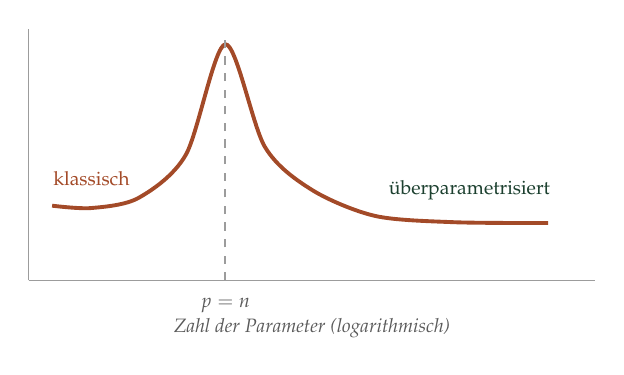
\begin{tikzpicture}[scale=1.0]
\draw[grau!60, line width=0.6pt] (0,0) -- (7.2,0);
\draw[grau!60, line width=0.6pt] (0,0) -- (0,3.2);
\draw[akzent, line width=1.4pt, smooth] plot coordinates {(0.3,0.95) (0.8,0.92) (1.4,1.05) (2.0,1.6) (2.5,3.0) (3.0,1.7) (3.6,1.15) (4.4,0.82) (5.4,0.74) (6.6,0.73)};
\draw[grau!60, line width=0.8pt, dashed] (2.5,0) -- (2.5,3.1);
\node[font=\scriptsize, color=grau, anchor=north] at (2.5,-0.1) {$p = n$};
\node[font=\scriptsize, color=akzent] at (0.8,1.3) {klassisch};
\node[font=\scriptsize, color=gruen!60!black] at (5.6,1.15) {überparametrisiert};
\node[font=\scriptsize\itshape, color=grau] at (3.6,-0.6) {Zahl der Parameter (logarithmisch)};
\end{tikzpicture}
\end{center}

\begin{center}
\begin{minipage}{0.9\textwidth}
\textbf{Genau an der Schwelle $p = n$ explodiert der Fehler. Dahinter fällt er wieder --- und landet unter dem besten klassischen Wert.}
\end{minipage}
\end{center}

\begin{center}
\begin{minipage}{0.88\textwidth}
\kursiv{\textbf{Die U-Kurve aus Kapitel~2 war nur die linke Hälfte des Bildes.} An der Schwelle gibt es genau eine Lösung, die alle Punkte trifft, und sie muss dafür wild ausschlagen --- das ist das Polynom neunten Grades. Jenseits der Schwelle gibt es unendlich viele treffende Lösungen, und man kann die ruhigste davon wählen. Mehr Freiheit erlaubt mehr Ruhe.}
\end{minipage}
\end{center}
\end{merksatz}

\section{Wer wählt die ruhigste Lösung?}

\begin{merksatz}
\boxtitel{Satz 14.1 --- der Gradientenabstieg wählt von selbst}
Seien $p > n$ und $X$ vom Rang $n$. Man minimiere $\|\vek y - X\vek\beta\|^{2}$ durch Gradientenabstieg, beginnend bei $\vek\beta_0 = \vek 0$. Konvergiert das Verfahren gegen eine Lösung mit $X\vek\beta = \vek y$, so ist es diejenige mit der kleinsten Länge:
\[ \vek\beta^{*} = X^{\!\top}(XX^{\!\top})^{-1}\vek y . \]

\schritt{Beweis}
\kursiv{Erstens --- alle Schritte bleiben im Zeilenraum:} Der Gradient ist $-2X^{\!\top}(\vek y - X\vek\beta)$, also ein Vektor der Form $X^{\!\top}\vek c$. Beginnt man bei $\vek 0$ und addiert nur solche Vektoren, so bleibt man im Raum $\{X^{\!\top}\vek c\}$ --- dem Zeilenraum von $X$.

\kursiv{Zweitens --- jede treffende Lösung zerfällt:} Ist $X\vek\beta = \vek y$, so schreibe $\vek\beta = \vek\beta^{*} + \vek v$. Dann ist $X\vek v = \vek y - \vek y = \vek 0$, also liegt $\vek v$ im Kern von $X$.

\kursiv{Drittens --- Kern und Zeilenraum stehen senkrecht:} Für $\vek v$ im Kern und $X^{\!\top}\vek c$ im Zeilenraum gilt $\vek v^{\!\top}X^{\!\top}\vek c = (X\vek v)^{\!\top}\vek c = 0$. Da $\vek\beta^{*}$ im Zeilenraum liegt:
\[ \|\vek\beta\|^{2} = \|\vek\beta^{*}\|^{2} + \|\vek v\|^{2} \ \ge\ \|\vek\beta^{*}\|^{2} . \]

\kursiv{Viertens --- zusammen:} Die treffende Lösung im Zeilenraum hat $\vek v = \vek 0$; das ist $\vek\beta^{*}$, die kürzeste. $\blacksquare$

\begin{center}
\begin{minipage}{0.9\textwidth}
\textbf{Niemand hat eine Strafe hinzugefügt --- und doch wählt das Verfahren die ruhigste aller Lösungen.}
\end{minipage}
\end{center}

\begin{center}
\begin{minipage}{0.88\textwidth}
\kursiv{Das heißt \Begriff{implizite Regularisierung}: Die Strafe steckt nicht in der Zielfunktion, sondern im Verfahren und im Startpunkt. \textbf{Die kürzeste Lösung ist der Grenzfall der Kammregression aus Kapitel~4} für $\lambda \to 0$ --- das Verfahren verhält sich, als hätte es eine unendlich kleine Strafe. Bei der logistischen Regression zeigte Kapitel~5 dasselbe: Dort läuft der Gradientenabstieg zur Trennung mit dem breitesten Rand.}
\end{minipage}
\end{center}

\schritt{Die Grenze des Satzes}
\begin{center}
\begin{minipage}{0.88\textwidth}
\kursiv{Satz 14.1 gilt für lineare Modelle. \textbf{Für tiefe Netze ist nicht bewiesen, welche Lösung der Gradientenabstieg wählt} --- nur, dass er in der Praxis offenbar Lösungen bevorzugt, die gut verallgemeinern. Welche Eigenschaft diese Lösungen gemeinsam haben, ist die zentrale offene Frage der Lerntheorie. Kandidaten sind flache Minima, kleine Normen, geringe Komprimierbarkeit im Sinne von Kapitel~8; keiner erklärt alles.}
\end{minipage}
\end{center}
\end{merksatz}

\section{Warum Tiefe}

\begin{merksatz}
\boxtitel{Satz 14.2 --- was eine Schicht nicht schafft}
Ein Netz mit Gleichrichtern, einem Eingang und einer verdeckten Schicht aus $m$ Einheiten berechnet eine stückweise lineare Funktion mit höchstens $m+1$ Stücken.

\schritt{Beweis}
Jede Einheit $\max\{0,\ w_jx + b_j\}$ hat höchstens einen Knick, bei $x = -b_j/w_j$. Eine gewichtete Summe von $m$ solchen Funktionen hat höchstens $m$ Knicke, also höchstens $m+1$ lineare Stücke. $\blacksquare$
\end{merksatz}

\begin{merksatz}
\boxtitel{Und was Tiefe schafft}
Die \Begriff{Zeltfunktion} auf $[0,1]$:
\[ t(x) = \begin{cases} 2x & x \le \tfrac12\\ 2-2x & x > \tfrac12\end{cases} \ = \ 2\max\{0,x\} - 4\max\{0,\ x-\tfrac12\} \]
--- zwei Gleichrichter.

\schritt{Verkettung}
Wendet man $t$ zweimal an, so entstehen zwei Zelte; dreimal, vier Zelte.

\begin{center}
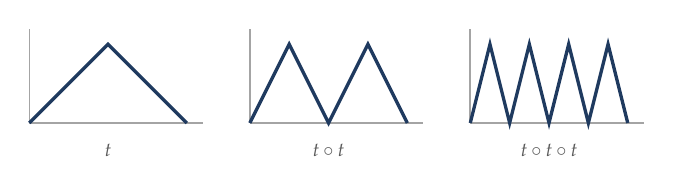
\begin{tikzpicture}[scale=1.0]
\draw[grau!55, line width=0.6pt] (0,0) -- (2.2,0); \draw[grau!55, line width=0.6pt] (0,0) -- (0,1.2);
\draw[tief, line width=1.2pt] (0,0) -- (1,1) -- (2,0);
\node[font=\scriptsize, color=grau] at (1,-0.35) {$t$};
\draw[grau!55, line width=0.6pt] (2.8,0) -- (5.0,0); \draw[grau!55, line width=0.6pt] (2.8,0) -- (2.8,1.2);
\draw[tief, line width=1.2pt] (2.8,0) -- (3.3,1) -- (3.8,0) -- (4.3,1) -- (4.8,0);
\node[font=\scriptsize, color=grau] at (3.8,-0.35) {$t\circ t$};
\draw[grau!55, line width=0.6pt] (5.6,0) -- (7.8,0); \draw[grau!55, line width=0.6pt] (5.6,0) -- (5.6,1.2);
\draw[tief, line width=1.2pt] (5.6,0) -- (5.85,1) -- (6.1,0) -- (6.35,1) -- (6.6,0) -- (6.85,1) -- (7.1,0) -- (7.35,1) -- (7.6,0);
\node[font=\scriptsize, color=grau] at (6.6,-0.35) {$t\circ t\circ t$};
\end{tikzpicture}
\end{center}

\kursiv{Warum sich die Zahl verdoppelt:} $t$ bildet jede der beiden Hälften von $[0,1]$ auf ganz $[0,1]$ ab. Was danach kommt, wird also zweimal durchlaufen --- einmal vorwärts, einmal rückwärts.

\[ t^{L} \ \text{hat}\ 2^{L} \ \text{lineare Stücke.} \]

\begin{center}
{\small
\renewcommand{\arraystretch}{1.5}
\begin{tabular}{@{}P{1.6cm}P{3.0cm}P{3.2cm}@{}}
\toprule
$L$ & \textbf{tief: $L$ Schichten} & \textbf{flach: eine Schicht}\\
\midrule
$5$ & $10$ Einheiten & $\ge 31$ Einheiten\\
$10$ & $20$ Einheiten & $\ge 1023$ Einheiten\\
$20$ & $40$ Einheiten & $\ge 1\,048\,575$ Einheiten\\
\bottomrule
\end{tabular}}
\end{center}

\begin{center}
\begin{minipage}{0.9\textwidth}
\textbf{Was ein tiefes Netz mit vierzig Einheiten berechnet, braucht ein flaches mit über einer Million.}
\end{minipage}
\end{center}

\begin{center}
\begin{minipage}{0.88\textwidth}
\kursiv{\textbf{Tiefe erlaubt Wiederverwendung}: Jede Schicht faltet den Raum, und die nächste arbeitet auf dem gefalteten --- was sie tut, wirkt auf allen Falten zugleich. Ob solche Funktionen in der Medizin vorkommen, ist eine andere Frage. Bei Bildern gibt es gute Gründe dafür: Kanten setzen sich zu Formen zusammen, Formen zu Organen, Organe zu Befunden --- eine Hierarchie, die zu einer Kette von Schichten passt.}
\end{minipage}
\end{center}
\end{merksatz}

\section{Gebaute Annahmen}

\begin{merksatz}
\boxtitel{Architekturen als induktive Neigung}
Satz 1.5 besagte: kein Lernen ohne Annahme. Die erfolgreichen tiefen Netze sind nicht beliebig verschaltet, sondern tragen Annahmen über die Daten in ihrem Aufbau.

\begin{center}
{\small
\renewcommand{\arraystretch}{1.55}
\begin{tabular}{@{}P{2.6cm}P{3.0cm}P{3.0cm}@{}}
\toprule
\textbf{Bauform} & \textbf{Annahme} & \textbf{Anwendung}\\
\midrule
Faltungsnetz & Ein Muster bedeutet an jeder Stelle dasselbe. & Bilder\\
rekurrentes Netz & Die Reihenfolge zählt. & Zeitreihen, Sprache\\
Aufmerksamkeit & Jeder Teil kann sich auf jeden beziehen. & Texte\\
\bottomrule
\end{tabular}}
\end{center}

\begin{center}
\begin{minipage}{0.88\textwidth}
\kursiv{Ein Faltungsnetz benutzt dieselben Gewichte an jeder Stelle des Bildes. \textbf{Ein Rundherd im Röntgenbild sieht oben links so aus wie unten rechts} --- und das Netz muss ihn deshalb nicht an jeder Stelle einzeln lernen. Die Zahl der freien Gewichte sinkt dadurch um Größenordnungen. Das ist dieselbe Einsicht wie beim Merkmal $(T-37)^{2}$ in Kapitel~6: Wer die richtige Annahme einbaut, braucht weniger Daten.}
\end{minipage}
\end{center}
\end{merksatz}

\section{Der Bruchfall}

\begin{warnung}
\boxtitelr{Abkürzungen}
Ein Netz lernt, was in den Daten die Etiketten vorhersagt --- auch wenn es mit der Krankheit nichts zu tun hat.

\begin{center}
{\small
\renewcommand{\arraystretch}{1.52}
\begin{tabular}{@{}P{2.6cm}P{6.0cm}@{}}
\toprule
\textbf{Lungenent\-zündung} & Ein Netz erkannte, aus welcher Klinik ein Röntgenbild stammte --- an Markierungen und Aufnahmetechnik --- und nutzte die unterschiedliche Häufigkeit der Erkrankung in den Kliniken.\\
\textbf{Hautkrebs} & Chirurgische Hautmarkierungen erhöhten die vorhergesagte Melanomwahrscheinlichkeit, weil verdächtige Befunde vor der Aufnahme markiert worden waren.\\
\bottomrule
\end{tabular}}
\end{center}

\begin{center}
\begin{minipage}{0.9\textwidth}
\textbf{In beiden Fällen war die innere Prüfung ausgezeichnet und die äußere schlecht.}
\end{minipage}
\end{center}

\begin{center}
\begin{minipage}{0.88\textwidth}
\kursiv{Das ist das Leck aus Kapitel~3, in einer Form, die man nicht in einer Tabelle von Merkmalen sieht --- es steckt in den Bildpunkten. \textbf{Je mächtiger das Verfahren, desto zuverlässiger findet es solche Abkürzungen}, denn sie sind oft leichter zu lernen als die eigentliche Krankheit. Die erste Warnung des Vorworts gilt hier in ihrer schärfsten Form.}
\end{minipage}
\end{center}
\end{warnung}

\begin{warnung}
\boxtitelr{Unmerkliche Änderungen}
\begin{center}
\begin{minipage}{0.88\textwidth}
\kursiv{Man kann ein Bild so geringfügig verändern, dass kein Mensch einen Unterschied sieht --- und das Netz ordnet es danach völlig anders ein, mit hoher Sicherheit. \textbf{Solche Beispiele gibt es für praktisch jedes tiefe Netz}, und sie lassen sich gezielt berechnen. Sie zeigen, dass die gelernten Merkmale sich von menschlichen Merkmalen grundlegend unterscheiden können, auch wenn beide auf den üblichen Daten zum selben Ergebnis kommen. Nach Kapitel~10 liegt das nahe: In hohen Dimensionen ist jeder Punkt nahe an einer Grenze.}
\end{minipage}
\end{center}
\end{warnung}

\section{Übungsaufgaben}

\begin{aufgabe}
\boxtitel{Aufgabe 14.1 --- Die kürzeste Lösung}
Eine Gleichung, zwei Unbekannte: $\beta_1 + 2\beta_2 = 5$. Bestimmen Sie die kürzeste Lösung und prüfen Sie, dass der Gradientenabstieg von $\vek 0$ aus in ihrer Richtung bleibt.

\loesung
\schritt{Schritt 1 --- Alle Lösungen}
\[ \vek\beta = (5 - 2s,\ s) \quad\text{für jedes } s \]

\schritt{Schritt 2 --- Die kürzeste}
\[ \|\vek\beta\|^{2} = (5-2s)^{2} + s^{2} = 25 - 20s + 5s^{2} \]
\[ \frac{\dd}{\dd s} = -20 + 10s = 0 \quad\Longrightarrow\quad s = 2 \]
\[ \vek\beta^{*} = (1,\ 2), \qquad \|\vek\beta^{*}\| = \sqrt5 = 2{,}236 \]

\schritt{Schritt 3 --- Nach der Formel aus Satz 14.1}
Mit $X = (1\ \ 2)$:
\[ XX^{\!\top} = 1+4 = 5, \qquad \vek\beta^{*} = X^{\!\top}\cdot\tfrac15\cdot5 = (1,\ 2) \quad \checkmark \]

\schritt{Schritt 4 --- Der Gradientenabstieg}
Der Gradient ist $-2\,(5 - \beta_1 - 2\beta_2)\cdot(1,\ 2)$ --- stets ein Vielfaches von $(1,2)$.

\begin{center}
{\small
\renewcommand{\arraystretch}{1.46}
\begin{tabular}{@{}P{1.6cm}P{2.4cm}P{2.4cm}@{}}
\toprule
\textbf{Schritt} & $\vek\beta$ & \textbf{Rest} $5 - \beta_1 - 2\beta_2$\\
\midrule
$0$ & $(0;\ 0)$ & $5$\\
$1$ & $(0{,}5;\ 1{,}0)$ & $2{,}5$\\
$2$ & $(0{,}75;\ 1{,}5)$ & $1{,}25$\\
$\infty$ & $(1;\ 2)$ & $0$\\
\bottomrule
\end{tabular}}
\end{center}
\kursiv{Schrittweite $\eta = 0{,}05$:} $\vek\beta \leftarrow \vek\beta + 0{,}1\cdot\text{Rest}\cdot(1,2)$.

\begin{center}
\begin{minipage}{0.88\textwidth}
\kursiv{\textbf{Jeder Schritt liegt auf der Geraden durch $\vek 0$ in Richtung $(1,2)$}, und die einzige Lösung auf dieser Geraden ist $(1,2)$. Hätte man bei $(5,0)$ begonnen --- auch eine Lösung ---, wäre man dort geblieben. Die implizite Regularisierung hängt also am Startpunkt: Kleine Anfangsgewichte bei Netzen sind aus diesem Grund keine Nebensache.}
\end{minipage}
\end{center}
\end{aufgabe}

\begin{aufgabe}
\boxtitel{Aufgabe 14.2 --- Die Zeltfunktion}
Prüfen Sie $t(x) = 2\max\{0,x\} - 4\max\{0,x-\tfrac12\}$ an drei Stellen und bestimmen Sie $t(t(x))$ bei $x = 0{,}2$ und $x = 0{,}6$.

\loesung
\schritt{Schritt 1 --- Die Darstellung prüfen}
\begin{center}
{\small
\renewcommand{\arraystretch}{1.48}
\begin{tabular}{@{}P{1.4cm}P{2.2cm}P{2.6cm}P{1.8cm}@{}}
\toprule
$x$ & $2\max\{0,x\}$ & $4\max\{0,x-\frac12\}$ & $t(x)$\\
\midrule
$0{,}25$ & $0{,}5$ & $0$ & $0{,}5$\\
$0{,}50$ & $1{,}0$ & $0$ & $1{,}0$\\
$0{,}75$ & $1{,}5$ & $1{,}0$ & $0{,}5$\\
\bottomrule
\end{tabular}}
\end{center}
\kursiv{Probe mit der Definition:} $2\cdot0{,}25 = 0{,}5$; $2\cdot0{,}5 = 1$; $2-2\cdot0{,}75 = 0{,}5$. \checkmark

\schritt{Schritt 2 --- Zweimal anwenden}
\[ x = 0{,}2: \quad t(0{,}2) = 0{,}4, \quad t(0{,}4) = 0{,}8 \]
\[ x = 0{,}6: \quad t(0{,}6) = 0{,}8, \quad t(0{,}8) = 0{,}4 \]

\schritt{Schritt 3 --- Die Stücke von $t\circ t$}
\begin{center}
{\small
\renewcommand{\arraystretch}{1.48}
\begin{tabular}{@{}P{2.4cm}P{2.6cm}@{}}
\toprule
\textbf{Bereich} & $t(t(x))$\\
\midrule
$[0;\ 0{,}25]$ & $4x$\\
$[0{,}25;\ 0{,}5]$ & $2 - 4x$\\
$[0{,}5;\ 0{,}75]$ & $4x - 2$\\
$[0{,}75;\ 1]$ & $4 - 4x$\\
\bottomrule
\end{tabular}}
\end{center}

\kursiv{Probe:} $4\cdot0{,}2 = 0{,}8$ \checkmark; $4\cdot0{,}6-2 = 0{,}4$ \checkmark

\begin{center}
\begin{minipage}{0.88\textwidth}
\kursiv{\textbf{Vier Stücke aus vier Gleichrichtern in zwei Schichten.} Eine Schicht mit vier Einheiten könnte nach Satz 14.2 höchstens fünf Stücke erzeugen --- hier geht es gerade noch gleich auf. Erst bei drei oder mehr Schichten wird der Vorsprung der Tiefe deutlich, wie die Tabelle in Abschnitt 14.4 zeigt.}
\end{minipage}
\end{center}
\end{aufgabe}

\begin{aufgabe}
\boxtitel{Aufgabe 14.3 --- Wo liegt die Schwelle?}
Ein Netz wird an $n$ Patienten trainiert. Bei welcher Größe erwartet man die Spitze des doppelten Abstiegs, und was folgt für die Wahl der Netzgröße?

\loesung
\schritt{Schritt 1 --- Die Schwelle}
Die Spitze liegt dort, wo das Modell gerade eben alle Trainingsdaten treffen kann. Bei linearen Modellen ist das $p = n$.

\schritt{Schritt 2 --- Bei Netzen}
Die Schwelle hängt davon ab, wie viele Parameter nötig sind, um $n$ Punkte auswendig zu lernen. Bei Klassifikation liegt sie etwa bei $p \approx n$ bis $p \approx 2n$.

\begin{center}
{\small
\renewcommand{\arraystretch}{1.48}
\begin{tabular}{@{}P{3.4cm}P{2.4cm}P{2.0cm}@{}}
\toprule
\textbf{Netz aus Kapitel 11} & \textbf{Gewichte} & \textbf{Bereich}\\
\midrule
$4$ Einheiten & $17$ & klassisch\\
$16$ Einheiten & $65$ & klassisch\\
$64$ Einheiten & $257$ & nahe $n$\\
$2\times256$ Einheiten & $66\,817$ & weit darüber\\
\bottomrule
\end{tabular}}
\end{center}
\kursiv{Eine Schicht mit $m$ Einheiten bei zwei Eingängen: $2m + m + m + 1 = 4m+1$ Gewichte; $n = 300$.}

\schritt{Schritt 3 --- Die Folge}
\begin{center}
{\small
\renewcommand{\arraystretch}{1.5}
\begin{tabular}{@{}P{2.6cm}P{6.0cm}@{}}
\toprule
\textbf{klassisch} & Man wählt die Größe durch Kreuzvalidierung, links der Schwelle.\\
\textbf{an der Schwelle} & Die schlechteste Wahl --- das Modell muss alles treffen und hat keine Freiheit, es ruhig zu tun.\\
\textbf{weit darüber} & Oft gut, sofern das Verfahren implizit regularisiert.\\
\bottomrule
\end{tabular}}
\end{center}

\begin{center}
\begin{minipage}{0.88\textwidth}
\kursiv{\textbf{Die gefährlichste Größe ist die mittlere.} Wer ein Netz schrittweise vergrößert und beim ersten Anstieg des Testfehlers aufhört, bleibt vor der Schwelle stehen --- und verpasst womöglich das zweite, tiefere Minimum. Wer es dagegen um einen kleinen Betrag über die Schwelle hinaus vergrößert, erwischt die Spitze. Eine Strafe aus Kapitel~4 glättet die Spitze weitgehend; darum tritt sie in der Praxis selten so scharf auf wie im Versuch.}
\end{minipage}
\end{center}
\end{aufgabe}

\begin{geschichte}
\boxtitelg{Eine Grundsatzdebatte in drei Aufsätzen}
\Person{Chiyuan Zhang}, \Person{Samy Bengio}, \Person{Moritz Hardt}, \Person{Benjamin Recht} und \Person{Oriol Vinyals} veröffentlichten 2017 den Versuch mit vertauschten Etiketten.

\begin{center}
\begin{minipage}{0.9\textwidth}
\kursiv{Der Titel lautete sinngemäß: \enquote{Das Verständnis tiefen Lernens erfordert ein Überdenken der Verallgemeinerung.} \textbf{Er wurde auf der wichtigsten Tagung des Fachs als bester Beitrag ausgezeichnet} --- für einen Befund, der keine neue Methode enthielt, sondern zeigte, dass die vorhandene Theorie nicht ausreicht.}
\end{minipage}
\end{center}

\schritt{Der doppelte Abstieg}
\Person{Mikhail Belkin}, \Person{Daniel Hsu}, \Person{Siyuan Ma} und \Person{Soumik Mandal} beschrieben 2019 die Kurve aus Abschnitt 14.2 und gaben ihr den Namen.

\begin{center}
\begin{minipage}{0.9\textwidth}
\kursiv{Spätere Nachforschungen fanden die Spitze an der Interpolationsschwelle schon in Arbeiten aus den 1990er Jahren, zu linearen Modellen und kleinen Netzen. \textbf{Sie war beobachtet, aber als Merkwürdigkeit abgetan worden}, weil die Theorie sagte, jenseits der Schwelle könne es nur schlechter werden. Niemand hatte weiter gerechnet.}
\end{minipage}
\end{center}

\schritt{Die Tiefe}
\begin{center}
\begin{minipage}{0.9\textwidth}
\kursiv{\Person{Matus Telgarsky} bewies 2016 mit der Zeltfunktion, dass bestimmte Funktionen mit tiefen Netzen exponentiell sparsamer darstellbar sind als mit flachen. \textbf{Der Beweis ist kaum länger als Aufgabe 14.2} --- einer der seltenen Fälle, in denen ein tiefes Ergebnis der Lerntheorie mit elementaren Mitteln auskommt.}
\end{minipage}
\end{center}
\end{geschichte}

\begin{forschung}
\boxtitelp{Die offene Frage}
\begin{center}
{\small
\renewcommand{\arraystretch}{1.45}
\begin{tabular}{@{}P{2.8cm}P{5.4cm}@{}}
\toprule
\textbf{Gutartige Überanpassung} & Wann das Treffen verrauschter Daten nicht schadet --- für lineare Modelle inzwischen genau beschrieben.\\
\textbf{Flache Minima} & Ob breite Täler besser verallgemeinern als enge --- umstritten.\\
\textbf{Skalengesetze} & Der Testfehler fällt mit Daten und Parametern nach einem Potenzgesetz.\\
\bottomrule
\end{tabular}}
\end{center}

\schritt{Zur dritten Zeile}
\begin{center}
\begin{minipage}{0.88\textwidth}
\kursiv{Seit 2020 wurde bei großen Sprachmodellen beobachtet, dass der Fehler über viele Größenordnungen als Potenz der Datenmenge und der Parameterzahl fällt --- ohne erkennbare Sättigung. \textbf{Diese Gesetze sind empirisch, nicht bewiesen}, und sie haben die Entwicklung des Fachs stärker gesteuert als jeder Satz dieses Bandes: Sie rechtfertigten Investitionen in immer größere Modelle. Warum sie gelten und wo sie enden, ist unbekannt.}
\end{minipage}
\end{center}
\end{forschung}

\begin{merksatz}
\boxtitel{Was Sie jetzt können}
\begin{center}
\renewcommand{\arraystretch}{1.5}
\begin{tabular}{@{}P{3.0cm}P{5.6cm}@{}}
\toprule
\textbf{Der Versuch} & dasselbe Netz lernt Sinn und Unsinn\\
\textbf{Doppelter Abstieg} & Spitze bei $p = n$, zweites Tal dahinter\\
\textbf{Satz 14.1} & Gradient von $\vek 0$ wählt die kürzeste Lösung\\
\textbf{Satz 14.2} & eine Schicht: $m+1$ Stücke; $L$ Schichten: $2^{L}$\\
\textbf{Der Bruchfall} & Abkürzungen statt Krankheit\\
\bottomrule
\end{tabular}
\end{center}

\begin{center}
\begin{minipage}{0.88\textwidth}
\kursiv{Damit endet Teil~V. Das letzte Kapitel zieht Bilanz --- und kehrt zum Sepsis-System von 2021 zurück, um zu fragen, welche der Werkzeuge dieses Bandes seinen Fehlschlag hätten verhindern können.}
\end{minipage}
\end{center}
\end{merksatz}

\part{Aktueller Stand}

\chapter{Was sich verallgemeinern lässt}

\section{Zurück zum Fall von 2021}

\begin{merksatz}
\boxtitel{Hätte dieser Band den Fehlschlag verhindert?}
Das Sepsis-Warnsystem, das 2021 an einer unabhängigen Klinik nachgeprüft wurde, warnte bei fast jedem fünften Patienten und übersah zwei Drittel der Sepsisfälle. Die Trennschärfe fiel von angegebenen $0{,}76$ bis $0{,}83$ auf $0{,}63$.\zit{26}

\begin{center}
{\small
\renewcommand{\arraystretch}{1.52}
\begin{tabular}{@{}P{1.2cm}P{3.4cm}P{4.0cm}@{}}
\toprule
\textbf{Kap.} & \textbf{Werkzeug} & \textbf{Was es gezeigt hätte}\\
\midrule
$1$ & Prävalenz und Kosten & Die Schwelle passt nicht zur neuen Klinik.\\
$3$ & äußere Prüfung & Die Trennschärfe gilt nur für die eigenen Daten.\\
$3$ & zeitliches Leck & Welche Merkmale erst nach dem Verdacht vorliegen.\\
$5$, $11$ & Kalibrierung & Ob $30$ Prozent wirklich $30$ Prozent heißt.\\
$12$ & Etiketten & Welche Definition von Sepsis gelernt wurde.\\
\midrule
$7$, $8$ & Schranken & \textcolor{akzent}{nichts}\\
\bottomrule
\end{tabular}}
\end{center}

\begin{center}
\begin{minipage}{0.9\textwidth}
\textbf{Die Werkzeuge, die geholfen hätten, sind die unscheinbaren. Die Theorie der Verallgemeinerung hätte nicht geholfen.}
\end{minipage}
\end{center}

\begin{center}
\begin{minipage}{0.88\textwidth}
\kursiv{Die Sätze aus Teil~III beschreiben die Übertragung auf neue Patienten \kursiv{derselben Verteilung}. \textbf{Das Problem von 2021 war eine andere Verteilung} --- andere Klinik, andere Praxis, andere Etiketten. Dafür gibt es keine Schranke, sondern nur Sorgfalt: die Prüfung an fremden Daten, bevor man ein Verfahren einsetzt, und die fortlaufende Beobachtung danach.}
\end{minipage}
\end{center}
\end{merksatz}

\section{Vier Muster}

\begin{merksatz}
\boxtitel{Muster 1 --- ohne Annahme kein Lernen}
\begin{center}
{\small
\renewcommand{\arraystretch}{1.48}
\begin{tabular}{@{}P{1.4cm}P{7.0cm}@{}}
\toprule
$1$ & Satz 1.5: Über alle denkbaren Welten gemittelt sind alle Verfahren gleich.\\
$6$ & Das Merkmal $(T-37)^{2}$ schlägt den Kern --- weil es Wissen enthält.\\
$10$ & Das Abstandsmaß ist das ganze Modell.\\
$14$ & Faltungsnetze tragen die Annahme, dass Muster überall dasselbe bedeuten.\\
\bottomrule
\end{tabular}}
\end{center}

\begin{center}
\begin{minipage}{0.88\textwidth}
\kursiv{\textbf{Jedes erfolgreiche Verfahren dieses Bandes hat eine Annahme, die zur Aufgabe passt.} Die Kunst liegt darin, sie zu erkennen --- und wer sie kennt, sollte sie hineinstecken, statt sie suchen zu lassen.}
\end{minipage}
\end{center}
\end{merksatz}

\begin{merksatz}
\boxtitel{Muster 2 --- weniger Freiheit, bis zur Schwelle}
\begin{center}
{\small
\renewcommand{\arraystretch}{1.48}
\begin{tabular}{@{}P{1.4cm}P{7.0cm}@{}}
\toprule
$2$ & Optimismus $2\sigma^{2}p/n$: jeder Parameter kostet.\\
$4$ & Strafen senken den vermeidbaren Fehler auf ein Drittel.\\
$7$ & Die VC-Dimension bestimmt den Datenbedarf.\\
$8$ & Breiter Rand, wenige Stützvektoren, kurze Beschreibung.\\
$14$ & \textcolor{akzent}{Und jenseits der Schwelle gilt es nicht mehr.}\\
\bottomrule
\end{tabular}}
\end{center}

\begin{center}
\begin{minipage}{0.88\textwidth}
\kursiv{Die ersten vier Zeilen sind ein zusammenhängendes, bewiesenes Lehrgebäude. \textbf{Die fünfte stellt es nicht in Frage, sondern zeigt seine Grenze}: Es beschreibt die Klasse der Regeln, nicht das Verfahren, das darin sucht. Sobald das Verfahren selbst regularisiert --- wie der Gradientenabstieg in Satz 14.1 ---, zählt nicht mehr, wie viele Regeln es gibt, sondern welche gefunden wird.}
\end{minipage}
\end{center}
\end{merksatz}

\begin{merksatz}
\boxtitel{Muster 3 --- die Prüfung ist wichtiger als das Verfahren}
\begin{center}
{\small
\renewcommand{\arraystretch}{1.48}
\begin{tabular}{@{}P{1.4cm}P{7.0cm}@{}}
\toprule
$3$ & Ein Leck macht aus Rauschen $98{,}5$ Prozent Treffsicherheit.\\
$3$ & Zwanzig verglichene Modelle täuschen fünf Prozentpunkte vor.\\
$8$ & Die Schranken ordnen, aber messen nicht; die Kreuzvalidierung misst.\\
$14$ & Abkürzungen fallen erst an fremden Daten auf.\\
\bottomrule
\end{tabular}}
\end{center}

\begin{center}
\begin{minipage}{0.88\textwidth}
\kursiv{\textbf{Der Unterschied zwischen einem guten und einem schlechten Verfahren ist meist kleiner als der zwischen einer ehrlichen und einer fehlerhaften Prüfung.} Eine Übersicht über $71$ klinische Studien fand bei fairem Vergleich keinen Vorteil lernender Verfahren gegenüber der logistischen Regression\zit{5} --- aber reichlich Fälle, in denen die Prüfung den Unterschied erzeugt hatte.}
\end{minipage}
\end{center}
\end{merksatz}

\begin{merksatz}
\boxtitel{Muster 4 --- Vorhersage ist nicht Erklärung}
\begin{center}
{\small
\renewcommand{\arraystretch}{1.48}
\begin{tabular}{@{}P{1.4cm}P{7.0cm}@{}}
\toprule
$4$ & Das Lasso wählt falsche Merkmale in jedem fünften Fall.\\
$9$ & Ein Zufallsmerkmal steht in jedem fünften Baum an zweiter Stelle.\\
$12$ & Gruppen entstehen auch aus Gleichverteilung.\\
$13$ & Die Richtung größter Streuung kann bedeutungslos sein.\\
\bottomrule
\end{tabular}}
\end{center}

\begin{center}
\begin{minipage}{0.88\textwidth}
\kursiv{\textbf{Ein Verfahren, das gut vorhersagt, hat nicht verstanden, warum.} Die Merkmale, die es benutzt, die Gruppen, die es bildet, die Richtungen, die es findet --- sie beschreiben die Daten, nicht die Krankheit. Wer aus ihnen Mechanismen ableitet, verlässt die Mathematik dieses Bandes und braucht eine andere: die der Ursachen, die hier nicht behandelt wurde.}
\end{minipage}
\end{center}
\end{merksatz}

\section{Was offen ist}

\begin{merksatz}
\boxtitel{Vier Fragen}
\begin{center}
{\small
\renewcommand{\arraystretch}{1.55}
\begin{tabular}{@{}P{3.2cm}P{5.4cm}@{}}
\toprule
\textbf{Verallgemei\-nerung} & Warum lernen überparametrisierte Netze? Kapitel~14 zeigt Teilantworten, keine vollständige.\\
\textbf{Übertragung} & Wann gilt, was an einer Klinik gelernt wurde, auch an einer anderen?\\
\textbf{Ursachen} & Welche Behandlung hilft diesem Patienten? Vorhersage beantwortet das nicht.\\
\textbf{Gerechtigkeit} & Wie verhindert man, dass ein Verfahren bestehende Ungleichheit fortschreibt?\\
\bottomrule
\end{tabular}}
\end{center}
\end{merksatz}

\begin{warnung}
\boxtitelr{Zur vierten Frage: ein Fall aus dem Jahr 2019}
Ein in amerikanischen Kliniken weit verbreitetes Verfahren sollte Patienten mit hohem Betreuungsbedarf erkennen. Gelernt hatte es aus den \kursiv{Behandlungskosten} der Vorjahre.\zit{16}

\begin{center}
\begin{minipage}{0.88\textwidth}
\kursiv{Weil schwarze Patienten bei gleicher Krankheitslast im Durchschnitt weniger Behandlung erhalten hatten --- aus Gründen des Zugangs, nicht des Bedarfs ---, waren ihre Kosten niedriger. \textbf{Das Verfahren sagte die Kosten richtig vorher und den Bedarf falsch}: Bei gleicher Risikoeinstufung waren schwarze Patienten deutlich kränker. Nach Berichtigung der Zielgröße hätte sich der Anteil schwarzer Patienten im Förderprogramm mehr als verdoppelt.}
\end{minipage}
\end{center}

\begin{center}
\begin{minipage}{0.9\textwidth}
\textbf{Kein Fehler im Verfahren --- ein Fehler in der Wahl dessen, was es lernen sollte.}
\end{minipage}
\end{center}

\begin{center}
\begin{minipage}{0.88\textwidth}
\kursiv{Das ist die erste Warnung des Vorworts in ihrer folgenreichsten Gestalt. \textbf{Ein Verfahren lernt, was in den Daten steht}, und wenn in den Daten eine Ungerechtigkeit steht, lernt es die Ungerechtigkeit --- mit derselben Zuverlässigkeit, mit der es alles andere lernt. Die Mathematik kann das nicht bemerken. Es bemerken nur Menschen, die wissen, wie die Daten entstanden sind.}
\end{minipage}
\end{center}
\end{warnung}

\section{Sechs Sätze, die bleiben}

\begin{merksatz}
\boxtitel{Die Bilanz}
\begin{center}
{\small
\renewcommand{\arraystretch}{1.55}
\begin{tabular}{@{}P{0.7cm}P{7.7cm}@{}}
\toprule
$1$ & Die beste Regel entscheidet überall für das Wahrscheinlichere --- und kein Verfahren unterbietet ihren Fehler, solange es nur dieselben Merkmale kennt.\\
$2$ & Der Fehler auf neuen Daten besteht aus Rauschen, Verzerrung und Varianz; nur die letzten beiden hängen vom Verfahren ab.\\
$3$ & Alles, was aus den Daten gelernt wird, gehört in die Prüfung, nicht davor.\\
$4$ & Eine Klasse ist genau dann lernbar, wenn ihre VC-Dimension endlich ist.\\
$5$ & Mitteln hilft nur so weit, wie die Gemittelten sich unterscheiden.\\
$6$ & Der Gradientenabstieg von null wählt unter allen passenden Lösungen die kürzeste.\\
\bottomrule
\end{tabular}}
\end{center}
\end{merksatz}

\begin{merksatz}
\boxtitel{Ein Schlusswort}
\begin{center}
\begin{minipage}{0.9\textwidth}
Dieser Band begann mit einer Frage, die älter ist als jedes Verfahren: Wie gewinnt man aus hundert Beobachtungen eine Regel, die auch für die hunderterste stimmt?

Vierzehn Kapitel später lässt sich sagen, was das Fach darauf antwortet. Es antwortet nicht mit einem Verfahren, sondern mit einer Rechnung: wie viele Beobachtungen man braucht, wenn man wenig Freiheit lässt; wie man die Freiheit misst; woran man merkt, dass man zu viel gelassen hat. Und es antwortet mit einer Warnung: dass jede dieser Rechnungen voraussetzt, die hunderterste Beobachtung stamme aus derselben Welt wie die ersten hundert.

In der Klinik tut sie das selten. Patienten wechseln, Praxis ändert sich, Definitionen werden neu gefasst. Das Lernen aus Daten ist darum nicht das Ende des ärztlichen Urteils, sondern eine seiner Voraussetzungen --- eine Rechnung, die man kennen muss, um zu wissen, wann man ihr nicht trauen darf.
\end{minipage}
\end{center}

\begin{center}
\begin{minipage}{0.88\textwidth}
\kursiv{Damit steht dieser Band neben den vorangegangenen. Die Statistik sagt, was die Daten hergeben. Die Optimierung sagt, was es kostet. Die Informationstheorie sagt, was übertragbar ist. Die Spieltheorie sagt, was übrig bleibt, wenn der andere es auch weiß. \textbf{Und das Lernen sagt, was von alldem auf den nächsten Fall zutrifft --- und wann nicht.}}
\end{minipage}
\end{center}
\end{merksatz}

\appendix
\part{Anhang}

\newcommand{\lit}[3]{\vspace{5pt}\noindent\textbf{[#1]} #2\par\nopagebreak\vspace{1pt}{\small\itshape\color{grau} #3}\par\vspace{2pt}}

\chapter{Formelsammlung und Übersicht}

\section{Das Problem}

\begin{merksatz}
\boxtitel{Teil I}
\begin{center}
{\small
\renewcommand{\arraystretch}{1.62}
\begin{tabular}{@{}P{4.4cm}P{4.2cm}@{}}
\toprule
$\Risk(h) = \E[L(h(X),Y)]$ & Risiko (1.2)\\
$h^{*}(x) = [\eta(x) \ge \tfrac12]$ & Bayes-Regel (1.3)\\
$\eta \ge c_{\text{FP}}/(c_{\text{FP}}+c_{\text{FN}})$ & mit Kosten\\
kein Verfahren überall besser & Satz 1.5\\
$\sigma^{2} + \text{Verzerrung}^{2} + \text{Varianz}$ & Satz 2.1\\
$2\sigma^{2}p/n$ & Optimismus (2.2)\\
$c^{*} = \mu^{2}/(\mu^{2}+\sigma^{2})$ & Schrumpfen\\
$e_i/(1-H_{ii})$ & Weglassen (3.2)\\
Anteil richtig geordneter Paare & Trennschärfe (3.3)\\
$\sqrt{2\ln m/n}$ & höchste Zufallskorrelation\\
\bottomrule
\end{tabular}}
\end{center}
\end{merksatz}

\section{Die Verfahren}

\begin{merksatz}
\boxtitel{Teil II und IV}
\begin{center}
{\small
\renewcommand{\arraystretch}{1.62}
\begin{tabular}{@{}P{4.4cm}P{4.2cm}@{}}
\toprule
$1/(1-\rho^{2})$ & Kollinearität\\
$(X^{\!\top}X+\lambda I)^{-1}X^{\!\top}\vek y$ & Kamm (4.2)\\
$d_j^{2}/(d_j^{2}+\lambda)$ & Schrumpffaktor\\
$\operatorname{sign}(b)(|b|-\lambda)_{+}$ & Lasso (4.4)\\
$\ln\frac{p}{1-p} = \beta_0 + \vek\beta^{\!\top}\vek x$ & logistisch (5.1)\\
$\nabla J = \sum(p_i-y_i)\vek x_i$ & Gradient (5.2)\\
$(R/\gamma)^{2}$ & Perzeptron (5.3)\\
$\vek w = \sum\alpha_i t_i\vek x_i$ & Stützvektoren (6.2)\\
$e^{-\gamma\|\vek x-\vek z\|^{2}}$ & Gauß-Kern\\
$-p\log_2p - (1-p)\log_2(1-p)$ & Entropie (9.1)\\
$\rho\sigma^{2} + (1-\rho)\sigma^{2}/B$ & Mittel (9.2)\\
$\prod 2\sqrt{\varepsilon_s(1-\varepsilon_s)}$ & Boosting (9.3)\\
$2\Risk^{*}(1-\Risk^{*})$ & ein Nachbar (10.2)\\
$e = r^{1/p}$ & Kantenlänge\\
$\sigma(1-\sigma) \le \tfrac14$ & verschwindender Gradient\\
\bottomrule
\end{tabular}}
\end{center}
\end{merksatz}

\section{Theorie und Tiefe}

\begin{merksatz}
\boxtitel{Teil III und V}
\begin{center}
{\small
\renewcommand{\arraystretch}{1.62}
\begin{tabular}{@{}P{4.4cm}P{4.2cm}@{}}
\toprule
$(\ln|\Hyp| + \ln\frac1\delta)/\varepsilon$ & fehlerfrei (7.2)\\
$(\ln|\Hyp| + \ln\frac2\delta)/(2\varepsilon^{2})$ & allgemein (7.3)\\
$2e^{-2n\varepsilon^{2}}$ & Hoeffding\\
$\sum_{i\le d}\binom ni \le (en/d)^{d}$ & Sauer (7.5)\\
$\hat\Risk + \sqrt{\frac8n(d\ln\frac{2en}{d}+\ln\frac4\delta)}$ & VC (7.6)\\
Stützvektoren$/n$ & Weglassen (8.1)\\
$(k\ln n + \ln\frac1\delta)/(n-k)$ & Kompression (8.2)\\
$d \le (R/\gamma)^{2}$ & Rand (8.3)\\
$\sum_j\sum_{C_j}\|\vek x_i-\vek\mu_j\|^{2}$ & $k$-Mittel (12.1)\\
$\max\vek u^{\!\top}\Sigma\vek u = \lambda_1$ & Hauptkomp.\ (13.1)\\
$1+\rho(p-1)$ und $1-\rho$ & gleiche Verbundenheit\\
$X^{\!\top}(XX^{\!\top})^{-1}\vek y$ & kürzeste Lösung (14.1)\\
$m+1$ gegen $2^{L}$ Stücke & Tiefe (14.2)\\
\bottomrule
\end{tabular}}
\end{center}
\end{merksatz}

\section{Was in diesem Band \kursiv{nicht} bewiesen wurde}

\begin{merksatz}
\boxtitel{Neun Auslassungen}
\begin{center}
{\small
\renewcommand{\arraystretch}{1.5}
\begin{tabular}{@{}P{3.6cm}P{1.2cm}P{3.2cm}@{}}
\toprule
\textbf{Ergebnis} & \textbf{Kap.} & \textbf{Wo es steht}\\
\midrule
Weglassformel & $3$ & Hastie u.\,a.\zit{11}, Kap.\ 7\\
Satz von Mercer & $6$ & Schölkopf, Smola\zit{22}\\
Hoeffding & $7$ & Shalev-Shwartz\zit{24}, Anh.\ B\\
Sauer & $7$ & Shalev-Shwartz\zit{24}, Kap.\ 6\\
Fundamentalsatz (VC) & $7$ & Shalev-Shwartz\zit{24}, Kap.\ 28\\
Grenzübergang Nachbar & $10$ & Cover, Hart\zit{6}\\
Universelle Näherung & $11$ & Goodfellow u.\,a.\zit{10}\\
EM-Monotonie & $12$ & Bishop\zit{3}, Kap.\ 9\\
Eckart-Young & $13$ & Deisenroth u.\,a.\zit{7}\\
\bottomrule
\end{tabular}}
\end{center}

\begin{center}
\begin{minipage}{0.88\textwidth}
\kursiv{Neun Auslassungen, jede im Text benannt, mit Begründung und Fundstelle. \textbf{Alle übrigen Sätze des Bandes sind vollständig bewiesen} --- darunter die Kompressionsschranke, die Randdimension über das Perzeptron, AdaBoost, die Schranke über Stützvektoren und die kürzeste Lösung des Gradientenabstiegs.}
\end{minipage}
\end{center}
\end{merksatz}

\section{Die Landkarte des Bandes}

\begin{merksatz}
\boxtitel{Welcher Satz worauf beruht}
\begin{center}
{\small
\renewcommand{\arraystretch}{1.4}
\begin{tabular}{@{}P{3.4cm}P{1.0cm}P{3.8cm}@{}}
\toprule
\textbf{Ergebnis} & \textbf{Kap.} & \textbf{beruht auf}\\
\midrule
Bayes-Regel & $1$ & punktweise Minimierung\\
Zerlegung & $2$ & Quadrieren, Erwartungswert\\
Optimismus & $2$ & Spur einer Projektion\\
Kamm & $4$ & positiv definite Matrix\\
Lasso & $4$ & Fallunterscheidung am Knick\\
Konvexität & $5$ & $\sigma' = \sigma(1-\sigma)$\\
Perzeptron & $5$ & Cauchy-Schwarz\\
Stützvektoren & $6$ & komplementärer Schlupf (Band 19)\\
endliche Klassen & $7$ & Vereinigung, $1-\varepsilon \le e^{-\varepsilon}$\\
Weglassen & $8$ & komplementärer Schlupf\\
Kompression & $8$ & wie Satz 7.2\\
Randdimension & $8$ & Perzeptron, Satz 5.3\\
Mittel & $9$ & Kovarianzen summieren\\
Boosting & $9$ & Exponent über Indikator\\
ein Nachbar & $10$ & Varianz $\ge 0$\\
$k$-Mittel & $12$ & Durchschnitt minimiert\\
Hauptkomponenten & $13$ & Spektralsatz (Band 2)\\
kürzeste Lösung & $14$ & Zeilenraum $\perp$ Kern\\
Tiefe & $14$ & Knicke zählen\\
\bottomrule
\end{tabular}}
\end{center}
\end{merksatz}

\section{Zeittafel}

\begin{merksatz}
\boxtitel{Von Hume bis zu den Skalengesetzen}
\begin{center}
{\small
\renewcommand{\arraystretch}{1.32}
\begin{tabular}{@{}P{1.3cm}P{3.0cm}P{4.0cm}@{}}
\toprule
\textbf{Jahr} & \textbf{Person} & \textbf{Ereignis}\\
\midrule
$1739$ & Hume & das Induktionsproblem\\
$1838$ & Verhulst & die logistische Kurve\\
$1894$ & Pearson & Mischung zweier Krabbenarten\\
$1901$ & Pearson & erste Hauptkomponente\\
$1904$ & Spearman & der allgemeine Faktor\\
$1933$ & Hotelling & Hauptkomponenten als Eigenwerte\\
$1936$ & Fisher & Diskriminanzanalyse\\
$1936$ & Eckart, Young & beste Näherung\\
$1943$ & Tichonow & Regularisierung\\
$1950$ & Turing & lernende Maschinen\\
$1951$ & Fix, Hodges & nächste Nachbarn\\
$1956$ & Stein & das Paradoxon\\
$1957$ & Bellman & Fluch der Dimension\\
$1957$ & Lloyd & $k$ Mittelpunkte\\
$1958$ & Rosenblatt & das Perzeptron\\
$1959$ & Samuel & der Name\\
$1962$ & Novikoff & Konvergenz des Perzeptrons\\
$1963$ & Vapnik, Tscherwonenkis & breitester Rand\\
$1967$ & Cover, Hart & ein Nachbar, doppeltes Risiko\\
$1969$ & Minsky, Papert & \kursiv{Perceptrons}\\
$1970$ & Hoerl, Kennard & Kammregression\\
$1971$ & \textbf{Vapnik, Tscherwonenkis} & \textbf{VC-Dimension}\\
$1972$ & Sauer, Shelah & das Lemma\\
$1974$ & Stone & Kreuzvalidierung\\
$1977$ & Dempster, Laird, Rubin & EM\\
$1984$ & Valiant & PAC-Lernen\\
$1984$ & Breiman u.\,a. & Entscheidungsbäume\\
$1986$ & Rumelhart, Hinton, Williams & Rückpropagation\\
$1986$ & Littlestone, Warmuth & Kompression\\
$1989$ & Cybenko & universelle Näherung\\
$1992$ & Boser, Guyon, Vapnik & Kerntrick\\
$1995$ & Freund, Schapire & AdaBoost\\
$1996$ & Tibshirani & Lasso\\
$2001$ & Breiman & Zufallswald, zwei Kulturen\\
$2002$ & Ambroise, McLachlan & das Leck\\
$2012$ & Krizhevsky u.\,a. & tiefe Netze gewinnen\\
$2016$ & Telgarsky & Tiefe\\
$2017$ & \textbf{Zhang u.\,a.} & \textbf{vertauschte Etiketten}\\
$2019$ & Belkin u.\,a. & doppelter Abstieg\\
$2019$ & Obermeyer u.\,a. & Kosten statt Bedarf\\
$2019$ & Seymour u.\,a. & Sepsis-Phänotypen\\
$2020$ & --- & Skalengesetze\\
$2021$ & Wong u.\,a. & Nachprüfung des Sepsissystems\\
$2023$ & Kapoor, Narayanan & Lecks in $17$ Fächern\\
\bottomrule
\end{tabular}}
\end{center}
\end{merksatz}

\section{Glossar}

\begin{merksatz}
\boxtitel{Begriffe von A bis Z}
\begin{center}
{\small
\renewcommand{\arraystretch}{1.3}
\begin{longtable}{@{}P{3.6cm}P{5.0cm}@{}}
\toprule
\textbf{Begriff} & \textbf{Bedeutung}\\
\midrule
\endhead
Äußere Prüfung & an Daten einer anderen Klinik (3)\\
Bagging & Mittel über Neuziehungen (9)\\
Bayes-Regel & überall das Wahrscheinlichere (1.3)\\
Bayes-Risiko & kleinstmöglicher Fehler (1)\\
Doppelter Abstieg & zweites Tal jenseits $p = n$ (14)\\
EM-Verfahren & Erwartung, Maximierung (12)\\
Ersatzverlust & konvexe Näherung an Null-Eins (6)\\
Gauß-Kern & Ähnlichkeit über Abstand (6)\\
Hauptkomponente & Richtung größter Streuung (13)\\
Implizite Regularisierung & Strafe im Verfahren, nicht im Ziel (14)\\
Induktive Neigung & eingebaute Annahme (1)\\
Kalibrierung & $30\,\%$ heißt $30\,\%$ (3)\\
Kammregression & Strafe $\lambda\|\vek\beta\|^{2}$ (4.1)\\
Kern & Skalarprodukt im Merkmalsraum (6.3)\\
Kompression & Regel aus $k$ Punkten (8)\\
Kreuzvalidierung & reihum zurückhalten (3.1)\\
Kreuzentropie & Verlust der log.\ Regression (5)\\
Lasso & Strafe $\lambda\|\vek\beta\|_1$ (4.3)\\
Leck & Information aus der Prüfung im Lernen (3)\\
Nächste Nachbarn & Mehrheit der ähnlichsten (10.1)\\
Optimismus & Test minus Training (2.2)\\
PAC & wahrscheinlich ungefähr richtig (7.1)\\
Perzeptron & Korrektur bei Fehler (5)\\
Rand & Abstand zur Grenze (6.1)\\
Risiko & erwarteter Verlust (1.2)\\
Rückpropagation & Kettenregel rückwärts (11)\\
Stützvektor & Punkt auf dem Rand (6.2)\\
Trennschärfe & Paarvergleich, AUC (3.3)\\
Überanpassung & Varianz überwiegt (2)\\
Unteranpassung & Verzerrung überwiegt (2)\\
VC-Dimension & größte zerschmetterte Menge (7.4)\\
Verzerrung & mittlere Abweichung (2)\\
Zerschmettern & jede Einteilung erreichen (7.4)\\
Zufallswald & Bäume mit Zufallsauswahl (9)\\
\bottomrule
\end{longtable}}
\end{center}
\end{merksatz}

\chapter{Kommentierte Quellen}

Achtundzwanzig Werke, eingeordnet: Zu jedem steht, wofür man es aufschlägt und was es leistet, das andere nicht leisten.

\lit{1}{Abu-Mostafa, Y., Magdon-Ismail, M., Lin, H.-T.: \textit{Learning From Data}. AMLBook 2012.}{Kurz, klar und auf die Kernfrage dieses Bandes ausgerichtet: Wann ist Lernen überhaupt möglich? Die VC-Theorie wird hier so zugänglich erklärt wie nirgends sonst. Etwa zweihundert Seiten; die beste Brücke zwischen Teil~I und Teil~III.}

\lit{2}{Belkin, M., Hsu, D., Ma, S., Mandal, S.: \textit{Reconciling modern machine-learning practice and the classical bias--variance trade-off}. PNAS 116, 2019.}{Der Aufsatz, der den doppelten Abstieg benannte. Zeigt die Kurve aus Kapitel~14 an linearen Modellen, Zufallsmerkmalen und Netzen. Kurz und für Nichtfachleute lesbar.}

\lit{3}{Bishop, C.: \textit{Pattern Recognition and Machine Learning}. Springer 2006.}{Das Lehrbuch aus wahrscheinlichkeitstheoretischer Sicht. Mischmodelle und EM (Kapitel~9), Kerne und Gaußprozesse sind besonders gut dargestellt. Anspruchsvoll, mit vielen Abbildungen; die Fundstelle für die achte Auslassung.}

\lit{4}{Breiman, L.: \textit{Statistical Modeling: The Two Cultures}. Statistical Science 16, 2001.}{\textbf{Der Streitaufsatz, der das Verhältnis von Statistik und Lernen neu bestimmte.} Breiman wirft der Statistik vor, an Modellen festzuhalten, wo Vorhersagegüte zählt. Die angehängten Erwiderungen --- unter anderem von Cox und Efron --- sind ebenso lesenswert wie der Aufsatz selbst.}

\lit{5}{Christodoulou, E. u.\,a.: \textit{A systematic review shows no performance benefit of machine learning over logistic regression for clinical prediction models}. J.\ Clin.\ Epidemiol.\ 110, 2019.}{Die Übersicht über $71$ Vergleichsstudien aus Kapitel~5 und 15. Unverzichtbar für jeden, der ein lernendes Verfahren in der Klinik einsetzen will: Sie zeigt, wie oft der scheinbare Vorteil aus der Prüfung stammt.}

\lit{6}{Cover, T., Hart, P.: \textit{Nearest neighbor pattern classification}. IEEE Trans.\ Inf.\ Theory 13, 1967.}{Die Originalarbeit zu Satz 10.2, sieben Seiten. Enthält den Grenzübergang, den Kapitel~10 ausließ, und die Formulierung, dass die Hälfte der Information im nächsten Nachbarn steckt.}

\lit{7}{Deisenroth, M., Faisal, A., Ong, C.: \textit{Mathematics for Machine Learning}. Cambridge 2020.}{Die mathematischen Werkzeuge des Faches --- lineare Algebra, Analysis, Wahrscheinlichkeit, Optimierung --- auf das Lernen zugeschnitten. Für Leser, die Band 2 und 19 nicht zur Hand haben. Frei verfügbar; die Fundstelle für Eckart-Young.}

\lit{8}{Ertel, W.: \textit{Grundkurs Künstliche Intelligenz}. 5.\ Aufl., Springer Vieweg 2021.}{\textbf{Auf Deutsch, als Überblick.} Behandelt maschinelles Lernen im Rahmen der künstlichen Intelligenz insgesamt, mit Logik, Suche und Schließen. Gut lesbar, mit vielen Übungen; weniger Tiefe in der Theorie als die englischen Lehrbücher.}

\lit{9}{Frochte, J.: \textit{Maschinelles Lernen --- Grundlagen und Algorithmen in Python}. 3.\ Aufl., Hanser 2020.}{\textbf{Auf Deutsch und praktisch.} Die Verfahren dieses Bandes mit lauffähigem Code, von der Regression bis zu Netzen. Für Leser, die das Gelesene selbst ausprobieren wollen.}

\lit{10}{Goodfellow, I., Bengio, Y., Courville, A.: \textit{Deep Learning}. MIT Press 2016.}{Das Standardwerk zu tiefen Netzen, von dreien, die das Gebiet geprägt haben. Rückpropagation, Faltungsnetze, Regularisierung, Optimierung. Teilweise vom Stand überholt, in den Grundlagen weiterhin maßgeblich. Frei verfügbar.}

\lit{11}{Hastie, T., Tibshirani, R., Friedman, J.: \textit{The Elements of Statistical Learning}. 2.\ Aufl., Springer 2009.}{\textbf{Das Nachschlagewerk des statistischen Lernens.} Enthält fast jedes Verfahren dieses Bandes mit Herleitung und Diskussion, geschrieben von den Erfindern von Lasso, Boosting-Varianten und Bäumen. Anspruchsvoll; frei verfügbar.}

\lit{12}{James, G., Witten, D., Hastie, T., Tibshirani, R.: \textit{An Introduction to Statistical Learning}. 2.\ Aufl., Springer 2021.}{\textbf{Die sanftere Fassung von [11]:} dieselben Verfasser, weniger Mathematik, mehr Anschauung. Zum Einstieg das beste Buch des ganzen Faches. Frei verfügbar, mit Übungen in R und Python.}

\lit{13}{Kapoor, S., Narayanan, A.: \textit{Leakage and the reproducibility crisis in machine-learning-based science}. Patterns 4, 2023.}{Die Sammlung von Datenlecks aus siebzehn Fachgebieten, auf die Kapitel~3 verweist. Mit einer Einteilung der Leckarten und einer Prüfliste. \textbf{Wer lernende Verfahren in der Forschung einsetzt, sollte diese Liste abarbeiten.}}

\lit{14}{Mohri, M., Rostamizadeh, A., Talwalkar, A.: \textit{Foundations of Machine Learning}. 2.\ Aufl., MIT Press 2018.}{Die Lerntheorie mit vollständigen Beweisen --- Rademacher-Komplexität, Randschranken, Boosting. Die Vertiefung zu Teil~III für Leser mit mathematischer Ausbildung.}

\lit{15}{Murphy, K.: \textit{Probabilistic Machine Learning: An Introduction}. MIT Press 2022.}{Das umfassendste aktuelle Lehrbuch, aus wahrscheinlichkeitstheoretischer Sicht. Reicht von der Regression bis zu Sprachmodellen. Umfangreich und aktuell; frei verfügbar.}

\lit{16}{Obermeyer, Z., Powers, B., Vogeli, C., Mullainathan, S.: \textit{Dissecting racial bias in an algorithm used to manage the health of populations}. Science 366, 2019.}{Der Fall aus Kapitel~15. \textbf{Ein Musterbeispiel dafür, wie eine falsch gewählte Zielgröße zu systematischer Benachteiligung führt} --- ohne jeden Fehler im Verfahren. Kurz und mit bemerkenswert klarer Methodik.}

\lit{17}{Prince, S.: \textit{Understanding Deep Learning}. MIT Press 2023.}{Die aktuellste und anschaulichste Darstellung tiefer Netze, mit ausgezeichneten Abbildungen. Behandelt den doppelten Abstieg, implizite Regularisierung und die Frage, warum Netze verallgemeinern --- die Vertiefung zu Kapitel~14. Frei verfügbar.}

\lit{18}{Rasmussen, C., Williams, C.: \textit{Gaussian Processes for Machine Learning}. MIT Press 2006.}{Das Werk zu Gaußprozessen aus dem Forschungskasten von Kapitel~6: Kerne mit Unsicherheit. Für Anwendungen, in denen man wissen muss, wo das Verfahren nichts weiß. Frei verfügbar.}

\lit{19}{Richter, S.: \textit{Statistisches und maschinelles Lernen}. Springer Spektrum 2019.}{\textbf{Auf Deutsch und mathematisch.} Aus einer Vorlesung hervorgegangen, mit Beweisen und durchgerechneten Beispielen. Die deutschsprachige Entsprechung zu [11] in kompakterer Form.}

\lit{20}{Riley, R. u.\,a.: \textit{Calculating the sample size required for developing a clinical prediction model}. BMJ 368, 2020.}{Die Formeln für die Mindestgröße klinischer Vorhersagestudien aus Kapitel~2. Sie ersetzen die Zehnerregel durch eine Rechnung, die den Optimismus ausdrücklich begrenzt. \textbf{Vor jeder Studie zu einem Vorhersagemodell zu lesen.}}

\lit{21}{Russell, S., Norvig, P.: \textit{Künstliche Intelligenz --- Ein moderner Ansatz}. 4.\ Aufl., Pearson 2023.}{\textbf{Die deutsche Ausgabe des weltweit verbreitetsten Lehrbuchs der künstlichen Intelligenz.} Maschinelles Lernen ist dort ein Teil unter vielen; wer den größeren Zusammenhang sucht --- Planen, Schließen, Handeln unter Unsicherheit ---, findet ihn hier.}

\lit{22}{Schölkopf, B., Smola, A.: \textit{Learning with Kernels}. MIT Press 2002.}{Das Standardwerk zu Kernmethoden, von zwei der Hauptentwickler. Enthält den Satz von Mercer mit Beweis, die Theorie der Stützvektormaschinen und die Kern-Hauptkomponenten. Die Vertiefung zu Kapitel~6.}

\lit{23}{Seymour, C. u.\,a.: \textit{Derivation, validation, and potential treatment implications of novel clinical phenotypes for sepsis}. JAMA 321, 2019.}{Die Studie mit den vier Sepsis-Phänotypen aus Kapitel~12. Ein gutes Beispiel für Gruppierung mit anschließender Prüfung an Größen, die nicht in die Gruppierung eingingen --- und für die offenen Fragen, die danach bleiben.}

\lit{24}{Shalev-Shwartz, S., Ben-David, S.: \textit{Understanding Machine Learning: From Theory to Algorithms}. Cambridge 2014.}{\textbf{Für die Beweise die maßgebliche Quelle.} Enthält alles, was Teil~III ausließ --- Hoeffding, Sauer, den Fundamentalsatz mit Symmetrisierung ---, in klarer, schrittweiser Darstellung. Frei verfügbar.}

\lit{25}{Vapnik, V.: \textit{The Nature of Statistical Learning Theory}. 2.\ Aufl., Springer 2000.}{Die Theorie aus der Sicht ihres Begründers, knapp und ohne Beweise, mit philosophischen Einschüben. Eigenwillig, aber aufschlussreich: Man versteht, warum Vapnik den Rand für das eigentliche Prinzip hält.}

\lit{26}{Wong, A. u.\,a.: \textit{External validation of a widely implemented proprietary sepsis prediction model in hospitalized patients}. JAMA Intern.\ Med.\ 181, 2021.}{\textbf{Der Leitfall dieses Bandes.} Die Nachprüfung eines Sepsis-Warnsystems an rund $38\,000$ Aufenthalten. Kurz, sachlich --- und eine Warnung für jeden, der ein kommerzielles Vorhersagesystem ungeprüft übernimmt.}

\lit{27}{Zech, J. u.\,a.: \textit{Variable generalization performance of a deep learning model to detect pneumonia in chest radiographs}. PLOS Medicine 15, 2018.}{Das Beispiel für Abkürzungen aus Kapitel~14: Ein Netz erkannte die Klinik statt der Krankheit. Zeigt zugleich, wie man das mit einfachen Mitteln aufdeckt.}

\lit{28}{Zhang, C., Bengio, S., Hardt, M., Recht, B., Vinyals, O.: \textit{Understanding deep learning (still) requires rethinking generalization}. Comm.\ ACM 64, 2021.}{Die Zeitschriftenfassung des Versuchs mit vertauschten Etiketten aus Kapitel~14, mit einem Rückblick auf die Debatte, die er auslöste. Zehn Seiten, die zeigen, wo die Theorie heute steht.}

\begin{merksatz}
\boxtitel{Wenn Sie nur drei Bücher lesen}
\begin{center}
\renewcommand{\arraystretch}{1.6}
\begin{tabular}{@{}P{1.0cm}P{3.4cm}P{3.8cm}@{}}
\toprule
\textbf{[12]} & \textbf{James u.\,a.} & Für den Einstieg\\
\textbf{[24]} & \textbf{Shalev-Shwartz} & \textbf{Für die Beweise}\\
\textbf{[13]} & \textbf{Kapoor, Narayanan} & \textbf{Für die Wirklichkeit}\\
\bottomrule
\end{tabular}
\end{center}

\begin{center}
\begin{minipage}{0.88\textwidth}
\kursiv{James und Mitarbeiter erklären die Verfahren, Shalev-Shwartz und Ben-David beweisen, warum sie funktionieren. Kapoor und Narayanan zeigen, wie oft sie in der Praxis nicht funktionieren --- \textbf{und die dritte Lektüre ist für die Medizin die wichtigste.} Alle drei sind frei verfügbar.}
\end{minipage}
\end{center}

\begin{center}
\begin{minipage}{0.88\textwidth}
\kursiv{Nach Interessenlage: [11] Hastie u.\,a. als Nachschlagewerk; [17] Prince für tiefe Netze; [20] Riley vor jeder eigenen Studie; [26] Wong als Mahnung. Auf Deutsch: [19] Richter für die Mathematik, [9] Frochte für die Praxis, [8] Ertel und [21] Russell und Norvig für den Überblick.}
\end{minipage}
\end{center}
\end{merksatz}

\bigskip
\begin{flushright}
\itshape\color{grau}
Die Daten sagen, was war.\\
Das Modell sagt, was sein könnte.\\
Nur die Prüfung sagt,\\
ob es für den nächsten Fall gilt.
\end{flushright}


\end{document}
